%%%%%%%%%%%%%%%%%%%%%%%%%%%%%%%%%%%%%%%%%%%%%%%%%%%%%%%%%%%%%%%%%
% Contents: Main Input File of the LaTeX2e Introduction
% $Id: lshort.tex,v 1.2 2003/03/19 20:57:46 oetiker Exp $
%%%%%%%%%%%%%%%%%%%%%%%%%%%%%%%%%%%%%%%%%%%%%%%%%%%%%%%%%%%%%%%%%
% lshort.tex - The not so short introduction to LaTeX
%                                                      by Tobias Oetiker
%                                                     oetiker@ee.ethz.ch
%
%                           based on LKURTZ.TEX Uni Graz & TU Wien, 1987
%-----------------------------------------------------------------------
%%%%%%%%%%%%%%%%%%%%%%%%%%%%%%%%%%%%%%%%%%%%%%%%%%%%%%%%%%%%%%%%%
% 中文~4.20~翻译:中文~CTeX~学会
%%%%%%%%%%%%%%%%%%%%%%%%%%%%%%%%%%%%%%%%%%%%%%%%%%%%%%%%%%%%%%%%%
%
% To compile lshort, you need TeX 3.x, LaTeX and makeindex
%
% The sources files of the Intro are:
%      lshort.tex (this file),
%      titel.tex, contrib.tex, biblio.tex
%      things.tes, typeset.tex, math.tex, lssym.tex, spec.tex,
%      lshort.sty, fancyheadings.sty
%
% Further the  verbatim.sty and the layout.sty
% from the LaTeX Tools distribution is
% required.
%
%
% To print the AMS symbols you need the AMS fonts and the packages
% amsfonts, eufrak and eucal from (AMS LaTeX 1.2)
%
% ---------------------------------------------------------------------


\usepackage{ifpdf}
\ifpdf
\usepackage{thumbpdf}
\pdfcompresslevel=9
\RequirePackage[colorlinks,hyperindex,plainpages=false,bookmarks]{hyperref}
\def\pdfBorderAttrs{/Border [0 0 0] } % No border arround Links
\else
\RequirePackage[dvipdf,colorlinks,hyperindex,plainpages=true,bookmarks]{hyperref}
\usepackage{color}
\fi

\usepackage{lshort}
\usepackage{makeidx,shortvrb,latexsym}
% 中文破折号
\newcommand{\pozhehao}{\kern0.5ex\rule[.2\baselineskip]{1.5em}{.4pt}\kern0.5ex}

\usepackage{zhfont}
\zhspacing
\setzhmainfont[BoldFont=Adobe Heiti Std]{Adobe Song Std}
\setzhsansfont[BoldFont=Adobe Heiti Std]{Adobe Kaiti Std}
\let\emph=\textit
% This document is ``public domain''. It may be printed and
% distributed free of charge in its original form (including the
% list of authors). If it is changed or if parts of it are used
% within another document, then the author list must include
% all the original authors AND that author (those authors) who
% has (have) made the changes.
%
% Original Copyright H.Partl, E.Schlegl, and I.Hyna (1987).
% English Version Copyright by Tobias Oetiker (1994,1995),
%
% ---------------------------------------------------------------------
%
%
% Formats also with\textt{letterpaper} option, but the pagebreaks might not
% fall as nicely.
%
% To produce a A5 booklet, use a tool like  pstops or dvitodvi
% to  past them together in the right order. Most dvi printer drivers
% can shrink the resulting output to fit on a A4 sheet.
%
\makeindex
\typeout{Copyright T.Oetiker, H.Partl, E.Schlegl, I.Hyna}

\begin{document}
\selectlanguage{english}
\frontmatter
%%%%%%%%%%%%%%%%%%%%%%%%%%%%%%%%%%%%%%%%%%%%%%%%%%%%%%%%%%%%%%%%%
% Contents: The title page
% $Id: title.tex,v 1.2 2003/03/19 20:57:47 oetiker Exp $
%%%%%%%%%%%%%%%%%%%%%%%%%%%%%%%%%%%%%%%%%%%%%%%%%%%%%%%%%%%%%%%%%
% 中文~4.20~翻译:zpxing@bbs.ctex email: zpxing at gmail dot com
%%%%%%%%%%%%%%%%%%%%%%%%%%%%%%%%%%%%%%%%%%%%%%%%%%%%%%%%%%%%%%%%%

\ifx\pdfoutput\undefined % We're not running pdftex
\else
%\pdfbookmark{Title Page}{title}
\pdfbookmark{标题页}{title}
\fi
\newlength{\centeroffset}
\setlength{\centeroffset}{-0.5\oddsidemargin}
\addtolength{\centeroffset}{0.5\evensidemargin}
%\addtolength{\textwidth}{-\centeroffset}
\thispagestyle{empty}
\vspace*{\stretch{1}}
\noindent\hspace*{\centeroffset}\makebox[0pt][l]{\begin{minipage}{\textwidth}
\flushright
{\huge \bfseries 一份不太简短的~\LaTeXe{}~介绍}
\noindent\rule[-1ex]{\textwidth}{5pt}\\[2.5ex]
\hfill\emph{\Large 或~\pageref{verylast}~分钟学会~\LaTeXe}
%{\Huge\bfseries The Not So Short\\
%Introduction to \LaTeXe
%
%}
%\noindent\rule[-1ex]{\textwidth}{5pt}\\[2.5ex]
%\hfill\emph{\Large Or \LaTeXe{} in \pageref{verylast} minutes}
\end{minipage}}

\vspace{\stretch{1}}
\noindent\hspace*{\centeroffset}\makebox[0pt][l]{\begin{minipage}{\textwidth}
\flushright
{\bfseries 原版作者:} Tobias Oetiker\\[1.5ex]
                  Hubert Partl, Irene Hyna and  Elisabeth Schlegl\\[1.5ex]
{\bfseries 原版版本:} Version~4.20, May 31, 2006\\[3ex]
{\bfseries 中文翻译:} 中文~\TeX{}~学会\\[1.5ex]
{\bfseries 中文版本:} 版本~4.20,二零零七年九月
\end{minipage}}


%\addtolength{\textwidth}{\centeroffset}
\vspace{\stretch{2}}


\pagebreak
\begin{small}
%  Copyright \copyright 1995-2005 Tobias Oetiker and Contributers.  All rights reserved.
   Tobias\ Oetiker~及贡献者拥有版权~\copyright\ 1995 -- 2005。
   保留所有权利。

%  This document is free; you can redistribute it and/or modify it
%  under the terms of the GNU General Public License as published by
%  the Free Software Foundation; either version 2 of the License, or
%  (at your option) any later version.
   这份文档是免费的;在~Free Software Foundation~颁布的~GNU~通用出版许可证的条款下,
   你可以再版或者修改它。许可证可以是第二版,或者任何后继版本(随你意)。

%  This document is distributed in the hope that it will be useful, but
%  WITHOUT ANY WARRANTY; without even the implied warranty of
%  MERCHANTABILITY or FITNESS FOR A PARTICULAR PURPOSE\@.  See the GNU
%  General Public License for more details.
   发布这份文档是希望它会有用,但并不提供任何保障;甚至没有用于商业的或者
   适用某一特定目的的暗含保证。更多的细节请查看~GNU~通用出版许可证。

%  You should have received a copy of the GNU General Public License
%  along with this document; if not, write to the Free Software
%  Foundation, Inc., 675 Mass Ave, Cambridge, MA 02139, USA.
   你应该随这份文档收到一份~GNU~通用出版许可证的拷贝;如果没有,写信到
   ~Free Software Foundation,地址:675 Mass Ave, Cambridge, MA 02139, USA。

\end{small}


\endinput

%

% Local Variables:
% TeX-master: "lshort2e"
% mode: latex
% mode: flyspell
% End:

%%%%%%%%%%%%%%%%%%%%%%%%%%%%%%%%%%%%%%%%%%%%%%%%%%%%%%%%%%%%%%%%%
% Contents: Who contributed to this Document
% $Id: contrib.tex,v 1.2 2003/03/19 20:57:44 oetiker Exp $
%%%%%%%%%%%%%%%%%%%%%%%%%%%%%%%%%%%%%%%%%%%%%%%%%%%%%%%%%%%%%%%%%
%中文~4.20~翻译:zpxing@bbs.ctex  email: zpxing at gmail dot com
%%%%%%%%%%%%%%%%%%%%%%%%%%%%%%%%%%%%%%%%%%%%%%%%%%%%%%%%%%%%%%%%%

%\chapter{Thank you!}
\chapter{致谢!}
%\noindent Much of the material used in this introduction comes from
%an Austrian introduction to \LaTeX\ 2.09 written in German by:
\noindent 在这份介绍中使用的许多材料来自一个奥地利人使用德语撰写
的~\LaTeX\ 2.09 介绍:
\begin{verse}
\contrib{Hubert Partl}{partl@mail.boku.ac.at}%
{Zentraler Informatikdienst der Universit\"at f\"ur Bodenkultur Wien}
\contrib{Irene Hyna}{Irene.Hyna@bmwf.ac.at}%
   {Bundesministerium f\"ur Wissenschaft und Forschung Wien}
\contrib{Elisabeth Schlegl}{no email}%
   {in Graz}
\end{verse}

%If you are interested in the German document, you can find a version
%updated for \LaTeXe{} by J\"org Knappen at\\
%\CTAN|info/lshort/german|
如果你对德文文档有兴趣,有一个由 J\"org Knappen 针对 \LaTeXe{} 更新的版本,在 CTAN 的位置是:
\texttt{\CTAN|info/lshort/german|}

%\newpage \noindent The
%following individuals helped with corrections, suggestions and
%material to improve this paper. They put in a big effort to help me
%get this document into its present shape. I would like to
%sincerely thank all of them. Naturally, all the mistakes you'll find
%in this book are mine. If you ever find a word that is spelled
%correctly, it must have been one of the people below dropping me a
%line.
\newpage
\noindent 下列人士为改进此文提供了校正、建议和素材。
他们的不懈努力帮助我把这份文档实现为现在这样子。我对他们所有人
表示诚挚的感谢。当然,你在本书中找到的所有错误都是我的失误。而
你见到的每一个拼写正确的单词,都一定是由于下面列出的这些人之一通知了我。

{ \flushleft\small
Rosemary Bailey,        %r.a.bailey@qmw.ac.uk 0.2
Marc Bevand,            % <bevand_m@epita.fr>
Friedemann Brauer,      %fbrauer@is.dal.ca 3.4
Jan Busa,               % <busaj@ccsun.tuke.sk>
Markus Br\"uhwiler,     % <m.br@switzerland.org>
Pietro Braione,         % <braione@elet.polimi.it>
David Carlisle,         %GONE carlisle@cs.man.ac.uk 1.0
Jos\'e Carlos Santos,   % <jcsantos@fc.up.pt>
Neil Carter,            % N.Carter@Swansea.ac.uk
Mike Chapman,           %chapman@eeh.ee.ethz.ch 3.16
Pierre Chardaire,       % <pc@sys.uea.ac.uk
Christopher Chin,       %chris.chin@rmit.edu.au 3.1
Carl Cerecke,           %cdc@cosc.canterbury.ac.nz>
Chris McCormack,        %GONE chrismc@eecs.umich.edu 0.1
Wim van Dam,            %GONE wimvdam@cs.kun.nl 2.2
Jan Dittberner,         %jan@jan-dittberner.de 3.15
Michael John Downes,    %<mjd@ams.org> 14 Oct 1999
Matthias Dreier,        %dreier@ostium.ch
David Dureisseix,       %dureisse@lmt.ens-cachan.fr 1.1
Elliot,                 %GONE enh-a@minster.york.ac.uk 1.1
Hans Ehrbar,            %ehrbar@econ.utah.edu
Daniel Flipo,           %Daniel.Flipo@univ-lille1.fr
David Frey,             %david@eos.lugs.ch 2.2
Hans Fugal,             %hans@fugal.net
Robin Fairbairns,       %Robin.Fairbairns@cl.cam.ac.uk 0.2 1.0
J\"org Fischer,        %j.fischer@xpoint.at 3.16
Erik Frisk,             %frisk@isy.liu.se 3.4
Mic Milic Frederickx,   % <mic.milic@web.de>
Frank,                  %frank@freezone.co.uk 11 Feb 2000
Kasper B. Graversen,    % <kbg@dkik.dk>
Arlo Griffiths,         % <A.Griffiths@let.leidenuniv.nl>
Alexandre Guimond,      %guimond@IRO.UMontreal.CA 0.9
Andy Goth,              % <unununium@openverse.com>
Cyril Goutte,           %goutte@ei.dtu.dk 2.1 2.2
Greg Gamble,            %gregg@maths.uwa.edu.au 2.2
Frank Fischli,          % <fischlifaenger@gmx.ch>
Morten H{\o}gholm,     % <moho01ab@student.cbs.dk>
Neil Hammond,           %nfh@dmu.ac.uk 0.3
Rasmus Borup Hansen,    %GONE rbhfamos@math.ku.dk 0.2 0.9 0.91 0.92 1.9.9
Joseph Hilferty,        % <hilferty@fil.ub.es>
Bj\"orn Hvittfeldt,     %bjorn@hvittfeldt.com 3.13
Martien Hulsen,         %M.A.Hulsen@WbMt.TUDelft.NL 1.0 1.1
Werner Icking,          %<Werner.Icking@gmd.de> 3.1
Jakob,                  %diness@get2net.dk
Eric Jacoboni,          %GONE jacoboni@enseeiht.fr 0.1 0.9
Alan Jeffrey,           %alanje@cogs.sussex.ac.uk 0.2
Byron Jones,            %bj@dmu.ac.uk 1.1
David Jones,            %GONE djones@CA.McMaster.dcss.insight 1.1
Johannes-Maria Kaltenbach, %<kaltenbach@zeiss.de> 3.01
Michael Koundouros,     % <mkoundouros@hotmail.com>
Andrzej Kawalec,        %GONE akawalec@prz.rzeszow.pl 1.9.9
Sander de Kievit,       %Skievit@ucu.uu.nl
Alain Kessi,            %ALAIN_KESSI@HOTMAIL.COM 2.2
Christian Kern,         %ck@unixen.hrz.uni-oldenburg.de 2.1
Tobias Klauser,     %tklauser@access.unizh.ch 4.17
J\"org Knappen,         %knappen@vkpmzd.kph.uni-mainz.de 0.1
Kjetil Kjernsmo,        %<kjetil.kjernsmo@astro.uio.no> 3.2
Maik Lehradt,           %greek@uni-paderborn.de 0.1
R\'emi Letot,           % <r_letot@yahoo.com>
Flori Lambrechts,       % <f.lambrechts@softhome.net>
Axel Liljencrantz,  % <Axel.Liljencrantz@byv.kth.se>
Johan Lundberg,         %p99jlu@physto.se
Alexander Mai,          %Alexander.Mai@physik.tu-darmstadt.de 3.8
Hendrik Maryns,         %hendrik.maryns@ugent.be
Martin Maechler,        %<maechler@stat.math.ethz.ch> 2.2
Aleksandar S Milosevic, % <aleksandar.milosevic@yale.edu>
Henrik Mitsch,          % <Henrik.Mitsch@gmx.at>
Claus Malten,           %GONE <ASI138%BITNET.DJUKFA11@BITNET.CEARN> 1.1
Kevin Van Maren,        % <vanmaren@fast.cs.utah.edu>  24 Nov 1999
Richard Nagy,           % r.nagy@nameshield.net
Philipp Nagele,         % Philipp.Nagele@t-systems.com
Lenimar Nunes de Andrade, % <lenimar@mat.ufpb.br> Fri, 12 Nov 1999
Manuel Oetiker,         % manuel@oetiker.ch
Urs Oswald,             % osurs@bluewin.ch
Martin Pfister,     % m@rtinpfister.ch
Demerson Andre Polli,   % polli@linux.ime.usp.br
Nikos Pothitos,     % <n.pothitos@di.uoa.gr>
Maksym Polyakov         % <polyama@myrealbox.com>
Hubert Partl,           %partl@mail.boku.ac.at 0.2 1.1
John Refling,           %refling@sierra.lbl.gov 0.1 0.9
Mike Ressler,           %ressler@cougar.jpl.nasa.gov 0.1 0.2 0.9 1.0 1.9.9
Brian Ripley,           %ripley@stats.ox.ac.uk 2.1
Young U. Ryu,           %ryoung@utdallas.edu 2.1
Bernd Rosenlecher,      %9rosenle@informatik.uni-hamburg.de 10 Feb 2000
Chris Rowley,           %C.A.Rowley@open.ac.uk 0.91
Risto Saarelma,         %risto.saarelma@cs.helsinki.fi
Hanspeter Schmid,       %schmid@isi.ee.ethz.ch
Craig Schlenter,        %cschle@lucy.ee.und.ac.za 0.1 0.2 0.9
Gilles Schintgen,       %gschintgen@internet.lu
Baron Schwartz,         % <bps7j@cs.virginia.edu>
Christopher Sawtell,    %<csawtell@xtra.co.nz> 1 Sep 1999
Miles Spielberg,        %zeibach@hotmail.com
Geoffrey Swindale,      % <geofftswin@ntlworld.com>
Laszlo Szathmary,       % <szathml@delfin.klte.hu>
Boris Tobotras,         % <tobotras@jet.msk.su>
Josef Tkadlec,          %tkadlec@math.feld.cvut.cz 2.0 2.2
Scott Veirs,            %scottv@ocean.washington.edu
Didier Verna,           %verna@inf.enst.fr 2.2
Fabian Wernli,          %wernli@iap.fr 3.2
Carl-Gustav Werner,     % <Carl-Gustav.Werner@math.lu.se> 11 Oct 1999,3.16
David Woodhouse,        % <dwmw2@infradead.org> 3.16
Chris York,             % <c.s.york@Cummins.com>  21 Nov 1999
Fritz Zaucker,          %zaucker@ee.ethz.ch 3.0
Rick Zaccone,           %zaccone@bucknell.edu 2.2
and Mikhail Zotov.      %zotov@eas.npi.msu.su 3.1

}

\vspace*{\stretch{1}}

\pagebreak

\begin{center}
\Large  4.20 中文版致謝!
\end{center}

中文 \TeX{} 學會啓動的 lshort-zh-cn 修正計劃已經完工!
本項計劃歷時八個月,參加的朋友有:

\begin{center}
\begin{tabular}{ll}
\hline
\textbf{C\TeX 論壇 ID}  & \textbf{執行章節}  \\
\hline
zpxing    &   前言、第二章、第五章 1-2.4 {\&} 3、第六章 \\
Frogge    &   第一章  \\
liwenjun  &   第三章  \\
lijian605 &   第四章  \\
gprsnl    &   第五章 2.5-2.11 \\
\hline
\end{tabular}
\end{center}

haginile 和 Frogge 通讀了全篇,并寫出了詳盡的勘誤表。
blackold 對于第二章亦有所貢獻。最后由 zpxing 統籌全書。

\noindent\dotfill

\begin{center}
\Large 原 3.20 中文版致謝!
\end{center}

本文档的翻译工作由 C\TeX{} 版主“经典问题”倡议,历经近十个月才得以完成。
期间参与翻译工作的朋友有:

\begin{center}
\begin{tabular}{lll}
\hline
\textbf{C\TeX 论坛 ID}  & \textbf{翻译章节}  & \textbf{源文件名} \\
\hline
经典问题    &   前言    &   overview.tex  \\
高原之狼    &   第一章  &   things.tex   \\
controlong  &   第二章  &   typeset.tex  \\
cxterm      &   第三章  &   math.tex, lssym.tex \\
aloft       &   第四章  &   spec.tex   \\
ganzhi      &   第五章  &   custom.tex \\
\hline
\end{tabular}
\end{center}

\vspace{20pt}

\begin{flushright}
\textbf{在此特向这些奉献者表示感谢!}
\end{flushright}

\endinput
%%% Local Variables:
%%% mode: latex
%%% TeX-master: "lshort"
%%% End:

%%%%%%%%%%%%%%%%%%%%%%%%%%%%%%%%%%%%%%%%%%%%%%%%%%%%%%%%%%%%%%%%%
% Contents: Who contributed to this Document
% $Id: overview.tex,v 1.2 2003/03/19 20:57:46 oetiker Exp $
%%%%%%%%%%%%%%%%%%%%%%%%%%%%%%%%%%%%%%%%%%%%%%%%%%%%%%%%%%%%%%%%%
% 中文~4.20~翻译:zpxing@bbs.ctex  email: zpxing at gmail dot com
%%%%%%%%%%%%%%%%%%%%%%%%%%%%%%%%%%%%%%%%%%%%%%%%%%%%%%%%%%%%%%%%%

% Because this introduction is the reader's first impression, I have
% edited very heavily to try to clarify and economize the language.
% I hope you do not mind! I always try to ask "is this word needed?"
% in my own writing but I don't want to impose my style on you...
% but here I think it may be more important than the rest of the book.
% --baron

%\chapter{Preface}
\chapter{前言}

%\LaTeX{} \cite{manual} is a typesetting system that is very suitable
%for producing scientific and mathematical documents of high
%typographical quality. It is also suitable for producing all sorts
%of other documents, from simple letters to complete books. \LaTeX{}
%uses \TeX{} \cite{texbook} as its formatting engine.
\LaTeX{}~\cite{manual}~是一种排版系统,它非常适用于生成高印刷质量
的科技和数学类文档。这个系统同样适用于生成从简单信件到完整书籍
的所有其他种类的文档。\LaTeX~使用~\TeX{}\cite{texbook}~作为它的
格式化引擎。%

%This short introduction describes \LaTeXe{} and should be sufficient
%for most applications of \LaTeX. Refer to~\cite{manual,companion}
%for a complete description of the \LaTeX{} system.
这份短小的介绍描述了~\LaTeXe{}~的使用,对~\LaTeX{}~的大多数应用来说
应该是足够了。参考文献~\cite{manual,companion}~对~\LaTeX{}~系统
提供了完整的描述。%

\bigskip
%\noindent This introduction is split into 6 chapters:
\noindent 这份介绍共有六章:%
%\begin{description}
%\item[Chapter 1] tells you about the basic structure of \LaTeXe{}
%  documents. You will also learn a bit about the history of \LaTeX{}.
%  After reading this chapter, you should have a rough understanding how
%  \LaTeX{} works.
%\item[Chapter 2] goes into the details of typesetting your
%  documents. It explains most of the essential \LaTeX{} commands and
%  environments. After reading this chapter, you will be able to write
%  your first documents.
%\item[Chapter 3] explains how to typeset formulae with \LaTeX. Many
%  examples demonstrate how to use one of \LaTeX{}'s
%  main strengths. At the end of the chapter are tables listing
%  all mathematical symbols available in \LaTeX{}.
%\item[Chapter 4] explains indexes,  bibliography generation and
%  inclusion of EPS graphics. It introduces creation of PDF documents with pdf\LaTeX{}
%  and presents some handy extension packages.
%\item[Chapter 5] shows how to use \LaTeX{} for creating graphics. Instead
%  of drawing a picture with some graphics program, saving it to a file and
%  then including it into \LaTeX{} you describe the picture and have \LaTeX{}
%  draw it for you.
%\item[Chapter 6] contains some potentially dangerous information about
%  how to alter the
%  standard document layout produced by \LaTeX{}. It will tell you how  to
%  change things such that the beautiful output of \LaTeX{}
%  turns ugly or stunning, depending on your abilities.
%\end{description}
\begin{description}%
\item[第一章] 告诉你关于~\LaTeXe{}~文档的基本结构。你也会从中了解一点~\LaTeX{}~的历史。
              阅读这一章后,你应该对~\LaTeX{}~如何工作有一个大致的理解。
\item[第二章] 探究文档排版的细节。它解释了大部分必要的~\LaTeX{}~命令和环境。在阅
              读完这一章之后,你就能够编写你的第一份文档了。%
\item[第三章] 解释了如何使用~\LaTeX{}~排版公式。同时,大量的例子会有助于你理解
              ~\LaTeX{}~是如何的强大。在这个章节的结尾,你会找到列出~\LaTeX{}~
              中所有可用数学符号的表格。%
\item[第四章] 解释了索引和参考文件的生成、EPS~图形的插入。它介绍了如何使用~pdf\LaTeX{}~生成~pdf~文档和一些其他有用的扩展宏包。%
\item[第五章] 演示如何使用~\LaTeX{}~创建图形。不必使用图形软件画图、存盘并插入~\LaTeX{}~文档,你可以直接描述
              图形,然后~\LaTeX{}~会替你画好它。
\item[第六章]
包含一些潜在的危险信息,内容是关于如何改变~\LaTeX{}~所产生文档的标准布局。它会告诉你如何把~\LaTeX{}~的输出
变得更糟糕,或者更上一层楼,当然这取决于你的能力。
\end{description}%

\bigskip
%\noindent It is important to read the chapters in order---the book is
%not that big, after all. Be sure to carefully read the examples,
%because a lot of the information is in the
%examples placed throughout the book.
\noindent 按照顺序阅读这些章节是很重要的
\pozhehao 这本书毕竟不长。一定要认真阅读例子,因为在贯穿全篇的各种例子里包含了很多的信息。%

\bigskip
%\noindent \LaTeX{} is available for most computers, from the PC and Mac to large
%UNIX and VMS systems. On many university computer clusters you will
%find that a \LaTeX{} installation is available, ready to use.
%Information on how to access
%the local \LaTeX{} installation should be provided in the \guide. If
%you have problems getting started, ask the person who gave you this
%booklet. The scope of this document is \emph{not} to tell you how to
%install and set up a \LaTeX{} system, but to teach you how to write
%your documents so that they can be processed by~\LaTeX{}.
\noindent
\LaTeX{}~适用于从~PC~和~Mac~到大型的~UNIX~和~VMS~系统上。许多大学的计算机集群上安
装了~\LaTeX{},随时可以使用。\guide~里应该会介绍如何使用本地安装的~\LaTeX{}。
如果有问题,就去问给你这本小册子的人。这份文档\emph{不}会告诉你如何安装一个~\LaTeX{}~系统,
而是教会你编写~\LaTeX{}~能够处理的文档。

\bigskip
%\noindent If you need to get hold of any \LaTeX{} related material,
%have a look at one of the Comprehensive \TeX{} Archive Network
%(\texttt{CTAN}) sites. The homepage is at
%\texttt{http://www.ctan.org}. All packages can also be retrieved from
%the ftp archive \texttt{ftp://www.ctan.org} and its mirror
%sites all over the world.
\noindent 如果你想取得~\LaTeX{}~的相关材料,请访问“Comprehensive
\TeX{} Archive Network”
~(\texttt{CTAN})~站点,主页是~\texttt{http://www.ctan.org}。所有的宏包
也可以从~ftp~归档站点~\texttt{ftp://www.ctan.org}~和遍布全球的各个镜像站点中获得。
所有的宏包都可以在~\texttt{ftp://ctan.tug.org}~以及它遍布全球的镜像取得。

%You will find other references to CTAN throughout the book, especially
%pointers to software and documents you might want to download. Instead
%of writing down complete urls, I just wrote \texttt{CTAN:} followed by
%whatever location within the CTAN tree you should go to.
在本书中你会找到其他引用~\texttt{CTAN}~的地方,尤其是,给出你可能需要下载的软件和文档的
指示。这里没有写出完整的~url,而仅仅是其在~\texttt{CTAN:}~之后的树状结构中的位置。%


%If you want to run \LaTeX{} on your own computer, take a look at what
%is available from \CTAN|systems|.
请先看看~\CTAN|systems|~中有些什么,如果你想在自己的计算机上运行~\LaTeX{}。%

\vspace{\stretch{1}}
%\noindent If you have ideas for something to be
%added, removed or altered in this document, please let me know. I am
%especially interested in feedback from \LaTeX{} novices about which
%bits of this intro are easy to understand and which could be explained
%better.
\noindent 如果你有意在这份文档中增加、删除或者改变一些内容,请通知我。我对~\LaTeX{}~
初学者的反馈特别感兴趣,尤其是关于这份介绍哪些部分很容易理解,哪些部分可能需要更好地解释。%
%

\bigskip
\begin{verse}
\contrib{Tobias Oetiker}{oetiker@ee.ethz.ch}%
\noindent{Department of Information Technology and\\ Electrical
Engineering,\\
Swiss Federal Institute of Technology}
\end{verse}
\vspace{\stretch{1}}

%\noindent The current version of this document is available on\\
%\CTAN|info/lshort|

\noindent 这份文档的最新版本在\\
\CTAN|info/lshort|\\%

\smallskip
\noindent 关于这份文档的最新中文翻译,请咨询\\
\href{http://bbs.ctex.org}{\texttt{http://bbs.ctex.org}}\\

\endinput



%

% Local Variables:
% TeX-master: "lshort2e"
% mode: latex
% mode: flyspell
% End:

\renewcommand{\contentsname}{目录}
\tableofcontents
\renewcommand{\listfigurename}{图形清单}
\listoffigures
\renewcommand{\listtablename}{表格清单}
\listoftables
\enlargethispage{\baselineskip}
\mainmatter
\renewcommand{\figurename}{图}
\renewcommand{\tablename}{表}
%%%%%%%%%%%%%%%%%%%%%%%%%%%%%%%%%%%%%%%%%%%%%%%%%%%%%%%%%%%%%%%%%
% Contents: Things you need to know
% $Id: things.tex,v 1.2 2003/03/19 20:57:47 oetiker Exp $
%%%%%%%%%%%%%%%%%%%%%%%%%%%%%%%%%%%%%%%%%%%%%%%%%%%%%%%%%%%%%%%%%
%中文~4.20~翻译:Frogge@bbs.ctex
%%%%%%%%%%%%%%%%%%%%%%%%%%%%%%%%%%%%%%%%%%%%%%%%%%%%%%%%%%%%%%%%%
%\chapter{Things You Need to Know}
\chapter{基础知识}
%\begin{intro}
%The first part of this chapter presents a short overview of the
%philosophy and history of \LaTeXe. The second part focuses on the
%basic structures of a \LaTeX{} document. After reading this chapter,
%you should have a rough knowledge of how \LaTeX{} works, which you
%will need to understand the rest of this book.
%\end{intro}
\begin{intro}
本章的第一部分给出了 \LaTeXe{} 原理及历史的简短介绍。第二部分集中讲
解 \LaTeX{} 文档的基本结构。读完本章之后,你应该大致了解 \LaTeX{} 的工作原理,这对你理解
本书的其余部分来说是必须的。
\end{intro}

%\section{The Name of the Game}
\section{游戏的名目}
%\subsection{\TeX}
\subsection{\TeX}

%\TeX{} is a computer program created by \index{Knuth, Donald
%E.}Donald E. Knuth \cite{texbook}. It is aimed at typesetting text
%and mathematical formulae. Knuth started writing the \TeX{}
%typesetting engine in 1977 to explore the potential of the digital
%printing equipment that was beginning to infiltrate the publishing
%industry at that time, especially in the hope that he could reverse
%the trend of deteriorating typographical quality that he saw
%affecting his own books and articles. \TeX{} as we use it today was
%released in 1982, with some slight enhancements added in 1989 to
%better support 8-bit characters and multiple languages. \TeX{} is
%renowned for being extremely stable, for running on many different
%kinds of computers, and for being virtually bug free. The version
%number of \TeX{} is converging to $\pi$ and is now at $3.141592$.

\TeX{} 是 \index{Knuth, Donald E.}Donald E.
Knuth 编写的一个以排版文章及数学公式为目标的计算机程序 \cite{texbook}。1977 年,在意识到恶劣的排版质量正在影响自己的著
作及文章后,Knuth 开始编写 \TeX{} 排版系统引擎,探索当时开始进入出版工业的数字印刷设备的潜力,尤为希望能扭转排版质量下滑
的这一趋势。我们现在使用的 \TeX{} 系统发布于 1982 年,在 1989 年又稍做改进,增加了对 8 字节字符及多语言的支
持。\TeX{} 以其卓越的稳定性、可在不同类型的电脑上运行以及几乎没有缺
陷而著称。\TeX{} 的版本号不断趋近于 $\pi$,现在为 3.141592。

%\TeX{} is pronounced ``Tech,'' with a ``ch'' as in the German word
%``Ach''\footnote{In german there are actually two pronounciations
%for ``ch'' and one might assume that the soft ``ch'' sound from
%``Pech'' would be a more appropriate. Asked about this, Knuth wrote
%in the German Wikipedia: \emph{I do not get angry when people
%pronounce \TeX{} in their favorite way \ldots{} and in Germany many
%use a soft ch because the X follows the vowel e, not the harder ch
%that follows the vowel a. In Russia, `tex' is a very common word,
%pronounced `tyekh'. But I believe the most proper pronunciation is
%heard in Greece, where you have the harsher ch of ach and Loch.}} or
%in the Scottish ``Loch.'' The ``ch'' originates from the Greek
%alphabet where X is the letter ``ch'' or ``chi''. \TeX{} is also the
%first syllable of the Greek word texnologia (technology). In an
%ASCII environment, \TeX{} becomes \texttt{TeX}.

\TeX{} 发音为 ``Tech'',其中 ``ch'' 和德语 ``Ach''\footnote{在德语中,``ch'' 有两种发音,有的人可能认为 ``Pech'' 中
较软的 ``ch'' 更加合适。被问及这个问题时,Knuth 在德文 Wikipedia 中写道: \textsf{
当人们以他们喜欢的方式来拼读 \TeX{} 时,我并不感到生气……在德国,更多的人喜欢较软的 ch,因为 X 跟
在元音 e 的后面。在俄语中,`tex' 是一个非常普遍的单词,读作 `tyekh'。但我相信最合适的发音来自希腊
语,其中 ach 和 Loch 中 ch 的发音稍尖。}} 及苏格兰语 ``Loch'' 中的 ``ch'' 类似。``ch'' 源自希腊字母,希腊文中,X 是字
母 ``ch'' 或 ``chi''。 \TeX{} 同时也是希腊单词 texnologia (technology) 的第一个音节。在 \texttt{ASCII} 文本环
境中,\TeX{} 写作 \texttt{TeX}。


\subsection{\LaTeX}
%\LaTeX{} is a macro package that enables authors to typeset and
%print their work at the highest typographical quality, using a
%predefined, professional layout. \LaTeX{} was originally written by
%\index{Lamport, Leslie}Leslie Lamport \cite{manual}. It uses the
%\TeX{} formatter as its typesetting engine. These days \LaTeX{} is
%maintained by \index{Mittelbach, Frank}Frank Mittelbach.

\LaTeX{} 是一个宏集,它使用一个预先定义好的专业版面,可以使作者们高质量的排版和打印他们的作品。\LaTeX{} 最初
由 \index{Lamport, Leslie}Leslie
Lamport 编写 \cite{manual},它使用 \TeX{} 程序作为排版引擎。现
在 \LaTeX{} 由 \index{Mittelbach, Frank}Frank Mittelbach 负责维护。

%In 1994 the \LaTeX{} package was updated by the \index{LaTeX3@\LaTeX
%  3}\LaTeX 3 team, led by \index{Mittelbach, Frank}Frank Mittelbach,
%to include some long-requested improvements, and to re\-unify all the
%patched versions which had cropped up since the release of
%\index{LaTeX 2.09@\LaTeX{} 2.09}\LaTeX{} 2.09 some years earlier. To
%distinguish the new version from the old, it is called \index{LaTeX
%2e@\LaTeXe}\LaTeXe. This documentation deals with \LaTeXe. These days you
%might be hard pressed to find the venerable \LaTeX{} 2.09 installed
%anywhere.

%\LaTeX{} is pronounced ``Lay-tech'' or ``Lah-tech.'' If you refer to
%\LaTeX{} in an \texttt{ASCII} environment, you type \texttt{LaTeX}.
%\LaTeXe{} is pronounced ``Lay-tech two e'' and typed
%\texttt{LaTeX2e}.

\LaTeX{} 的发音为 ``Lay-tech'' 或 ``Lah-tech''。
如果在 \texttt{ASCII} 环境中引用 \LaTeX{},你可以输入 \texttt{LaTeX}。
\LaTeXe{} 的发音为 ``Lay-tech two e'',在 \texttt{ASCII} 环境中写作 \texttt{LaTeX2e}。


%Figure \ref{components} above % on page \pageref{components}
%shows how \TeX{} and \LaTeXe{} work together. This figure is taken from
%\texttt{wots.tex} by Kees van der Laan.

%\begin{figure}[btp]
%\begin{lined}{0.8\textwidth}
%\begin{center}
%\input{kees.fig}
%\end{center}
%\end{lined}
%\caption{Components of a \TeX{} System.} \label{components}
%\end{figure}

%\section{Basics}
\section{基础}

%\subsection{Author, Book Designer, and Typesetter}
\subsection{作者、图书设计者和排版者}
%To publish something, authors give their typed manuscript to a
%publishing company. One of their book designers then
%decides the layout of the document (column width, fonts, space before
%and after headings, \ldots). The book designer writes his instructions
%into the manuscript and then gives it to a typesetter, who typesets the
%book according to these instructions.

出版的第一步就是作者把打好字的手稿交给出版公司,然后由图书设计者来决定整个文档的布局(栏宽、字体、标题前后的间距、……)。图书
设计者会把他的排版说明写进作者的手稿里,再交给排版者,由排版者根
据这些说明来排版全书。

%A human book designer tries to find out what the author had in mind
%while writing the manuscript. He decides on chapter headings,
%citations, examples, formulae, etc.\ based on his professional
%knowledge and from the contents of the manuscript.

一个图书设计者要试图理解作者写作时的意图。他要根据手稿的内容
和他自己的职业知识来决定章节标题、文献引用、例子及公式等等。

%In a \LaTeX{} environment, \LaTeX{} takes the role of the book
%designer and uses \TeX{} as its typesetter. But \LaTeX{} is ``only'' a
%program and therefore needs more guidance. The author has to provide
%additional information to describe the logical structure of his
%work. This information is written into the text as ``\LaTeX{}
%commands.''

在一个 \LaTeX{} 环境中,\LaTeX{} 充当了图书设计者的角色,而 \TeX{} 则是其排版者。但是 \LaTeX “仅仅”是
一个程序,因此它需要很多的指导。作者必须提供额外的信息,来描述其著作的逻辑结构。这些信息是以 “\LaTeX{} 命令” 的形
式写入文档中的。

%This is quite different from the \wi{WYSIWYG}\footnote{What you see is
%  what you get.} approach that most modern word processors, such as
%\emph{MS Word} or \emph{Corel WordPerfect}, take. With these
%applications, authors specify the document layout interactively while
%typing text into the computer. They can see on the
%screen how the final work will look when it is printed.
\hyphenation{WordPerfect}
这和大多数现代文字处理工具,如 \emph{MS Word} 及 \emph{Corel
WordPerfect} 所采用的所见即所得 (\wi{WYSIWYG}\footnote{What you see
is what you
get.}) 的方式有很大区别。使用这些工具时,作者在向计算机中输入文档的同时,通过互
动的方式确定文章的布局。作者可以从屏幕上看到作品的最终打印效果。

%When using \LaTeX{} it is not normally possible to see the final output
%while typing the text, but the final output can be previewed on the
%screen after processing the file with \LaTeX. Then corrections can be
%made before actually sending the document to the printer.

而使用 \LaTeX 时,一般是不能在输入文档的同时看到最终的输出效果的,但是使用 \LaTeX 处理文档之后,便可以在屏幕上预览
最终的输出效果。因此在真正打印文档之前还是可以做出改正的。

%\subsection{Layout Design}
\subsection{版面设计}

%Typographical design is a craft. Unskilled authors often commit
%serious formatting errors by assuming that book design is mostly a
%question of aesthetics---``If a document looks good artistically,
%it is well designed.'' But as a document has to be read and not hung
%up in a picture gallery, the readability and understandability is
%much more important than the beautiful look of it.
%Examples:
%\begin{itemize}
%\item The font size and the numbering of headings have to be chosen to make
%  the structure of chapters and sections clear to the reader.
%\item The line length has to be short enough not to strain
%  the eyes of the reader, while long enough to fill the page
%  beautifully.
%\end{itemize}

排版设计是一门工艺。不熟练的作者认为书籍设计仅仅是个美学问题,因而经常会犯严重的格式错误 \pozhehao “如果一份文档从艺术的
角度看起来不错,那么它的设计就是成功的”。不过作为一份用来阅读而不是挂在画廊里的文档,可读性和可理解性远比漂亮的
外观重要。例如:
\begin{itemize}
\item 必须选定字号和标题的序号,使读者能清楚的理解章节的结构。
\item
每一行既要足够短以避免读者眼睛疲劳,又要足够长以维持页面的美观。
\end{itemize}

%With \wi{WYSIWYG} systems, authors often generate aesthetically
%pleasing documents with very little or inconsistent structure.
%\LaTeX{} prevents such formatting errors by forcing the author to
%declare the \emph{logical} structure of his document. \LaTeX{} then
%chooses the most suitable layout.

在使用所见即所得系统 (\wi{WYSIWYG}) 时,作者经常会写出一些看上去漂亮,但结构欠清晰或不连贯的文章来。\LaTeX{} 通过强制
作者声明文档的\textbf{逻辑}结构,来避免这些排版格式错误。然后,\LaTeX{} 再根据文档的结构选择最合适的版面格式。

%\subsection{Advantages and Disadvantages}
\subsection{优势和不足}

%When people from the \wi{WYSIWYG} world meet people who use \LaTeX{},
%they often discuss ``the \wi{advantages of \LaTeX{}} over a normal
%word processor'' or the opposite.  The best thing you can do when such
%a discussion starts is to keep a low profile, since such discussions
%often get out of hand. But sometimes you cannot escape \ldots

使用所见即所得 (\wi{WYSIWYG}) 的人和使用 \LaTeX{} 的人遇到一起时,他们经常讨论的话题
就是“相比一般文字处理软件,\LaTeX{} 的优势 (\wi{advantages of
\LaTeX{}})”或者不足。当
这样的讨论开始时,你最好保持低调,因为讨论往往会失控。但有时你也不能逃避……

%\medskip\noindent So here is some ammunition. The main advantages
%of \LaTeX{} over normal word processors are the following:

下面便是一些武器。\LaTeX{} 优于一般文字处理软件之处可归纳如下:

%\begin{itemize}
%
%\item Professionally crafted layouts are available, which make a
%  document really look as if ``printed.''
%\item The typesetting of mathematical formulae is supported in a
%  convenient way.
%\item Users only need to learn a few easy-to-understand commands
%  that specify the logical structure of a document. They almost never
%  need to tinker with the actual layout of the document.
%\item Even complex structures such as footnotes, references, table of
%  contents, and bibliographies can be generated easily.
%\item Free add-on packages exist for many typographical tasks not directly supported by basic
%  \LaTeX. For example, packages are
%  available to include \PSi{} graphics or to typeset
%  bibliographies conforming to exact standards. Many of these add-on
%  packages are described in \companion.
%\item \LaTeX{} encourages authors to write well-structured texts,
%  because this is how \LaTeX{} works---by specifying structure.
%\item \TeX, the formatting engine of \LaTeXe, is highly portable and free.
%  Therefore the system runs on almost any hardware platform
%  available.
%
%%
%% Add examples ...
%%
%\end{itemize}

\begin{itemize}

\item 提供专业的版面设计,可以使一份文档看起来就像“印刷品”一样。
\item 可以方便的排版数学公式。
\item
用户只需要学一些声明文档逻辑结构的简单易懂的命令,而不必对文档的实际版面修修补补。
\item 可以容易的生成像脚注、引用、目录和参考文献等很多复杂的结构。
\item 很多不被基本 \LaTeX 支持的排版工作,可以由添加免费的宏包来完成。例如,支持在文件中插入 \PSi{} 格式图像的宏包及排版
符合各类准确标准的参考文献的宏包等。很多这类宏包在 \companion 中都有说明。
\item
\LaTeX{} 鼓励作者按照合理的结构写作,因为 \LaTeX{} 就是通过指明文档结构来进行排版工作的。
\item \TeX{},作为 \LaTeXe 的排版引擎,不仅免费,而且具有很高的可移植性,几乎可以在任何硬件平台上运行。

%
% Add examples ...
%
\end{itemize}

\medskip

%\noindent\LaTeX{} also has some disadvantages, and I guess it's a
%bit difficult for me to find any sensible ones, though I am sure
%other people can tell you hundreds \texttt{;-)}

\noindent\LaTeX{} 也有一些不足之处。尽管我可以确定别人可以列出几百条,我自己却很难找到一些比较理智的 \texttt{;-)}

%\begin{itemize}
%\item \LaTeX{} does not work well for people who have sold their
%  souls \ldots
%\item Although some parameters can be adjusted within a predefined
%  document layout, the design of a whole new layout is difficult and
%  takes a lot of time.\footnote{Rumour says that this is one of the
%    key elements that will be addressed in the upcoming \LaTeX 3
%    system.}\index{LaTeX3@\LaTeX 3}
%\item It is very hard to write unstructured and disorganized documents.
%\item Your hamster might, despite some encouraging first steps, never be
%able to fully grasp the concept of Logical Markup.
%\end{itemize}

\begin{itemize}
\item 没有原则的人不能使用 \LaTeX{} 很好地工作……
\item 尽管可以调节预先定义好的文档版面布局中的一些参数,但设计一个全新的版面还是很困难的,并会耗费大量时
间\footnote{传闻这将是未来的 \LaTeX 3 系统中的一个重要组成部分。}。
\index{LaTeX3@\LaTeX 3}
\item 很难用 \LaTeX{} 来写结构不明、组织无序的文档。
\item 即使有一个令人鼓舞的开端,你也可能无法完全掌握其精髓。
\end{itemize}

%\section{\LaTeX{} Input Files}
\section{\LaTeX{} 源文件}

%The input for \LaTeX{} is a plain \texttt{ASCII} text file. You can create it
%with any text editor. It contains the text of the document, as well as
%the commands that tell \LaTeX{} how to typeset the text.

\LaTeX{} 源文件为普通的 \texttt{ASCII} 文件,你可以使用任何文本编辑器来创建。\LaTeX{} 源文件不仅包含了
要排版的文本,而且也包含了告诉 \LaTeX{} 如何排版这些文本内容的命令。

%\subsection{Spaces}
\subsection{空白距离}

%``Whitespace'' characters, such as blank or tab, are
%treated uniformly as ``\wi{space}'' by \LaTeX{}. \emph{Several
%  consecutive} \wi{whitespace} characters are treated as \emph{one}
%``space.''  Whitespace at the start of a line is generally ignored, and
%a single line break is treated as ``whitespace.''
%\index{whitespace!at the start of a line}

空格和制表符等空白字符在 \LaTeX{} 中被看作相同的空白距离 (\wi{space})。{\textbf
多}个连续的空白字符等同于\textbf{一}个空白字符。在句首的
空白距离一般会被忽略,单个空行也被认为是一个“空白距离”。
\index{whitespace!at the start of a line}


%An empty line between two lines of text defines the end of a
%paragraph. \emph{Several} empty lines are treated the same as
%\emph{one} empty line. The text below is an example. On the left hand
%side is the text from the input file, and on the right hand side is the
%formatted output.

两行文本间的空白行标志着上段的结束和下段的开始。{\textbf
多}个空白行的作用等同于\textbf{一}个空白行。下面便是一个例子,左边
是源文件中的文本,右边是排版后的结果。

\begin{example}
It does not matter whether you
enter one or several     spaces
after a word.

An empty line starts a new
paragraph.
\end{example}

%\subsection{Special Characters}
\subsection{特殊字符}

%The following symbols are \wi{reserved characters} that either have
%a special meaning under \LaTeX{} or are not available in all the
%fonts. If you enter them directly in your text, they will normally
%not print, but rather coerce \LaTeX{} to do things you did not
%intend.

下面的这些字符是 \LaTeX{} 中的保留字符 (\wi{reserved
characters}),它们或在 \LaTeX{} 中有特殊的意义,或不一定存在于所有字库中。如果你直接在文本中
输入这些字符,通常它们不会被输出,而且还会导致 \LaTeX{} 做一些你不希望发生的事情。
\begin{code}
\verb.#  $  %  ^  &  _  {  }     \ . %$
\end{code}

%As you will see, these characters can be used in your documents all
%the same by adding a prefix backslash:

如你看到的,在这些字符前加上反斜线,它们就可以正常的输出到文档中。

\begin{example}
\# \$ \% \^{} \& \_ \{ \} \ {}
\end{example}

%The other symbols and many more can be printed with special commands
%in mathematical formulae or as accents. The backslash character
%$\backslash$ can \emph{not} be entered by adding another backslash
%in front of it (\verb|\\|); this sequence is used for
%line breaking.\footnote{Try the \texttt{\$}\ci{backslash}\texttt{\$} command instead. It
%  produces a `$\backslash$'.}

其他一些特殊符号可以由数学环境中的特殊命令或重音命令得到。反斜线 $\backslash$ {\textbf
不}能通过在其前面加另一个反斜线得
到 (\verb|\\|);这是一个用来换行的命令\footnote{试试 \texttt{\$}\ci{backslash}\texttt{\$} 命令,它将生成一个 `$\backslash$'。}。

%\subsection{\LaTeX{} Commands}
\subsection{\LaTeX{} 命令}

%\LaTeX{} \wi{commands} are case sensitive, and take one of the
%following two formats:

\LaTeX{} 命令 (\wi{commands}) 是大小写敏感的,有以下两种格式:
%\begin{itemize}
%\item They start with a \wi{backslash} \verb|\| and then have a name
% consisting of letters only. Command names are terminated by a
% space, a number or any other `non-letter.'
%\item They consist of a backslash and exactly one non-letter.
%\end{itemize}
\begin{itemize}
\item 以一个反斜线 (\wi{backslash}) \verb|\| 开始,命令名只由字母组成。命令名后的空格符、数字或任何非字母的字符都标志着该命令的结束。
\item 由一个反斜线和非字母的字符组成。
\end{itemize}

%
% \\* doesn't comply !
%

%
% Can \3 be a valid command ? (jacoboni)
%
\label{whitespace}

%\LaTeX{} ignores whitespace after commands. If you want to get a
%\index{whitespace!after commands}space after a command, you have to
%put either \verb|{}| and a blank or a special spacing command after the
%command name. The \verb|{}| stops \LaTeX{} from eating up all the space after
%the command name.

\LaTeX{} 忽略命令之后的空白字符。如果你希望在命令后得到一个空
格,可以在命令后加上 \verb|{}| 和一个空格,或加上一个特殊的空格命令。\verb|{}| 将阻止 \LaTeX{} 吃掉命令后的所有空格。
\index{whitespace!after commands}

\begin{example}
I read that Knuth divides the
people working with \TeX{} into
\TeX{}nicians and \TeX perts.\\
Today is \today.
\end{example}

%Some commands need a \wi{parameter}, which has to be given between
%\wi{curly braces} \verb|{ }| after the command name. Some commands support
%\wi{optional parameters}, which are added after the command name in
%\wi{square brackets} \verb|[ ]|. The next examples use some \LaTeX{}
%commands. Don't worry about them; they will be explained later.

有些命令需要一个参数 (\wi{parameter}),该参数用花括号 (\wi{curly
braces}) \verb|{ }| 括住并写在命令的后面。一些命令支持可选参数 (\wi{optional
parameters}),可 选参数可用方括号 (\wi{square brackets}) \verb|[ ]| 括住,
然后写在命令的后面。下面的例子中使用了一些 \LaTeX{} 命令,不要着急,后面
将解释它们的含义。

\begin{example}
You can \textsl{lean} on me!
\end{example}
\begin{example}
Please, start a new line
right here!\newline
Thank you!
\end{example}

%\subsection{Comments}
\subsection{注释}
\index{comments}

%When \LaTeX{} encounters a \verb|%| character while processing an input file,
%it ignores the rest of the present line, the line break, and all
%whitespace at the beginning of the next line.

当 \LaTeX{} 处理一个源文件时,如果遇到一个百分号 \verb|%|,\LaTeX{} 将忽略 \verb|%| 后的该行内容,换行符以及下
一行前的空白字符。

%This can be used to write notes into the input file, which will not show up
%in the printed version.

我们可以据此在源文件中写一些注释,而且这些注释并不会出现在最后的排版结果中。

\begin{example}
This is an % stupid
% Better: instructive <----
example: Supercal%
              ifragilist%
    icexpialidocious
\end{example}

%The \texttt{\%} character can also be used to split long input lines where no
%whitespace or line breaks are allowed.

符号 \texttt{\%} 也可以用来断开不能含有空白字符或换行符的较长输入内容。

%For longer comments you could use the \ei{comment} environment
%provided by the \pai{verbatim} package. This means, that you have to add the
%line \verb|\usepackage{verbatim}| to the preamble of your document as
%explained below before you can use this command.

如果注释的内容较长,你可以使用 \pai{verbatim} 宏包提供的 \ei{comment} 环境。当然,在使用该环境前,你要在文档的
导言区 (后面将会解释其含义) 加上命令 \verb|\usepackage{verbatim}|。
\begin{example}
This is another
\begin{comment}
rather stupid,
but helpful
\end{comment}
example for embedding
comments in your document.
\end{example}

%Note that this won't work inside complex environments, like math for example.
需要注意的是以上做法在数学环境等复杂环境中不起作用。

%\section{Input File Structure}
\section{源文件的结构}\label{inputfilestructure}

%When \LaTeXe{} processes an input file, it expects it to follow a
%certain \wi{structure}. Thus every input file must start with the
%command

当 \LaTeXe{} 处理源文件时,它希望源文件遵从一定的结构 (\wi{structure})。因此,每个源文件都要以如下命令开始
\begin{code}
\verb|\documentclass{...}|
\end{code}
%This specifies what sort of document you intend to write. After
%that, you can include commands that influence the style of the whole
%document, or you can load \wi{package}s that add new features to the
%\LaTeX{} system. To load such a package you use the command
这条命令指明了你所写的源文档的类型。然后,你就可以加入控制整篇文档样式的命令,或者载入一些为 \LaTeX{} 增加新特性
的宏包 (\wi{package})。可以用如下命令载入一个宏包
\begin{code}
\verb|\usepackage{...}|
\end{code}

%When all the setup work is done,\footnote{The area between \texttt{\bs
%    documentclass} and \texttt{\bs
%    begin$\mathtt{\{}$document$\mathtt{\}}$} is called the
%  \emph{\wi{preamble}}.} you start the body of the text with the
%command

当完成所有的设置工作后\footnote{在 \texttt{\bs
    documentclass} 和 \texttt{\bs
    begin$\mathtt{\{}$document$\mathtt{\}}$}之间的部分称作\textbf{导言区} (\wi{preamble})。},你可以用下面的命令开始文档的主体
\begin{code}
\verb|\begin{document}|
\end{code}

%Now you enter the text mixed with some useful \LaTeX{} commands.  At
%the end of the document you add the

现在你就可以输入带有 \LaTeX{} 命令的正文了。在文章末尾使用命令
\begin{code}
\verb|\end{document}|
\end{code}
%command, which tells \LaTeX{} to call it a day. Anything that
%follows this command will be ignored by \LaTeX.
来告诉 \LaTeX{} 文档已经结束。\LaTeX{} 会忽略此命令后的所有内容。

%Figure \ref{mini} shows the contents of a minimal \LaTeXe{} file. A
%slightly more complicated \wi{input file} is given in
%Figure \ref{document}.

图 \ref{mini} 显示的是一个简单的 \LaTeXe 文档的结构。一个较为复杂的源文件 (\wi{input
file}) 结构如图 \ref{document} 所示。

\begin{figure}[!bp]
\begin{lined}{6cm}
\begin{verbatim}
\documentclass{article}
\begin{document}
Small is beautiful.
\end{document}
\end{verbatim}
\end{lined}
\caption{一个简单的 \LaTeX{} 源文件。} \label{mini}
\end{figure}

\begin{figure}[!bp]
\begin{lined}{10cm}
\begin{verbatim}
\documentclass[a4paper,11pt]{article}
% define the title
\author{H. Partl}
\title{Minimalism}
\begin{document}
% generates the title
\maketitle
% insert the table of contents
\tableofcontents
\section{Some Interesting Words}
Well, and here begins my lovely article.
\section{Good Bye World}
\ldots{} and here it ends.
\end{document}
\end{verbatim}
\end{lined}
\caption[article 类例子。]{article 类 \LaTeX{} 源文件例子,该例中的所有命令后面都会讲到。}
\label{document}

\end{figure}

%\section{A Typical Command Line Session}
\section{一个典型的命令行过程}

%I bet you must be dying to try out the neat small \LaTeX{} input file
%shown on page \pageref{mini}. Here is some help:
%\LaTeX{} itself comes without a GUI or
%fancy buttons to press. It is just a program that crunches away at your
%input file. Some \LaTeX{} installations feature a graphical front-end where
%you can click \LaTeX{} into compiling your input file. On other systems
%there might be some typing involved, so here is how to coax \LaTeX{} into
%compiling your input file on a text based system. Please note: this
%description assumes that a working \LaTeX{} installation already sits on
%your computer.\footnote{This is the case with most well groomed Unix
%Systems, and \ldots{} Real Men use Unix, so \ldots{} \texttt{;-)}}

我敢打赌你现在一定非常渴望尝试第 \pageref{mini} 页上短小简洁的 \LaTeX{} 源文件。下面便是一些帮助:\LaTeX{} 本身没有图形
用户界面或漂亮的按钮,它仅仅是一个处理你提供的源文件的程序。有些 \LaTeX{} 安装版本提供了一个前端图形界面,你可以通过点
击按钮来编译你的源文件。其他的一些系统上可能就要使用命令来编译源文件,下面演示的就是如何在一个基于文本的系统上
让 \LaTeX{} 编译你的源文件。需要注意:以下演示的前提是 \LaTeX{} 已经正确的安装到了你的电脑中\footnote{这是在大部分 Unix 系
统下的情况……高手使用 Unix,所以…… \texttt{;-)}}。

%\begin{enumerate}
%\item
%
%  Edit/Create your \LaTeX{} input file. This file must be plain ASCII
%  text.  On Unix all the editors will create just that. On Windows you
%  might want to make sure that you save the file in ASCII or
%  \emph{Plain Text} format.  When picking a name for your file, make
%  sure it bears the extension \eei{.tex}.
%
%\item
%
%Run \LaTeX{} on your input file. If successful you will end up with a
%\texttt{.dvi} file. It may be necessary to run \LaTeX{} several times to get
%the table of contents and all internal references right. When your input
%file has a bug \LaTeX{} will tell you about it and stop processing your
%input file. Type \texttt{ctrl-D} to get back to the command line.
%\begin{lscommand}
%\verb+latex foo.tex+
%\end{lscommand}
%
%\item
%Now you may view the DVI file. There are several ways to do that. You can show the file on screen with
%\begin{lscommand}
%\verb+xdvi foo.dvi &+
%\end{lscommand}
%This only works on Unix with X11. If you are on Windows you might want to try \texttt{yap} (yet another previewer).
%
%You can also convert the dvi file to \PSi{} for printing or viewing with Ghostscript.
%\begin{lscommand}
%\verb+dvips -Pcmz foo.dvi -o foo.ps+
%\end{lscommand}
%
%If you are lucky your \LaTeX{} system even comes with the \texttt{dvipdf} tool, which allows
%you to convert your \texttt{.dvi} files straight into pdf.
%\begin{lscommand}
%\verb+dvipdf foo.dvi+
%\end{lscommand}
%
%\end{enumerate}

\begin{enumerate}
\item

  创建并编辑你的源文件。源文件必须是普通的 ASCII 格式。在 Unix 系统下,所有的编辑器都可以创建这样的文件。在 Windows 系统
  下,你必须确保文件以 ASCII 或\textbf{普通文本}格式保存。当选取你源文件的文件名时,确保它的扩展名是 \eei{.tex}。

\item

运行 \LaTeX{} 编译你的源文件。如果成功的话,你将会得到一个 \texttt{.dvi} 文件。为了得到目录和所有的内部引用,可能要多次运
行 \LaTeX{}。当源文件中存在错误时,\LaTeX{} 会告诉你错误并停止处理源文件。输入 \texttt{ctrl-D} 可以返回到命令行。
\begin{lscommand}
\verb+latex foo.tex+
\end{lscommand}

\item
现在可以通过几种方法来预览得到的 DVI 文件。你可以使用下列命令将文件显示到屏幕上
\begin{lscommand}
\verb+xdvi foo.dvi &+
\end{lscommand}
这种方法只适用于安装了 X11 的 Unix 系统。如果你使用的是 Windows 系统,可以使用 \texttt{yap} 来预览(或其他预览程序)。

你也可以使用 Ghostscript 将 dvi 文件转换成 \PSi{} 文件来打印或预览。
\begin{lscommand}
\verb+dvips -Pcmz foo.dvi -o foo.ps+
\end{lscommand}

如果你的 \LaTeX{} 系统中带有 \texttt{dvipdf} 工具的话,就可以直接将 \texttt{.dvi} 文件转换成 pdf 文件。
\begin{lscommand}
\verb+dvipdf foo.dvi+
\end{lscommand}

\end{enumerate}

%\section{The Layout of the Document}
\section{文档布局}

%\subsection {Document Classes}\label{sec:documentclass}
\subsection{文档类}\label{sec:documentclass}

%The first information \LaTeX{} needs to know when processing an
%input file is the type of document the author wants to create. This
%is specified with the \ci{documentclass} command.

当 \LaTeX{} 处理源文件时,首先需要知道的就是作者所要创建的文档类型。文档类型可由 \ci{documentclass} 命令来指定。
\begin{lscommand}
\ci{documentclass}\verb|[|\emph{options}\verb|]{|\emph{class}\verb|}|
\end{lscommand}
%\noindent Here \emph{class} specifies the type of document to be
%created. Table \ref{documentclasses} lists the document classes
%explained in this introduction. The \LaTeXe{} distribution provides
%additional classes for other documents, including letters and
%slides.  The \emph{\wi{option}s} parameter customises the behaviour
%of the document class. The options have to be separated by commas.
%The most common options for the standard document classes are listed
%in Table \ref{options}.

\noindent
\emph{class} 指定想要的文档类型。表 \ref{documentclasses} 给出了一些文档类型的解释。\LaTeXe{} 发行版中还提供了其他一些文档类,像信件和幻灯片等。通过 \emph{\wi{option}s} 参数可以定制文档类的属性。不同的选项之间须用逗号
隔开。标准文档类的最常用选项如表 \ref{options} 所示。

%\begin{table}[!bp]
%\caption{Document Classes.} \label{documentclasses}
%\begin{lined}{\textwidth}
%\begin{description}
%
%\item [\normalfont\texttt{article}] for articles in scientific journals, presentations,
%  short reports, program documentation, invitations, \ldots
%  \index{article class}
%\item [\normalfont\texttt{proc}] a class for proceedings based on the article class.
%  \index{proc class}
%\item [\normalfont\texttt{minimal}] is as small as it can get.
%It only sets a page size and a base font. It is mainly used for debugging
%purposes.
%  \index{minimal class}
%\item [\normalfont\texttt{report}] for longer reports containing several chapters, small
%  books, PhD theses, \ldots \index{report class}
%\item [\normalfont\texttt{book}] for real books \index{book class}
%\item [\normalfont\texttt{slides}] for slides. The class uses big sans serif
%  letters. You might want to consider using Foil\TeX{}\footnote{%
%        \CTANref|macros/latex/contrib/supported/foiltex|} instead.
%        \index{slides class}\index{foiltex}
%\end{description}
%\end{lined}
%\end{table}
%
%\begin{table}[!bp]
%\caption{Document Class Options.} \label{options}
%\begin{lined}{\textwidth}
%\begin{flushleft}
%\begin{description}
%\item[\normalfont\texttt{10pt}, \texttt{11pt}, \texttt{12pt}] \quad Sets the size
%  of the main font in the document. If no option is specified,
%  \texttt{10pt} is assumed.  \index{document font size}\index{base
%    font size}
%\item[\normalfont\texttt{a4paper}, \texttt{letterpaper}, \ldots] \quad Defines
%  the paper size. The default size is \texttt{letterpaper}. Besides
%  that, \texttt{a5paper}, \texttt{b5paper}, \texttt{executivepaper},
%  and \texttt{legalpaper} can be specified.  \index{legal paper}
%  \index{paper size}\index{A4 paper}\index{letter paper} \index{A5
%    paper}\index{B5 paper}\index{executive paper}
%
%\item[\normalfont\texttt{fleqn}] \quad Typesets displayed formulae left-aligned
%  instead of centred.
%
%\item[\normalfont\texttt{leqno}] \quad Places the numbering of formulae on the
%  left hand side instead of the right.
%
%\item[\normalfont\texttt{titlepage}, \texttt{notitlepage}] \quad Specifies
%  whether a new page should be started after the \wi{document title}
%  or not. The \texttt{article} class does not start a new page by
%  default, while \texttt{report} and \texttt{book} do.  \index{title}
%
%\item[\normalfont\texttt{onecolumn}, \texttt{twocolumn}] \quad Instructs \LaTeX{} to typeset the
%  document in \wi{one column} or \wi{two column}s.
%
%\item[\normalfont\texttt{twoside, oneside}] \quad Specifies whether double or
%  single sided output should be generated. The classes
%  \texttt{article} and \texttt{report} are \wi{single sided} and the
%  \texttt{book} class is \wi{double sided} by default. Note that this
%  option concerns the style of the document only. The option
%  \texttt{twoside} does \emph{not} tell the printer you use that it
%  should actually make a two-sided printout.
%\item[\normalfont\texttt{landscape}] \quad Changes the layout of the document to print in landscape mode.
%\item[\normalfont\texttt{openright, openany}] \quad Makes chapters begin either
%  only on right hand pages or on the next page available. This does
%  not work with the \texttt{article} class, as it does not know about
%  chapters. The \texttt{report} class by default starts chapters on
%  the next page available and the \texttt{book} class starts them on
%  right hand pages.
%
%\end{description}
%\end{flushleft}
%\end{lined}
%\end{table}

\begin{table}[!bp]
\caption{文档类。} \label{documentclasses}
\begin{lined}{\textwidth}
\begin{description}

\item [\normalfont\texttt{article}] 排版科学期刊、演示文档、短报告、程序文档、邀请函……
  \index{article class}
\item [\normalfont\texttt{proc}] 一个基于 article 的会议文集类。
  \index{proc class}
\item [\normalfont\texttt{minimal}] 非常小的文档类。只设置了页面尺寸和基本字体。主要用来查错。
  \index{minimal class}
\item [\normalfont\texttt{report}] 排版多章节长报告、短篇书籍、博士论文……\index{report class}
\item [\normalfont\texttt{book}] 排版书籍。\index{book class}
\item [\normalfont\texttt{slides}] 排版幻灯片。该文档类使用大号 sans
serif 字体。也可以选用 Foil\TeX{}\footnote{%
        \CTANref|macros/latex/contrib/supported/foiltex|} 来得到相同的效果。
        \index{slides class}\index{foiltex}
\end{description}
\end{lined}
\end{table}

\begin{table}[!bp]
\caption{文档类选项。} \label{options}
\begin{lined}{\textwidth}
\begin{flushleft}
\begin{description}
\item[\normalfont\texttt{10pt}, \texttt{11pt}, \texttt{12pt}] \quad 设置文档中所使用的字体的大小。如果该项没有指
  定,默认使用 \texttt{10pt} 字体。\index{document font size}\index{base
    font size}
\item[\normalfont\texttt{a4paper}, \texttt{letterpaper}, \ldots] \quad 定义纸张的尺寸。缺省设置为 \texttt{letterpaper}。此
  外,还可以使用 \texttt{a5paper}, \texttt{b5paper}, \texttt{executivepaper} 以及 \texttt{legalpaper}。\index{legal paper}
  \index{paper size}\index{A4 paper}\index{letter paper} \index{A5
    paper}\index{B5 paper}\index{executive paper}

\item[\normalfont\texttt{fleqn}] \quad 设置行间公式为左对齐,而不是居中对齐。

\item[\normalfont\texttt{leqno}] \quad
设置行间公式的编号为左对齐,而不是右对齐。

\item[\normalfont\texttt{titlepage}, \texttt{notitlepage}] \quad 指定是否在文档标题 (\wi{document title}) 后另起一
  页。\texttt{article} 文档类缺省设置为不开始新页,\texttt{report} 和 \texttt{book} 类则相反。\index{title}

\item[\normalfont\texttt{onecolumn}, \texttt{twocolumn}] \quad
  \LaTeX{} 以单栏 (\wi{one column}) 或双栏 (\wi{two
  column}) 的方式来排版文档。

\item[\normalfont\texttt{twoside}, \texttt{oneside}] \quad 指定文档为双面或单面打印格式。\texttt{article} 和 \texttt{report} 类为
  单面 (\wi{single sided}) 格式,\texttt{book} 类缺省为双面 (\wi{double sided}) 格式。注意该选项只是作用于文档样式,而\textbf{不会}通知打印机以双面格式打印文档。

\item[\normalfont\texttt{landscape}] \quad
将文档的打印输出布局设置为 landscape 模式。

\item[\normalfont\texttt{openright}, \texttt{openany}] \quad 决定新的一章仅在奇数页开始还是在下一页开始。在文档类型为 \texttt{article} 时该选项不起作用,因为该类中没有定义“章” (chapter)。 \texttt{report} 类默认在下一页开始新一章而 \texttt{book} 类的新一章总是在奇数页开始。

\end{description}
\end{flushleft}
\end{lined}
\end{table}

%Example: An input file for a \LaTeX{} document could start with the
%line

例子:一个 \LaTeX{} 源文件以下面一行开始
\begin{code}
\ci{documentclass}\verb|[11pt,twoside,a4paper]{article}|
\end{code}
%which instructs \LaTeX{} to typeset the document as an \emph{article}
%with a base font size of \emph{eleven points}, and to produce a
%layout suitable for \emph{double sided} printing on \emph{A4 paper}.
这条命令会引导 \LaTeX{} 使用 \emph{article} 格式、\textbf{11 磅大小的字体}来排版该文档,并得到在 \emph{A4} 纸上\textbf{双面打印}的效果。 \pagebreak[2]

%\subsection{Packages}
\subsection{宏包}
\index{package} %While writing your document, you will probably find
%that there are some areas where basic \LaTeX{} cannot solve your
%problem. If you want to include \wi{graphics}, \wi{coloured text} or
%source code from a file into your document, you need to enhance the
%capabilities of \LaTeX.  Such enhancements are called packages.
%Packages are activated with the

排版文档时,你可能会发现某些时候基本的 \LaTeX{} 并不能解决你的问题。如果想插入图形 (\wi{graphics})、
彩色文本 (\wi{coloured text}) 或源代码到你的文档中,你就
需要使用宏包来增强 \LaTeX{} 的功能。可使用如下命令调用宏包
\begin{lscommand}
\ci{usepackage}\verb|[|\emph{options}\verb|]{|\emph{package}\verb|}|
\end{lscommand}
\noindent%command, where \emph{package} is the name of the package and
%\emph{options} is a list of keywords that trigger special features in
%the package. Some packages come with the \LaTeXe{} base distribution
%(See Table \ref{packages}). Others are provided separately. You may
%find more information on the packages installed at your site in your
%\guide. The prime source for information about \LaTeX{} packages is \companion.
%It contains descriptions on hundreds of packages, along with
%information of how to write your own extensions to \LaTeXe.
这里 \emph{package} 是宏包的名称,\emph{options} 是用来激活宏包特殊功能的一组关键词。很多宏包随 \LaTeX{} 基本发行版一起
发布 (见表 \ref{packages}),其他的则单独发布。你可以在所安装的 \LaTeX{} 系统中找到更多的宏包相关信息。\companion 提供了关
于宏包的重要信息,它包含了数百个宏包的描述及如何写作自己的 \LaTeXe{} 扩展的信息。

%Modern \TeX{} distributions come with a large number of packages
%preinstalled. If you are working on a Unix system, use the command
%\texttt{texdoc} for accessing package documentation.

现代的 \TeX 发行版包含了大量免费的宏包。如果你使用的是 Unix 系统,可以使用命令 \texttt{texdoc} 搜索宏包的说明文档。
%\begin{table}[btp]
%\caption{Some of the Packages Distributed with \LaTeX.} \label{packages}
%\begin{lined}{\textwidth}
%\begin{description}
%\item[\normalfont\pai{doc}] Allows the documentation of \LaTeX{} programs.\\
% Described in \texttt{doc.dtx}\footnote{This file should be installed
%   on your system, and you should be able to get a \texttt{dvi} file
%   by typing \texttt{latex doc.dtx} in any directory where you have
%   write permission. The same is true for all the
%   other files mentioned in this table.}  and in \companion.
%
%\item[\normalfont\pai{exscale}] Provides scaled versions of the
%  math extension  font.\\
%  Described in \texttt{ltexscale.dtx}.
%
%\item[\normalfont\pai{fontenc}] Specifies which \wi{font encoding}
%  \LaTeX{} should use.\\
%  Described in \texttt{ltoutenc.dtx}.
%
%\item[\normalfont\pai{ifthen}] Provides commands of the form\\
%  `if\ldots then do\ldots otherwise do\ldots.'\\ Described in
%  \texttt{ifthen.dtx} and \companion.
%
%\item[\normalfont\pai{latexsym}] To access the \LaTeX{} symbol
%  font, you should use the \texttt{latexsym} package. Described in
%  \texttt{latexsym.dtx} and in \companion.
%
%\item[\normalfont\pai{makeidx}] Provides commands for producing
%  indexes.  Described in section \ref{sec:indexing} and in \companion.
%
%\item[\normalfont\pai{syntonly}] Processes a document without
%  typesetting it.
%
%\item[\normalfont\pai{inputenc}] Allows the specification of an
%  input encoding such as ASCII, ISO Latin-1, ISO Latin-2, 437/850 IBM
%  code pages,  Apple Macintosh, Next, ANSI-Windows or user-defined one.
%  Described in \texttt{inputenc.dtx}.
%\end{description}
%\end{lined}
%\end{table}

\begin{table}[btp]
\caption{随 \LaTeX 一起发行的宏包。} \label{packages}
\begin{lined}{\textwidth}
\begin{description}
\item[\normalfont\pai{doc}] 排版 \LaTeX{} 的说明文档。具体描述见 \texttt{doc.dtx}\footnote{你的系统中应该安装了该文
   件,输入命令 \texttt{latex doc.dtx} 处理该文件可得到一个 \texttt{dvi} 文件。类似的方法适用于本表格中的其
   他 \texttt{.dtx} 文件。} 及 \companion。

\item[\normalfont\pai{exscale}] 提供了按比例伸缩的数学扩展字体。\\
  具体描述见 \texttt{ltexscale.dtx}。

\item[\normalfont\pai{fontenc}] 指明使用哪种 \LaTeX{} 字体编码 (\wi{font
  encoding})。\\
  具体描述见 \texttt{ltoutenc.dtx}。

\item[\normalfont\pai{ifthen}] 提供如下形式的命令\\
  `if \ldots then do \ldots otherwise do \ldots.'\\具体描述见 
  \texttt{ifthen.dtx} 及 \companion。

\item[\normalfont\pai{latexsym}]
  提供 \LaTeX{} 符号字体。具体描述见 \texttt{latexsym.dtx} 及 \companion。

\item[\normalfont\pai{makeidx}]
  提供排版索引的命令。具体描述见第 \ref{sec:indexing} 节及 \companion。

\item[\normalfont\pai{syntonly}] 编译文档而不生成 dvi 文件 (常用于查错)。

\item[\normalfont\pai{inputenc}] 指明使用哪种输入编码,如 ASCII, ISO Latin-1, ISO Latin-2, 437/850 IBM
  code pages,  Apple Macintosh, Next,
  ANSI-Windows 或用户自定义编码。
  具体描述见 \texttt{inputenc.dtx}。
\end{description}
\end{lined}
\end{table}

%\subsection{Page Styles}
\subsection{页面样式}

%\LaTeX{} supports three predefined \wi{header}/\wi{footer}
%combinations---so-called \wi{page style}s. The \emph{style}
%parameter of the
\index{page
style!plain@\texttt{plain}}\index{plain@\texttt{plain}} \index{page
style!headings@\texttt{headings}}\index{headings@texttt{headings}}
\index{page style!empty@\texttt{empty}}\index{empty@\texttt{empty}}

\LaTeX{} 支持三种预定义的页眉/页脚 (\wi{header}/\wi{footer}) 样式,称为页面样式 (\wi{page
style})。如下命令
\begin{lscommand}
\ci{pagestyle}\verb|{|\emph{style}\verb|}|
\end{lscommand}
\noindent%command defines which one to use.
%Table \ref{pagestyle}
%lists the predefined page styles.
中的 \emph{style} 参数确定了使用哪一种页面样式。表 \ref{pagestyle} 列出了预定义的页面样式。

%\begin{table}[!hbp]
%\caption{The Predefined Page Styles of \LaTeX.} \label{pagestyle}
%\begin{lined}{\textwidth}
%\begin{description}
%
%\item[\normalfont\texttt{plain}] prints the page numbers on the bottom
%  of the page, in the middle of the footer. This is the default page
%  style.
%
%\item[\normalfont\texttt{headings}] prints the current chapter heading
%  and the page number in the header on each page, while the footer
%  remains empty.  (This is the style used in this document)
%\item[\normalfont\texttt{empty}] sets both the header and the footer
%  to be empty.
%
%\end{description}
%\end{lined}
%\end{table}
\begin{table}[!hbp]
\caption{\LaTeX 预定义的页面样式。} \label{pagestyle}
\begin{lined}{\textwidth}
\begin{description}

\item[\normalfont\texttt{plain}] 在页脚正中显示页码。这是页面样式的缺省设置。

\item[\normalfont\texttt{headings}]
在页眉中显示章节名及页码,页脚空白。(本文即采用此样式)
\item[\normalfont\texttt{empty}] 将页眉页脚都设为空白。

\end{description}
\end{lined}
\end{table}

%It is possible to change the page style of the current page
%with the command
\hyphenation{Companion}
可以通过如下命令来改变当前页面的页面样式
\begin{lscommand}
\ci{thispagestyle}\verb|{|\emph{style}\verb|}|
\end{lscommand}
%A description how to create your own
%headers and footers can be found in \companion{} and in section \ref{sec:fancy} on page \pageref{sec:fancy}.
如何创建自定义页眉页脚的说明可以参见 \companion{} 及第 \pageref{sec:fancy} 页的第 \ref{sec:fancy} 节。
%
% Pointer to the Fancy headings Package description !
%

%\section{Files You Might Encounter}
\section{各类 \LaTeX{} 文件}

%When you work with \LaTeX{} you will soon find yourself in a maze of
%files with various \wi{extension}s and probably no clue. The
%following list explains the various \wi{file types} you might
%encounter when working with \TeX{}. Please note that this table does
%not claim to be a complete list of extensions, but if you find one
%missing that you think is important, please drop me a line.
使用 \LaTeX{} 时,你可能很快发现自己置身于各种不同扩展名 (\wi{extension}) 或毫无线索的文件形成的迷宫之中。下面的列表解释了
在使用 \LaTeX{} 时可能遇到的文件类型。要注意的是,下表不是所有的扩展名列表,如果你发现有重要的文件类型没有收录
进来,请通知我。
%\begin{description}
%
%\item[\eei{.tex}] \LaTeX{} or \TeX{} input file. Can be compiled with
%  \texttt{latex}.
%\item[\eei{.sty}] \LaTeX{} Macro package. This is a file you can load
%  into your \LaTeX{} document using the \ci{usepackage} command.
%\item[\eei{.dtx}] Documented \TeX{}. This is the main distribution
%  format for \LaTeX{} style files. If you process a .dtx file you get
%  documented macro code of the \LaTeX{} package contained in the .dtx
%  file.
%\item[\eei{.ins}] The installer for the files contained in the
%  matching .dtx file. If you download a \LaTeX{} package from the net,
%  you will normally get a .dtx and a .ins file. Run \LaTeX{} on the
%  .ins file to unpack the .dtx file.
%\item[\eei{.cls}] Class files define what your document looks
%  like. They are selected with the \ci{documentclass} command.
%\item[\eei{.fd}] Font description file telling  \LaTeX{} about new fonts.
%\end{description}
\begin{description}

\item[\eei{.tex}]
  \LaTeX{} 或 \TeX{} 源文件。可以使用 \texttt{latex} 命令编译。
\item[\eei{.sty}]
  \LaTeX{} 宏包文件。可以使用 \ci{usepackage} 命令将宏包文件载入到你的 \LaTeX{} 文档中。
\item[\eei{.dtx}]
  文档化 \TeX{} 文件。这是 \LaTeX{} 宏包文件的主要发布格式。如果编译 \texttt{.dtx} 文档,将会得到其中包含的 \LaTeX{} 宏包文件
  的文档化宏代码。
\item[\eei{.ins}] 对应 \texttt{.dtx} 文件的安装文件。如果你从网上下载了一个 \LaTeX{} 的宏包文件,其中一般会包含一
  个 \texttt{.dtx} 文件和一个 \texttt{.ins} 文件。使用 \LaTeX{} 处理 \texttt{.ins} 文件可以解开 \texttt{.dtx} 文件。
\item[\eei{.cls}] 定义文档外观形式的类文件,可以通过使用 \ci{documentclass} 命令选取。
\item[\eei{.fd}] 字体描述文件,可以告诉 \LaTeX{} 有关新字体的信息。
\end{description}
%The following files are generated when you run \LaTeX{} on your input
%file:
下面这些文件是使用 \LaTeX{} 处理源文件时产生的:

%\begin{description}
%\item[\eei{.dvi}] Device Independent File. This is the main result of a \LaTeX{}
%  compile run. You can look at its content with a DVI previewer
%  program or you can send it to a printer with \texttt{dvips} or a
%  similar application.
%\item[\eei{.log}] Gives a detailed account of what happened during the
%  last compiler run.
%\item[\eei{.toc}] Stores all your section headers. It gets read in for the
%  next compiler run and is used to produce the table of content.
%\item[\eei{.lof}] This is like .toc but for the list of figures.
%\item[\eei{.lot}] And again the same for the list of tables.
%\item[\eei{.aux}] Another file that transports information from one
%  compiler run to the next. Among other things, the .aux file is used
%  to store information associated with cross-references.
%\item[\eei{.idx}] If your document contains an index. \LaTeX{} stores all
%  the words that go into the index in this file. Process this file with
%  \texttt{makeindex}. Refer to section \ref{sec:indexing} on
%  page \pageref{sec:indexing} for more information on indexing.
%\item[\eei{.ind}] The processed .idx file, ready for inclusion into your
%  document on the next compile cycle.
%\item[\eei{.ilg}] Logfile telling what \texttt{makeindex} did.
%\end{description}
\begin{description}
\item[\eei{.dvi}] 设备无关文件。这是运行 \LaTeX{} 编译的主要结果。你可以使用 DVI 预览器预览其内容或使
  用 \texttt{dvips} 或其他程序输出到打印机。
\item[\eei{.log}] 记录了上次编译时的详细信息。
\item[\eei{.toc}]
  储存了所有的章节标题。下次编译时将读取该文件并生成目录。
\item[\eei{.lof}] 和 \texttt{.toc} 文件类似,可生成图形目录。
\item[\eei{.lot}] 和 \texttt{.toc} 文件类似,可生成表格目录。
\item[\eei{.aux}] 用来向下次编译传递信息的辅助文件。主要储存交叉引用的相关信息。
\item[\eei{.idx}] 如果文档中包含索引,\LaTeX{} 将使用该文件存储所有的索引词条。此文件需要使
  用 \texttt{makeindex} 处理,详见位于 \pageref{sec:indexing} 页的第 \ref{sec:indexing} 节。
\item[\eei{.ind}] 处理过的 \texttt{.idx} 文件。下次编译时将读入到你的文档中。
\item[\eei{.ilg}]
  和 \texttt{.log} 文件类似,记录了 \texttt{makeindex} 命令运行的详细信息。
\end{description}

% Package Info pointer
%
%



%
% Add Info on page-numbering, ...
% \pagenumbering

%\section{Big Projects}
\section{大型项目}
%When working on big documents, you might want to split the input
%file into several parts. \LaTeX{} has two commands that help you to
%do that.

当处理大型文档时,最好将文档分割成为几部分。\LaTeX{} 有两个命令可以帮助你完成这项工作。

\begin{lscommand}
\ci{include}\verb|{|\emph{filename}\verb|}|
\end{lscommand}
\noindent %You can use this command in the document body to insert the
%contents of another file named \emph{filename.tex}. Note that \LaTeX{}
%will start a new page
%before processing the material input from \emph{filename.tex}.
你可以使用该命令将名为 \emph{filename.tex} 的文档内容插入到当前文档中。需要注意的是,在处理插入的 \emph{filename.tex} 文
档前,\LaTeX{} 会另起一页。

%The second command can be used in the preamble. It allows you to
%instruct \LaTeX{} to only input some of the \verb|\include|d files.

第二个命令只能在导言区使用。它可以让 \LaTeX{} 仅读入某些 \verb|\include| 文件。
\begin{lscommand}
\ci{includeonly}\verb|{|\emph{filename}\verb|,|\emph{filename}%
\verb|,|\ldots\verb|}|
\end{lscommand}
%After this command is executed in the preamble of the document, only
%\ci{include} commands for the filenames that are listed in the
%argument of the \ci{includeonly} command will be executed. Note that
%there must be no spaces between the filenames and the commas.
这条命令在文档的导言区执行后,在所有的 \ci{include} 命令中,只有文档名出现在 \ci{includeonly} 的命令参数中的文档
才会被导入。注意文档名和逗号之间不能有空格。

%The \ci{include} command starts typesetting the included text on a new
%page. This is helpful when you use \ci{includeonly}, because the
%page breaks will not move, even when some included files are omitted.
%Sometimes this might not be desirable. In this case, you can use the

\ci{include} 命令会在新的一页上排版载入的文本。当使用 \ci{includeonly} 命令时会很有帮助,因为即使一些载入的文本被忽略,分页
处也不会发生变化。有些时候可能不希望在新的一页上排版载入的文本,这时可以使用命令
\begin{lscommand}
\ci{input}\verb|{|\emph{filename}\verb|}|
\end{lscommand}
\noindent% command. It simply includes the file specified.
%No flashy suits, no strings attached.
\ci{input} 命令只是简单的载入指定的文本,没有其他限制。

%To make \LaTeX{} quickly check your document you can use the \pai{syntonly}
%package. This makes \LaTeX{} skim through your document only checking for
%proper syntax and usage of the commands, but doesn't produce any (DVI) output.
%As \LaTeX{} runs faster in this mode you may save yourself valuable time.
%Usage is very simple:

如果想让 \LaTeX{} 快速的检查文档中的错误,可以使用 \pai{syntonly} 宏包。它可以使 \LaTeX{} 浏览整个文档,检查语法错误
和使用的命令,但并不生成 DVI 输出。在这种模式下,\LaTeX{} 运行速度很快,可以为你节省宝贵的时间。\pai{syntonly} 宏
包的使用非常简单:
\begin{verbatim}
\usepackage{syntonly}
\syntaxonly
\end{verbatim}
%When you want to produce pages, just comment out the second line
%(by adding a percent sign).
如果想产生分页,只要注释掉第二行即可 (在前面加上一个百分号 \verb|%|)。


%

% Local Variables:
% TeX-master: "lshort2e"
% mode: latex
% mode: flyspell
% End:

%%%%%%%%%%%%%%%%%%%%%%%%%%%%%%%%%%%%%%%%%%%%%%%%%%%%%%%%%%%%%%%%%%
%% Contents: Typesetting Part of LaTeX2e Introduction
%% $Id: typeset.tex,v 1.2 2003/03/19 20:57:47 oetiker Exp $
%%%%%%%%%%%%%%%%%%%%%%%%%%%%%%%%%%%%%%%%%%%%%%%%%%%%%%%%%%%%%%%%%%
% 中文 4.20 翻译:zpxing@bbs.ctex  email: zpxing at gmail dot com
%%%%%%%%%%%%%%%%%%%%%%%%%%%%%%%%%%%%%%%%%%%%%%%%%%%%%%%%%%%%%%%%%

%\chapter{Typesetting Text}

\chapter{文本排版}

%\begin{intro}
%  After reading the previous chapter, you should know about the basic
%  stuff of which a \LaTeXe{} document is made. In this chapter I
%  will fill in the remaining structure you will need to know in order
%  to produce real world material.
%\end{intro}
\begin{intro}
阅读了前一章之后,你应该了解关于如何创建一个 \LaTeX{} 文档的基本知识了。
在这一章里,我将补充其余部分,使你能够生成实际文档。
\end{intro}

%\section{The Structure of Text and Language}
%\secby{Hanspeter Schmid}{hanspi@schmid-werren.ch}
%The main point of writing a text (some modern DAAC\footnote{Different
%  At All Cost, a translation of the Swiss German UVA (Um's Verrecken
%  Anders).} literature excluded), is to convey ideas, information, or
%knowledge to the reader.  The reader will understand the text better
%if these ideas are well-structured, and will see and feel this
%structure much better if the typographical form reflects the logical
%and semantical structure of the content.

\section{文本和语言结构}
\secby{Hanspeter Schmid}{hanspi@schmid-werren.ch} \indent
书写文本的主旨是(某些现代 DAAC\footnote{为标新立异而不讲成本,译自 the
Swiss German UVA (Um's Verrecken Anders).} 文化除外)
,向读者传递观点、信息或者知识。
如果这些观点被很好地组织起来,那么读者
会得到更好的理解。而且,如果排版形式反映内容的逻辑和语义结构,
读者就能看到也更喜欢文章的这种脉络。

%\LaTeX{} is different from other typesetting systems in that you just
%have to tell it the logical and semantical structure of a text.  It
%then derives the typographical form of the text according to the
%``rules'' given in the document class file and in various style files.
\LaTeX{} 不同于其它排版系统之处在于,你必须告诉它文本的逻辑和语
义结构。然后它根据类文件和各种样式文件中给定的“规则”生成相应格式的
文本。

%The most important text unit in \LaTeX{} (and in typography) is the
%\wi{paragraph}.  We call it ``text unit'' because a paragraph is the
%typographical form that should reflect one coherent thought, or one
%idea.  You will learn in the following sections how you can force
%line breaks with e.g.{} \texttt{\bs\bs}, and paragraph breaks with e.g.{}
%leaving an empty line in the source code.  Therefore, if a new thought
%begins, a new paragraph should begin, and if not, only line breaks
%should be used.  If in doubt about paragraph breaks, think about your
%text as a conveyor of ideas and thoughts.  If you have a paragraph
%break, but the old thought continues, it should be removed.  If some
%totally new line of thought occurs in the same paragraph, then it
%should be broken.
\LaTeX{} 最重要的文本单元(印刷术上的)是段落 (\wi{paragraph})。
我们称段落为“文本单元”,因为段落是连续思想或者观点在排版上的反映。
在下一节里,你将学会在源代码中如何使用 \texttt{\bs\bs} 来强迫换行,如
何使用空行来分段。因此,一旦开始表达新的思想,就应该另起一段,否则
换行就够了。如果无法决定是否分段,想象一下你的文字是观点和思想的载体。如果分段后,
原来的思想仍在继续,就应该取消分段。如果有些行在同一段落里阐述了新
的思想,那么应该分段。

%Most people completely underestimate the importance of well-placed
%paragraph breaks.  Many people do not even know what the meaning of
%a paragraph break is, or, especially in \LaTeX, introduce paragraph
%breaks without knowing it.  The latter mistake is especially easy to
%make if equations are used in the text.  Look at the following
%examples, and figure out why sometimes empty lines (paragraph breaks)
%are used before and after the equation, and sometimes not.  (If you
%don't yet understand all commands well enough to understand these
%examples, please read this and the following chapter, and then read
%this section again.)
大部分人完全低估了恰当分段的重要性。许多人甚至不知道分段表示什么,或者,
特别是在 \LaTeX 里,设置了分段但却浑然不知。
后一错误特别容易发生在文本中使用公式的情况。观察下面的例子并理解为什么有
时公式前后都使用空行(分段),而有时不这样。(如果你还不能掌握里面所用的命
令以至于无法理解这些例子,请在阅读这一章和下一章后再阅读这一节。)

%\begin{code}
%\begin{verbatim}
%% Example 1
%\ldots when Einstein introduced his formula
%\begin{equation}
%  e = m \cdot c^2 \; ,
%\end{equation}
%which is at the same time the most widely known
%and the least well understood physical formula.
\begin{code}
\begin{verbatim}
% Example 1
\ldots when Einstein introduced his formula
\begin{equation}
  e = m \cdot c^2 \; ,
\end{equation}
which is at the same time the most widely known
and the least well understood physical formula.


% Example 2
\ldots from which follows Kirchhoff's current law:
\begin{equation}
  \sum_{k=1}^{n} I_k = 0 \; .
\end{equation}

Kirchhoff's voltage law can be derived \ldots


% Example 3
\ldots which has several advantages.

\begin{equation}
  I_D = I_F - I_R
\end{equation}
is the core of a very different transistor model. \ldots
\end{verbatim}
\end{code}

%The next smaller text unit is a sentence.  In English texts, there is
%a larger space after a period that ends a sentence than after one
%that ends an abbreviation.  \LaTeX{} tries to figure out which one
%you wanted to have.  If \LaTeX{} gets it wrong, you must tell it what
%you want.  This is explained later in this chapter.
另一个更小的文本单元是句子。在英文文本中,结束句子的句点后面的空格比
缩略词的句点后面的空格更长。\LaTeX{} 试图判断你需要哪一个,如果 \LaTeX{} 判断
错了,你必须告诉它你需要什么。 这将会在下一章里谈到。

%The structuring of text even extends to parts of sentences.  Most
%languages have very complicated punctuation rules, but in many
%languages (including German and English), you will get almost every
%comma right if you remember what it represents: a short stop in the
%flow of language.  If you are not sure about where to put a comma,
%read the sentence aloud and take a short breath at every comma.  If
%this feels awkward at some place, delete that comma; if you feel the
%urge to breathe (or make a short stop) at some other place, insert a
%comma.
文本的结构甚至还包括句子的成份。大部分语言的标点规则非常复杂,但在许多语言(包括
德文和英文)中,如果你记住逗号的意思:在语流中的短暂停顿,那么几乎所有的逗号都不会被用错。
如果你不确定在什么地方应该使用逗号,大声地朗读句子并在每一个逗号处喘口气。
在呼吸别扭的地方删除逗号,而在需要喘口气(或者需要短暂停顿)的地方插入一个逗号。

%Finally, the paragraphs of a text should also be structured logically
%at a higher level, by putting them into chapters, sections,
%subsections, and so on.  However, the typographical effect of writing
%e.g.{} \verb|\section{The| \texttt{Structure of Text and Language}\verb|}| is
%so obvious that it is almost self-evident how these high-level
%structures should be used.
最后,通过包含段落的章、节和子节等等,段落应该在更高层次被有逻辑地组织起来。
然而,使用诸如 \verb|\section{The| \texttt{Structure of Text and
Language}\verb|}| 的排版效果,是如此明显以至于如何使用这些高层次的结构是不言而喻的。


%\section{Line Breaking and Page Breaking}
%
%\subsection{Justified Paragraphs}
\section{断行和分页}

\subsection{对齐段落}

%Books are often typeset with each line having the same length.
%\LaTeX{} inserts the necessary \wi{line break}s and spaces between words
%by optimizing the contents of a whole paragraph. If necessary, it
%also hyphenates words that would not fit comfortably on a line.
%How the paragraphs are typeset depends on the document class.
%Normally the first line of a paragraph is indented, and there is no
%additional space between two paragraphs. Refer to section \ref{parsp}
%for more information.
通常书籍是用等长的行来排版的。为了优化整个段落的内容,\LaTeX{} 在
单词之间插入必要的断行点 (\wi{line break}) 和间隙。如果一行的
单词排不下,\LaTeX{} 也会进行必要的断词。段落如何排版依赖于文档类别。
通常,每一段的第一行有缩进,在两段之间没有额外的间隔。更多的内容请
参考第 \ref{parsp} 节。

%In special cases it might be necessary to order \LaTeX{} to break a
%line:
%\begin{lscommand}
%\ci{\bs} or \ci{newline}
%\end{lscommand}
%\noindent starts a new line without starting a new paragraph.
在特殊情形下,有必要命令 \LaTeX{} 断行
\begin{lscommand}
\ci{\bs} or \ci{newline}
\end{lscommand}
\noindent 另起一行,而不另起一段。

%\begin{lscommand}
%\ci{\bs*}
%\end{lscommand}
%\noindent additionally prohibits a page break after the forced
%line break.
\begin{lscommand}
\ci{\bs*}
\end{lscommand}
\noindent 在强制断行后,还禁止分页。

%\begin{lscommand}
%\ci{newpage}
%\end{lscommand}
%\noindent starts a new page.
\begin{lscommand}
\ci{newpage}
\end{lscommand}
\noindent 另起一页。

%\begin{lscommand}
%\ci{linebreak}\verb|[|\emph{n}\verb|]|,
%\ci{nolinebreak}\verb|[|\emph{n}\verb|]|,
%\ci{pagebreak}\verb|[|\emph{n}\verb|]|,
%\ci{nopagebreak}\verb|[|\emph{n}\verb|]|
%\end{lscommand}
%\noindent do what their names say. They enable the author to influence their
%actions with the optional argument \emph{n}, which can be set to a number
%between zero and four. By setting \emph{n} to a value below 4, you leave
%\LaTeX{} the option of ignoring your command if the result would look very
%bad. Do not confuse these ``break'' commands with the ``new'' commands. Even
%when you give a ``break'' command, \LaTeX{} still tries to even out the
%right border of the page and the total length of the page, as described in
%the next section. If you really want to start a ``new line'', then use the
%corresponding command. Guess its name!
\begin{lscommand}
\ci{linebreak}\verb|[|\emph{n}\verb|]|,
\ci{nolinebreak}\verb|[|\emph{n}\verb|]|,
\ci{pagebreak}\verb|[|\emph{n}\verb|]|,
\ci{nopagebreak}\verb|[|\emph{n}\verb|]|
\end{lscommand}
\noindent
上述命令的效果可以从它们的名称看出来。通过可选参量 \emph{n},
作者可以影响这些命令的效果。\emph{n} 可以取为 0 和 4 之间的数。
如果命令的效果看起来非常差,把 \emph{n} 取为小于 4 的数,可以让
 \LaTeX{} 在排版效果不佳的时候选择忽略这个命令。不要把这些 ``break''  命令与 ``new'' 
命令混淆。即使你给出了 ``break'' 命令,\LaTeX{} 仍然试图对齐
页面的右边界。
如果你真想另起一行,就使用相应的命令。猜猜该是什么命令!

%\LaTeX{} always tries to produce the best line breaks possible. If it
%cannot find a way to break the lines in a manner that meets its high
%standards, it lets one line stick out on the right of the paragraph.
%\LaTeX{} then complains (``\wi{overfull hbox}'') while processing the
%input file. This happens most often when \LaTeX{} cannot find a
%suitable place to hyphenate a word.\footnote{Although \LaTeX{} gives
%  you a warning when that happens (Overfull hbox) and displays the
%  offending line, such lines are not always easy to find. If you use
%  the option \texttt{draft} in the \ci{documentclass} command, these
%  lines will be marked with a thick black line on the right margin.}
%You can instruct \LaTeX{} to lower its standards a little by giving
%the \ci{sloppy} command. It prevents such over-long lines by
%increasing the inter-word spacing---even if the final output is not
%optimal.  In this case a warning (``\wi{underfull hbox}'') is given to
%the user.  In most such cases the result doesn't look very good. The
%command \ci{fussy} brings \LaTeX{} back to its default behaviour.
\LaTeX{} 总是尽可能产生最好的断行效果。如果断行无法达到 \LaTeX{} 的高标准,
就让这一行在段落的右侧溢出。然后在处理源文件的同时,报告溢出的消息 
(``\wi{overfull
hbox}'')。这最有可能发生在 \LaTeX{} 找不到合适的地方断词的时候
\footnote{当发生 (Overfull
hbox) 时,虽然 \LaTeX{} 给出一个警告并显示溢出的那一行,
但是不太容易发现溢出的行。如果你在 \ci{documentclass} 命令中使用选项 \texttt{draft},
\LaTeX{} 就在溢出行的右边标以粗黑线。}。你可以使用 \ci{sloppy} 命令,
告诉 \LaTeX{} 降低一点儿标准。它通过增加单词之间的间隔,以防止出现过长的行,
虽然最终的输出结果不是最优的。在这种情况下给出警告 (``\wi{underfull
hbox}'')。在大多数情况下得到的结果看起来不会非常好。
\ci{fussy} 命令把 \LaTeX{} 恢复为缺省状态。

%\subsection{Hyphenation} \label{hyph}
\subsection{断词} \label{hyph}

%\LaTeX{} hyphenates words whenever necessary. If the hyphenation
%algorithm does not find the correct hyphenation points, you can
%remedy the situation by using the following commands to tell \TeX{}
%about the exception.
必要时 \LaTeX{} 就会断词。如果断词算法不能确定正确的断词点,可以使用如下命令
告诉 \TeX{} 如何弥补这个缺憾。

%The command
%\begin{lscommand}
%\ci{hyphenation}\verb|{|\emph{word list}\verb|}|
%\end{lscommand}
%\noindent causes the words listed in the argument to be hyphenated only at
%the points marked by ``\verb|-|''.  The argument of the command should only
%contain words built from normal letters, or rather signs that are considered
%to be normal letters by \LaTeX{}. The hyphenation hints are
%stored for the language that is active when the hyphenation command
%occurs. This means that if you place a hyphenation command into the preamble
%of your document it will influence the English language hyphenation. If you
%place the command after the \verb|\begin{document}| and you are using some
%package for national language support like \pai{babel}, then the hyphenation
%hints will be active in the language activated through \pai{babel}.
命令
\begin{lscommand}
\ci{hyphenation}\verb|{|\emph{word list}\verb|}|
\end{lscommand}
使列于参量中的单词仅在注有 ``\verb|-|'' 的地方断词。命令的参量仅由
正常字母构成的单词,或由 \LaTeX{} 视为正常字母的符号组成。当断词命令出现时,
根据正在使用的语言,断词的提示就已经被存好待选了。
这意味着如果你在文档导言中设置了断词命令,它将影响英文的断词。
如果断词命令置于 \verb|\begin{document}| 后面,而且你正使用
比方 \pai{babel} 的国际语言支持宏包,那么断词提示在由 \pai{babel} 
激活的语言中就处于活动状态。

%The example below will allow ``hyphenation'' to be hyphenated as well as
%``Hyphenation'', and it prevents ``FORTRAN'', ``Fortran'' and ``fortran''
%from being hyphenated at all.  No special characters or symbols are allowed
%in the argument.
下面的例子允许对 ``hyphenation'' 和 ``Hyphenation'' 进行断词,
却根本不允许 ``FORTRAN'', ``Fortran'' 和 ``fortran'' 进行断词。
在参量中不允许出现特殊的字符和符号。

%Example:
%\begin{code}
%\verb|\hyphenation{FORTRAN Hy-phen-a-tion}|
%\end{code}
例子:
\begin{code}
\verb|\hyphenation{FORTRAN Hy-phen-a-tion}|
\end{code}

%The command \ci{-} inserts a discretionary hyphen into a word. This
%also becomes the only point hyphenation is allowed in this word. This
%command is especially useful for words containing special characters
%(e.g.{} accented characters), because \LaTeX{} does not automatically
%hyphenate words containing special characters.
%%\footnote{Unless you are using the new
%%\wi{DC fonts}.}.
命令 \ci{-} 在单词中插入一个自主的断词点。它也就成为这个单词中
允许出现的唯一断词点。对于包含特殊字符(例如:注音字符)的单词,这个
命令是特别有用的,因为对于他们,\LaTeX{} 不会自动断词\footnote{除非你正在使用新的 DC 字体 (\wi{DC
font})。}。


%\begin{example}
%I think this is: su\-per\-cal\-%
%i\-frag\-i\-lis\-tic\-ex\-pi\-%
%al\-i\-do\-cious
%\end{example}
\begin{example}
I think this is: su\-per\-cal\-%
i\-frag\-i\-lis\-tic\-ex\-pi\-%
al\-i\-do\-cious
\end{example}

%Several words can be kept together on one line with the command
%\begin{lscommand}
%\ci{mbox}\verb|{|\emph{text}\verb|}|
%\end{lscommand}
%\noindent It causes its argument to be kept together under all circumstances.
命令
\begin{lscommand}
\ci{mbox}\verb|{|\emph{text}\verb|}|
\end{lscommand}
\noindent 保证把几个单词排在同一行上。
在任何情况下,这个命令把它的参量排在一起。

%\begin{example}
%My phone number will change soon.
%It will be \mbox{0116 291 2319}.
\begin{example}
My phone number will change soon.
It will be \mbox{0116 291 2319}.

The parameter
\mbox{\emph{filename}} should
contain the name of the file.
\end{example}

%\ci{fbox} is similar to \ci{mbox}, but in addition there will
%be a visible box drawn around the content.
命令 \ci{fbox} 和 \ci{mbox} 类似,此外它还能围绕内容画一个框。


%\section{Ready-Made Strings}
\section{内置字符串}

%In some of the examples on the previous pages, you have seen
%some very simple \LaTeX{} commands for typesetting special
%text strings:
在前面的例子中,你已经看到用来排版特殊文本字符串的一些非常简单的 \LaTeX{} 命令了。

%\vspace{2ex}
\vspace{2ex}

%\noindent
%\begin{tabular}{@{}lll@{}}
%Command&Example&Description\\
%\hline
%\ci{today} & \today   & Current date\\
%\ci{TeX} & \TeX       & Your favorite typesetter\\
%\ci{LaTeX} & \LaTeX   & The Name of the Game\\
%\ci{LaTeXe} & \LaTeXe & The current incarnation\\
%\end{tabular}
\noindent
\begin{tabular}{@{}lll@{}}
命令&例子&描述\\
\hline
\ci{today} & \today   & 今日日期\\
\ci{TeX} & \TeX       & 你最喜爱的排版工具\\
\ci{LaTeX} & \LaTeX   & 游戏的名目\\
\ci{LaTeXe} & \LaTeXe & 现在的化身\\
\end{tabular}

%\section{Special Characters and Symbols}
%
%\subsection{Quotation Marks}
\section{特殊字符和符号}

%\subsection{Quotation Marks}
\subsection{引号}

%You should \emph{not} use the \verb|"| for \wi{quotation marks}
%\index{""@\texttt{""}} as you would on a typewriter.  In publishing
%there are special opening and closing quotation marks.  In \LaTeX{},
%use two \textasciigrave (grave accent) for opening quotation marks and
%two \textquotesingle (vertical quote) for closing quotation marks. For single
%quotes you use just one of each.
%\begin{example}
%``Please press the `x' key.''
%\end{example}
%Yes I know the rendering is not ideal, it's really a back-tick or grave accent
%(\textasciigrave) for
%opening quotes and vertical quote (\textquotesingle) for closing, despite what the font chosen might suggest.
你{\textbf
不}能再像在打字机上那样,把 \verb|"| 用作引号 (\wi{quotation
marks})\index{""@\texttt{""}}。
在印刷中有专门的左引号和右引号。在 \LaTeX{} 中,用两个 \textasciigrave
(重音)产生左引号,用两个 \textquotesingle
(直立引号)产生右引号。一个 \verb|`| 和一个 \verb|'| 产生一个单引号。
\begin{example}
``Please press the `x' key.''
\end{example}
当然我知道这种实现机制不是最理想的,无论字体如何,它总是一个反向的勾号或者重音符 (\textasciigrave) 当左引
号,直立引号 (\textquotesingle) 当右引号。

%\subsection{Dashes and Hyphens}
\subsection{破折号和连字号}

%\LaTeX{} knows four kinds of \wi{dash}es. You can access three of
%them with different numbers of consecutive dashes. The fourth sign
%is actually not a dash at all---it is the mathematical minus sign: \index{-}
%\index{--} \index{---} \index{-@$-$} \index{mathematical!minus}
\LaTeX{} 中有四种短划 (\wi{dash}) 标点符号。连续用不同数目的短划,可以得到其中的三种。
第四个实际不是标点符号,它是数学中的减号:\index{-} \index{--}
\index{---} \index{-@$-$} \index{mathematical!minus}

%\begin{example}
%daughter-in-law, X-rated\\
%pages 13--67\\
%yes---or no? \\
%$0$, $1$ and $-1$
%\end{example}
%The names for these dashes are:
%`-' \wi{hyphen}, `--' \wi{en-dash}, `---' \wi{em-dash} and
%`$-$' \wi{minus sign}.
\begin{example}
daughter-in-law, X-rated\\
pages 13--67\\
yes---or no? \\
$0$, $1$ and $-1$
\end{example}
这些短划线是:
`-' 连字号 (\wi{hyphen}),`--' 短破折号 (\wi{en-dash}),`---' 长破折号 (\wi{em-dash}) 
和  `$-$' 减号 (\wi{minus sign})。

%\subsection{Tilde ($\sim$)}

\subsection{波浪号\texorpdfstring{($\sim$)}{}}

%\index{www}\index{URL}\index{tilde} A character often seen in web
%addresses is the tilde. To generate this in \LaTeX{} you can use
%\verb|\~| but the result: \~{} is not really what you want. Try this
%instead:
波浪号\index{www}\index{URL}\index{tilde}经常和网址用在一起。它在
 \LaTeX{} 中,可用 \verb|\~| 产生,但其结果:\~{} 却不是你真正想要的。
试一下这个:

%\begin{example}
%http://www.rich.edu/\~{}bush \\
%http://www.clever.edu/$\sim$demo
%\end{example}
%
\begin{example}
http://www.rich.edu/\~{}bush \\
http://www.clever.edu/$\sim$demo
\end{example}

%\subsection{Degree Symbol \texorpdfstring{($\circ$)}{}}
\subsection{度的符号\texorpdfstring{ ($\circ$)}{}}

%The following example shows how to print a \wi{degree symbol} in \LaTeX{}:
下面的例子演示了在 \LaTeX{} 中如何排版度的符号 (\wi{degree
symbol}):

%\begin{example}
%It's $-30\,^{\circ}\mathrm{C}$.
%I will soon start to
%super-conduct.
%\end{example}
\begin{example}
It's $-30\,^{\circ}\mathrm{C}$.
I will soon start to
super-conduct.
\end{example}

%The \pai{textcomp} package makes the degree symbol also available as \ci{textcelsius}.
\pai{textcomp} 宏包里有另外一个度的符号 \ci{textcelsius}。

%\subsection{The Euro Currency Symbol \texorpdfstring{(\officialeuro)}{}}
\subsection{欧元符号 \texorpdfstring{(\officialeuro)}{}}

%When writing about money these days, you need the Euro symbol. Many current
%fonts contain a Euro symbol. After loading the \pai{textcomp} package in the preamble of your document
%\begin{lscommand}
%\ci{usepackage}\verb|{textcomp}|
%\end{lscommand}
%you can use the command
%\begin{lscommand}
%\ci{texteuro}
%\end{lscommand}
%to access it.
现在撰写有关货币的文章,通常需要欧元符号。现有的许多字体都包含它。在你的导言区载入 \pai{textcomp} 宏包,
\begin{lscommand}
\ci{usepackage}\verb|{textcomp}|
\end{lscommand}
你就可以使用命令
\begin{lscommand}
\ci{texteuro}
\end{lscommand}
来生成欧元符号。

%If your font does not provide its own Euro symbol or if you do not like the
%font's Euro symbol, you have two more choices:
如果你的字体不提供或者你不喜欢它给出的欧元符号,还有两个选择:

%First the \pai{eurosym} package. It provides the official Euro symbol:
%\begin{lscommand}
%\ci{usepackage}\verb|[|\emph{official}\verb|]{eurosym}|
%\end{lscommand}
%If you prefer a Euro symbol that matches your font, use the option
%\texttt{gen} in place of the \texttt{official} option.
首先是 \pai{eurosym} 宏包。它提供了官方的欧元符号:
\begin{lscommand}
\ci{usepackage}\verb|[|\emph{official}\verb|]{eurosym}|
\end{lscommand}
如果你希望得到跟所用字体匹配的欧元符号,使用选项 \texttt{gen} 替换 \texttt{official}。


%%If the Adobe Eurofonts are installed on your system (they are available for
%%free from \url{ftp://ftp.adobe.com/pub/adobe/type/win/all}) you can use
%%either the package \pai{europs} and the command \ci{EUR} (for a Euro symbol
%%that matches the current font).
%% does not work
%% or the package
%% \pai{eurosans} and the command \ci{euro} (for the ``official Euro'').


%The \pai{marvosym} package also provides many different symbols, including a
%Euro, under the name \ci{EURtm}. Its disadvantage is that it does not provide
%slanted and bold variants of the Euro symbol.
\pai{marvosym} 宏包也提供了很多符号,包括一个名为 \ci{EURtm} 的欧元符号。它的缺点是
没有提供欧元符号的斜体 (slanted) 和粗体 (bold) 变形。
%\begin{table}[!htbp]
%\caption{A bag full of Euro symbols} \label{eurosymb}
%\begin{lined}{10cm}
%\begin{tabular}{llccc}
%LM+textcomp  &\verb+\texteuro+ & \huge\texteuro &\huge\sffamily\texteuro
%                                                &\huge\ttfamily\texteuro\\
%eurosym      &\verb+\euro+ & \huge\officialeuro &\huge\sffamily\officialeuro
%                                                &\huge\ttfamily\officialeuro\\
%$[$gen$]$eurosym &\verb+\euro+ & \huge\geneuro  &\huge\sffamily\geneuro
%                                                &\huge\ttfamily\geneuro\\
%%europs       &\verb+\EUR + & \huge\EURtm        &\huge\EURhv
%%                                                &\huge\EURcr\\
%%eurosans     &\verb+\euro+ & \huge\EUROSANS  &\huge\sffamily\EUROSANS
%%                                             & \huge\ttfamily\EUROSANS \\
%marvosym     &\verb+\EURtm+  & \huge\mvchr101  &\huge\mvchr101
%                                               &\huge\mvchr101
%\end{tabular}
%\medskip
%\end{lined}
%\end{table}
\begin{table}[!htbp]
\caption{欧元符号工具箱。} \label{eurosymb}
\begin{lined}{10cm}
\begin{tabular}{llccc}
LM+textcomp  &\verb+\texteuro+ & \huge\texteuro &\huge\sffamily\texteuro
                                                &\huge\ttfamily\texteuro\\
eurosym      &\verb+\euro+ & \huge\officialeuro &\huge\sffamily\officialeuro
                                                &\huge\ttfamily\officialeuro\\
$[$gen$]$eurosym &\verb+\euro+ & \huge\geneuro  &\huge\sffamily\geneuro
                                                &\huge\ttfamily\geneuro\\
%europs       &\verb+\EUR + & \huge\EURtm        &\huge\EURhv
%                                                &\huge\EURcr\\
%eurosans     &\verb+\euro+ & \huge\EUROSANS  &\huge\sffamily\EUROSANS
%                                             & \huge\ttfamily\EUROSANS \\
marvosym     &\verb+\EURtm+  & \huge\mvchr{101}  &\huge\mvchr{101}
                                               &\huge\mvchr{101}
\end{tabular}
\medskip
\end{lined}
\end{table}

%\subsection{Ellipsis (\texorpdfstring{\ldots}{...})}
\subsection{省略号\texorpdfstring{ (\ldots )}{( ... )}}

%On a typewriter, a \wi{comma} or a \wi{period} takes the same amount of
%space as any other letter. In book printing, these characters occupy
%only a little space and are set very close to the preceding letter.
%Therefore, you cannot enter `\wi{ellipsis}' by just typing three
%dots, as the spacing would be wrong. Instead, there is a special
%command for these dots. It is called
在打字机上,逗号 (\wi{comma}) 或句号 (\wi{period}) 占据的空间和其他字母相等。
在书籍印刷中,这些字符仅占据一点儿空间,并且与前一个字母
贴得非常紧。所以不能只键入三个点来输出“省略号” (\wi{ellipsis}),因为
间隔划分得不对。有一个专门的命令输出省略号。它被称为

\begin{lscommand}
\ci{ldots}
\end{lscommand}
\index{...@\ldots}


%\begin{example}
%Not like this ... but like this:\\
%New York, Tokyo, Budapest, \ldots
%\end{example}
%
\begin{example}
Not like this ... but like
this:\\ New York, Tokyo,
Budapest, \ldots
\end{example}

\subsection{连字}

%Some letter combinations are typeset not just by setting the
%different letters one after the other, but by actually using special
%symbols.
%\begin{code}
%{\large ff fi fl ffi\ldots}\quad
%instead of\quad {\large f{}f f{}i f{}l f{}f{}i \ldots}
%\end{code}
%These so-called \wi{ligature}s can be prohibited by inserting an \ci{mbox}\verb|{}|
%between the two letters in question. This might be necessary with
%words built from two words.
一些字母组合不是简单键入一个个字母得到得的,而实际上用到了一些特殊符号。
\begin{code}
效果应为 {\large ff fi fl ffi\ldots}\quad 而不是%instead of
\quad {\large f{}f f{}i f{}l f{}f{}i \ldots}
\end{code}
这就是所谓的连字 (\wi{ligature}),在两个字母之间插入一个 \ci{mbox}\verb|{}|,可以禁止连字。
对于由两个词构成的单词,这可能是必要的。

%\begin{example}
%\Large Not shelfful\\
%but shelf\mbox{}ful
%\end{example}
\begin{example}
Not shelfful\\
but shelf\mbox{}ful
\end{example}

%\subsection{Accents and Special Characters}
\subsection{注音符号和特殊字符}

%\LaTeX{} supports the use of \wi{accent}s and \wi{special
%character}s from many languages. Table \ref{accents} shows all sorts
%of accents being applied to the letter o. Naturally other letters
%work too.
\LaTeX{} 支持来自许多语言中的注音符号 (\wi{accent}) 和特殊字符 (\wi{special
character})。表 \ref{accents} 
就字母 o 列出了所有的注音符号。对于其他字母也自然有效。

%To place an accent on top of an i or a j, its dots have to be
%removed. This is accomplished by typing \verb|\i| and \verb|\j|.
在字母 i 和 j 上标一个注音符号,它的点儿必须去掉。这个可由 \verb|\i| 和 \verb|\j| 做到。

\begin{example}
H\^otel, na\"\i ve, \'el\`eve,\\
sm\o rrebr\o d, !`Se\ norita!,\\
Sch\"onbrunner Schlo\ss{}
Stra\ss e
\end{example}

%\begin{table}[!hbp]
%\caption{Accents and Special Characters.} \label{accents}
%\begin{lined}{10cm}
%\begin{tabular}{*4{cl}}
%\A{\`o} & \A{\'o} & \A{\^o} & \A{\ o} \\
%\A{\=o} & \A{\.o} & \A{\"o} & \B{\c}{c}\\[6pt]
%\B{\u}{o} & \B{\v}{o} & \B{\H}{o} & \B{\c}{o} \\
%\B{\d}{o} & \B{\b}{o} & \B{\t}{oo} \\[6pt]
%\A{\oe}  &  \A{\OE} & \A{\ae} & \A{\AE} \\
%\A{\aa} &  \A{\AA} \\[6pt]
%\A{\o}  & \A{\O} & \A{\l} & \A{\L} \\
%\A{\i}  & \A{\j} & !` & \verb|!`| & ?` & \verb|?`|
%\end{tabular}
%\index{dotless \i{} and \j}\index{Scandinavian letters}
%\index{ae@\ae}\index{umlaut}\index{grave}\index{acute}
%\index{oe@\oe}\index{aa@\aa}
\begin{table}[!hbp]
\caption{注音符号和特殊字符。} \label{accents}
\begin{lined}{10cm}
\begin{tabular}{*4{cl}}
\A{\`o} & \A{\'o} & \A{\^o} & \A{\ o} \\
\A{\=o} & \A{\.o} & \A{\"o} & \B{\c}{c}\\[6pt]
\B{\u}{o} & \B{\v}{o} & \B{\H}{o} & \B{\c}{o} \\
\B{\d}{o} & \B{\b}{o} & \B{\t}{oo} \\[6pt]
\A{\oe}  &  \A{\OE} & \A{\ae} & \A{\AE} \\
\A{\aa} &  \A{\AA} \\[6pt]
\A{\o}  & \A{\O} & \A{\l} & \A{\L} \\
\A{\i}  & \A{\j} & !` & \verb|!`| & ?` & \verb|?`|
\end{tabular}
\index{dotless \i{} and \j}\index{Scandinavian letters}
\index{ae@\ae}\index{umlaut}\index{grave}\index{acute}
\index{oe@\oe}\index{aa@\aa}

\bigskip
\end{lined}
\end{table}

%\section{International Language Support}
\section{国际语言支持}
%\index{international} When you write documents in \wi{language}s
%other than English, there are three areas where \LaTeX{} has to be
%configured appropriately:
\index{international}如果你需要用英文以外的语文 (\wi{language}) 书写
文件,\LaTeX{} 有两个地方必须配置好:

%\begin{enumerate}
%\item All automatically generated text strings\footnote{Table of
%    Contents, List of Figures, \ldots} have to be adapted to the new
%  language.  For many languages, these changes can be accomplished by
%  using the \pai{babel} package by Johannes Braams.
%\item \LaTeX{} needs to know the hyphenation rules for the new
%  language. Getting hyphenation rules into \LaTeX{} is a bit more
%  tricky. It means rebuilding the format file with different
%  hyphenation patterns enabled. Your \guide{} should give more
%  information on this.
%\item Language specific typographic rules. In French for example, there is a
%  mandatory space before each colon character (:).
%\end{enumerate}
\begin{enumerate}
\item  所有自动生成的字符串\footnote{目录、 图形清单
……}必须适用于新语言。对于许多种语言,这个任务可由 Johannes
  Braams 编的宏包 \pai{babel} 完成。
\item 对于一种新语言,\LaTeX{} 需要知道它的断词规则。将断词规则输入 \LaTeX{} 有些难度。
这是说为不同断词模式重建格式文件是行得通的。对此 \guide{} 给了更多的信息。
\item
特定语言的排版规则。比如法语中,每一个冒号 (:) 前面必须留出一定的空白。
\end{enumerate}


%If your system is already configured appropriately, you can activate
%the \pai{babel} package by adding the command
%\begin{lscommand}
%\ci{usepackage}\verb|[|\emph{language}\verb|]{babel}|
%\end{lscommand}
%\noindent after the \verb|\documentclass| command. A list of the
%\emph{language}s built into your \LaTeX{} system will be displayed
%every time the compiler is started. Babel will
%automatically activate the appropriate hyphenation rules for the
%language you choose. If your \LaTeX{} format does not support
%hyphenation in the language of your choice, babel will still work but
%will disable hyphenation, which has quite a negative effect on the
%appearance of the typeset document.
如果你的系统已经配置好了,你可以通过在命令 \verb|\documentclass| 后添加命令
\begin{lscommand}
\ci{usepackage}\verb|[|\emph{language}\verb|]{babel}|
\end{lscommand}
\noindent
来激活宏包 \pai{babel}。已经被你的 \LaTeX{} 系统支持的{\textbf
语言}列表会在每次编译的时候显示。对于选定的语言,
宏包 \pai{babel} 将自动激活适当的断词规则。如果 \LaTeX{} 的格式文件不支持在所
选择的语言中断词,
除了失去断词功能,宏包 \pai{babel} 仍起作用,当然这对于排版效果有很大的负面影响。

%\textsf{Babel} also specifies new commands for some languages, which
%simplify the input of special characters. The \wi{German} language, for
%example, contains a lot of umlauts (\"a\"o\"u).  With \textsf{babel},
%you can enter an \"o by typing \verb|"o| instead of \verb|\"o|.
对于很多种语言,宏包 \pai{babel} 也提供专门的新命令来简化特殊字符的输入。
例如德文 (\wi{German}) 包含很多元音变音(\"a\"o\"u)。利用 \textsf{babel},
你能用 \verb|"o| 而不是 \verb|\"o| 来输入 \"o。

%If you call babel with multiple languages
%\begin{lscommand}
%\ci{usepackage}\verb|[|\emph{languageA}\verb|,|\emph{languageB}\verb|]{babel}|
%\end{lscommand}
%\noindent then the last language in the option list will be active (i.e.
%languageB) you can to use the command
%\begin{lscommand}
%\ci{selectlanguage}\verb|{|\emph{languageA}\verb|}|
%\end{lscommand}
%\noindent to change the active language.
如果为 babel 指定了多种语言
\begin{lscommand}
\ci{usepackage}\verb|[|\emph{languageA}\verb|,|\emph{languageB}\verb|]{babel}|
\end{lscommand}
\noindent 选项中的最后一种语言会被激活(即 languageB)。你可以使用
\begin{lscommand}
\ci{selectlanguage}\verb|{|\emph{languageA}\verb|}|
\end{lscommand}
\noindent 来改变被激活的语言。


%Input Encoding
\newcommand{\ieih}[1]{%
\index{encodings!input!#1@\texttt{#1}}%
\index{input encodings!#1@\texttt{#1}}%
\index{#1@\texttt{#1}}}
\newcommand{\iei}[1]{%
\ieih{#1}\texttt{#1}}
%Font Encoding
\newcommand{\feih}[1]{%
\index{encodings!font!#1@\texttt{#1}}%
\index{font encodings!#1@\texttt{#1}}%
\index{#1@\texttt{#1}}}
\newcommand{\fei}[1]{%
\feih{#1}\texttt{#1}}

%Most of the modern computer systems allow you to input letter of
%national alphabets  directly from the keyboard. In order to
%handle variety of input encoding used for different groups of
%languages and/or on different computer platforms \LaTeX{} employs the
%\pai{inputenc} package:
%\begin{lscommand}
%\ci{usepackage}\verb|[|\emph{encoding}\verb|]{inputenc}|
%\end{lscommand}
大多数现代的计算机系统允许直接从键盘输入某国的字母。为了处理大量不同语系以及/或者
计算机平台使用的输入编码,\LaTeX{} 使用 \pai{inputenc} 宏包:
\begin{lscommand}
\ci{usepackage}\verb|[|\emph{encoding}\verb|]{inputenc}|
\end{lscommand}

%When using this package, you should consider that other people might not
%be able to display your input files on their computer, because they use
%a different encoding. For example, the German umlaut \"a on OS/2 is
%encoded as 132, on Unix systems using ISO-LATIN 1 it is encoded as 228,
%while in Cyrillic encoding cp1251 for Windows this letter does not exist
%at all; therefore you should use this feature with care. The following
%encodings may come in handy, depending on the type of system you are
%working on\footnote{To learn more about supported  input
%encodings for Latin-based and Cyrillic-based languages, read the
%documentation for \texttt{inputenc.dtx} and \texttt{cyinpenc.dtx}
%respectively. Section \ref{sec:Packages} tells how to produce package
%documentation.}
当使用这个宏包时,应该考虑其他人可能因为
使用不同的编码,在其计算机上或许不能显示你的源文件。例如,德语元音变音 \"a 的编码为 132,
在一些使用 ISO-LATIN 1 
的 Unix 系统上,它的编码就成了 228;但是 Windows 上的 Cyrillic 编码 cp1251 里却根本没有这个字母。
所以应小心使用这个功能。根据你使用的系统类型,下列编码可能会派得上用场
\footnote{要想知道更多基于 Latin 或者 Cyrillic 语言支持的输入编码,请分别阅读 \texttt{inputenc.dtx} 和 \texttt{cyinpenc.dtx} 的文档。
第 \ref{sec:Packages} 节讲到了如何生成宏包文档。}。

\begin{center}
\begin{tabular}{l | r | r }
Operating & \multicolumn{2}{c}{encodings}\\
system  & western Latin      & Cyrillic\\
\hline
Mac     &  \iei{applemac} & \iei{macukr}  \\
Unix    &  \iei{latin1}   & \iei{koi8-ru}  \\
Windows &  \iei{ansinew}  & \iei{cp1251}    \\
DOS, OS/2  &  \iei{cp850} & \iei{cp866nav}
\end{tabular}
\end{center}

%If you have a multilingual document with conflicting input encodings,
%you might want to switch to unicode, using the \pai{ucs} package.
如果你有一份多语言文档,其中的编码会有冲突。这时可以使用 \pai{ucs} 宏包来选择 unicode。

%\begin{lscommand}
%\ci{usepackage}\verb|{ucs}|\\
%\ci{usepackage}\verb|[|\iei{utf8x}\verb|]{inputenc}|
%\end{lscommand}
%\noindent will enable you to create \LaTeX{} input files in
%\iei{utf8x}, a multi-byte encoding in which each character can be encoded in
%as little as one byte and as many as four bytes.
\begin{lscommand}
\ci{usepackage}\verb|{ucs}|\\
\ci{usepackage}\verb|[|\iei{utf8x}\verb|]{inputenc}|
\end{lscommand}
\noindent
会让你创建的 \LaTeX{} 文档使用 \iei{utf8x},它是一种多字节的编码,其中每个字符需要最少一个字节,最多 4 个字节。

%Font encoding is a different matter. It defines at which position inside
%a \TeX-font each letter is stored. Multiple input encodings could be mapped into
%one font encoding, which reduces number of required font sets.
%Font encodings are handled through
%\pai{fontenc} package: \label{fontenc}
%\begin{lscommand}
%\ci{usepackage}\verb|[|\emph{encoding}\verb|]{fontenc}| \index{font encodings}
%\end{lscommand}
%\noindent where \emph{encoding} is font encoding. It is possible to load several
%encodings simultaneously.
字体编码是另外一个问题。它定义于一种 \TeX{} 字体里每个字母的存放位置。
几种不同的输入编码可以被映射到一种字体编码,这样减少了所需的字体集数量。
字体编码通过 \pai{fontenc} 宏包来处理:\label{fontenc}
\begin{lscommand}
\ci{usepackage}\verb|[|\emph{encoding}\verb|]{fontenc}| \index{font encodings}
\end{lscommand}
\noindent 其中 \emph{encoding} 是字体编码。可以同时载入几种编码。

%The default \LaTeX{} font encoding is \label{OT1} \fei{OT1}, the encoding of the
%original Computer Modern \TeX{} font. It containins only the 128
%characters of the 7-bit ASCII character set. When accented characters
%are required, \TeX{} creates them by combining a normal character with
%an accent. While the resulting output looks perfect, this approach stops
%the automatic hyphenation from working inside words containing accented
%characters. Besides, some of Latin letters could not be created by
%combining a normal character with an accent, to say nothing about letters of
%non-Latin alphabets, such as Greek or Cyrillic.
默认的 \LaTeX{} 字体编码是 \label{OT1}\fei{OT1},Computer Modern
\TeX{} 字体的原有编码。它只包含了 7-bit ASCII 字符集的 128 个字符。需要注音字符的时候,
\TeX{} 把一个正常的字符附上重音符来创建它。虽然输出结果看上去很完美,但这种方法停止了
对注音字符的自动断词功能。另外,这种方法不能创建一些拉丁字母,而且对非拉丁字母一筹莫展,比
如希腊字母 (Greek) 和西里尔字母 (Cyrillic)。

%To overcome these shortcomings, several 8-bit CM-like font sets were created.
%\emph{Extended Cork} (EC) fonts in \fei{T1} encoding contains
%letters and punctuation characters for most of the European
%languages based on Latin script. The LH font set contains letters necessary
%to typeset documents in languages using Cyrillic script. Because of the large
%number of Cyrillic glyphs, they are arranged into four font
%encodings---\fei{T2A}, \fei{T2B}, \fei{T2C},
%and \fei{X2}.\footnote{The list of languages supported by each of these
%encodings could be found in \cite{cyrguide}.} The CB bundle contains fonts
%in \fei{LGR} encoding for the composition of Greek text.
为了克服这个缺点, 一些 8-bit 的类似 CM 的字体集被打造出来。
\fei{T1} 编码的 \emph{Extended
Cork} (EC) 字体以拉丁语系为基础,包含了支持大部分欧洲语言的字母和标点符号。
LH 字体集包含了排版斯拉夫语系文档必需的字母。
因为斯拉夫字母的字形太多,它们被分成四种字体编码 \pozhehao \fei{T2A},
\fei{T2B}, \fei{T2C},
以及 \fei{X2}\footnote{这些编码所支持的语言列表可以在 \cite{cyrguide} 查到。}。
希腊文的 \fei{LGR} 编码字体在 CB 字体集里。

%By using these fonts you can improve/enable hyphenation in non-English
%documents. Another advantage of using new CM-like fonts is that they
%provide fonts of CM families in all weights, shapes, and optically
%scaled font sizes.
有了这些字体支持,你可以对非英文文本改进或者应用断词了。使用这些新的类似 CM 的字体还有一个好处,
它们提供了 CM 字族里各种大小,形状以及比例缩放的字体。

%\subsection{Support for Portuguese}
\subsection{葡萄牙文支持}

%\secby{Demerson Andre Polli}{polli@linux.ime.usp.br}
%To enable hyphenation and change all automatic text to \wi{Portuguese},
%\index{Portugu\^es} use the command:
%\begin{lscommand}
%\verb|\usepackage[portuguese]{babel}|
%\end{lscommand}
%Or if you are in Brazil, substitute the language for \texttt{\wi{brazilian}}.
\secby{Demerson Andre Polli}{polli@linux.ime.usp.br}
为了对葡萄牙文 (\wi{Portuguese}) \index{Portugu\^es}文档应用断词及各种自动文本,使用命令:
\begin{lscommand}
\verb|\usepackage[portuguese]{babel}|
\end{lscommand}
或者如果你在巴西的话,替换成 \texttt{\wi{brazilian}}。

%As there are a lot of accents in Portuguese you might want to use
%\begin{lscommand}
%\verb|\usepackage[latin1]{inputenc}|
%\end{lscommand}
%to be able to input them correctly as well as
%\begin{lscommand}
%\verb|\usepackage[T1]{fontenc}|
%\end{lscommand}
%to get the hyphenation right.
鉴于葡萄牙文中有许多重音,你可能想要用
\begin{lscommand}
\verb|\usepackage[latin1]{inputenc}|
\end{lscommand}
\noindent 来正确的输入它们,并且用
\begin{lscommand}
\verb|\usepackage[T1]{fontenc}|
\end{lscommand}
\noindent 来正确的断词.

%See table \ref{portuguese} for the preamble you need to write in the
%Portuguese language. Note that we are using the latin1 input encoding here,
%so this will not work on a Mac or on DOS. Just use
%the appropriate encoding for your system.
使用葡萄牙文的文档导言区请参考表 \ref{portuguese}。注意我们使用的是 latin1 的输入编码,
所以在 Mac 或者 DOS 上会不起作用。请自行选择合适的编码。

\begin{table}[btp]
\caption{葡萄牙文所需的导言区。} \label{portuguese}
\begin{lined}{5cm}
\begin{verbatim}
\usepackage[portuguese]{babel}
\usepackage[latin1]{inputenc}
\usepackage[T1]{fontenc}
\end{verbatim}
\end{lined}
\end{table}


%\subsection{Support for French}
\subsection{法文支持}
\secby{Daniel Flipo}{daniel.flipo@univ-lille1.fr}
%Some hints for those creating \wi{French} documents with \LaTeX{}:
%you can load French language support with the following command:
一些使用 \LaTeX{} 创建法文 (\wi{French}) 文档的提示:你可以通过以下命令载入法文支持:
\begin{lscommand}
\verb|\usepackage[frenchb]{babel}|
\end{lscommand}

%Note that, for historical reasons, the name of \textsf{babel}'s option
%for French is either \emph{frenchb} or \emph{francais} but not \emph{french}.
请注意,由于历史原因,\textsf{babel} 的法文选项或者是 \emph{frenchb} 或者是 \emph{francais},而不是 \emph{french}。

%This enables French hyphenation, if you have configured your
%\LaTeX{} system accordingly. It also changes all automatic text into
%French: \verb+\chapter+ prints Chapitre, \verb+\today+ prints the current
%date in French and so on. A set of new commands also
%becomes available, which allows you to write French input files more
%easily. Check out table \ref{cmd-french} for inspiration.
照此配置,你就可以使用法文的断词了。当然所有的自动文本也都成为法文:
\verb+\chapter+ 印成 Chapitre, \verb+\today+ 印成法语里的今天的日期等等。
同时也有一系列的新命令,可以让你更容易的输入法文。请参考表 \ref{cmd-french} 来获取灵感。

\begin{table}[!htbp]
\caption{法文专用命令。} \label{cmd-french}
\begin{lined}{9cm}
\selectlanguage{french}
\begin{tabular}{ll}
\verb+\og guillemets \fg{}+         \quad &\og guillemets \fg \\[1ex]
\verb+M\up{me}, D\up{r}+            \quad &M\up{me}, D\up{r}  \\[1ex]
\verb+1\ier{}, 1\iere{}, 1\ieres{}+ \quad &1\ier{}, 1\iere{}, 1\ieres{}\\[1ex]
\verb+2\ieme{} 4\iemes{}+           \quad &2\ieme{} 4\iemes{}\\[1ex]
\verb+\No 1, \no 2+                 \quad &\No 1, \no 2   \\[1ex]
\verb+20 \degres C, 45\degres+      \quad &20 \degres C, 45\degres \\[1ex]
\verb+\bsc{M. Durand}+              \quad &\bsc{M. Durand} \\[1ex]
\verb+\nombre{1234,56789}+          \quad &\nombre{1234,56789}
\end{tabular}
\selectlanguage{english}
\bigskip
\end{lined}
\end{table}

%You will also notice that the layout of lists changes when switching to the
%French language. For more information on what the \texttt{frenchb}
%option of \textsf{babel} does and how you can customize its behaviour, run
%\LaTeX{} on file \texttt{frenchb.dtx} and read the produced file
%\texttt{frenchb.dvi}.
你会注意到,切换到法文的时候,列表的版面也改变了。更多关于 \textsf{babel} 的 \texttt{frenchb} 选项
功能以及如何定制的内容,请对 \texttt{frenchb.dtx} 运行 \LaTeX{} 并阅读生成的 \texttt{frenchb.dvi}。

%\subsection{Support for German}
\subsection{德文支持}

%Some hints for those creating \wi{German}\index{Deutsch}
%documents with \LaTeX{}: you can load German language support with the following
%command:
一些使用 \LaTeX{} 创建德文 (\wi{German}) \index{Deutsch}文档的提示:
你可以通过以下命令来载入德文支持:
\begin{lscommand}
\verb|\usepackage[german]{babel}|
\end{lscommand}

%This enables German hyphenation, if you have configured your
%\LaTeX{} system accordingly. It also changes all automatic text into
%German. Eg. ``Chapter'' becomes ``Kapitel.'' A set of new commands also
%becomes available, which allows you to write German input files more quickly
%even when you don't use the inputenc package. Check out table
%\ref{german} for inspiration. With inputenc, all this becomes moot, but your
%text also is locked in a particular encoding world.
照此配置,你就可以使用德文的断词了。当然所有的自动文本也都成为德文:
例如 ``Chapter'' 印成 ``Kapitel''。同时也有一系列的新命令,可以让你更迅速的输入德文,即使
你没有使用 inputenc 宏包。请参考表 \ref{german} 来获取灵感。一旦使用 inputenc 宏包,
所有这些都不重要了,当然你的文档也被锁定在一个特殊的编码世界里。

\begin{table}[!htbp]
\caption{德文专用字符。} \label{german}
\begin{lined}{8cm}
\selectlanguage{german}
\begin{tabular}{*2{ll}}
\verb|"a| & "a \hspace*{1ex} & \verb|"s| & "s \\[1ex]
\verb|"`| & "` & \verb|"'| & "' \\[1ex]
\verb|"<| or \ci{flqq} & "<  & \verb|">| or \ci{frqq} & "> \\[1ex]
\ci{flq} & \flq & \ci{frq} & \frq \\[1ex]
\ci{dq} & " \\
\end{tabular}
\selectlanguage{english}
\bigskip
\end{lined}
\end{table}

%In German books you often find French quotation marks (\flqq guil\-le\-mets\frqq).
%German typesetters, however, use them differently. A quote in a German book
%would look like \frqq this\flqq. In the German speaking part of Switzerland,
%typesetters use \flqq guillemets\frqq the same way the French do.
在德文的书籍里,你会经常发现法文的引号 (\flqq guil\-le\-mets\frqq)。
然而德文的打字机里有不同的使用方法。 德文书籍中的引号看起来是 \frqq
this\flqq 。 在瑞士讲德语的部分,打字机使用 \flqq
guillemets\frqq ,这跟法文一样。

%A major problem arises from the use of commands
%like \verb+\flq+: If you use the OT1 font (which is the default font) the
%guillemets will look like the math symbol ``$\ll$'', which turns a typesetter's stomach.
%T1 encoded fonts, on the other hand, do contain the required symbols. So if you are using this type
%of quote, make sure you use the T1 encoding. (\verb|\usepackage[T1]{fontenc}|)
使用类似 \verb+\flq+ 命令的一个主要问题是:如果你用 OT1 字体(这是默认字体),
guillemets 看起来就像数学符号 ``$\ll$'',
这令排版者反胃。而 T1 编码的字体含有正确的符号。所以,当你使用这种引号的时候,请确保
正在用 T1 编码。 (\verb|\usepackage[T1]{fontenc}|)

%\subsection[Support for Korean]{Support for Korean\footnotemark}\label{support_korean}%
%\footnotetext{%
%Considering a number of issues  Korean \LaTeX{} users
%have to cope with.
%This section was written by Karnes KIM on behalf of the
%Korean lshort translation team. It  was translated into English
%by SHIN Jungshik and shortened by Tobi Oetiker.}
\subsection[朝鲜文支持]{朝鲜文支持\footnotemark}\label{support_korean}
\footnotetext{%
考虑到朝鲜文 \LaTeX{} 用户需要处理的大量问题, Karnes
KIM 代表韩国 lshort 翻译团队撰写了这一节, 并由 SHIN
Jungshik 翻译为英文, Tobi Oetiker 作了简化。}
%To use \LaTeX{} for typesetting  \wi{Korean},
%we need to solve three problems:
为了使用 \LaTeX{} 排版朝鲜文 (\wi{Korean}), 我们需要解决三个问题:

%\begin{enumerate}
%\item
%We must be able to
%edit \wi{Korean input files}.
%Korean input files must be in plain text format, but because Korean
%uses its own character set outside the
%repertoire of US-ASCII, they will look rather strange with a normal ASCII editor.  The two most widely used encodings for
%Korean text files are  EUC-KR and its upward compatible
%extension used in Korean MS-Windows, CP949/Windows-949/UHC.
%In these encodings each US-ASCII character represents its normal ASCII
%character similar to other ASCII compatible encodings such as
%ISO-8859-\textit{x}, EUC-JP, Big5, or Shift\_JIS. On the other hand, Hangul
%syllables, Hanjas (Chinese characters as used in Korea), Hangul Jamos,
%Hiraganas, Katakanas, Greek and Cyrillic characters and other
%symbols and letters drawn from KS X 1001 are represented by two
%consecutive octets. The first has its MSB set.
%Until the mid-1990's, it took a considerable amount of time and effort to
%set up a Korean-capable environment under a non-localized (non-Korean)
%operating system.
%You can skim through the now much-outdated \url{http://jshin.net/faq} to get
%a glimpse of what it was like to use Korean under non-Korean OS in mid-1990's.
%These days all three major operating systems (Mac OS, Unix, Windows) come equipped
%with pretty decent multilingual support and internationalization features
%so that editing Korean text file is not so much of a problem anymore, even
%on non-Korean operating systems.
\begin{enumerate}
\item
我们要能够编辑朝鲜文的源文件 (\wi{Korean input
files})。朝鲜文源文档必须是普通文本格式的 (plain-text format),
但由于朝鲜文使用的字符集迥异于 US-ASCII 指令集,在一般的 ASCII 编辑器里看起来会相当怪异。
两个最广为使用的朝鲜文文本文档编码是 EUC-KR 以及 MS-Windows 里它的向上兼容扩展,CP949/Windows-949/UHC。
在这些编码里,每一个 US-ASCII 字符代表普通的 ASCII 字符,
这跟其他兼容 ASCII 的编码比如 ISO-8859-\textit{x},EUC-JP, Big5,
或者 Shift\_JIS  相似。
另一方面,从 KS X 1001 字符编码取出的朝鲜语谚文、汉字、朝鲜文字母、平假名、片假名、希腊文和斯拉夫字符以及其他符号和字母
都用两个连贯的八位字节来表示。
第一种有它的有效位集。直到 1990 年代中期,
在非朝鲜文的操作系统上配置朝鲜文兼容环境还是一件费时费力的事。你可以浏览一下有些过时的 \url{http://jshin.net/faq} 来了解
那时是如何在非朝鲜文操作系统上使用朝鲜文的。现在,三种主要的操作系统 (Mac
OS, Unix, Windows) 
都具备了相当好的多语言支持和国际化特征,所以在非朝鲜文平台上编辑朝鲜文文档已经不再是一个问题了。

%\item \TeX{} and \LaTeX{} were originally written for
%scripts with no more than 256 characters in their alphabet.
%To make them work for languages with considerably
%more characters such as
%Korean%,
% \footnote{Korean Hangul is an alphabetic script with 14 basic consonants
% and 10 basic vowels (Jamos). Unlike Latin or Cyrillic scripts, the
% individual characters have to be arranged in rectangular
% clusters about the same size as Chinese characters. Each cluster
% represents a syllable. An unlimited number of syllables can be
% formed out of this finite set of vowels and consonants. Modern Korean
% orthographic standards (both in South Korea and  North Korea), however,
% put some restriction on the formation of these clusters.
% Therefore only a finite number of  orthographically correct syllables exist.
% The Korean Character encoding defines individual code points for each of these syllables (KS X 1001:1998 and KS X 1002:1992). So Hangul, albeit alphabetic, is
% treated like the Chinese and Japanese writing systems with tens of thousands of
% ideographic/logographic characters.  ISO 10646/Unicode offers both ways of
% representing Hangul used for \emph{modern} Korean by encoding Conjoining
% Hangul Jamos (alphabets: \url{http://www.unicode.org/charts/PDF/U1100.pdf})
% in addition to encoding all the orthographically allowed Hangul syllables in
% \emph{modern} Korean (\url{http://www.unicode.org/charts/PDF/UAC00.pdf}).
% One of the most daunting challenges in Korean typesetting with
% \LaTeX{} and related typesetting system is supporting Middle Korean---and possibly future Korean---syllables that can be only represented
% by conjoining Jamos in Unicode. It is hoped that future \TeX{} engines like $\Omega$ and
% $\Lambda$ will eventually provide solutions to this
% so that some Korean linguists and historians
% will defect from MS Word that already has  a pretty good support
% for Middle Korean.}
%or Chinese, a subfont mechanism was developed.
%It divides a single CJK font with  thousands or tens of thousands of
%glyphs into a set of subfonts with 256 glyphs each.
%For Korean, there are three widely used packages;  \wi{H\LaTeX}
%by UN Koaunghi, \wi{h\LaTeX{}p} by CHA Jaechoon and the \wi{CJK package}
%by Werner Lemberg.\footnote{%
%They can be obtained at \CTANref|language/korean/HLaTeX/|\\
%   \CTANref|language/korean/CJK/| and
%   \texttt{http://knot.kaist.ac.kr/htex/}}
%H\LaTeX{} and h\LaTeX{}p are specific to Korean and provide
%Korean localization on top of the font support.
%They both can process Korean input text files encoded in EUC-KR. H\LaTeX{} can
%even process input files encoded in CP949/Windows-949/UHC and UTF-8
%when used along with $\Lambda$, $\Omega$.
\item
\TeX{} 和 \LaTeX{} 最初只支持不超过 256 个字符。为了在其他有大量字符的语文例如朝鲜文或汉文
中让它们工作
 \footnote{朝鲜语谚文是一种由 14 个基本辅音和 10 个基本元音构成的字母书写系统。
 不同于拉丁或者斯拉夫文字,每一个字符都要被排进跟汉文字符差不多大小的一簇矩形里。
每一簇表示一个音节。这样就用有限的元音和辅音构成了无限多的音节。但是现代朝鲜文的拼写标准(南、北朝鲜)
都对这些簇的构成有严格的限制。因此只有有限个拼写正确的音节存在。
朝鲜文字符编码给每一个音节的指定一个代码 (KS X 1001:1998 和 KS X 1002:1992)。
所以谚文虽然是一种字母文,处理起来却跟汉文和日文这些有几万个表意字符的书写系统差不多。
ISO 10646/Unicode 提供了{\textbf 现代}朝鲜语谚文的两种表示方法,
一种是对相连的谚文字母编码(字母表:
\url{http://www.unicode.org/charts/PDF/U1100.pdf}),另一种对所有拼写规范的现代朝鲜语音节编码 (\url{http://www.unicode.org/charts/PDF/UAC00.pdf})。
 使用 \LaTeX{} 及其相关排版系统处理朝鲜文有一项最令人犯憷的挑战,就是对中古朝鲜文 \pozhehao 可能
 会成为未来的朝鲜文 \pozhehao 音节的支持,现在还只能用 Unicode 对相连的字母编码来解决。希望未来的 \TeX{} 引擎如 $\Omega$ 和 $\Lambda$ 会最终
 提供解决方案,使得朝鲜语言和历史学者丢开 MS Word,虽然它已经对中古朝鲜文有了良好的支持。}
,
开发了一种子字体机制。一个有几千或者几万种字型 (glyph) 的 CJK 单字被分割成一组子字体集,
每一集合里包含 256 个字型。
对朝鲜文而言,有三个广为使用的宏包:UN Koaunghi 开发的 \wi{H\LaTeX},
CHA Jaechoon 的 \wi{h\LaTeX{}p} 以及 Werner Lemberg 的 CJK 宏包 (\wi{CJK package})\footnote{%
这些可以在 \CTANref|language/korean/HLaTeX/|, \CTANref|language/korean/CJK/|\\
和 \texttt{http://knot.kaist.ac.kr/htex/} 取得。}。
H\LaTeX{} 和 h\LaTeX{}p 专为朝鲜文设计并且在字体支持之外支持朝鲜文本地化 (Korean
localization)。 对于 EUC-KR 编码的源文档,它们都可以正确的处理。
在使用 $\Lambda$ 和 $\Omega$ 的时候,
H\LaTeX{} 还可以处理以 CP949/Windows-949/UHC 和 UTF-8 编码的源文档。

%The CJK package is not specific to Korean. It can
%process input files in UTF-8 as well as in various CJK encodings
%including EUC-KR and CP949/Windows-949/UHC, it can be used to typeset documents with
%multilingual content (especially Chinese, Japanese and Korean).
%The CJK package has no Korean localization such as the one offered by H\LaTeX{} and it
%does not come with as many special Korean fonts as H\LaTeX.
CJK 宏包不只为朝鲜文提供支持。它还可以处理以 UTF-8 以及很多 CJK 编码包括 EUC-KR 和 
CP949/Windows-949/UHC 的源文档。
它支持多种语言内容的文档排版,特别是汉文,日文和朝鲜文。跟 H\LaTeX{} 相比,CJK 宏包
不提供朝鲜文本地化而且朝鲜文字体也不如 H\LaTeX{} 多。

%\item The ultimate purpose of using typesetting programs like \TeX{}
%and \LaTeX{} is to get documents typeset in an `aesthetically' satisfying way.
%Arguably the most important element in typesetting is  a set of
%well-designed fonts. The H\LaTeX{} distribution
%includes \index{Korean font!UHC font}UHC \PSi{} fonts
%of 10
%different families and
%Munhwabu\footnote{Korean Ministry of Culture.}
%fonts (TrueType) of 5 different families.
%The CJK package works with a set of fonts used by earlier versions
%of H\LaTeX{} and it can use Bitstream's cyberbit TrueType
%font.
%\end{enumerate}
\item 使用如 \TeX{} 和 \LaTeX{} 排版工具的最终目的是用“美学”上令人满意的方式排版文档。
可以说,排版中最重要的是优美设计的字体。
H\LaTeX{} 发行版包含 10 族 (family)  \index{Korean font!UHC
font}UHC \PSi{} 字体和 5 族 (family) 文化部(Munhwabu\footnote{南朝鲜文化部。})字体 (TrueType)。
CJK 宏包使用的字体是 H\LaTeX{} 较早版本里的,但它支持 Bitstream's
cyberbit TrueType 字体。
\end{enumerate}

%To use the  H\LaTeX{} package for typesetting your Korean text, put the following
%declaration into the preamble of your document:
%\begin{lscommand}
%\verb+\usepackage{hangul}+
%\end{lscommand}
使用 H\LaTeX{} 宏包来输入朝鲜文,只需把
\begin{lscommand}
\verb+\usepackage{hangul}+
\end{lscommand}
\noindent 放到你的导言区即可。

%This command turns the Korean localization on. The headings
%of chapters, sections, subsections, table of content and table of
%figures are all translated into Korean and the formatting of the document
%is changed to follow Korean conventions.
%The package also provides automatic ``particle selection.''
%In Korean, there are pairs of post-fix particles
%grammatically equivalent but different in form. Which
%of any given pair is correct depends on
%whether the preceding syllable ends with a  vowel or a consonant.
%(It is a bit more complex than this, but this should give you
%a good picture.)
%Native Korean speakers have no problem picking the right particle, but
%it cannot be determined which particle to use for references and other automatic
%text that will change while you edit the document.
%It
%takes a painstaking effort to place appropriate particles manually
%every time you add/remove references or simply shuffle  parts
%of your document around.
%H\LaTeX{} relieves its users from this boring and error-prone process.
这一命令激活了朝鲜文本地化支持。章、节、子节、目录和图表目录都会被转换成相应的朝鲜文,而且
使用朝鲜文的习惯来格式化文档。这个宏包还提供了自动的“虚词选择”功能。
在朝鲜文里,有大量的这类语法上等价但是形式不同的后缀虚词,哪一个词组组合是正确的依赖于
前面的音节是以元音还是以辅音结尾的。(实际情况比这还要复杂,但上述描述足够给你一个大致的印象了)
以朝鲜文为母语的人选择适合的虚词毫无问题,但是文档编辑中随时改变的参考文献以及其他
自动文本就很难确定。每一次你增删参考文献或者改变文档内容的顺序时,手工放置合适的虚词都是一件辛苦的工作。
H\LaTeX{} 的用户就可以从这种烦人而且容易出错的工作中解放出来。

%In case you don't need Korean localization features
%but just want
%to  typeset Korean text, you can put the following line in the
%preamble, instead.
%\begin{lscommand}
%\verb+\usepackage{hfont}+
%\end{lscommand}
如果你不需要朝鲜文本地化,只是想要排版一些朝鲜文字,可以把放到导言区的命令换成:
\begin{lscommand}
\verb+\usepackage{hfont}+
\end{lscommand}

%For more details on typesetting  Korean with H\LaTeX{}, refer to
%the \emph{H\LaTeX{} Guide}.  Check out the web site of the Korean
%\TeX{} User Group (KTUG) at  \url{http://www.ktug.or.kr/}.
%There is also a Korean translation
%of this manual available.
更多使用 H\LaTeX{} 排版朝鲜文的信息,请看 \emph{H\LaTeX{} Guide}。
访问 Korean \TeX{} User Group
(KTUG) 的网页 \url{http://www.ktug.or.kr/}。那里也有一份本手册的朝鲜语译本。

%\subsection{Writing in Greek}
%\secby{Nikolaos Pothitos}{pothitos@di.uoa.gr}
\subsection{用希腊文写作}
\secby{Nikolaos Pothitos}{pothitos@di.uoa.gr}
%See table \ref{preamble-greek} for the preamble you need to write in the
%\wi{Greek} \index{Greek} language.  This preamble enables hyphenation and
%changes all automatic text to Greek.\footnote{If you select the
%\texttt{utf8x}
%option for the package \texttt{inputenc}, you can type Greek and polytonic
%Greek
%unicode characters.}
使用希腊文 (\wi{Greek}) \index{Greek}写作所需的导言内容参见表 \ref{preamble-greek}。
它们可以实现希腊文的断词和自动文本\footnote{如果对 \texttt{inputenc} 宏包使
用了 \texttt{utf8x} 选项,
你可以排版希腊文和多声调希腊文的 unicode 字符。}。

%\begin{table}[btp]
%\caption{Preamble for Greek documents.} \label{preamble-greek}
%\begin{lined}{7cm}
%\begin{verbatim}
%\usepackage[english,greek]{babel}
%\usepackage[iso-8859-7]{inputenc}
%\end{verbatim}
%\bigskip
%\end{lined}
%\end{table}
\begin{table}[hbtp]
\caption{希腊文文档所需导言区。} \label{preamble-greek}
\begin{lined}{7cm}
\begin{verbatim}
\usepackage[english,greek]{babel}
\usepackage[iso-8859-7]{inputenc}
\end{verbatim}
\smallskip
\end{lined}
\end{table}

%A set of new commands also becomes available, which allows you to write
%Greek input files more easily.  In order to temporarily switch to English
%and vice versa, one can use the commands \verb|\textlatin{|\emph{english
%text}\verb|}| and \verb|\textgreek{|\emph{greek text}\verb|}| that both take
%one argument which is then typeset using the requested font encoding.
%Otherwise you can use the command \verb|\selectlanguage{...}| described in a
%previous section.  Check out table \ref{sym-greek} for some Greek
%punctuation characters.  Use \verb|\euro| for the Euro symbol.
有一组新的命令可以让你更容易地输入希腊文。为了暂时切换为英文或者相反,你可以使用
命令 \verb|\textlatin{|\emph{english
text}\verb|}| 以及 \verb|\textgreek{|\emph{greek
text}\verb|}|,它们都只有一个参量,可以使用所要求的字体编码排版。或者你也可以使用
前面章节说过的命令 \verb|\selectlanguage{...}|。表 \ref{sym-greek} 列出了一些希腊文
标点符号。 对于欧元符号,要使用 \verb|\euro|。

%\begin{table}[!htbp]
%\caption{Greek Special Characters.} \label{sym-greek}
%\begin{lined}{4cm}
%\selectlanguage{french}
%\begin{tabular}{*2{ll}}
%\verb|;| \hspace*{1ex}  &  $\cdot$ \hspace*{1ex}  &  \verb|?| \hspace*{1ex}&  ;   \\[1ex]
%\verb|((|               &  \og                    &  \verb|))|&  \fg \\[1ex]
%\verb|``|               &  `                      &  \verb|''| &  '   \\
%\end{tabular}
%\selectlanguage{english}
%\bigskip
%\end{lined}
%\end{table}
\begin{table}[!htbp]
\caption{希腊文特殊字符。} \label{sym-greek}
\begin{lined}{4cm}
\selectlanguage{french}
\begin{tabular}{*2{ll}}
\verb|;| \hspace*{1ex}  &  $\cdot$ \hspace*{1ex}  &  \verb|?| \hspace*{1ex}&  ;   \\[1ex]
\verb|((|               &  \og                    &  \verb|))|&  \fg \\[1ex]
\verb|``|               &  `                      &  \verb|''| &  '   \\
\end{tabular}
\selectlanguage{english}
\bigskip
\end{lined}
\end{table}


%\subsection{Support for Cyrillic}
\subsection{斯拉夫文支持}
\secby{Maksym Polyakov}{polyama@myrealbox.com}
%\secby{Maksym Polyakov}{polyama@myrealbox.com}
%Version 3.7h of \pai{babel} includes support for the
%\fei{T2*} encodings and for typesetting Bulgarian, Russian and
%Ukrainian texts using Cyrillic letters.

版本为 3.7h 的 \pai{babel} 宏包包含了对 \fei{T2*} 编码以及使用斯拉夫字母排版保加利亚文、
俄文和乌克兰文的支持。

%Support for Cyrillic is based on standard \LaTeX{} mechanisms plus
%the \pai{fontenc} and \pai{inputenc} packages. But, if you are going to
%use Cyrillics in math mode, you need to load \pai{mathtext} package
%before \pai{fontenc}:\footnote{If you use \AmS-\LaTeX{} packages,
%load them before \pai{fontenc} and \pai{babel} as well.}
%\begin{lscommand}
%\verb+\usepackage{mathtext}+\\
%\verb+\usepackage[+\fei{T1}\verb+,+\fei{T2A}\verb+]{fontenc}+\\
%\verb+\usepackage[+\iei{koi8-ru}\verb+]{inputenc}+\\
%\verb+\usepackage[english,bulgarian,russian,ukranian]{babel}+
%\end{lscommand}
斯拉夫文的支持依赖于 \LaTeX{} 系统还有 \pai{fontenc} 和 \pai{inputenc} 宏包。
但是如果你要在数学模式下使用斯拉夫文,就必须在 \pai{inputenc} 之前加载 \pai{mathtext} 宏包
\footnote{如果使用了 \AmS-\LaTeX{} 的宏包,相应的把它们放在 \pai{fontenc} 和 \pai{babel} 之前加载。}:
\begin{lscommand}
\verb+\usepackage{mathtext}+\\
\verb+\usepackage[+\fei{T1}\verb+,+\fei{T2A}\verb+]{fontenc}+\\
\verb+\usepackage[+\iei{koi8-ru}\verb+]{inputenc}+\\
\verb+\usepackage[english,bulgarian,russian,ukranian]{babel}+
\end{lscommand}

%Generally, \pai{babel} will authomatically choose the default font encoding,
%for the above three languages this is \fei{T2A}.  However, documents are not
%restricted to a single font encoding. For multi-lingual documents using
%Cyrillic and Latin-based languages it makes sense to include Latin font
%encoding explicitly. \pai{babel} will take care of switching to the appropriate
%font encoding when a different language is selected within the document.
一般情况下,\pai{babel} 会自动选择的默认的字体编码,对于上面三种语文,应该是 \fei{T2A}。
然而,文档不会限制只使用一种字体编码。对于有拉丁语系和斯拉夫语系的多语文文档,
应该明确包含拉丁语文字体的编码。
在文档中,当选择另外一种语文的时候,\pai{babel} 会控制切换到合适的字体编码。

%In addition to enabling hyphenations, translating automatically
%generated text strings, and activating some language specific
%typographic rules (like \ci{frenchspacing}), \pai{babel} provides some
%commands allowing typesetting according to the standards of
%Bulgarian, Russian, or Ukrainian languages.
除了能够断词,
翻译自动文本字符串,以及激活一些语文专用的排版规则(比如 \ci{frenchspacing}),
\pai{babel} 还提供了一些命令可以按照保加利亚文、俄文、或者乌克兰文的标准排版。


%For all three languages, language specific punctuation is provided:
%The Cyrillic dash for the text (it is little narrower than Latin dash and
%surrounded by tiny spaces), a dash for direct speech, quotes, and
%commands to facilitate hyphenation, see Table \ref{Cyrillic}.
这三种语言专用的标点符号也被提供了:斯拉夫文本的破折号(它比拉丁语文的破折号
略窄,周围有微小的空白)、
直接引语用的破折号、引号、以及方便断词的命令,请参考表 \ref{Cyrillic}。

%% Table borrowed from Ukrainian.dtx
%\begin{table}[htb]
%  \begin{center}
%  \index{""-@\texttt{""}\texttt{-}}
%  \index{""---@\texttt{""}\texttt{-}\texttt{-}\texttt{-}}
%  \index{""=@\texttt{""}\texttt{=}}
%  \index{""`@\texttt{""}\texttt{`}}
%  \index{""'@\texttt{""}\texttt{'}}
%  \index{"">@\texttt{""}\texttt{>}}
%  \index{""<@\texttt{""}\texttt{<}}
%  \caption[Bulgarian, Russian, and Ukrainian]{The extra definitions made
%           by Bulgarian, Russian, and Ukrainian options of \pai{babel}}\label{Cyrillic}
%  \begin{tabular}{@{}p{.1\hsize}@{}p{.9\hsize}@{}}
%   \hline
%   \verb="|= & disable ligature at this position.               \\
%   \verb|"-| & an explicit hyphen sign, allowing hyphenation
%               in the rest of the word.                         \\
%   \verb|"---| & Cyrillic emdash in plain text.                      \\
%   \verb|"-- | & Cyrillic emdash in compound names (surnames).       \\
%   \verb|"--*| & Cyrillic emdash for denoting direct speech.         \\
%   \verb|""| & like \verb|"-|, but producing no hyphen sign
%               (for compound words with hyphen, e.g.\verb|x-""y|
%               or some other signs  as ``disable/enable'').     \\
%   \verb|" | & for a compound word mark without a breakpoint.        \\
%   \verb|"=| & for a compound word mark with a breakpoint, allowing
%          hyphenation in the composing words.                   \\
%   \verb|",| & thinspace for initials with a breakpoint
%           in following surname.                                \\
%   \verb|"`| & for German left double quotes
%               (looks like ,\kern-0.08em,).                     \\
%   \verb|"'| & for German right double quotes (looks like ``).       \\%''
%   \verb|"<| & for French left double quotes (looks like $<\!\!<$).  \\
%   \verb|">| & for French right double quotes (looks like $>\!\!>$). \\
%   \hline
%  \end{tabular}
%  \end{center}
%\end{table}
% Table borrowed from Ukrainian.dtx
\begin{table}[htb]
  \begin{center}
  \index{""-@\texttt{""}\texttt{-}}
  \index{""---@\texttt{""}\texttt{-}\texttt{-}\texttt{-}}
  \index{""=@\texttt{""}\texttt{=}}
  \index{""`@\texttt{""}\texttt{`}}
  \index{""'@\texttt{""}\texttt{'}}
  \index{"">@\texttt{""}\texttt{>}}
  \index{""<@\texttt{""}\texttt{<}}
  \caption[保加利亚文、俄文和乌克兰文。]{\pai{babel} 的 Bulgarian、 Russian 和 Ukrainian 选项一些额外的定义。}\label{Cyrillic}
  \begin{tabular}{@{}p{.1\hsize}@{}p{.9\hsize}@{}}
   \hline
   \verb="|= & 当前位置取消连字。               \\
   \verb|"-| & 一个明确的断词符号,允许在单词的其他位置断词。        \\
   \verb|"---| & 普通斯拉夫文本中的破折号。                     \\
   \verb|"-- | & 合成的姓名(姓)中用的破折号。    \\
   \verb|"--*| & 表示直接引语的斯拉夫文破折号。        \\
   \verb|""| & 类似于 \verb|"-|, 但是不产生连字号(用于合成词中,比如 \verb|x-""y| 或者
                或者其他像 "enable/disable" 的符号)。 \\
   \verb|" | & 没有断开点的合成词标记。       \\
   \verb|"=| & 带断开点的合成词标记,允许在构成单词里断词。     \\
   \verb|",| & 短的空白,用于带断开点的姓的首字母。             \\
   \verb|"`| & 用于德文里的左双引号(看起来像 ,\kern-0.08em,)。 \\
   \verb|"'| & 用于德文里的右双引号(看起来像 ``)。       \\%''
   \verb|"<| & 用于法文的左双引号(看起来像 $<\!\!<$)。 \\
   \verb|">| & 用于法文的右双引号(看起来像 $>\!\!>$)。 \\
   \hline
  \end{tabular}
  \end{center}
\end{table}


%The Russian and Ukrainian options of \pai{babel} define the commands \ci{Asbuk}
%and \ci{asbuk}, which act like \ci{Alph} and \ci{alph}, but produce capital
%and small letters of Russian or Ukrainian alphabets (whichever is the
%active language of the document). The Bulgarian option of \pai{babel}
%provides the commands \ci{enumBul} and \ci{enumLat} (\ci{enumEng}), which
%make \ci{Alph} and \ci{alph} produce letters of either
%Bulgarian or Latin (English) alphabets. The default behaviour of
%\ci{Alph}  and \ci{alph} for the Bulgarian language option is to
%produce letters from the Bulgarian alphabet.
\pai{babel} 的 Russian 和 Ukrainian 选项定义了命令 \ci{Asbuk} 和 \ci{asbuk},
它们的作用类似于 \ci{Alph} 和 \ci{alph},产生俄文和乌克兰文的大写和小写字母(无论文档的活动语言
是哪一个)。\pai{babel} 的 Bulgarian 选项提供了命令 \ci{enumBul} 和 \ci{enumLat} (\ci{enumEng}),
它们可以让 \ci{Alph} 和 \ci{alph} 产生保加利亚文或者拉丁(英文)字母的大小写,
默认为保加利亚文的。

%%Finally, math alphabets are redefined and  as well as the commands for math
%%operators according to Cyrillic typesetting traditions.
%Finally, math alphabets are redefined and  as well as the commands for math
%operators according to Cyrillic typesetting traditions.

%\section{The Space Between Words}
\section{单词间隔}

%To get a straight right margin in the output, \LaTeX{} inserts varying
%amounts of space between the words. It inserts slightly more space at
%the end of a sentence, as this makes the text more readable.  \LaTeX{}
%assumes that sentences end with periods, question marks or exclamation
%marks. If a period follows an uppercase letter, this is not taken as a
%sentence ending, since periods after uppercase letters normally occur in
%abbreviations.
为了使输出的右边界对齐,\LaTeX{} 在单词间插入不等的间隔。
在句子的末尾插入的空间稍多一些,因为这使得文本更具可读性。
\LaTeX{} 假定句子以句号、问号或惊叹号结尾。
如果句号紧跟一个大写字母,它就不视为句子的结尾。
因为一般在有缩写的地方,才出现句号紧跟大写字母的情况。

%Any exception from these assumptions has to be specified by the
%author. A backslash in front of a space generates a space that will
%not be enlarged. A tilde `\verb| |' character generates a space that cannot be
%enlarged and additionally prohibits a line break. The command
%\verb|\@| in front of a period specifies that this period terminates a
%sentence even when it follows an uppercase letter.
%\cih{"@} \index{ @ \verb. .} \index{tilde@tilde ( \verb. .)}
%\index{., space after}
作者必须详细说明这些假设中的任何一个例外。空格前的反斜线符号
产生一个不能伸长的空格。波浪字符 `\verb| |' 也产生一个不能伸长
的空格,并且禁止断行。句号前的命令 \verb|\@| 说明这个句号是
句子的末尾,即使它紧跟一个大写字母。\cih{"@} \index{ @ \verb. .}
\index{tilde@tilde ( \verb. .)} \index{., space after}


%\begin{example}
%Mr. Smith was happy to see her\\
%cf. Fig. 5\\
%I like BASIC\@. What about you?
%\end{example}
\begin{example}
Mr. Smith was happy to see her\\
cf. Fig. 5\\
I like BASIC\@. What about you?
\end{example}

%The additional space after periods can be disabled with the command
%\begin{lscommand}
%\ci{frenchspacing}
%\end{lscommand}
%\noindent which tells \LaTeX{} \emph{not} to insert more space after a
%period than after ordinary character. This is very common in
%non-English languages, except bibliographies. If you use
%\ci{frenchspacing}, the command \verb|\@| is not necessary.
命令
\begin{lscommand}
\ci{frenchspacing}
\end{lscommand}
\noindent 能禁止在句号后插入额外的空白,它告诉 \LaTeX{} 在句号
后{\textbf 不}要插入比正常字母更多的空白。除了参考文献,这在非英语
语言中非常普遍。如果使用了 \ci{frenchspacing},命令 \verb|\@| 就
不必要了。
%\section{Titles, Chapters, and Sections}
\section{标题、章和节}

%To help the reader find his or her way through your work, you should
%divide it into chapters, sections, and subsections.  \LaTeX{} supports
%this with special commands that take the section title as their
%argument.  It is up to you to use them in the correct order.
为便于读者理解,应该把文档划分为章,节和子节。\LaTeX{} 用专门的命令
支持这个工作,这些命令把节的标题作为参量。你的任务是按正确次序使用它们。
%The following sectioning commands are available for the
%\texttt{article} class: \nopagebreak
对 \texttt{article} 风格的文档,有下列分节命令:
 \nopagebreak
%\begin{lscommand}
%\ci{section}\verb|{...}|\\
%\ci{subsection}\verb|{...}|\\
%\ci{subsubsection}\verb|{...}|\\
%\ci{paragraph}\verb|{...}|\\
%\ci{subparagraph}\verb|{...}|
%\end{lscommand}
\begin{lscommand}
\ci{section}\verb|{...}|\\
\ci{subsection}\verb|{...}|\\
\ci{subsubsection}\verb|{...}|\\
\ci{paragraph}\verb|{...}|\\
\ci{subparagraph}\verb|{...}|
\end{lscommand}

%If you want to split your document in parts without influencing the
%section or chapter numbering you can use
%\begin{lscommand}
%\ci{part}\verb|{...}|
%\end{lscommand}
如果想把文档分成几个部分而且不影响章节编号,你可以使用
\begin{lscommand}
\ci{part}\verb|{...}|
\end{lscommand}

%When you work with the \texttt{report} or \texttt{book} class,
%an additional top-level sectioning command becomes available
%\begin{lscommand}
%\ci{chapter}\verb|{...}|
%\end{lscommand}
当你使用 \texttt{report} 或者 \texttt{book} 类的时候,可以用另外一个高层次的
分节命令
\begin{lscommand}
\ci{chapter}\verb|{...}|
\end{lscommand}

%As the \texttt{article} class does not know about chapters, it is quite easy
%to add articles as chapters to a book.
%The spacing between sections, the numbering and the font size of the
%titles will be set automatically by \LaTeX.
因为 \texttt{article} 类的文档不划分为章,所以很容易把它作为
一章插入书籍中。节之间的间隔,节的序号和标题的字号由 \LaTeX{} 自动
设置。

%Two of the sectioning commands are a bit special:
%\begin{itemize}
%\item The \ci{part} command does
%  not influence the numbering sequence of chapters.
%\item The \ci{appendix} command does not take an argument. It just
%  changes the chapter numbering to letters.\footnote{For the article
%    style it changes the section numbering.}
%\end{itemize}
分节的两个命令有些特别:
\begin{itemize}
\item 命令 \ci{part} 不影响章的序号。
\item 命令 \ci{appendix} 不带参量,只把章的序号改用为字母标记
\footnote{对 \texttt{article} 类文档改变节的序号。}。
\end{itemize}


%\LaTeX{} creates a table of contents by taking the section headings
%and page numbers from the last compile cycle of the document. The command
%\begin{lscommand}
%\ci{tableofcontents}
%\end{lscommand}
%\noindent expands to a table of contents at the place it
%is issued. A new
%document has to be compiled (``\LaTeX ed'') twice to get a
%correct \wi{table of contents}. Sometimes it might be
%necessary to compile the document a third time. \LaTeX{} will tell you
%when this is necessary.
\LaTeX{} 在文档编译的最后一个循环中,提取节的标题和页码以生成目录。命令
\begin{lscommand}
\ci{tableofcontents}
\end{lscommand}
\noindent 在其出现的位置插入目录。为了得到正确的目录 (\wi{table of
contents}) 内容,一个新文档必须 编译 (``\LaTeX
ed'') 两次。有时还要编译第三次。如有必要 \LaTeX{} 会告诉你。

%All sectioning commands listed above also exist as ``starred''
%versions.  A ``starred'' version of a command is built by adding a
%star \verb|*| after the command name.  This generates section headings
%that do not show up in the table of contents and are not
%numbered. The command \verb|\section{Help}|, for example, would become
%\verb|\section*{Help}|.
上面列出的分节命令也以“带星”的形式出现。“带星”的命令通过在命令
名称后加 \verb|*| 来实现。它们生成的节标题既不出现于目录,也不带序号。
例如,命令 \verb|\section{Help}| 的“带星”形式为 \verb|\section*{Help}|。


%Normally the section headings show up in the table of contents exactly
%as they are entered in the text. Sometimes this is not possible,
%because the heading is too long to fit into the table of contents. The
%entry for the table of contents can then be specified as an
%optional argument in front of the actual heading.
目录出现的标题,一般与输入的文本完全一致。有时这是不可能的,
因为标题太长排不进目录。在这种情况下,目录的条目可由实际标题前
的可选参量确定。

%\begin{code}
%\verb|\chapter[Title for the table of contents]{A long|\\
%\verb|    and especially boring title, shown in the text}|
%\end{code}
\begin{code}
\verb|\chapter[Title for the table of contents]{A long|\\
\verb|    and especially boring title, shown in the text}|
\end{code}

%The \wi{title} of the whole document is generated by issuing a
%\begin{lscommand}
%\ci{maketitle}
%\end{lscommand}
%\noindent command. The contents of the title have to be defined by the commands
%\begin{lscommand}
%\ci{title}\verb|{...}|, \ci{author}\verb|{...}|
%and optionally \ci{date}\verb|{...}|
%\end{lscommand}
%\noindent before calling \verb|\maketitle|. In the argument to \ci{author}, you can
%supply several names separated by \ci{and} commands.
整篇文档的标题 (\wi{title}) 由命令
\begin{lscommand}
\ci{maketitle}
\end{lscommand}
\noindent 产生。标题的内容必须在调用 \verb|\maketitle| 以前,由命令
\begin{lscommand}
\ci{title}\verb|{...}|, \ci{author}\verb|{...}| 和可选的 \ci{date}\verb|{...}|
\end{lscommand}
\noindent
定义。在命令 \ci{author} 的参量中,可以输入几个用 \ci{and} 命令分开的名字。


%An example of some of the commands mentioned above can be found in
%Figure \ref{document} on page \pageref{document}.
在第 \pageref{document} 页的图 \ref{document} 中,能找到有关
上述命令的一个例子。

%Apart from the sectioning commands explained above, \LaTeXe{}
%introduced three additional commands for use with the \verb|book| class.
%They are useful for dividing your publication. The commands alter
%chapter headings and page numbering to work as you would expect it in
%a book:
%\begin{description}
%\item[\ci{frontmatter}] should be the very first command after
%  the start of the document body (\verb|\begin{document}|). It will switch page numbering to Roman
%    numerals and sections be non-enumerated. As if you were using
%    the starred sectioning commands (eg \verb|\chapter*{Preface}|)
%    but the sections will still show up in the table of contents.
%\item[\ci{mainmatter}] comes right before the first chapter of
%  the book. It turns on Arabic page numbering and restarts the page
%  counter.
%\item[\ci{appendix}] marks the start of additional material in your
%  book. After this command chapters will be numbered with letters.
%\item[\ci{backmatter}] should be inserted before the very last items
%  in your book, such as the bibliography and the index. In the standard
%  document classes, this has no visual effect.
%\end{description}
除了上面解释的分节命令,\LaTeXe{} 引进了其他三个命令用于 \verb|book| 风格
的文档。它们对划分出版物有用,也能如愿改变章的标题和页码:
\begin{description}
\item[\ci{frontmatter}] 应接着命令 \verb|\begin{document}| 使用。
     它把页码更换为罗马数字,而且章节不计数。当你使用带星的分节命令 (例如,\verb|\chapter*{Preface}|) 时,
     这些章节就不会出现在目录里。
\item[\ci{mainmatter}] 应出现在书的第一章前面。它启用阿拉伯数字的
     页码计数器,并对页码重新计数。
\item[\ci{appendix}] 标志书中附录材料的开始。该命令后的各章序号改用字母标记。
\item[\ci{backmatter}] 应该插入与书中最后一部分内容的前面,
     如参考文献和索引。在标准文档类型中,它对页面没有什么效果。
\end{description}


%\section{Cross References}
\section{交叉引用}

%In books, reports and articles, there are often
%\wi{cross-references} to figures, tables and special segments of text.
%\LaTeX{} provides the following commands for cross referencing
%\begin{lscommand}
%\ci{label}\verb|{|\emph{marker}\verb|}|, \ci{ref}\verb|{|\emph{marker}\verb|}|
%and \ci{pageref}\verb|{|\emph{marker}\verb|}|
%\end{lscommand}
%\noindent where \emph{marker} is an identifier chosen by the user. \LaTeX{}
%replaces \verb|\ref| by the number of the section, subsection, figure,
%table, or theorem after which the corresponding \verb|\label| command
%was issued. \verb|\pageref| prints the page number of the
%page where the \verb|\label| command occurred.\footnote{Note that these commands
%  are not aware of what they refer to. \ci{label} just saves the last
%  automatically generated number.} As with the section titles, the
%numbers from the previous run are used.
在书籍、报告和论文中,需要对图、表和文本的特殊段落进行交叉引用 (\wi{cross-references})。
\LaTeX{} 提供了如下交叉引用命令
\begin{lscommand}
\ci{label}\verb|{|\emph{marker}\verb|}|,
\ci{ref}\verb|{|\emph{marker}\verb|}| 和 \ci{pageref}\verb|{|\emph{marker}\verb|}|
\end{lscommand}
\noindent
其中 \emph{marker} 是用户选择的标识符。如果在节、子节、图、表或定理
后面输入 \verb|\label| 命令,\LaTeX{} 把 \verb|\ref| 替换为相应的序号。
\verb|\pageref| 命令排印 \verb|\label| 输入处的页码\footnote{注意这些
命令对它们指向什么并没有意识。命令 \ci{label} 只是保存了上一次自动产生的序号。}。
和章节标题一样,使用的序号是前面编译所产生。

%\begin{example}
%A reference to this subsection
%\label{sec:this} looks like:
%``see section \ref{sec:this} on
%page \pageref{sec:this}.''
%\end{example}
%
\begin{example}
A reference to this subsection
\label{sec:this} looks like:
``see section \ref{sec:this} on
page \pageref{sec:this}.''
\end{example}

%\section{Footnotes}
\section{脚注}
%With the command
%\begin{lscommand}
%\ci{footnote}\verb|{|\emph{footnote text}\verb|}|
%\end{lscommand}
%\noindent a footnote is printed at the foot of the current page.  Footnotes
%should always be put\footnote{``put'' is one of the most common
%  English words.} after the word or sentence they refer to. Footnotes
%referring to a sentence or part of it should therefore be put after
%the comma or period.\footnote{Note that footnotes
%  distract the reader from the main body of your document. After all,
%  everybody reads the footnotes---we are a curious species, so why not
%  just integrate everything you want to say into the body of the
%  document?\footnotemark}
%\footnotetext{A guidepost doesn't necessarily go where it's pointing
%to :-).}
命令
\begin{lscommand}
\ci{footnote}\verb|{|\emph{footnote text}\verb|}|
\end{lscommand}
\noindent 把脚注内容排印于当前页的页脚位置。脚注命令总是置于 (put)
\footnote{``put'' 是最常使用的英文单词之一。} 其指向的单词或句子
的后面。脚注是一个句子或句子的一部分,所以应用逗号或句号结尾
\footnote{注意,脚注把读者的注意力从文档的正文引开。我们是好奇
的动物,每个人都会阅读脚注。所以为什么不把你想说的所有东西都
写入正文中?\footnotemark}。 \footnotetext{
路标不必走向它指向的地方 :-)。}

%\begin{example}
%Footnotes\footnote{This is
%  a footnote.} are often used
%by people using \LaTeX.
%\end{example}

\begin{example}
Footnotes\footnote{This is
  a footnote.} are often used
by people using \LaTeX.
\end{example}
%
%\section{Emphasized Words}
\section{强调}

%If a text is typed using a typewriter, important words are
%  \texttt{emphasized by \underline{underlining} them.}
%\begin{lscommand}
%\ci{underline}\verb|{|\emph{text}\verb|}|
%\end{lscommand}
%In printed books,
%however, words are emphasized by typesetting them in an \emph{italic}
%font.  \LaTeX{} provides the command
%\begin{lscommand}
%\ci{emph}\verb|{|\emph{text}\verb|}|
%\end{lscommand}
%\noindent to emphasize text.  What the command actually does with
%its argument depends on the context:
如果文本是用打字机键入的,
\texttt{用\underline{下划线}来强调重要的单词。}
\begin{lscommand}
\ci{underline}\verb|{|\emph{text}\verb|}|
\end{lscommand}
但是在印刷的书中,用一种\emph{斜体}字体排印要强调的单词。
\LaTeX{} 提供命令
\begin{lscommand}
\ci{emph}\verb|{|\emph{text}\verb|}|
\end{lscommand}
\noindent
来强调文本。这些命令对其参量的实际作用效果依赖于它的上下文:

%\begin{example}
%\emph{If you use
%  emphasizing inside a piece
%  of emphasized text, then
%  \LaTeX{} uses the
%  \emph{normal} font for
%  emphasizing.}
%\end{example}
\begin{example}
\emph{If you use
  emphasizing inside a piece
  of emphasized text, then
  \LaTeX{} uses the
  \emph{normal} font for
  emphasizing.}
\end{example}

%Please note the difference between telling \LaTeX{} to
%\emph{emphasize} something and telling it to use a different
%\emph{font}:
请注意要求 \LaTeX{} {\textbf 强调}什么和要求它使用不同{\textbf
字体}的不同效果:

%\begin{example}
%\textit{You can also
%  \emph{emphasize} text if
%  it is set in italics,}
%\textsf{in a
%  \emph{sans-serif} font,}
%\texttt{or in
%  \emph{typewriter} style.}
%\end{example}
\begin{example}
\textit{You can also
  \emph{emphasize} text if
  it is set in italics,}
\textsf{in a
  \emph{sans-serif} font,}
\texttt{or in
  \emph{typewriter} style.}
\end{example}

%\section{Environments} \label{env}
\section{环境} \label{env}

%% To typeset special purpose text, \LaTeX{} defines many different
%% \wi{environment}s for all sorts of formatting:
%\begin{lscommand}
%\ci{begin}\verb|{|\emph{environment}\verb|}|\quad
%   \emph{text}\quad
%\ci{end}\verb|{|\emph{environment}\verb|}|
%\end{lscommand}
%\noindent Where \emph{environment} is the name of the environment. Environments can be
%nested within each other as long as the correct nesting order is
%maintained.
%\begin{code}
%\verb|\begin{aaa}...\begin{bbb}...\end{bbb}...\end{aaa}|
%\end{code}
 为了排版专用的文本,\LaTeX{} 定义了各种不同格式的环境 (\wi{environment}):
\begin{lscommand}
\ci{begin}\verb|{|\emph{environment}\verb|}|\quad
   \emph{text}\quad
\ci{end}\verb|{|\emph{environment}\verb|}|
\end{lscommand}
\noindent
其中 \emph{environment} 是环境的名称。只要保持调用顺序,环境可以嵌套。
\begin{code}
\verb|\begin{aaa}...\begin{bbb}...\end{bbb}...\end{aaa}|
\end{code}


%\noindent In the following sections all important environments are explained.
\noindent 下面的章节对所有重要的环境都做了解释。

%\subsection{Itemize, Enumerate, and Description}
\subsection{Itemize、Enumerate 和 Description}

%The \ei{itemize} environment is suitable for simple lists, the
%\ei{enumerate} environment for enumerated lists, and the
%\ei{description} environment for descriptions.
%\cih{item}
\ei{itemize} 环境适用于简单的列表,\ei{enumerate} 环境适用于有排列序号的列表, 而 \ei{description} 环境用于带描述的列表。 \cih{item}

%\begin{example}
%\flushleft
%\begin{enumerate}
%\item You can mix the list
%environments to your taste:
%\begin{itemize}
%\item But it might start to
%look silly.
%\item[-] With a dash.
%\end{itemize}
%\item Therefore remember:
%\begin{description}
%\item[Stupid] things will not
%become smart because they are
%in a list.
%\item[Smart] things, though,
%can be presented beautifully
%in a list.
%\end{description}
%\end{enumerate}
%\end{example}

\begin{example}
\flushleft
\begin{enumerate}
\item You can mix the list
environments to your taste:
\begin{itemize}
\item But it might start to
look silly.
\item[-] With a dash.
\end{itemize}
\item Therefore remember:
\begin{description}
\item[Stupid] things will not
become smart because they are
in a list.
\item[Smart] things, though,
can be presented beautifully
in a list.
\end{description}
\end{enumerate}
\end{example}

%\subsection{Flushleft, Flushright, and Center}
\subsection{左对齐、右对齐和居中}
%The environments \ei{flushleft} and \ei{flushright} generate
%paragraphs that are either left- or \wi{right-aligned}. \index{left
%  aligned} The \ei{center} environment generates centred text. If you
%do not issue \ci{\bs} to specify line breaks, \LaTeX{} will
%automatically determine line breaks.
\ei{flushleft} 和 \ei{flushright} 环境分别产生左对齐 (left-aligned) 和右对齐 (\wi{right-aligned})\index{left
  aligned} 的段落。\ei{center} 环境产生居中的文本。如果你不输入命令 \ci{\bs} 指定断行点,
  \LaTeX{} 将自行决定。

%\begin{example}
%\begin{flushleft}
%This text is\\ left-aligned.
%\LaTeX{} is not trying to make
%each line the same length.
%\end{flushleft}
%\end{example}
\begin{example}
\begin{flushleft}
This text is\\ left-aligned.
\LaTeX{} is not trying to make
each line the same length.
\end{flushleft}
\end{example}

%\begin{example}
%\begin{flushright}
%This text is right-\\aligned.
%\LaTeX{} is not trying to make
%each line the same length.
%\end{flushright}
%\end{example}
\begin{example}
\begin{flushright}
This text is right-\\aligned.
\LaTeX{} is not trying to make
each line the same length.
\end{flushright}
\end{example}

%\begin{example}
%\begin{center}
%At the centre\\of the earth
%\end{center}
%\end{example}
\begin{example}
\begin{center}
At the centre\\of the earth
\end{center}
\end{example}

%\subsection{Quote, Quotation, and Verse}
\subsection{引用、语录和韵文}

%The \ei{quote} environment is useful for quotes, important phrases and
%examples.
\ei{quote} 环境可以用于引文、语录和例子。
%\begin{example}
%A typographical rule of thumb
%for the line length is:
%\begin{quote}
%On average, no line should
%be longer than 66 characters.
%\end{quote}
%This is why \LaTeX{} pages have
%such large borders by default
%and also why multicolumn print
%is used in newspapers.
%\end{example}
\begin{example}
A typographical rule of thumb
for the line length is:
\begin{quote}
On average, no line should
be longer than 66 characters.
\end{quote}
This is why \LaTeX{} pages have
such large borders by default
and also why multicolumn print
is used in newspapers.
\end{example}

%There are two similar environments: the \ei{quotation} and the
%\ei{verse} environments. The \texttt{quotation} environment is useful
%for longer quotes going over several paragraphs, because it indents the
%first line of each paragraph. The \texttt{verse} environment is useful for poems
%where the line breaks are important. The lines are separated by
%issuing a \ci{\bs} at the end of a line and an empty line after each
%verse.
有两个类似的环境:\ei{quotation} 和 \ei{verse} 环境。\texttt{quotation} 环境
用于超过几段的较长引用,因为它对段落进行缩进。\texttt{verse} 环境用于诗歌,在诗歌中
断行很重要。在一行的末尾用 \ci{\bs} 断行,在每一段后留一空行。


%\begin{example}
%I know only one English poem by
%heart. It is about Humpty Dumpty.
%\begin{flushleft}
%\begin{verse}
%Humpty Dumpty sat on a wall:\\
%Humpty Dumpty had a great fall.\\
%All the King's horses and all
%the King's men\\
%Couldn't put Humpty together
%again.
%\end{verse}
%\end{flushleft}
%\end{example}
\begin{example}
I know only one English poem by
heart. It is about Humpty Dumpty.
\begin{flushleft}
\begin{verse}
Humpty Dumpty sat on a wall:\\
Humpty Dumpty had a great fall.\\
All the King's horses and all
the King's men\\
Couldn't put Humpty together
again.
\end{verse}
\end{flushleft}
\end{example}

%\subsection{Abstract}
\subsection{摘要}

%In scientific publications it is customary to start with an abstract which
%gives the reader a quick overview of what to expect. \LaTeX{} provides the
%\ei{abstract} environment for this purpose. Normally \ei{abstract} is used
%in documents typeset with the article document class.
科学出版物惯常以摘要开始,来给读者一个综述或者预期。
\LaTeX{} 为此提供了 \ei{abstract} 环境。
一般 \ei{abstract} 用于 article 类文档。

%\newenvironment{abstract}%
%        {\begin{center}\begin{small}\begin{minipage}{0.8\textwidth}}%
%        {\end{minipage}\end{small}\end{center}}
%\begin{example}
%\begin{abstract}
%The abstract abstract.
%\end{abstract}
%\end{example}
\newenvironment{abstract}%
        {\begin{center}\begin{small}\begin{minipage}{0.8\textwidth}}%
        {\end{minipage}\end{small}\end{center}}
\begin{example}
\begin{abstract}
The abstract abstract.
\end{abstract}
\end{example}

%\subsection{Printing Verbatim}
\subsection{原文打印}

%Text that is enclosed between \verb|\begin{|\ei{verbatim}\verb|}| and
%\verb|\end{verbatim}| will be directly printed, as if typed on a
%typewriter, with all line breaks and spaces, without any \LaTeX{}
%command being executed.
位于 \verb|\begin{|\ei{verbatim}\verb|}| 和 \verb|\end{verbatim}| 
之间的文本将直接打印,包括所有的断行和空白,就像在打字机上键入一样,
不执行任何 \LaTeX{} 命令。

%Within a paragraph, similar behavior can be accessed with
%\begin{lscommand}
%\ci{verb}\verb|+|\emph{text}\verb|+|
%\end{lscommand}
%\noindent The \verb|+| is just an example of a delimiter character. You can use any
%character except letters, \verb|*| or space. Many \LaTeX{} examples in this
%booklet are typeset with this command.
在一个段落中,类似的功能可由
\begin{lscommand}
\ci{verb}\verb|+|\emph{text}\verb|+|
\end{lscommand}
\noindent 完成。\verb|+| 仅是分隔符的一个例子。除了 \verb|*| 
或空格,可以使用任意一个字符。 这个小册子中的许多%\Latex{}% \Latex{}
例子是用这个命令排印的。


\begin{example}
The \verb|\ldots| command \ldots
\begin{verbatim}
10 PRINT "HELLO WORLD ";
20 GOTO 10
\end{verbatim}
\end{example}

%\begin{example}
%\begin{verbatim*}
%the starred version of
%the      verbatim
%environment emphasizes
%the spaces   in the text
%\end{verbatim*}
%\end{example}
\begin{example}
\begin{verbatim*}
the starred version of
the      verbatim
environment emphasizes
the spaces   in the text
\end{verbatim*}
\end{example}

%The \ci{verb} command can be used in a similar fashion with a star:
带星的命令 \ci{verb} 能以类似的方式使用:

%\begin{example}
%\verb*|like   this :-) |
%\end{example}
\begin{example}
\verb*|like   this :-) |
\end{example}

%The \texttt{verbatim} environment and the \verb|\verb| command may not be used
%within parameters of other commands.
\texttt{verbatim} 环境和 \verb|\verb| 命令不能在其他命令的参数中使用。

%
%\subsection{Tabular}

\subsection{表格}

%\newcommand{\mfr}[1]{\framebox{\rule{0pt}{0.7em}\texttt{#1}}}
\newcommand{\mfr}[1]{\framebox{\rule{0pt}{0.7em}\texttt{#1}}}

%The \ei{tabular} environment can be used to typeset beautiful
%\wi{table}s with optional horizontal and vertical lines. \LaTeX{}
%determines the width of the columns automatically.
\ei{tabular} 环境能用来排版带有水平和垂直表线的漂亮表格 (\wi{table})。\LaTeX{} 自动确定每一列的宽度。

%The \emph{table spec} argument of the
%\begin{lscommand}
%\verb|\begin{tabular}[|\emph{pos}\verb|]{|\emph{table spec}\verb|}|
%\end{lscommand}
%\noindent command defines the format of the table. Use an \mfr{l} for a column of
%left-aligned text, \mfr{r} for right-aligned text, and \mfr{c} for
%centred text; \mfr{p\{\emph{width}\}} for a column containing justified
%text with line breaks, and \mfr{|} for a vertical line.
命令
\begin{lscommand}
\verb|\begin{tabular}[|\emph{pos}\verb|]{|\emph{table spec}\verb|}|
\end{lscommand}
\noindent 的参量 \emph{table
spec} 定义了表格的格式。用一个 \mfr{l} 产生
左对齐的列,用一个 \mfr{r} 产生右对齐的列,用一个 \mfr{c} 产生居中的列;
用 \mfr{p\{\emph{width}\}} 产生相应宽度、包含自动断行文本的列;
\mfr{|} 产生垂直表线。


%If the text in a column is too wide for the page, \LaTeX{} won't
%automatically wrap it. Using \mfr{p\{\emph{width}\}} you can define
%a special type of column which will wrap-around the text as in a normal paragraph.
如果一列里的文本太宽,
\LaTeX{} 不会自动折行显示。使用 \mfr{p\{\emph{width}\}} 你可以定义如一般段落里折行效果
的列。

%The \emph{pos} argument specifies the vertical position of the table
%relative to the baseline of the surrounding text.  Use either of the
%letters \mfr{t}, \mfr{b} and \mfr{c} to specify table
%alignment at the top, bottom or center.
参量 \emph{pos} 设定相对于环绕文本基线的垂直位置。使用字母 \mfr{t}、
\mfr{b} 和 \mfr{c} 来设定表格靠上、靠下或者居中放置。

%Within a \texttt{tabular} environment, \texttt{\&} jumps to the next
%column, \ci{\bs} starts a new line and \ci{hline} inserts a horizontal
%line.  You can add partial lines by using the \ci{cline}\texttt{\{}\emph{j}\texttt{-}\emph{i}\texttt{\}},
%where j and i are the column numbers the line should extend over.
在 \texttt{tabular} 环境中,用 \verb|&| 跳入下一列,用 \ci{\bs} 开始新的一行,
用 \ci{hline} 插入水平表线。用 \ci{cline}\texttt{\{}\emph{j}\texttt{-}\emph{i}\texttt{\}} 可添加部分表线,
其中 j 和 i 分别表示表线的起始列和终止列的序号。

%\index{"|@ \verb."|.}
\index{"|@ \verb."|.}

%\begin{example}
%\begin{tabular}{|r|l|}
%\hline
%7C0 & hexadecimal \\
%3700 & octal \\ \cline{2-2}
%11111000000 & binary \\
%\hline \hline
%1984 & decimal \\
%\hline
%\end{tabular}
%\end{example}
\begin{example}
\begin{tabular}{|r|l|}
\hline
7C0 & hexadecimal \\
3700 & octal \\ \cline{2-2}
11111000000 & binary \\
\hline \hline
1984 & decimal \\
\hline
\end{tabular}
\end{example}

%\begin{example}
%\begin{tabular}{|p{4.7cm}|}
%\hline
%Welcome to Boxy's paragraph.
%We sincerely hope you'll
%all enjoy the show.\\
%\hline
%\end{tabular}
%\end{example}
\begin{example}
\begin{tabular}{|p{4.7cm}|}
\hline
Welcome to Boxy's paragraph.
We sincerely hope you'll
all enjoy the show.\\
\hline
\end{tabular}
\end{example}

%The column separator can be specified with the \mfr{@\{...\}}
%construct. This command kills the inter-column space and replaces it
%with whatever is between the curly braces.  One common use for
%this command is explained below in the decimal alignment problem.
%Another possible application is to suppress leading space in a table with
%\mfr{@\{\}}.
表格的列分隔符可由 \verb|@{...}| 构造。这个命令去掉表列之间的间隔,
代之为两个花括号间的内容。一个用途在于下面要解释的十进制数对齐问题。
另一个可能应用在于用 \verb|@{}| 压缩表列右端空间。

%\begin{example}
%\begin{tabular}{@{} l @{}}
%\hline
%no leading space\\
%\hline
%\end{tabular}
%\end{example}
\begin{example}
\begin{tabular}{@{} l @{}}
\hline
no leading space\\
\hline
\end{tabular}
\end{example}

%\begin{example}
%\begin{tabular}{l}
%\hline
%leading space left and right\\
%\hline
%\end{tabular}
%\end{example}
\begin{example}
\begin{tabular}{l}
\hline
leading space left and right\\
\hline
\end{tabular}
\end{example}

%%
%% This part by Mike Ressler
%%
%
% This part by Mike Ressler
%

%\index{decimal alignment} Since there is no built-in way to align
%numeric columns to a decimal point,\footnote{If the `tools' bundle is
%  installed on your system, have a look at the \pai{dcolumn} package.}
%we can ``cheat'' and do it by using two columns: a right-aligned
%integer and a left-aligned fraction. The \verb|@{.}| command in the
%\verb|\begin{tabular}| line replaces the normal inter-column spacing with
%just a ``.'', giving the appearance of a single,
%decimal-point-justified column.  Don't forget to replace the decimal
%point in your numbers with a column separator (\verb|&|)! A column label
%can be placed above our numeric ``column'' by using the
%\ci{multicolumn} command.
%
%\begin{example}
%\begin{tabular}{c r @{.} l}
%Pi expression       &
%\multicolumn{2}{c}{Value} \\
%\hline
%$\pi$               & 3&1416  \\
%$\pi^{\pi}$         & 36&46   \\
%$(\pi^{\pi})^{\pi}$ & 80662&7 \\
%\end{tabular}
%\end{example}
由于没有内建机制使十进制数按小数点对齐\footnote{如果系统安装了 `tools' 包,
请看一下宏包 \pai{dcolumn}。},我们可以使用两列“作弊”达到这个目的:
整数向右,小数向左对齐。\verb|\begin{tabular}| 行中的命令 \verb|@{.}| 用一个
 ``.'' 取代了列间正常间隔,从而给出了按小数点列对齐的效果。不要忘记用
列分隔符 (\verb|&|) 取代十进制小数点!使用命令 \ci{multicolumn} 可在
数值“列”上放置一个列标签。

\begin{example}
\begin{tabular}{c r @{.} l}
Pi expression       &
\multicolumn{2}{c}{Value} \\
\hline
$\pi$               & 3&1416  \\
$\pi^{\pi}$         & 36&46   \\
$(\pi^{\pi})^{\pi}$ & 80662&7 \\
\end{tabular}
\end{example}

%\begin{example}
%\begin{tabular}{|c|c|}
%\hline
%\multicolumn{2}{|c|}{Ene} \\
%\hline
%Mene & Muh! \\
%\hline
%\end{tabular}
%\end{example}
\begin{example}
\begin{tabular}{|c|c|}
\hline
\multicolumn{2}{|c|}{Ene} \\
\hline
Mene & Muh! \\
\hline
\end{tabular}
\end{example}

%Material typeset with the tabular environment always stays together on one
%page. If you want to typeset long tables, you might want to use the
%\pai{longtable} environments.
用表格环境排印的材料总是呆在同一页上。如果要排印一个长表格,可以看一下
 \pai{supertabular} 和 \pai{longtabular} 环境。

%\section{Floating Bodies}
\section{浮动体}
%Today most publications contain a lot of figures and tables. These
%elements need special treatment, because they cannot be broken across
%pages.  One method would be to start a new page every time a figure or
%a table is too large to fit on the present page. This approach would
%leave pages partially empty, which looks very bad.
今天大多数出版物含有许多图片和表格。由于不能把它们分割在不同的页面上,所以需要专门的处理。
如果一个图片或一个表格太大在当前页面排不下,一个解决办法就是每次新开一页。这个方法在页面上留下
部分空白,效果看起来很差。

%The solution to this problem is to `float' any figure or table that
%does not fit on the current page to a later page, while filling the
%current page with body text. \LaTeX{} offers two environments for
%\wi{floating bodies}; one for tables and  one for figures.  To
%take full advantage of these two environments it is important to
%understand approximately how \LaTeX{} handles floats internally.
%Otherwise floats may become a major source of frustration, because
%\LaTeX{} never puts them where you want them to be.
对于在当前排不下的任何一个图片或表格,其解决办法是把它们“浮动”到下一页,与此同时当前页面用
正文文本填充。\LaTeX{} 提供了两个浮动体 (\wi{floating
bodies}) 环境;一个用于图片,一个用于表格。要充分发挥这两个
环境的优越性,应该大致了解 \LaTeX{} 处理浮动体的内在原理。但是浮动可能成为令人沮丧的主要原因,
因为 \LaTeX{} 总不把浮动体放在你想要的位置。

%\bigskip
%Let's first have a look at the commands \LaTeX{} supplies
%for floats:
\bigskip
首先看一下供浮动使用的 \LaTeX{} 命令:

%Any material enclosed in a \ei{figure} or \ei{table} environment will
%be treated as floating matter. Both float environments support an optional
%parameter
%\begin{lscommand}
%\verb|\begin{figure}[|\emph{placement specifier}\verb|]| or
%\verb|\begin{table}[|\ldots|]|
%\end{lscommand}
%\noindent called the \emph{placement specifier}. This parameter
%is used to tell \LaTeX{} about the locations to which the float
%is allowed to be moved.  A \emph{placement specifier} is constructed by building a string
%of \emph{float-placing permissions}. See Table \ref{tab:permiss}.
包含在 \ei{figure} 环境或 \ei{table} 环境中的任何材料都将被视为浮动内容。
两个浮动环境都支持可选参数
\begin{lscommand}
\verb|\begin{figure}[|\emph{placement specifier}\verb|]| 或 \verb|\begin{table}[|\ldots\verb|]|
\end{lscommand}
\noindent 称为 \emph{placement specifier},它由{\textbf
浮动许可放置参数}写成的字符串组成。
请见表 \ref{tab:permiss}。这个参数用于告诉
 \LaTeX{} 浮动体可以被移放的位置。 一个 \emph{placement
specifier} 由一串{\textbf 浮动体许可放置位置} (\emph{float-placing
permissions}) 构成. 参见表 \ref{tab:permiss}。

%\begin{table}[!bp]
%\caption{Float Placing Permissions.}\label{tab:permiss}
%\noindent \begin{minipage}{\textwidth}
%\medskip
%\begin{center}
%\begin{tabular}{@{}cp{8cm}@{}}
%Spec&Permission to place the float \ldots\\
%\hline
%\rule{0pt}{1.05em}\texttt{h} & \emph{here} at the very place in the text
%  where it occurred.  This is useful mainly for small floats.\\[0.3ex]
%\texttt{t} & at the \emph{top} of a page\\[0.3ex]
%\texttt{b} & at the \emph{bottom} of a page\\[0.3ex]
%\texttt{p} & on a special \emph{page} containing only floats.\\[0.3ex]
%\texttt{!} & without considering most of the  internal parameters\footnote{Such as the
%    maximum number of floats allowed  on one page.}, which could stop this
%  float from being placed.
%\end{tabular}
%\end{center}
%Note that \texttt{pt} and \texttt{em} are \TeX{} units. Read more
%on this in table \ref{units} on page \pageref{units}.
%\end{minipage}
%\end{table}
\begin{table}[!bp]
\caption{浮动体放置许可。}\label{tab:permiss} \noindent
\begin{minipage}{\textwidth}
\medskip
\begin{center}
\begin{tabular}{@{}cp{8cm}@{}}
Spec&浮动体许可放置位置 ……\\
\hline
\rule{0pt}{1.05em}\texttt{h} & \emph{here} 在文本的确切位置上,对于小的浮动体很有用。\\[0.3ex]
\texttt{t} & 在页面的顶部 (\emph{top})\\[0.3ex]
\texttt{b} & 在页面的底部 (\emph{bottom})\\[0.3ex]
\texttt{p} & 在一个只有浮动体的专门的页面 (\emph{page}) 上。\\[0.3ex]
\texttt{!} &
忽略阻止浮动体放置的大多数内部参数\footnote{例如一页上所允许的浮动体的最大数目。}。
\end{tabular}
\end{center}
注意 \texttt{pt} 和 \texttt{em} 是 \TeX{} 单位。
请阅读 第 \pageref{units} 页上表 \ref{units} 更多有关的更多内容。
\end{minipage}
\end{table}

%A table could be started with the following line e.g.{}
%\begin{code}
%\verb|\begin{table}[!hbp]|
%\end{code}
%\noindent The \wi{placement specifier} \verb|[!hbp]| allows \LaTeX{} to
%place the table right here (\texttt{h}) or at the bottom (\texttt{b})
%of some page
%or on a special floats page (\texttt{p}), and all this even if it does not
%look that good (\texttt{!}). If no placement specifier is given, the standard
%classes assume \verb|[tbp]|.
一个表格可以由如下命令,例如
\begin{code}
\verb|\begin{table}[!hbp]|
\end{code}
\noindent 开始,\wi{placement
specifier} \verb|[!hbp]| 允许 \LaTeX{} 把表格就放当前页,
或放在某页的底部 (\texttt{b}),或放在一个专门的浮动页上 (\texttt{p}),
严格按照放置说明符放置即使看起来不好 (\texttt{!})。
如果没有给定放置说明符,缺省值为 \verb|[tbp]|。

%\LaTeX{} will place every float it encounters according to the
%placement specifier supplied by the author. If a float cannot be
%placed on the current page it is deferred either to the
%\emph{figures} or the \emph{tables} queue.\footnote{These are FIFO---`first in first out'---queues!}  When a new page is started,
%\LaTeX{} first checks if it is possible to fill a special `float'
%page with floats from the queues. If this is not possible, the first
%float on each queue is treated as if it had just occurred in the
%text: \LaTeX{} tries again to place it according to its
%respective placement specifiers (except `h,' which is no longer
%possible).  Any new floats occurring in the text get placed into the
%appropriate queues. \LaTeX{} strictly maintains the original order of
%appearance for each type of float. That's why a figure that cannot
%be placed pushes all further figures to the end of the document.
%Therefore:
\LaTeX{} 将按照作者提供的 placement
specifier ,安排它遇到的每一个浮动体。如果浮动体在当前页
不能安排,就把它寄存在{\textbf 图片}或{\textbf
表格}等待队列中\footnote{它们是“先来先走”队列!}。
当新的一页开始的时候,\LaTeX{} 首先检查是否可能用等待队列中的浮动体填充一个专门的“浮动”页面。
如果这不可能,就像对待刚在文本中出现的浮动体一样,处理等待队列中的第一个浮动体:\LaTeX{} 重新
尝试按照其相应的放置说明符(除了不再可能的 `h')来处理它。文本中出现的任何一个
新浮动体寄存在相应的等待队列中。对于每一种浮动体,\LaTeX{} 保持它们出现的顺序。
这就说明了为什么一个不能安排的图片把所有后来的图片都推到文档末尾的原因。所以:

%\begin{quote}
%If \LaTeX{} is not placing the floats as you expected,
%it is often only one float jamming one of the two float queues.
%\end{quote}
\begin{quote}
如果 \LaTeX{} 没有像你期望的那样安排浮动体,那么经常是仅有一个浮动体
堵塞了两个等待队列中的某一个。
\end{quote}

%While it is possible to give \LaTeX{}  single-location placement
%specifiers, this causes problems.  If the float does not fit in the
%location specified it becomes stuck, blocking subsequent floats.
%In particular, you should never, ever use the [h] option---it is so bad
%that in more recent versions of \LaTeX, it is automatically replaced by
%[ht].
仅给定单个 placement
specifiers 是允许的,但这会引起问题。如果在指定的位置安排不了,它就会成为障碍,堵住
后续的浮动体。不要单独使用参数 [h],在 \LaTeX{} 最近的版本中,它的效果太差了以至于被 [ht] 
自动替换。

%\bigskip
%\noindent Having explained the difficult bit, there are some more things to
%mention about the \ei{table} and \ei{figure} environments.
%With the
\bigskip
虽然对浮动体问题已经作了些说明,对 \ei{table} 和 \ei{figure} 环境还有些内容要交代。使用

%\begin{lscommand}
%\ci{caption}\verb|{|\emph{caption text}\verb|}|
%\end{lscommand}
\begin{lscommand}
\ci{caption}\verb|{|\emph{caption text}\verb|}|
\end{lscommand}

%\noindent command, you can define a caption for the float. A running number and
%the string ``Figure'' or ``Table'' will be added by \LaTeX.
\noindent
命令,可以给浮动体定义一个标题。序号和字符串“图”或“表”将由 \LaTeX{} 自动添加。

%The two commands
两个命令

%\begin{lscommand}
%\ci{listoffigures} and \ci{listoftables}
%\end{lscommand}
\begin{lscommand}
\ci{listoffigures} 和 \ci{listoftables}
\end{lscommand}

%\noindent operate analogously to the \verb|\tableofcontents| command,
%printing a list of figures or tables, respectively.  These lists will
%display the whole caption, so if you tend to use long captions
%you must have a shorter version of the caption for the lists.
%This is accomplished by entering the short version in brackets after
%the \verb|\caption| command.
%\begin{code}
%\verb|\caption[Short]{LLLLLoooooonnnnnggggg}|
%\end{code}
\noindent
用起来和 \verb|\tableofcontents| 命令类似,分别排版一个图形目录和表格目录。
在这些目录中,所有的标题都将重复。如果打算使用长标题,就必须准备一个
能放进目录的,较短版本的标题。即在 \verb|\caption| 命令后面的括号内输入
较短版本的标题。
\begin{code}
\verb|\caption[Short]{LLLLLoooooonnnnnggggg}|
\end{code}

%With \verb|\label| and \verb|\ref|, you can create a reference to a float
%within your text.
利用 \verb|\label| 和 \verb|\ref|,在文本中可以为浮动体创建交叉引用。

%The following example draws a square and inserts it into the
%document. You could use this if you wanted to reserve space for images
%you are going to paste into the finished document.
下面的例子画一个方形,并将它插入文档。如果想在完成的文档中为你打算嵌入的图片保留空间,你可以
利用这个例子。

%\begin{code}
%\begin{verbatim}
%Figure \ref{white} is an example of Pop-Art.
%\begin{figure}[!hbp]
%\makebox[\textwidth]{\framebox[5cm]{\rule{0pt}{5cm}}}
%\caption{Five by Five in Centimetres.\label{white}}
%\end{figure}
%\end{verbatim}
%\end{code}
\begin{code}
\begin{verbatim}
Figure \ref{white} is an example of Pop-Art.
\begin{figure}[!hbp]
\makebox[\textwidth]{\framebox[5cm]{\rule{0pt}{5cm}}}
\caption{Five by Five in Centimetres.\label{white}}
\end{figure}
\end{verbatim}
\end{code}

%\noindent In the example above,
%\LaTeX{} will try \emph{really hard} (\texttt{!})\ to place the figure
%right \emph{here} (\texttt{h}).\footnote{assuming the figure queue is
%  empty.} If this is not possible, it tries to place the figure at the
%\emph{bottom} (\texttt{b}) of the page.  Failing to place the figure
%on the current page, it determines whether it is possible to create a float
%page containing this figure and maybe some tables from the tables
%queue. If there is not enough material for a special float page,
%\LaTeX{} starts a new page, and once more treats the figure as if it
%had just occurred in the text.
\noindent 在上面的例子中,为了把图片{\textbf
就放在当前位置} (\texttt{h})\footnote{假设图片的等待队列已空。},
\LaTeX{} 尝试得{\textbf 很辛苦} (\texttt{!})。
如果这不可能,它将试图把图片安排在页面的{\textbf
底部} (\texttt{b})。如果不能将图片安排在
当前页面,它将决定是否可能开一个浮动页面以放置这张图片或来自表格等待队列中的一些表格。
如果没有足够的材料来填充一个专门浮动页面,\LaTeX{} 就开一个新页,像对文本中刚出现的图片一样,
再一次处理这个图片。

%Under certain circumstances it might be necessary to use the
在一些情况下,可能需要使用命令

%\begin{lscommand}
%\ci{clearpage} or even the \ci{cleardoublepage}
%\end{lscommand}
\begin{lscommand}
\ci{clearpage} 或者甚至是 \ci{cleardoublepage}
\end{lscommand}

%\noindent command. It orders \LaTeX{} to immediately place all
%floats remaining in the queues and then start a new
%page. \ci{cleardoublepage} even goes to a new right-hand page.
\noindent
它命令 \LaTeX{} 立即放置等待队列中所有剩下的浮动体,并且开一新页。
命令 \ci{cleardoublepage} 甚至会命令 \LaTeX{} 新开奇数页面。

%You will learn how to include \PSi{}
%drawings into your \LaTeXe{} documents later in this introduction.
在本书的后面,将介绍如何在 \LaTeXe{} 文档中插入 PostScript 图形。

%\section{Protecting Fragile Commands}
\section{保护脆弱命令}

%Text given as arguments of commands like \ci{caption} or \ci{section} may
%show up more than once in the document (e.g. in the table of contents as
%well as in the body of the document). Some commands will break when used in
%the argument of \ci{section}-like commands. Compilation of your document
%will fail. These commands are called \wi{fragile commands}---for example,
%\ci{footnote} or \ci{phantom}. These fragile commands need protection (don't
%we all?). You can protect them by putting the \ci{protect} command in front
%of them.
作为命令(如 \ci{caption} 或 \ci{section})参量的文本,可能在文档中出现多次(例如,在文档的
目录和正文中)。当用于类似 \ci{section} 的参量时,一些命令会失效。它们被称为
脆弱命令 (\wi{fragile commands})。\ci{footnote} 或 \ci{phantom} 是脆弱命令的例子。这些脆弱命令需要的,正是保护。%%%!!!!(don't we all?)
把 \ci{protect} 命令放在它们前面,就能保护它们。

%\ci{protect} only refers to the command that follows right behind, not even
%to its arguments. In most cases a superfluous \ci{protect} won't hurt.
\ci{protect} 仅仅保护紧跟其右侧的命令,连它的参量也不惠及。在大多数情形下,
过多的 \ci{protect} 并不碍事。

%\begin{code}
%\verb|\section{I am considerate|\\
%\verb|      \protect\footnote{and protect my footnotes}}|
%\end{code}
\begin{code}
\verb|\section{I am considerate|\\
\verb|      \protect\footnote{and protect my footnotes}}|
\end{code}

% Local Variables:
% TeX-master: "lshort2e"
% mode: latex
% mode: flyspell
% End:

%%%%%%%%%%%%%%%%%%%%%%%%%%%%%%%%%%%%%%%%%%%%%%%%%%%%%%%%%%%%%%%%
% Contents: Math typesetting with LaTeX
% $Id: math.tex,v 1.2 2003/03/19 20:57:46 oetiker Exp $
%%%%%%%%%%%%%%%%%%%%%%%%%%%%%%%%%%%%%%%%%%%%%%%%%%%%%%%%%%%%%%%%%
% 中文 4.20 翻译:liwenjun@bbs.ctex  email:sydlee@gmail.com
%%%%%%%%%%%%%%%%%%%%%%%%%%%%%%%%%%%%%%%%%%%%%%%%%%%%%%%%%%%%%%%%%
%\chapter{Typesetting Mathematical Formulae}

\chapter{数学公式}

%\begin{intro}
%  Now you are ready! In this chapter, we will attack the main strength
%  of \TeX{}: mathematical typesetting. But be warned, this chapter
%  only scratches the surface. While the things explained here are
%  sufficient for many people, don't despair if you can't find a
%  solution to your mathematical typesetting needs here. It is highly likely
%  that your problem is addressed in \AmS-\LaTeX{}%
%  \footnote{The \emph{American Mathematical Society} has produced a
%  powerful extension to \LaTeX{}. Many of the examples in this
%  chapter make use of this extension. It is provided with all recent
%  \TeX{} distributions. If yours is missing it, go to \CTANref|macros/latex/required/amslatex|.}
%\end{intro}
\begin{intro}
现在你已经准备好了。那么在这一章里,让我们来着手于 \TeX{} 的强大之处:数学排版。但是,要提醒你的是,本章
只是浅尝辄止。可对很多人来说,这里所讲述的内容已很受用,如果你在这里找不到你所需数学排版的解决方案的话,
也请不要灰心。极有可能在 \AmS-\LaTeX{}\footnote{\normalfont{\textbf
美国数学学会} 制作了
一个强大的 \LaTeX{} 扩展。本章的很多例子都使用了这个扩展。所有最近的 \TeX{} 发行版中都提供了这个扩展。如果
你的系统中没有,可以去 \CTANref|macros/latex/required/amslatex| 找找看。} 中能找到针对你的问题的某个解决方案。


\end{intro}


%\section{General}
\section{综述}
% \LaTeX{} has a special mode for typesetting \wi{mathematics}. Mathematics can be typeset inline
%within a paragraph, or the paragraph can be broken to typeset it separately. Mathematical text
%\emph{within} a paragraph is entered between \ci{(}
%and \ci{)}, \index{$@\texttt{\$}} %$
%between \texttt{\$} and \texttt{\$}, or between %}
%\verb|\begin{|\ei{math}\verb|}| and \verb|\end{math}|.\index{formulae}
\LaTeX{} 使用一种特有的模式来排版数学 (\wi{mathematics}) 公式。数学公式允许以行间形式排版在一个段落之中,
也可以以独立形式排版,此时段落可能会被拆开。处于{\textbf
段内}的数学文本要放在 \ci{(} 与 \ci{)} 之间,
\index{$@\texttt{\$}}\texttt{\$} 与 \texttt{\$} 之间,或者 \verb|\begin{|\ei{math}\verb|}| 与 \verb|\end{math}| 之间。\index{formulae}

\begin{example}
Add $a$ squared and $b$ squared
to get $c$ squared. Or, using
a more mathematical approach:
$c^{2}=a^{2}+b^{2}$
\end{example}
\begin{example}
\TeX{} is pronounced as
\(\tau\epsilon\chi\).\\[6pt]
100 m$^{3}$ of water\\[6pt]
This comes from my
\begin{math}\heartsuit\end{math}
\end{example}

%When you want your larger mathematical equations or formulae to be set apart
%from the rest of the paragraph, it is preferable to \emph{display} them,
%rather than to break the paragraph apart.
%To do this, you can either enclose them
%in \ci{[} and \ci{]}, or between
%\verb|\begin{|\ei{displaymath}\verb|}| and
%\verb|\end{displaymath}|.

当你希望把自己的一些较长的数学方程或是公式单独的放在段落之外的时候,那么你最好{\textbf
显示} (display) 它们,而不要拆开此段落。
为此,你可以把它们放在 \ci{[} 与 \ci{]} 之间,或者 \verb|\begin{|\ei{displaymath}\verb|}| 与 \verb|\end{displaymath}| 之间。

\begin{example}
Add $a$ squared and $b$ squared
to get $c$ squared. Or, using
a more mathematical approach:
\begin{displaymath}
c^{2}=a^{2}+b^{2}
\end{displaymath}
or you can type less with:
\[a+b=c\]
\end{example}
%If you want \LaTeX{} to enumerate your equations, you can use the
%\ei{equation} environment.
%You can then \ci{label} an equation number and refer to it somewhere else in the
%text by using \ci{ref} or the  \ci{eqref} command from the \pai{amsmath} package:


如果你希望 \LaTeX{} 给你的方程编上号,你可以使用 \ei{equation} 环境。然后你就可以用 \ci{label} 来给一个方程加上
标签并在文中的某处用 \ci{ref} 或 \pai{amsmath} 宏包中的 \ci{eqref} 命令来引用它。
\begin{example}
\begin{equation} \label{eq:eps}
\epsilon > 0
\end{equation}
From (\ref{eq:eps}), we gather
\ldots{}From \eqref{eq:eps} we
do the same.
\end{example}

%Note the difference in typesetting style between equations that are typeset and those
%that are displayed:
注意一下公式排版样式的不同,前者是行间式样,后者是显示式样:
\begin{example}
$\lim_{n \to \infty}
\sum_{k=1}^n \frac{1}{k^2}
= \frac{\pi^2}{6}$
\end{example}
\begin{example}
\begin{displaymath}
\lim_{n \to \infty}
\sum_{k=1}^n \frac{1}{k^2}
= \frac{\pi^2}{6}
\end{displaymath}
\end{example}



%There are differences between \emph{math mode} and \emph{text mode}. For
%example, in \emph{math mode}:
\textbf{数学模式}和\textbf{文本模式}都一些不同之处。例如,在{\textbf
数学模式}中:
\begin{enumerate}

%\item Most spaces and line breaks do not have any significance, as all spaces
%are either derived logically from the mathematical expressions, or
%have to be specified with special commands such as \ci{,}, \ci{quad} or
%\ci{qquad}.
%
%\item Empty lines are not allowed. Only one paragraph per formula.
%
%\item Each letter is considered to be the name of a variable and will be
%typeset as such. If you want to typeset normal text within a formula
%(normal upright font and normal spacing) then you have to enter the
%text using the \verb|\textrm{...}| commands (see also section \ref{sec:fontsz} on page \pageref{sec:fontsz}).
%\end{enumerate}


\item 大多数的空格和断行没有任何意义,而且所有的空隙要么是从相应数学表达式中自然的生成,要么是用一些专门的命令来指定,如 \ci{,},  \ci{quad} 或 \ci{qquad}。
\item 空白行是不允许的。每个公式只能为一段。
\item 每一个字母都会被认为是一个变量名,且会相应被排版为此种样式。如果你想要在公式中排版普通的文本(直立字体和普通字距),那么你必须要把这些文本放在 \verb|\textrm{...}| 命令中(参阅第 \pageref{sec:fontsz} 页的第 \ref{sec:fontsz} 节)。
\end{enumerate}



\begin{example}
\begin{equation}
\forall x \in \mathbf{R}:
\qquad x^{2} \geq 0
\end{equation}
\end{example}
\begin{example}
\begin{equation}
x^{2} \geq 0\qquad
\textrm{for all }x\in\mathbf{R}
\end{equation}
\end{example}


%
% Add AMSSYB Package ... Blackboard bold .... R for realnumbers
%
%Mathematicians can be very fussy about which symbols are used:
%it would be conventional here to use `\wi{blackboard bold}',
%\index{bold symbols} which is obtained using \ci{mathbb} from the
%package \pai{amsfonts} or \pai{amssymb}.
%\ifx\mathbb\undefined\else
%The last example becomes

数学家对于符号的使用总是吹毛求疵:这里习惯上要使用空心粗体 (``\wi{blackboard
bold}''),\index{bold symbols}
要包含此字体,得用到 \pai{amsfonts} 或是 \pai{amssymb} 宏包的 \ci{mathbb} 命令。\ifx\mathbb\undefined\else
上面的例子就变成

\begin{example}
\begin{displaymath}
x^{2} \geq 0\qquad
\textrm{for all }x\in\mathbb{R}
\end{displaymath}
\end{example}
\fi

%\section{Grouping in Math Mode}
\section{数学模式的群组}
%Most math mode commands act only on the next character, so if you
%want a command to affect several characters, you have to group them
%together using curly braces: \verb|{...}|.

大部分数学模式的命令只对其后的一个字符有效,因此,如果你希望一个命令对多个字符起作用,你必须把它们放在
一个群组中,使用花括号:\verb|{...}|.
\begin{example}
\begin{equation}
a^x+y \neq a^{x+y}
\end{equation}
\end{example}

%\section{Building Blocks of a Mathematical Formula}
\section{数学公式的基本元素}
%This section describes the most important commands used in mathematical
%typesetting. Take a look at section \ref{symbols} on
%page \pageref{symbols} for a detailed list of commands for typesetting
%mathematical symbols.
%
%\textbf{Lowercase \wi{Greek letters}} are entered as \verb|\alpha|,
% \verb|\beta|, \verb|\gamma|, \ldots, uppercase letters
%are entered as \verb|\Gamma|, \verb|\Delta|, \ldots\footnote{There is no
%  uppercase Alpha defined in \LaTeXe{} because it looks the same as a
%  normal roman A. Once the new math coding is done, things will
%  change.}

这一节将介绍数学排版中的最重要的一些命令。详细的数学排版符号的命令列表,
可参阅第 \pageref{symbols} 页第 \ref{symbols} 节。

\textbf{小写希腊字母} (\wi{Greek
letters}) 的输入为 \verb|\alpha|、\verb|\beta|、 \verb|\gamma|……,
大写字母的输入为 \verb|\Gamma|、 \verb|\Delta|
……\footnote{\LaTeXe{} 中没有定义大写的 Alpha,因为
它外形与罗马字母 A 一样。等到新的数学编码完成后,情形可能会有所更改。}

\begin{example}
$\lambda,\xi,\pi,\mu,\Phi,\Omega$
\end{example}

%\textbf{Exponents and Subscripts} can be specified using\index{exponent}\index{subscript}
%the \verb|^|\index{^@\verb"|^"|} and the \verb|_|\index{_@\verb"|_"|} character.

{\textbf
指数和下标}\index{exponent}\index{subscript}可以能过使用 \verb|^| \index{^@\verb"|^"|}和 \verb|_| \index{_@\verb"|_"|}两个符号来指定。
\begin{example}
$a_{1}$ \qquad $x^{2}$ \qquad
$e^{-\alpha t}$ \qquad
$a^{3}_{ij}$\\
$e^{x^2} \neq {e^x}^2$
\end{example}

%The \textbf{\wi{square root}} is entered as \ci{sqrt}; the
%$n^\mathrm{th}$ root is generated with \verb|\sqrt[|$n$\verb|]|. The size of
%the root sign is determined automatically by \LaTeX. If just the sign
%is needed, use \verb|\surd|.

\textbf{平方根} (\wi{square
root}) 输入用 \ci{sqrt};$n$ 次根用 \verb|\sqrt[|$n$\verb|]| 来得到。根号的大小由
 \LaTeX 自动决定。如果仅仅需要根号,可以用 \verb|\surd| 得到。
\begin{example}
$\sqrt{x}$ \qquad
$\sqrt{ x^{2}+\sqrt{y} }$
\qquad $\sqrt[3]{2}$\\[3pt]
$\surd[x^2 + y^2]$
\end{example}

%The commands \ci{overline} and \ci{underline} create
%\textbf{horizontal lines} directly over or under an expression.
%\index{horizontal!line}

命令 \ci{overline} 和 \ci{underline} 产生{\textbf
水平线},它们会被放在表达式的正上方或是正下方。\index{horizontal!line}
\begin{example}
$\overline{m+n}$
\end{example}

%The commands \ci{overbrace} and \ci{underbrace} create
%long \textbf{horizontal braces} over or under an expression.
%\index{horizontal!brace}

命令 \ci{overbrace} 和 \ci{underbrace} 可以在一个表达式的上方或下方生成{\textbf
水平括号}\index{horizontal!brace}
\begin{example}
$\underbrace{a+b+\cdots+z}_{26}$
\end{example}

%\index{mathematical!accents} To add mathematical accents such as small
%arrows or \wi{tilde} signs to variables, you can use the commands
%given in Table \ref{mathacc} on page \pageref{mathacc}.  Wide hats and
%tildes covering several characters are generated with \ci{widetilde}
%and \ci{widehat}.  The \verb|'|\index{'@\verb"|'"|} symbol gives a
%\wi{prime}.

\index{mathematical!accents}为了给变量增加数学重音符号,如小箭头或是 $\tilde{}$ (\wi{tilde}),
你可以使用第 \pageref{mathacc} 页表 \ref{mathacc} 所列出的命令。覆盖多个字符的宽“帽子”和
宽 $\tilde{}$ 号,可以由 \ci{widehat} 和 \ci{widetilde} 得到。
 \verb|'|\index{'@\verb"|'"|} 符号则给出了一个撇号 (\wi{prime})。

% a dash is --
\begin{example}
\begin{displaymath}
y=x^{2}\qquad y'=2x\qquad y''=2
\end{displaymath}
\end{example}

%\textbf{Vectors}\index{vectors} often are specified by adding small
%\wi{arrow symbols} on top of a variable. This is done with the
%\ci{vec} command. The two commands \ci{overrightarrow} and
%\ci{overleftarrow} are useful to denote the vector from $A$ to $B$.

{\textbf
向量}\index{vectors}可以通过在一个变量上方添加小箭头 (\wi{arrow
symbols}) 来指定。为此,使用 \ci{vec} 命令
即可。\ci{overrightarrow} 和 \ci{overleftarrow} 这两个命令可以用来表示一个从 $A$ 到 $B$ 的向量。

\begin{example}
\begin{displaymath}
\vec a\quad\overrightarrow{AB}
\end{displaymath}
\end{example}

%Usually you don't typeset an explicit dot sign to indicate
%the multiplication operation; however sometimes it is written
%to help the reader's eyes in grouping a formula.
%You should use \ci{cdot} in these cases:

通常你没有必要打出一个明显的点号来表明乘法运算;但是有时候也需要它来帮助读者分清一个公式。在这些情况下,你
应该使用 \ci{cdot} 命令。
\begin{example}
\begin{displaymath}
v = {\sigma}_1 \cdot {\sigma}_2
    {\tau}_1 \cdot {\tau}_2
\end{displaymath}
\end{example}


%Names of log-like functions are often typeset in an upright
%font, and not in italics as variables are, so \LaTeX{} supplies the
%following commands to typeset the most important function names:
%\index{mathematical!functions}

log 等类似的函数名通常是用直立字体,而不是如同变量一样用斜体,因此 \LaTeX{} 提供了以下的命令来排版这些最重要的函数名:
\index{mathematical!functions}

\begin{tabular}{llllll}
\ci{arccos} &  \ci{cos}  &  \ci{csc} &  \ci{exp} &  \ci{ker}    & \ci{limsup} \\
\ci{arcsin} &  \ci{cosh} &  \ci{deg} &  \ci{gcd} &  \ci{lg}     & \ci{ln}     \\
\ci{arctan} &  \ci{cot}  &  \ci{det} &  \ci{hom} &  \ci{lim}    & \ci{log}    \\
\ci{arg}    &  \ci{coth} &  \ci{dim} &  \ci{inf} &  \ci{liminf} & \ci{max}    \\
\ci{sinh}   & \ci{sup}   &  \ci{tan}  & \ci{tanh}&  \ci{min}    & \ci{Pr}     \\
\ci{sec}    & \ci{sin} \\
\end{tabular}

\begin{example}
\[\lim_{x \rightarrow 0}
\frac{\sin x}{x}=1\]
\end{example}

%For the \wi{modulo function}, there are two commands: \ci{bmod} for the
%binary operator ``$a \bmod b$'' and \ci{pmod}
%for expressions
%such as ``$x\equiv a \pmod{b}$.''

对于取模函数 (\wi{modulo
function}),有两个命令:\ci{bmod} 用于二元运算 ``$a \bmod
b$'',而 \ci{pmod} 则用于表达式如 ``$x\equiv a \pmod{b}$''。
\begin{example}
$a\bmod b$\\
$x\equiv a \pmod{b}$
\end{example}

%A built-up \textbf{\wi{fraction}} is typeset with the
%\ci{frac}\verb|{...}{...}| command.
%Often the slashed form $1/2$ is preferable, because it looks better
%for small amounts of `fraction material.'


一个上下的{\textbf
分式 (\wi{fraction})} 可用 \ci{frac}\verb|{...}{...}| 命令得到。而其倾斜形式如 $1/2$,有时是更好的选择,因为
对于简短的分子分母来说,这看上去更美观。
\begin{example}
$1\frac{1}{2}$ hours
\begin{displaymath}
\frac{ x^{2} }{ k+1 }\qquad
x^{ \frac{2}{k+1} }\qquad
x^{ 1/2 }
\end{displaymath}
\end{example}

%To typeset binomial coefficients or similar structures, you can use
%the command \ci{binom} from the \pai{amsmath} package.

排版二项式系数或类似的结构,你可以使用 \pai{amsmath} 宏包中的 \ci{binom} 命令。
\begin{example}
\begin{displaymath}
\binom{n}{k}\qquad\mathrm{C}_n^k
\end{displaymath}
\end{example}

%For binary relations it may be useful to stack symbols over each other.
%\ci{stackrel} puts the symbol given
%in the first argument in superscript-like size over the second, which
%is set in its usual position.

对于二元关系,有时候你需要到把符号互相堆积起来。 \ci{stackrel} 命令会把其第一个参数中的符号以上标大小放在第二个上面,而第二个符号
则以正常的位置摆放。

\begin{example}
\begin{displaymath}
\int f_N(x) \stackrel{!}{=} 1
\end{displaymath}
\end{example}

%The \textbf{\wi{integral operator}} is generated with \ci{int}, the
%\textbf{\wi{sum operator}} with \ci{sum}, and the \textbf{\wi{product operator}}
%with \ci{prod}. The upper and lower limits are specified with \verb|^|
%and \verb|_| like subscripts and superscripts.\index{superscript}
%\footnote{\AmS-\LaTeX{} in addition has multi-line super-/subscripts.}

\textbf{积分号} (\wi{integral
operator}) 可以用 \ci{int} 产生,\textbf{求和号} (\wi{sum
operator}) 用 \ci{sum} 命令, 而\textbf{乘积号} (\wi{product
operator}) 要用 \ci{prod} 命令。上限和下限用 \verb|^| 和 \verb|_| 来指定,如同上标与下标一样
\index{superscript}\footnote{\AmS-\LaTeX{} 中另有多行的上标/下标。}。


\begin{example}
\begin{displaymath}
\sum_{i=1}^{n} \qquad
\int_{0}^{\frac{\pi}{2}} \qquad
\prod_\epsilon
\end{displaymath}
\end{example}

%To get more control over the placement of indices in complex
%expressions, \pai{amsmath} provides two additional tools:
%the \ci{substack} command and the \ei{subarray} environment:

为了更好的控制一个复杂表达式中指标的放置,\pai{amsmath} 提供了两个额外的工具:
\ci{substack} 命令和 \ei{subarray} 环境:
\begin{example}
\begin{displaymath}
\sum_{\substack{0<i<n \\ 1<j<m}}
   P(i,j) =
\sum_{\begin{subarray}{l}
         i\in I\\
         1<j<m
      \end{subarray}}     Q(i,j)
\end{displaymath}
\end{example}

\medskip

%\TeX{} provides all sorts of symbols for
%\textbf{\wi{braces}} and other \wi{delimiters}
%%(e.g. $[\;\langle\;\|\;\updownarrow$).
%Round and square braces can be entered with the corresponding keys and
%curly braces with \verb|\{|, but all other delimiters are generated with
%special commands (e.g. \verb|\updownarrow|). For a list of all
%delimiters available, check Table \ref{tab:delimiters} on page
%\pageref{tab:delimiters}.
\TeX 提供了各种各样的符号来得到{\textbf
括号} (\wi{braces}) 和其他定界符 (\wi{delimiters}) (如: $[\;\langle\;\|\;\updownarrow$ )。
圆括号和方括号可以由对应的键直接输入而花括号要用 \verb|\{|,
但是所有其它的定界符都要用一定的命令 (如:
\verb|\updownarrow|) 生成。所有可用定界符的列表,
请查阅第 \pageref{tab:delimiters} 页表 \ref{tab:delimiters}。

\begin{example}
\begin{displaymath}
{a,b,c}\neq\{a,b,c\}
\end{displaymath}
\end{example}

%If you put the command \ci{left} in front of an opening delimiter or
%\ci{right} in front of a closing delimiter, \TeX{} will automatically
%determine the correct size of the delimiter. Note that you must close
%every \ci{left} with a corresponding \ci{right}, and that the size is
%determined correctly only if both are typeset on the same line. If you
%don't want anything on the right, use the invisible `\ci{right.}'!

如果你在某个左定界符前放一个 \ci{left} 命令或是在某个右定界符前放一个 \ci{right} 命令,\TeX{} 将会
自动决定这对定界符的大小。请注意,你必须为每个 \ci{left} 命令配对相应的 \ci{right} 命令,而且只有在左右定界符被排版在同一行时
才会获得正确的大小尺寸。如果你不想使用任何右定界符,使用看不见的 `\ci{right.}' 即可!
\begin{example}
\begin{displaymath}
1 + \left( \frac{1}{ 1-x^{2} }
    \right) ^3
\end{displaymath}
\end{example}

%In some cases it is necessary to specify the correct size of a
%mathematical delimiter\index{mathematical!delimiter} by hand,
%which can be done using the commands \ci{big}, \ci{Big}, \ci{bigg} and
%\ci{Bigg} as prefixes to most delimiter commands.\footnote{These
%  commands do not work as expected if a size changing command has been
%  used, or the \texttt{11pt} or \texttt{12pt} option has been
%  specified.  Use the \pai{exscale} or \pai{amsmath} packages to
%  correct this behaviour.}

有些情况下,有必要手工指定一个数学定界符\index{mathematical!delimiter}的正确尺寸,这可以使用 \ci{big},\ci{Big},\ci{bigg} 和
 \ci{Bigg} 命令,大多数情况下你只需把它们放在定界符命令的前面\footnote{如果使用了某个改变字体大小的命令,或是
指定了 \texttt{11pt} 或 \texttt{12pt} 参数的话,这些命令会达不到预期效果。使用 \pai{exscale} 或 \pai{amsmath} 宏包可以纠正它。}。

\begin{example}
$\Big( (x+1) (x-1) \Big) ^{2}$\\
$\big(\Big(\bigg(\Bigg($\quad
$\big\}\Big\}\bigg\}\Bigg\}$
\quad
$\big\|\Big\|\bigg\|\Bigg\|$
\end{example}

%There are several commands to enter \textbf{\wi{three dots}} into a formula.
%\ci{ldots} typesets the dots on the baseline and \ci{cdots}
%sets them centred. Besides that, there are the commands \ci{vdots} for
%vertical and \ci{ddots} for \wi{diagonal dots}.\index{vertical
%  dots}\index{horizontal!dots} You can find another example in section \ref{sec:vert}.


有很多命令可以实现在公式中插入\textbf{三点列} (\wi{three
dots})。\ci{ldots} 得到在基线上的点列而 \ci{cdots} 是上下居中的点列。
另外,还有 \ci{vdots} 命令产生竖直的点列,\ci{ddots} 产生对角线的点列。\index{vertical!dots}\index{horizontal!dots}
你可以在第 \ref{sec:vert} 节找到另外一个例子。
\begin{example}
\begin{displaymath}
x_{1},\ldots,x_{n} \qquad
x_{1}+\cdots+x_{n}
\end{displaymath}
\end{example}

%\section{Math Spacing}
\section{数学空格}

%\index{math spacing} If the spaces within formulae chosen by \TeX{}
%are not satisfactory, they can be adjusted by inserting special
%spacing commands. There are some commands for small spaces: \ci{,} for
%$\frac{3}{18}\:\textrm{quad}$ (\demowidth{0.166em}), \ci{:} for $\frac{4}{18}\:
%\textrm{quad}$ (\demowidth{0.222em}) and \ci{;} for $\frac{5}{18}\:
%\textrm{quad}$ (\demowidth{0.277em}).  The escaped space character
%\verb*.\ . generates a medium sized space and \ci{quad}
%(\demowidth{1em}) and \ci{qquad} (\demowidth{2em}) produce large
%spaces. The size of a \ci{quad} corresponds to the width of the
%character `M' of the current font.  The \verb|\!|\cih{"!} command produces a
%negative space of $-\frac{3}{18}\:\textrm{quad}$ (\demowidth{0.166em}).

\index{math
spacing}如果公式内由 \TeX{} 选择的空格不令人满意,那么也可以通过插入一些特殊的空格控制命令来调整。
有一些命令可以产生小空格:\ci{,} 得到 $\frac{3}{18}\:\textrm{quad}$
(\demowidth{0.166em}),\ci{:} 得到 $\frac{4}{18}\: \textrm{quad}$
(\demowidth{0.222em}) 而 \ci{;} 会得到 $\frac{5}{18}\:
\textrm{quad}$
(\demowidth{0.277em})。转义的空格符 \verb*.\. 产生一个中等大小的空格,而 \ci{quad}
(\demowidth{1em}) 和 \ci{qquad}
(\demowidth{2em}) 产生大的空格。\ci{quad} 的大小与当前字体中字母 `M' 的宽度有关。
 \verb|\!|\cih{"!} 命令会产生一个 $-\frac{3}{18}\:\textrm{quad}$
(\demowidth{0.166em}) 的负空格。
\begin{example}
\newcommand{\ud}{\mathrm{d}}
\begin{displaymath}
\int\!\!\!\int_{D} g(x,y)
  \, \ud x\, \ud y
\end{displaymath}
instead of
\begin{displaymath}
\int\int_{D} g(x,y)\ud x \ud y
\end{displaymath}
\end{example}
%Note that `d' in the differential is conventionally set in roman.
%
%\AmS-\LaTeX{} provides another way for fine-tuning
%the spacing between multiple integral signs,
%namely the \ci{iint}, \ci{iiint}, \ci{iiiint}, and \ci{idotsint} commands.
%With the \pai{amsmath} package loaded, the above example can be
%typeset this way:

请注意这里微分中的 `d' 按惯例要设定成罗马字体。

\AmS-\LaTeX{} 为多重积分号之间空格的微调提供了另一种方法,即使用 \ci{iint}, \ci{iiint}, \ci{iiiint}, 和 \ci{idotsint} 命令。

加入 \pai{amsmath} 宏包后,上面的例子可以写成这样:

\begin{example}
\newcommand{\ud}{\mathrm{d}}
\begin{displaymath}
\iint_{D} \, \ud x \, \ud y
\end{displaymath}
\end{example}

%See the electronic document testmath.tex (distributed with
%\AmS-\LaTeX) or Chapter 8 of \companion{} for further details.

更多详情请参见电子文档 testmath.tex(与 \AmS-\LaTeX 一起发行)或 \companion{} 的第八章。
%\section{Vertically Aligned Material}
\section{垂直取齐}
\label{sec:vert}

%To typeset \textbf{arrays}, use the \ei{array} environment. It works
%somewhat similar to the \texttt{tabular} environment. The \verb|\\| command is
%used to break the lines.

要排版{\textbf
数组},使用 \ei{array} 环境。它的使用与 \texttt{tabular} 环境有些类似。 \verb|\\| 命令可用来断行。


\begin{example}
\begin{displaymath}
\mathbf{X} =
\left( \begin{array}{ccc}
x_{11} & x_{12} & \ldots \\
x_{21} & x_{22} & \ldots \\
\vdots & \vdots & \ddots
\end{array} \right)
\end{displaymath}
\end{example}

%The \ei{array} environment can also be used to typeset expressions that have one
%big delimiter by using a ``\verb|.|'' as an invisible \ci{right}
%delimiter:
\ei{array} 环境也可以用来排版这样的表达式,表达式中使用一个 ``\verb|.|'' 作为其隐藏的 \ci{right} 定界符。

\begin{example}
\begin{displaymath}
y = \left\{ \begin{array}{ll}
 a & \textrm{if $d>c$}\\
 b+x & \textrm{in the morning}\\
 l & \textrm{all day long}
  \end{array} \right.
\end{displaymath}
\end{example}

%Just as with the \verb|tabular| environment, you can also
%draw lines in the \ei{array} environment, e.g. separating the entries of
%a matrix:
就像在 \verb|tabular| 环境中一样,你也可以在 \ei{array} 环境中画线,如分隔矩阵中元素:
\begin{example}
\begin{displaymath}
\left(\begin{array}{c|c}
 1 & 2 \\
\hline
3 & 4
\end{array}\right)
\end{displaymath}
\end{example}



%For formulae running over several lines or for \wi{equation system}s,
%you can use the environments \ei{eqnarray}, and \verb|eqnarray*|
%instead of \texttt{equation}. In \texttt{eqnarray} each line gets an
%equation number. The \verb|eqnarray*| does not number anything.
%
%The \texttt{eqnarray} and the \verb|eqnarray*| environments work like
%a 3-column table of the form \verb|{rcl}|, where the middle column can
%be used for the equal sign, the not-equal sign, or any other sign
%you see fit. The \verb|\\| command breaks the lines.
对于跨行的长公式或是方程组 (\wi{equation
system}),你可以使用 \ei{eqnarray} 和 \verb|eqnarray*| 环境来替代 \texttt{equation} 环境。
在 \texttt{eqnarray} 环境中每一行都有一个等式编号。\verb|eqnarray*| 则不添加编号。

\ei{eqnarray} 和 \verb|eqnarray*| 环境的用法与一个 \verb|{rcl}| 形式的 3 列表格相类似,这里中间一列可以用来放等号,不等号,
或者是其他你选择的符号。 \verb|\\| 命令可以断行。
\begin{example}
\begin{eqnarray}
f(x) & = & \cos x     \\
f'(x) & = & -\sin x   \\
\int_{0}^{x} f(y)dy &
 = & \sin x
\end{eqnarray}
\end{example}
%Notice that the space on either side of the
%equal signs is rather large. It can be reduced by setting
%\verb|\setlength\arraycolsep{2pt}|, as in the next example.
%
%\index{long equations} \textbf{Long equations} will not be
%automatically divided into neat bits.  The author has to specify
%where to break them and how much to indent. The following two methods
%are the most common ways to achieve this.

注意,这里等号两边空白都有些大。\verb|\setlength\arraycolsep{2pt}| 可以调小它,比如在下一个例子里。

\index{long equations}{\textbf
长等式}不能被分成合适的小段。作者必须指定在哪里断且如何缩进。以下两种方法是最常用的。
\begin{example}
{\setlength\arraycolsep{2pt}
\begin{eqnarray}
\sin x & = & x -\frac{x^{3}}{3!}
     +\frac{x^{5}}{5!}-{}
                    \nonumber\\
&& {}-\frac{x^{7}}{7!}+{}\cdots
\end{eqnarray}}
\end{example}
\begin{example}
\begin{eqnarray}
\lefteqn{ \cos x = 1
     -\frac{x^{2}}{2!} +{} }
                    \nonumber\\
 & & {}+\frac{x^{4}}{4!}
     -\frac{x^{6}}{6!}+{}\cdots
\end{eqnarray}
\end{example}

%\enlargethispage{\baselineskip}
%\noindent The \ci{nonumber} command tells \LaTeX{} not to generate a number for
%this equation.
%
%It can be difficult to get vertically aligned equations to look right
%with these methods; the package \pai{amsmath} provides a more
%powerful set of alternatives. (see \verb|align|, \verb|flalign|,
%\verb|gather|, \verb|multline| and \verb|split| environments).

\noindent\ci{nonumber} 命令告诉 \LaTeX{} 不要给这个等式编号。

用这种方法很难让等式正确的垂直对齐;\pai{amsmath} 宏包提供了一系列强有力的替代选择(参见 
\verb|align|, \verb|flalign|, \verb|gather|,
\verb|multline| 和 \verb|split| 环境)。


\section{虚位}

%We can't see phantoms, but they still occupy some space in many people's minds.
%\LaTeX{} is no different. We can use this for
%some interesting spacing tricks.
%
%When vertically aligning text using \verb|^| and \verb|_| \LaTeX{} is sometimes
%just a little bit too helpful. Using the \ci{phantom} command you can
%reserve space for characters that do not show up in the final output.
%The easiest way to understand this is to look at the following examples.
我们看不见虚位(phantom,也有幻影的意思),但是在许多人的头脑中它们依然占有一定的位置。\LaTeX{} 中也一样。我们可以使用它来实现一些有趣的小技巧。

当使用 \verb|^| 和 \verb|_| 时,\LaTeX{} 对文本的垂直对齐有时显得太过于自作多情。使用 \ci{phantom} 命令你可以
给不在最终输出中显示的字符保留位置。理解此意的最好方法是看下面的例子。
\begin{example}
\begin{displaymath}
{}^{12}_{\phantom{1}6}\textrm{C}
\qquad \textrm{versus} \qquad
{}^{12}_{6}\textrm{C}
\end{displaymath}
\end{example}
\begin{example}
\begin{displaymath}
\Gamma_{ij}^{\phantom{ij}k}
\qquad \textrm{versus} \qquad
\Gamma_{ij}^{k}
\end{displaymath}
\end{example}

%\section{Math Font Size}\label{sec:fontsz}

\section{数学字体尺寸}\label{sec:fontsz}
\index{math font
size}在数学模式中,\TeX{} 根据上下文选择字体大小。例如,上标会排版成较小的字体。
如果你想要把等式的一部分排版成罗马字体,不要用 \verb|\textrm| 命令,只因 \verb|\textrm| 会暂时切换到文本模式,
而此时字体大小切换机制将不起作用。使用 \verb|\mathrm| 来保持字体大小切换机制的正常。但是要小心,\ci{mathrm} 
只对较短的项有效。空格依然无效而且重音符号也不起作用\footnote{\AmS-\LaTeX{}(\pai{amsmath}) 宏包可以让 \ci{textrm} 命令与字体大小切换机制和谐共存。}。


%In math mode, \TeX{} selects the font size
%according to the context. Superscripts, for example, get typeset in a
%smaller font. If you want to typeset part of an equation in roman,
%don't use the \verb|\textrm| command, because the font size switching
%mechanism will not work, as \verb|\textrm| temporarily escapes to text
%mode. Use \verb|\mathrm| instead to keep the size switching mechanism
%active. But pay attention, \ci{mathrm} will only work well on short
%items. Spaces are still not active and accented characters do not
%work.\footnote{The \AmS-\LaTeX{} (\pai{amsmath}) package makes the \ci{textrm} command
%  work with size changing.}


\begin{example}
\begin{equation}
2^{\textrm{nd}} \quad
2^{\mathrm{nd}}
\end{equation}
\end{example}

%Sometimes you still need to tell \LaTeX{} the correct font
%size. In math mode, this is set with the following four commands:
有时你仍需告诉 \LaTeX{} 正确的字体大小。在数学模式中,可用以下四个命令来设定:
\begin{flushleft}
\ci{displaystyle} ($\displaystyle 123$),
 \ci{textstyle} ($\textstyle 123$),
\ci{scriptstyle} ($\scriptstyle 123$) and
\ci{scriptscriptstyle} ($\scriptscriptstyle 123$).
\end{flushleft}

%Changing styles also affects the way limits are displayed.
改变样式也会影响到上下限的显示方式。
\begin{example}
\begin{displaymath}
 \frac{\displaystyle
   \sum_{i=1}^n(x_i-\overline x)
   (y_i-\overline y)}
  {\displaystyle\biggl[
 \sum_{i=1}^n(x_i-\overline x)^2
\sum_{i=1}^n(y_i-\overline y)^2
\biggr]^{1/2}}
\end{displaymath}
\end{example}
% This is not a math accent, and no maths book would be set this way.
% mathop gets the spacing right.

%\noindent This is an examples with larger
%brackets than \verb|\left[  \right]| provides. The
%\ci{biggl} and \ci{biggr} commands are used for left and right brackets
%respectively.
\noindent 这个例子中的括号要比 \verb|\left[  \right]| 提供的括号更大些。\ci{biggl} 和 \ci{biggr} 命令分别
对应于左和右括号。

%\section{Theorems, Laws, \ldots}
\section{定理、定律……}
%When writing mathematical documents, you probably need a way to
%typeset ``Lemmas'', ``Definitions'', ``Axioms'' and similar
%structures.
当写数学文档时,你可能需要一种方法来排版“引理”、“定义”、“公理”及其他类似的结构。
\begin{lscommand}
\ci{newtheorem}\verb|{|\emph{name}\verb|}[|\emph{counter}\verb|]{|%
         \emph{text}\verb|}[|\emph{section}\verb|]|
\end{lscommand}
%The \emph{name} argument is a short keyword used to identify the
%``theorem.'' With the \emph{text} argument you define the actual name
%of the ``theorem,'' which will be printed in the final document.
%
%The arguments in square brackets are optional. They are both used to
%specify the numbering used on the ``theorem.'' Use  the \emph{counter}
%argument to specify the \emph{name} of a previously declared
%``theorem.'' The new ``theorem'' will then be numbered in the same
%sequence.  The \emph{section} argument allows you to specify the
%sectional unit within which the ``theorem'' should get its numbers.
%
%After executing the \ci{newtheorem} command in the preamble of your
%document, you can use the following command within the document.

参量 \emph{name} 是用来标识“定理”的短关键字。而参数 \emph{text} 才是真正的“定理”名,它会在最终的文档中被打印出来。

方括号中是可选参量。两者都均用来指定“定理”的编号问题。使用 \emph{counter} 参数来指定先前声明的“定理”的 \emph{name}。
则此新的“定理”将与先前定理统一编号。\emph{section} 参数让你来指定章节单元,而“定理”会按相应的章节层次来编号。

在你的文档的导言区执行 \ci{newtheorem} 命令后,你就可以在文档中使用以下命令了。


\begin{code}
\verb|\begin{|\emph{name}\verb|}[|\emph{text}\verb|]|\\
This is my interesting theorem\\
\verb|\end{|\emph{name}\verb|}|
\end{code}

%The \pai{amsthm} package provides the \ci{newtheoremstyle}\verb|{|\emph{style}\verb|}|
%command which lets you define what the theorem is all about by picking
%from three predefined styles: \texttt{definition} (fat title, roman body),
%\texttt{plain} (fat title, italic body) or \texttt{remark} (italic
%title, roman body).
%
%This should be enough theory. The following examples should
%remove any remaining doubt, and make it clear that the
%\verb|\newtheorem| environment is way too complex to understand.

\pai{amsthm} 宏包提供了 \ci{newtheoremstyle}\verb|{|\emph{style}\verb|}| 命令,通过从三个预定义样式中选择其一来
定义定理的外观,三个样式分别为:\texttt{definition} (标题粗体,内容罗马体),
\texttt{plain} (标题粗体,内容斜体)和 \texttt{remark} 
(标题斜体,内容罗马体)。

理论上已经说够多了,下面我们联系一下实践,这个例子希望能够带走你的疑问并让你知道 \verb|\newtheorem| 环境其实比较复杂
且不易理解。
% actually define things
\theoremstyle{definition} \newtheorem{law}{Law}
\theoremstyle{plain}      \newtheorem{jury}[law]{Jury}
\theoremstyle{remark}     \newtheorem*{marg}{Margaret}

%First define the theorems:
首先定义定理环境
\begin{verbatim}
\theoremstyle{definition} \newtheorem{law}{Law}
\theoremstyle{plain}      \newtheorem{jury}[law]{Jury}
\theoremstyle{remark}     \newtheorem*{marg}{Margaret}
\end{verbatim}

\begin{example}
\begin{law} \label{law:box}
Don't hide in the witness box
\end{law}
\begin{jury}[The Twelve]
It could be you! So beware and
see law \ref{law:box}\end{jury}
\begin{marg}No, No, No\end{marg}
\end{example}

%The ``Jury'' theorem uses the same counter as the ``Law''
%theorem, so it gets a number that is in sequence with
%the other ``Laws.'' The argument in square brackets is used to specify
%a title or something similar for the theorem.
“Jury” 定理与 “Law” 定理共用了同一个计数器,因此它的编号与其他 “Law” 定理的编号是顺序下来的。
方括号中的参量用来指定定理的一个标题或是其他类似的内容。
\begin{example}
\flushleft
\newtheorem{mur}{Murphy}[section]
\begin{mur}
If there are two or more
ways to do something, and
one of those ways can result
in a catastrophe, then
someone will do it.\end{mur}
\end{example}

%The ``Murphy'' theorem gets a number that is linked to the number of
%the current section. You could also use another unit, for example chapter or
%subsection.
%
%The \pai{amsthm} also provides the \ei{proof}.
“Murphy” 定理有一个与当前章节相联系的编号。你也可以使用其他的单元,如章 (chapter) 或小节 (subsection)。

\pai{amsthm} 还提供了一个 \ei{proof} 环境。

\begin{example}
\begin{proof}
 Trivial, use
\[E=mc^2\]
\end{proof}
\end{example}

%With the command \ci{qedhere} you can move the `end of proof symbol'. symbol around for
%situations where it would end up alone on a line.

使用 \ci{qedhere} 命令你可以移动“证毕”符。“证毕”符默认是在证明结束时单独放于一行。

\begin{example}
\begin{proof}
 Trivial, use
\[E=mc^2 \qedhere\]
\end{proof}
\end{example}

%\section{Bold Symbols}
\section{粗体符号}
\index{bold symbols}

%It is quite difficult to get bold symbols in \LaTeX{}; this is
%probably intentional as amateur typesetters tend to overuse them.  The
%font change command \verb|\mathbf| gives bold letters, but these are
%roman (upright) whereas mathematical symbols are normally italic.
%There is a \ci{boldmath} command, but \emph{this can only be used
%outside mathematics mode}. It works for symbols too.

在 \LaTeX{} 中要得到粗体符号相当的不容易;这也许是故意设置的,以防业余水平的排版者过度的使用它们。字体变换命令
 \verb|\mathbf| 可得到粗体字母,但是得到的是罗马体(直立的)而数学符号通常要求是斜体。
还有一个 \ci{boldmath} 命令,但是{\textbf
它只能用在数学模式之外}。它不仅作用于字母也作用于符号。

\begin{example}
\begin{displaymath}
\mu, M \qquad \mathbf{M} \qquad
\mbox{\boldmath $\mu, M$}
\end{displaymath}
\end{example}

%\noindent
%Notice that the comma is bold too, which may not be what is required.
%
%The package \pai{amsbsy} (included by \pai{amsmath}) as well as the
%\pai{bm} from the tools bundle make this much easier as they include
%a \ci{boldsymbol} command.
%\ifx\boldsymbol\undefined\else

\noindent 请注意,逗号也成粗体了,这也许不是所需的。

使用 \pai{amsbsy} 宏包(包含在 \pai{amsmath} 中)或 tool 宏包集中的 \pai{bm} 将会便利许多,因为它们包含一个叫 \ci{boldsymbol} 的命令。

\ifx\boldsymbol\undefined\else
\begin{example}
\begin{displaymath}
\mu, M \qquad
\boldsymbol{\mu}, \boldsymbol{M}
\end{displaymath}
\end{example}
\fi


%

% Local Variables:
% TeX-master: "lshort2e"
% mode: latex
% mode: flyspell
% End:

%%%%%%%%%%%%%%%%%%%%%%%%%%%%%%%%%%%%%%%%%%%%%%%%%%%%%%%%%%%%%%%%%
% Contents: TeX and LaTeX and AMS symbols for Maths
% $Id: lssym.tex,v 1.2 2003/03/19 20:57:46 oetiker Exp $
%%%%%%%%%%%%%%%%%%%%%%%%%%%%%%%%%%%%%%%%%%%%%%%%%%%%%%%%%%%%%%%%%
% 中文~4.20~翻译:liwenjun@bbs.ctex  email:sydlee@gmail.com
%%%%%%%%%%%%%%%%%%%%%%%%%%%%%%%%%%%%%%%%%%%%%%%%%%%%%%%%%%%%%%%%%

%\section{List of Mathematical Symbols}  \label{symbols}
\section{数学符号表}  \label{symbols}
%The following tables demonstrate all the symbols normally accessible from \emph{math mode}.
以下表格列出了\textbf{数学模式}中的所有常用符号。
%
% Conditional Text in case the AMS Fonts are installed
%
%To use the symbols listed in
%Tables~\ref{AMSD}--\ref{AMSNBR},\footnote{These tables were derived
%  from \texttt{symbols.tex} by David~Carlisle and subsequently changed
%extensively as suggested by Josef~Tkadlec.} the package
%\pai{amssymb} must be loaded in the preamble of the document and the
%AMS math fonts must be installed on the system. If the AMS package and
%fonts are not installed on your system, have a look at\\
%\CTANref|macros/latex/required/amslatex|. An even more comprehensive list of
%symbols can be found at  \CTANref|info/symbols/comprehensive|.

要使用表 \ref{AMSD}--\ref{AMSNBR}\footnote{这些表格源自于 David Carlisle 的
\texttt{symbols.tex}, 而后在 Josef Tkadlec 的建议下作了较大的改动。}。
必须在导言区先载入 \pai{amssymb} 宏包而且
系统中安装了 AMS 数学字体。如果系统中没有安装 AMS 宏包和字体,请查阅 \CTANref|macros/latex/required/amslatex|。
更全面的列表可于 \CTANref|info/symbols/comprehensive| 处找到。
\begin{table}[!h]
\caption{数学模式重音符号。}  \label{mathacc}
\begin{symbols}{*3{cl}}
\W{\hat}{a}     & \W{\check}{a} & \W{\tilde}{a} \\
\W{\grave}{a} & \W{\dot}{a} & \W{\ddot}{a}     \\
\W{\bar}{a} &\W{\vec}{a} &\W{\widehat}{A}  \\
\W{\acute}{a}  & \W{\breve}{a} &\W{\widetilde}{A}
\end{symbols}
\end{table}

\begin{table}[!h]
\caption{希腊字母。}
\begin{symbols}{*4{cl}}
 \X{\alpha}     & \X{\theta}     & \X{o}          & \X{\upsilon}  \\
 \X{\beta}      & \X{\vartheta}  & \X{\pi}        & \X{\phi}      \\
 \X{\gamma}     & \X{\iota}      & \X{\varpi}     & \X{\varphi}   \\
 \X{\delta}     & \X{\kappa}     & \X{\rho}       & \X{\chi}      \\
 \X{\epsilon}   & \X{\lambda}    & \X{\varrho}    & \X{\psi}      \\
 \X{\varepsilon}& \X{\mu}        & \X{\sigma}     & \X{\omega}    \\
 \X{\zeta}      & \X{\nu}        & \X{\varsigma}  &               \\
 \X{\eta}       & \X{\xi}        & \X{\tau} & \\
 \X{\Gamma}     & \X{\Lambda}    & \X{\Sigma}     & \X{\Psi}      \\
 \X{\Delta}     & \X{\Xi}        & \X{\Upsilon}   & \X{\Omega}    \\
 \X{\Theta}     & \X{\Pi}        & \X{\Phi}
\end{symbols}
\end{table}



\begin{table}[!tbp]
\caption{二元关系。}
\bigskip
%You can negate the following symbols by prefixing them with a \ci{not} command.
你可以在下列符号的相应命令前加上~\ci{not}~命令,而得到其否定形式。
\begin{symbols}{*3{cl}}
 \X{<}           & \X{>}           & \X{=}          \\
 \X{\leq}or \verb|\le|   & \X{\geq}or \verb|\ge|   & \X{\equiv}     \\
 \X{\ll}         & \X{\gg}         & \X{\doteq}     \\
 \X{\prec}       & \X{\succ}       & \X{\sim}       \\
 \X{\preceq}     & \X{\succeq}     & \X{\simeq}     \\
 \X{\subset}     & \X{\supset}     & \X{\approx}    \\
 \X{\subseteq}   & \X{\supseteq}   & \X{\cong}      \\
 \X{\sqsubset}$^a$ & \X{\sqsupset}$^a$ & \X{\Join}$^a$    \\
 \X{\sqsubseteq} & \X{\sqsupseteq} & \X{\bowtie}    \\
 \X{\in}         & \X{\ni}, \verb|\owns|  & \X{\propto}    \\
 \X{\vdash}      & \X{\dashv}      & \X{\models}    \\
 \X{\mid}        & \X{\parallel}   & \X{\perp}      \\
 \X{\smile}      & \X{\frown}      & \X{\asymp}     \\
 \X{:}           & \X{\notin}      & \X{\neq}or \verb|\ne|
\end{symbols}
%\centerline{\footnotesize $^a$Use the \textsf{latexsym} package to access this symbol}
\centerline{\footnotesize
$^a$~使用~\textsf{latexsym}~宏包才能得到这个符号}
\end{table}

\begin{table}[!tbp]
\caption{二元运算符。}
\begin{symbols}{*3{cl}}
 \X{+}              & \X{-}              & &                 \\
 \X{\pm}            & \X{\mp}            & \X{\triangleleft} \\
 \X{\cdot}          & \X{\div}           & \X{\triangleright}\\
 \X{\times}         & \X{\setminus}      & \X{\star}         \\
 \X{\cup}           & \X{\cap}           & \X{\ast}          \\
 \X{\sqcup}         & \X{\sqcap}         & \X{\circ}         \\
 \X{\vee}, \verb|\lor|     & \X{\wedge}, \verb|\land|  & \X{\bullet}       \\
 \X{\oplus}         & \X{\ominus}        & \X{\diamond}      \\
 \X{\odot}          & \X{\oslash}        & \X{\uplus}        \\
 \X{\otimes}        & \X{\bigcirc}       & \X{\amalg}        \\
 \X{\bigtriangleup} &\X{\bigtriangledown}& \X{\dagger}       \\
 \X{\lhd}$^a$         & \X{\rhd}$^a$         & \X{\ddagger}      \\
 \X{\unlhd}$^a$       & \X{\unrhd}$^a$       & \X{\wr}
\end{symbols}

\end{table}

\begin{table}[!tbp]
\caption{“大”运算符。}
\begin{symbols}{*4{cl}}
 \X{\sum}      & \X{\bigcup}   & \X{\bigvee}  \\
 \X{\prod}     & \X{\bigcap}   & \X{\bigwedge} \\
 \X{\coprod}   & \X{\bigsqcup} & \X{\biguplus} \\
 \X{\int}      & \X{\oint}     & \X{\bigodot} \\
 \X{\bigoplus} & &\X{\bigotimes} & \\
\end{symbols}

\end{table}


\begin{table}[!tbp]
\caption{箭头。}
\begin{symbols}{*2{cl}}
 \X{\leftarrow}or \verb|\gets|& \X{\longleftarrow} \\
 \X{\rightarrow}or \verb|\to|& \X{\longrightarrow} \\
 \X{\leftrightarrow}    & \X{\longleftrightarrow} \\
 \X{\Leftarrow}         & \X{\Longleftarrow}     \\
 \X{\Rightarrow}        & \X{\Longrightarrow}    \\
 \X{\Leftrightarrow}    & \X{\Longleftrightarrow}\\
 \X{\mapsto}            & \X{\longmapsto}        \\
 \X{\hookleftarrow}     & \X{\hookrightarrow}    \\
 \X{\leftharpoonup}     & \X{\rightharpoonup}    \\
 \X{\leftharpoondown}   & \X{\rightharpoondown}  \\
 \X{\rightleftharpoons} & \X{\iff}(bigger spaces) \\
 \X{\uparrow}   & \X{\downarrow} \\
 \X{\updownarrow} & \X{\Uparrow} \\
 \X{\Downarrow} &  \X{\Updownarrow} \\
 \X{\nearrow} &  \X{\searrow} \\
  \X{\swarrow} & \X{\nwarrow} \\
 \X{\leadsto}$^a$
\end{symbols}
\centerline{\footnotesize $^a$使用~\textsf{latexsym}~宏包才能得到这个符号}
\end{table}

\begin{table}[!tbp]
\caption{定界符。}\label{tab:delimiters}
\begin{symbols}{*3{cl}}
 \X{(}            & \X{)}            & \X{\uparrow} \\
 \X{[}or \verb|\lbrack|   & \X{]}or \verb|\rbrack|  & \X{\downarrow}   \\
 \X{\{}or \verb|\lbrace|  & \X{\}}or \verb|\rbrace|  & \X{\updownarrow} \\
 \X{\langle}      & \X{\rangle}  & \X{|}or \verb|\vert| \\
 \X{\lfloor}      & \X{\rfloor}      & \X{\lceil}       \\
 \X{/}            & \X{\backslash}   & \X{\Updownarrow}\\
 \X{\Uparrow}     &  \X{\Downarrow}  & \X{\|}or \verb|\Vert| \\
  \X{\rceil}
\end{symbols}
\end{table}

\begin{table}[!tbp]
\caption{大定界符。}
\begin{symbols}{*3{cl}}
 \Y{\lgroup}      & \Y{\rgroup}      & \Y{\lmoustache}  \\
 \Y{\arrowvert}   & \Y{\Arrowvert}   & \Y{\bracevert} \\
 \Y{\rmoustache} \\
\end{symbols}
\end{table}


\begin{table}[!tbp]
\caption{其他符号。}
\begin{symbols}{*4{cl}}
 \X{\dots}       & \X{\cdots}      & \X{\vdots}      & \X{\ddots}     \\
 \X{\hbar}       & \X{\imath}      & \X{\jmath}      & \X{\ell}       \\
 \X{\Re}         & \X{\Im}         & \X{\aleph}      & \X{\wp}        \\
 \X{\forall}     & \X{\exists}     & \X{\mho}$^a$      & \X{\partial}   \\
 \X{'}           & \X{\prime}      & \X{\emptyset}   & \X{\infty}     \\
 \X{\nabla}      & \X{\triangle}   & \X{\Box}$^a$     & \X{\Diamond}$^a$ \\
 \X{\bot}        & \X{\top}        & \X{\angle}      & \X{\surd}      \\
\X{\diamondsuit} & \X{\heartsuit}  & \X{\clubsuit}   & \X{\spadesuit} \\
 \X{\neg}or \verb|\lnot| & \X{\flat}       & \X{\natural}    & \X{\sharp}

\end{symbols}
\centerline{\footnotesize $^a$使用~\textsf{latexsym}~宏包才能得到这个符号}
\end{table}


\begin{table}[!tbp]
\caption{非数学符号。}
\bigskip
%These symbols can also be used in text mode.
也可以在文本模式中使用这些符号。
\begin{symbols}{*4{cl}}
 \SC{\dag}  &  \SC{\S}  &  \SC{\copyright} &  \SC{\textregistered}  \\
 \SC{\ddag} &  \SC{\P}  &  \SC{\pounds}    &  \SC{\%}               \\
\end{symbols}
\end{table}

%
%
% If the AMS Stuff is not available, we drop out right here :-)
%

\begin{table}[!tbp]
\caption{AMS~定界符。}\label{AMSD}
\bigskip
\begin{symbols}{*4{cl}}
\X{\ulcorner}&\X{\urcorner}&\X{\llcorner}&\X{\lrcorner}\\
\X{\lvert}&\X{\rvert}&\X{\lVert}&\X{\rVert}
\end{symbols}
\end{table}

\begin{table}[!tbp]
\caption{AMS~希腊和希伯来字母。}
\begin{symbols}{*5{cl}}
\X{\digamma}     &\X{\varkappa} & \X{\beth} &\X{\gimel} & \X{\daleth}
\end{symbols}
\end{table}

\begin{table}[!tbp]
\caption{AMS~二元关系。}
\begin{symbols}{*3{cl}}
 \X{\lessdot}           & \X{\gtrdot}            & \X{\doteqdot} \\
 \X{\leqslant}          & \X{\geqslant}          & \X{\risingdotseq}     \\
 \X{\eqslantless}       & \X{\eqslantgtr}        & \X{\fallingdotseq}    \\
 \X{\leqq}              & \X{\geqq}              & \X{\eqcirc}           \\
 \X{\lll}or \verb|\llless| & \X{\ggg}            & \X{\circeq}  \\
 \X{\lesssim}           & \X{\gtrsim}            & \X{\triangleq}        \\
 \X{\lessapprox}        & \X{\gtrapprox}         & \X{\bumpeq}           \\
 \X{\lessgtr}           & \X{\gtrless}           & \X{\Bumpeq}           \\
 \X{\lesseqgtr}         & \X{\gtreqless}         & \X{\thicksim}         \\
 \X{\lesseqqgtr}        & \X{\gtreqqless}        & \X{\thickapprox}      \\
 \X{\preccurlyeq}       & \X{\succcurlyeq}       & \X{\approxeq}         \\
 \X{\curlyeqprec}       & \X{\curlyeqsucc}       & \X{\backsim}          \\
 \X{\precsim}           & \X{\succsim}           & \X{\backsimeq}        \\
 \X{\precapprox}        & \X{\succapprox}        & \X{\vDash}            \\
 \X{\subseteqq}         & \X{\supseteqq}         & \X{\Vdash}            \\
 \X{\shortparallel}     & \X{\Supset}            & \X{\Vvdash}           \\
 \X{\blacktriangleleft} & \X{\sqsupset}          & \X{\backepsilon}      \\
 \X{\vartriangleright}  & \X{\because}           & \X{\varpropto}        \\
 \X{\blacktriangleright}& \X{\Subset}            & \X{\between}          \\
 \X{\trianglerighteq}   & \X{\smallfrown}        & \X{\pitchfork}        \\
 \X{\vartriangleleft}   & \X{\shortmid}      & \X{\smallsmile}  \\
 \X{\trianglelefteq}    & \X{\therefore}     & \X{\sqsubset}
\end{symbols}
\end{table}

\begin{table}[!tbp]
\caption{AMS~箭头。}
\begin{symbols}{*2{cl}}
 \X{\dashleftarrow}      & \X{\dashrightarrow}     \\
 \X{\leftleftarrows}     & \X{\rightrightarrows}   \\
 \X{\leftrightarrows}    & \X{\rightleftarrows}    \\
 \X{\Lleftarrow}         & \X{\Rrightarrow}        \\
 \X{\twoheadleftarrow}   & \X{\twoheadrightarrow}  \\
 \X{\leftarrowtail}      & \X{\rightarrowtail}     \\
 \X{\leftrightharpoons}  & \X{\rightleftharpoons}  \\
 \X{\Lsh}                & \X{\Rsh}                \\
 \X{\looparrowleft}      & \X{\looparrowright}     \\
 \X{\curvearrowleft}     & \X{\curvearrowright}    \\
 \X{\circlearrowleft}    & \X{\circlearrowright}   \\
 \X{\multimap}  &  \X{\upuparrows}  \\
 \X{\downdownarrows} & \X{\upharpoonleft} \\
 \X{\upharpoonright} & \X{\downharpoonright} \\
 \X{\rightsquigarrow} & \X{\leftrightsquigarrow} \\
\end{symbols}
\end{table}

\begin{table}[!tbp]
\caption{AMS~二元否定关系符和箭头。}\label{AMSNBR}
\begin{symbols}{*3{cl}}
 \X{\nless}           & \X{\ngtr}            & \X{\varsubsetneqq}  \\
 \X{\lneq}            & \X{\gneq}            & \X{\varsupsetneqq}  \\
 \X{\nleq}            & \X{\ngeq}            & \X{\nsubseteqq}     \\
 \X{\nleqslant}       & \X{\ngeqslant}       & \X{\nsupseteqq}     \\
 \X{\lneqq}           & \X{\gneqq}           & \X{\nmid}           \\
 \X{\lvertneqq}       & \X{\gvertneqq}       & \X{\nparallel}      \\
 \X{\nleqq}           & \X{\ngeqq}           & \X{\nshortmid}      \\
 \X{\lnsim}           & \X{\gnsim}           & \X{\nshortparallel} \\
 \X{\lnapprox}        & \X{\gnapprox}        & \X{\nsim}           \\
 \X{\nprec}           & \X{\nsucc}           & \X{\ncong}          \\
 \X{\npreceq}         & \X{\nsucceq}         & \X{\nvdash}         \\
 \X{\precneqq}        & \X{\succneqq}        & \X{\nvDash}         \\
 \X{\precnsim}        & \X{\succnsim}        & \X{\nVdash}         \\
 \X{\precnapprox}     & \X{\succnapprox}     & \X{\nVDash}         \\
 \X{\subsetneq}       & \X{\supsetneq}       & \X{\ntriangleleft}  \\
 \X{\varsubsetneq}    & \X{\varsupsetneq}    & \X{\ntriangleright} \\
 \X{\nsubseteq}       & \X{\nsupseteq}       & \X{\ntrianglelefteq}\\
 \X{\subsetneqq}      & \X{\supsetneqq}      &\X{\ntrianglerighteq}\\[0.5ex]
 \X{\nleftarrow}      & \X{\nrightarrow}     & \X{\nleftrightarrow}\\
 \X{\nLeftarrow}      & \X{\nRightarrow}     & \X{\nLeftrightarrow}

\end{symbols}
\end{table}

\begin{table}[!tbp]
\caption{AMS~二元运算符。}
\begin{symbols}{*3{cl}}
 \X{\dotplus}        & \X{\centerdot}      &       \\
 \X{\ltimes}         & \X{\rtimes}         & \X{\divideontimes} \\
 \X{\doublecup}      & \X{\doublecap}      & \X{\smallsetminus} \\
 \X{\veebar}         & \X{\barwedge}       & \X{\doublebarwedge}\\
 \X{\boxplus}        & \X{\boxminus}       & \X{\circleddash}   \\
 \X{\boxtimes}       & \X{\boxdot}         & \X{\circledcirc}   \\
 \X{\intercal}       & \X{\circledast}     & \X{\rightthreetimes} \\
 \X{\curlyvee}       & \X{\curlywedge}     & \X{\leftthreetimes}
\end{symbols}
\end{table}

\begin{table}[!tbp]
\caption{AMS~其他符号。}
\begin{symbols}{*3{cl}}
 \X{\hbar}             & \X{\hslash}           & \X{\Bbbk}            \\
 \X{\square}           & \X{\blacksquare}      & \X{\circledS}        \\
 \X{\vartriangle}      & \X{\blacktriangle}    & \X{\complement}      \\
 \X{\triangledown}     &\X{\blacktriangledown} & \X{\Game}            \\
 \X{\lozenge}          & \X{\blacklozenge}     & \X{\bigstar}         \\
 \X{\angle}            & \X{\measuredangle}    & \\
 \X{\diagup}           & \X{\diagdown}         & \X{\backprime}       \\
 \X{\nexists}          & \X{\Finv}             & \X{\varnothing}      \\
 \X{\eth}              & \X{\sphericalangle}   & \X{\mho}
\end{symbols}
\end{table}



\begin{table}[!tbp]
\caption{数学字母。}
\begin{symbols}{@{}*3l@{}}
实例& 命令 &所需宏包\\
\hline
\rule{0pt}{1.05em}$\mathrm{ABCDE abcde 1234}$
        & \verb|\mathrm{ABCDE abcde 1234}|
        &       \\
$\mathit{ABCDE abcde 1234}$
        & \verb|\mathit{ABCDE abcde 1234}|
        &       \\
$\mathnormal{ABCDE abcde 1234}$
        & \verb|\mathnormal{ABCDE abcde 1234}|
        &  \\
$\mathcal{ABCDE abcde 1234}$
        & \verb|\mathcal{ABCDE abcde 1234}|
        &  \\
$\mathscr{ABCDE abcde 1234}$
        &\verb|\mathscr{ABCDE abcde 1234}|
        &\pai{mathrsfs}\\
$\mathfrak{ABCDE abcde 1234}$
        & \verb|\mathfrak{ABCDE abcde 1234}|
        &\pai{amsfonts}  or \textsf{amssymb}  \\
$\mathbb{ABCDE abcde 1234}$
        & \verb|\mathbb{ABCDE abcde 1234}|
        &\pai{amsfonts}  or \textsf{amssymb} \\
\end{symbols}
\end{table}


\endinput

%

% Local Variables:
% TeX-master: "lshort2e"
% mode: latex
% mode: flyspell
% End:

%%%%%%%%%%%%%%%%%%%%%%%%%%%%%%%%%%%%%%%%%%%%%%%%%%%%%%%%%%%%%%%%%
% Contents: Specialities of the LaTeX system
% $Id: spec.tex,v 1.2 2003/03/19 20:57:47 oetiker Exp $
%%%%%%%%%%%%%%%%%%%%%%%%%%%%%%%%%%%%%%%%%%%%%%%%%%%%%%%%%%%%%%%%%
% 中文 4.20 翻译:lijian605@bbs.ctex
%%%%%%%%%%%%%%%%%%%%%%%%%%%%%%%%%%%%%%%%%%%%%%%%%%%%%%%%%%%%%%%%%

%\chapter{Specialities}
%\begin{intro}
% When putting together a large document, \LaTeX{} will help you
%  with some special features like index generation,
%  bibliography management, and other things.
%  A much more complete description of specialities and
%  enhancements possible with \LaTeX{} can be found in the
%  {\normalfont\manual{}} and {\normalfont \companion}.
%\end{intro}

\chapter{专业功能}

\begin{intro}
  当你整理一个大型文档时, \LaTeX{} 的一些专门功能,例如自动生成索引、
  管理参考文献等等,会给你以很大的帮助。
  详细的关于 \LaTeX{} 专业功能以及增强功能的描述可以在
   {\normalfont\manual{}} 和 {\normalfont \companion} 找到。
\end{intro}

%\section{Including \EPSi{}}\label{eps}

\section{插入 EPS 图形}\label{eps}

%\LaTeX{} provides the basic facilities to work with floating bodies,
%such as images or graphics, with the \texttt{figure} and
%\texttt{table} environments.

\LaTeX{} 通过 \texttt{figure} 和 \texttt{table} 环境提供了
处理图像图形等浮动体的基本工具。

%There are several ways to generate the actual \wi{graphics} with
%basic \LaTeX{} or a \LaTeX{} extension package, a few of them are
%described in chapter \ref{chap:graphics}. Please refer to
%\companion{} and the \manual{} for more information on that subject.

有几种办法可以通过使用基本 \LaTeX{} 命令或者 \LaTeX{} 扩展宏包来产生实际的
图形 (\wi{graphics}),第 \ref{chap:graphics} 章中将会介绍其中的几种方法。
如果需要这方面的详细信息,请参阅 \companion{} 和 \manual{}。

%A much easier way to get graphics into a document is to generate
%them with a specialised software package\footnote{Such as XFig,
%CorelDraw!,
%  Freehand, Gnuplot, \ldots} and then include the finished graphics
%into the document. Here again, \LaTeX{} packages offer many ways to do
%this, but this introduction will only discuss the use of \EPSi{}
%(EPS) graphics, because it is quite
%easy to do and widely used.  In order to use pictures in the EPS
%format, you must have a \PSi{} printer\footnote{Another
%  possibility to output \PSi{} is the \textsc{\wi{GhostScript}}
%  program available from
%  \CTANref|support/ghostscript|. Windows and OS/2 users might
%  want to look for \textsc{GSview}.} available for output.

在文档中使用图形,一个相对容易的办法就是使用专门的软件包\footnote{例如 XFig、
CorelDraw!、 Freehand、
Gnuplot……}生成图形文件,然后将最终的图形文件插入
到文档中。\LaTeX{} 的宏包提供了许多方法来完成这个工作。在这个手册里,我们只
讨论 \EPSi{} (EPS) 图形文件的使用,因为它比较简单而且被广
泛地使用。为了使用 EPS 格式的图片,你必须有一个 \PSi 打印机
\footnote{另外一个可以用来输出 \PSi{} 的工具是 \textsc{\wi{GhostScript}} 程序,
它可以从 \CTANref|support/ghostscript| 得到。Windows 和 OS/2 
用户可能更喜欢用 \textsc{GSview}。}来输出结果。

%A good set of commands for inclusion of graphics is provided in the
%\pai{graphicx} package by D. P. Carlisle. It is part of a whole family
%of packages called the ``graphics''
%bundle.\footnote{\CTANref|macros/latex/required/graphics|}

由 D. P. Carlisle 制作的 \pai{graphicx} 宏包提供了一套很好的插图命令。
它是一个叫作 ``graphics'' 的宏包集中的一部分
\footnote{\CTANref|macros/latex/required/graphics|}。

%Assuming you are working on a system with a \PSi{} printer available
%for output and with the \textsf{graphicx} package installed, you can
%use the following step by step guide to include a picture into your
%document:

假设你使用的系统安装了 \PSi{} 打印机和 \textsf{graphicx} 宏包,
那么你就可以通过下面的步骤把一幅图片加入你的文档中:

%\begin{enumerate}
%\item Export the picture from your graphics program in EPS
%  format.\footnote{If your software can not export into EPS format, you
%    can try to install a \PSi{} printer driver (such as an Apple
%    LaserWriter, for example) and then print to a file with this
%    driver. With some luck this file will be in EPS format. Note that
%    an EPS must not contain more than one page. Some printer drivers
%    can be explicitly configured to produce EPS format.}
%\item Load the \textsf{graphicx} package in the preamble of the input
%  file with
%\begin{lscommand}
%\verb|\usepackage[|\emph{driver}\verb|]{graphicx}|
%\end{lscommand}
%\noindent where \emph{driver} is the name of your ``dvi to postscript''
%converter program. The most
%widely used program is called \texttt{dvips}. The name of the driver is
%required, because there is no standard on how graphics are included in
%\TeX{}. Knowing the name of the \emph{driver}, the
%\textsf{graphicx} package can choose the correct method to insert
%information about the graphics into the \eei{.dvi} file, so that the
%printer understands it and can correctly include the \eei{.eps}
%file.
%\item Use the command
%\begin{lscommand}
%\ci{includegraphics}\verb|[|\emph{key}=\emph{value}, \ldots\verb|]{|\emph{file}\verb|}|
%\end{lscommand}
%\noindent to include \emph{file} into your document. The optional parameter
%accepts a comma separated list of \emph{keys} and associated
%\emph{values}. The \emph{keys} can be used to alter the width, height
%and rotation of the included graphic. Table \ref{keyvals} lists the
%most important keys.
%\end{enumerate}

\begin{enumerate}
\item 用你的图形软件输出 EPS 格式的文件\footnote{如果你的软件不能输出 EPS 
      格式的文件,你可以尝试安装一个 \PSi{} 打印机驱动程序(例如 Apple
      LaserWriter),然后将你的图形通过这个驱动程序打印到文件。运气好的话,
      这个文件会是 EPS 格式的。注意一个 EPS 图片不能包含超过一页的内容。
      一些打印机驱动程序可以明确地指定输出 EPS 格式。}。
\item 在源文件的导言中加上下面的命令来载入 \textsf{graphicx} 宏包。
      \begin{lscommand}
         \verb|\usepackage[|\emph{driver}\verb|]{graphicx}|
      \end{lscommand}
      这里 \emph{driver} 是你使用的 “dvi 到 postscript” 的转换程序。最常用的
      是 \texttt{dvips}。因为 \TeX{} 中没有规定插入图形的标准,所以 \emph{driver} 的名字
      是必需的。知道了 \emph{driver} 的名字,\textsf{graphicx} 宏包就可以选择
      合适的方法在 \texttt{.dvi} 文件中插入关于图形的信息。然后打印机理解
      这些信息并能正确的插入 \texttt{.eps} 文件。
\item 使用命令
      \begin{lscommand}
         \ci{includegraphics}\verb|[|\emph{key}=\emph{value}, \ldots\verb|]{|\emph{file}\verb|}|
      \end{lscommand}
      来把 \emph{file} 加入你的文档。可选的参数是一系列由逗号隔开的
       \emph{keys} 和相应的 (\emph{values})。\emph{keys} 可以用来改变插图
      的宽度、高度以及旋转。表 \ref{keyvals} 列出了最重要的关键词。
\end{enumerate}

%\begin{table}[htb]
%\caption{Key Names for \textsf{graphicx} Package.}
%\label{keyvals}
%\begin{lined}{9cm}
%\begin{tabular}{@{}ll}
%\texttt{width}& scale graphic to the specified width\\
%\texttt{height}& scale graphic to the specified height\\
%\texttt{angle}& rotate graphic counterclockwise\\
%\texttt{scale}& scale graphic \\
%\end{tabular}

%\bigskip
%\end{lined}
%\end{table}

\begin{table}[!htb]
\caption{\textsf{graphicx} 宏包使用的关键词。} \label{keyvals}
\begin{lined}{9cm}
\begin{tabular}{@{}ll}
\texttt{width}& 把图形调整到指定的宽度\\
\texttt{height}& 把图形调整到指定的高度\\
\texttt{angle}& 逆时针旋转图形\\
\texttt{scale}& 缩放图形\\
\end{tabular}

\bigskip
\end{lined}
\end{table}

%\pagebreak

%The following example code may help to clarify things:
%\begin{code}
%\begin{verbatim}
%\begin{figure}
%\centering
%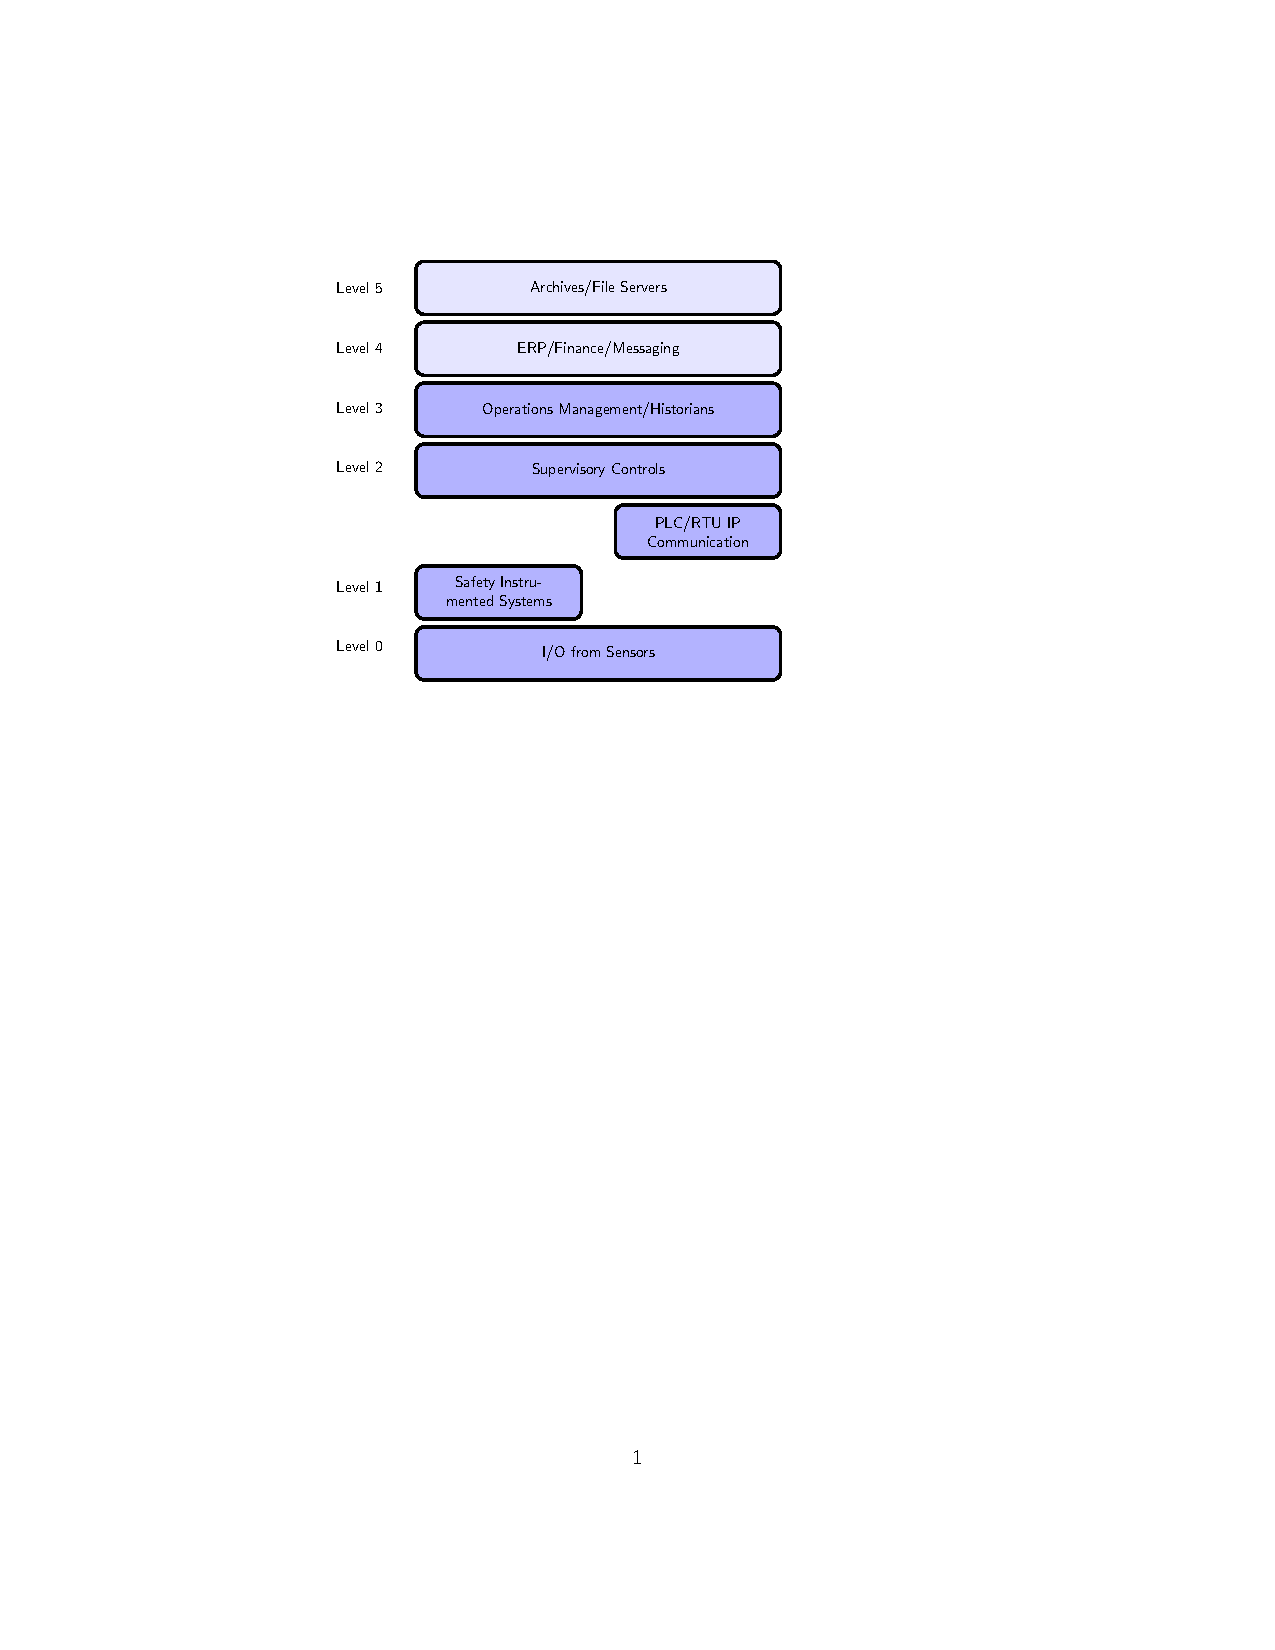
\includegraphics[angle=90,
%                 width=0.5\textwidth]{test}
%\caption{This is a test.}
%\end{figure}
%\end{verbatim}
%\end{code}
%It includes the graphic stored in the file \texttt{test.eps}. The
%graphic is \emph{first} rotated by an angle of 90 degrees and
%\emph{then} scaled to the final width of 0.5 times the width of a
%standard paragraph.  The aspect ratio is $1.0$, because no special
%height is specified.  The width and height parameters can also be
%specified in absolute dimensions. Refer to Table \ref{units} on
%page \pageref{units} for more information. If you want to know more
%about this topic, make sure to read \cite{graphics} and \cite{eps}.

下面的示例代码可以帮助我们理解整个过程:
\begin{code}
\begin{verbatim}
\begin{figure}
\centering
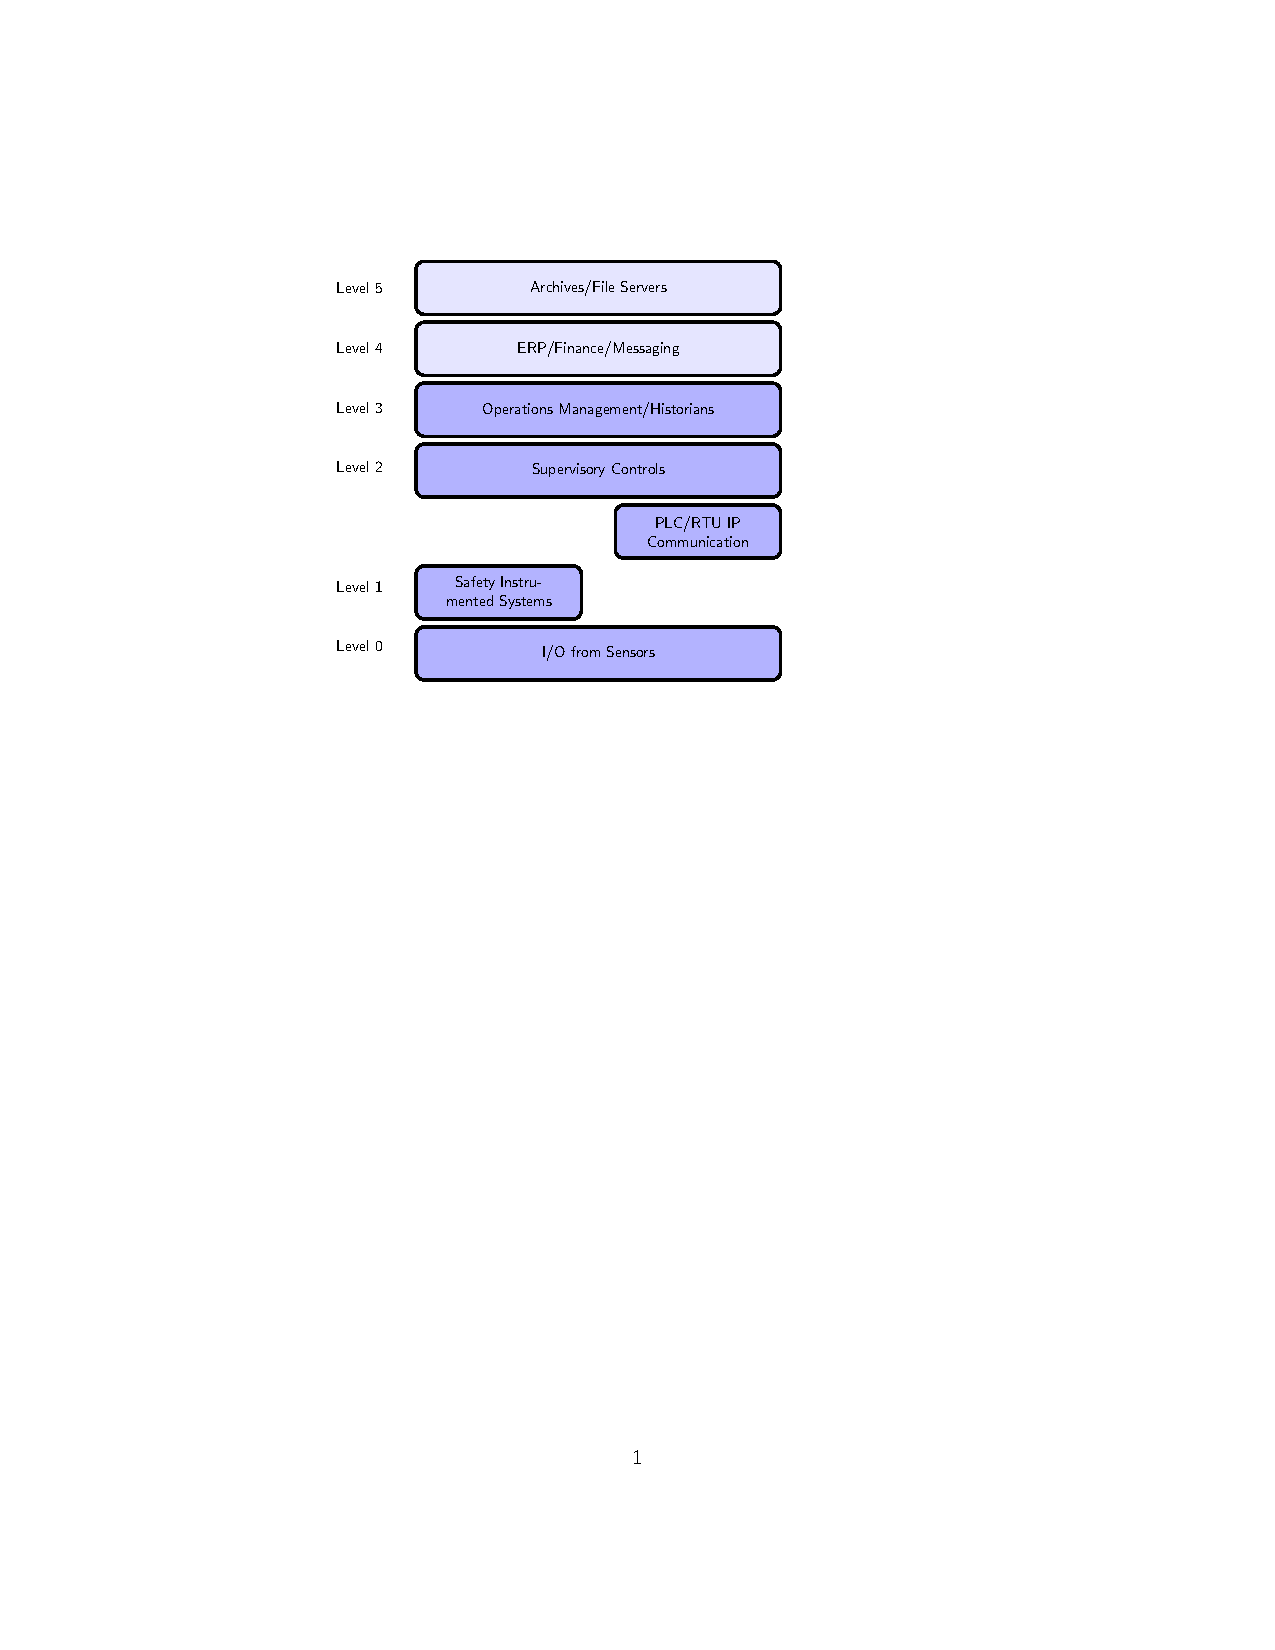
\includegraphics[angle=90,
                 width=0.5\textwidth]{test}
\caption{This is a test.}
\end{figure}
\end{verbatim}
\end{code}
这段代码把文件 \texttt{test.eps} 中的图形插入到文档里。{\textbf
首先}图形被旋转 90 度,{\textbf
然后}进行缩放使得图形的宽度等于标准段落宽度的 0.5 倍。
因为没有指定图形的高度,图形的高宽变化的比例是 $1.0$,也就是保持原来的高宽比。
高度和宽度参数也可以指定为绝对长度单位。详细的信息可以在第 \pageref{units} 页
的表 \ref{units} 中找到。如果你想知道更多这方面的知识,请阅读文献 \cite{graphics} 
和 \cite{eps}。

%\section{Bibliography}
\section{参考文献}

%You can produce a \wi{bibliography} with the \ei{thebibliography}
%environment.  Each entry starts with
%\begin{lscommand}
%\ci{bibitem}\verb|[|\emph{label}\verb|]{|\emph{marker}\verb|}|
%\end{lscommand}
%The \emph{marker} is then used to cite the book, article or paper
%within the document.
%\begin{lscommand}
%\ci{cite}\verb|{|\emph{marker}\verb|}|
%\end{lscommand}
%If you do not use the \emph{label} option, the entries will get
%enumerated automatically.  The parameter after the
%\verb|\begin{thebibliography}| command defines how much space to
%reserve for the number of labels. In the example below, \verb|{99}|
%tells \LaTeX{} to expect that none of the bibliography item numbers
%will be wider than the number 99. \enlargethispage{2cm}
%\begin{example}
%Partl \cite{pa} has
%proposed that \ldots
%\begin{thebibliography}{99}
%\bibitem{pa} H. Partl:
%\emph{German \TeX},
%TUGboat Volume 9, Issue 1 (1988)
%\end{thebibliography}
%\end{example}

你可以通过 \ei{thebibliography} 环境来产生一个参考文献 (\wi{bibliography})。每个参考文献的
条目以如下的命令开头
  \begin{lscommand}
    \ci{bibitem}\verb|[|\emph{label}\verb|]{|\emph{marker}\verb|}|
  \end{lscommand}
然后使用 \emph{marker} 在正文中引用这本书、这篇文章或者论文。
  \begin{lscommand}
    \ci{cite}\verb|{|\emph{marker}\verb|}|
  \end{lscommand}
如果你不使用参数 \emph{label},参考文献条目的编号是自动生成的。 \verb|\begin{thebibliography}| 
命令后的参数设定了最大的编号宽度。在下面的例子中, \verb|{99}| 告诉
 \LaTeX{} 参考文献条目的编号不会比数字 $99$ 更宽。
%\enlargethispage{2cm}
 \begin{example}
 Partl \cite{pa} has
 proposed that \ldots
 \begin{thebibliography}{99}
 \bibitem{pa} H. Partl:
 \emph{German \TeX},
 TUGboat Volume 9, Issue 1
  (1988)
 \end{thebibliography}
 \end{example}

%\chaptermark{Specialities} % w need to fix the damage done by the
                           %bibliography example.
\chaptermark{专业功能}
\thispagestyle{fancyplain}

%For larger projects, you might want to check out the Bib\TeX{}
%program. Bib\TeX{} is included with most \TeX{} distributions. It
%allows you to maintain a bibliographic database and then extract the
%references relevant to things you cited in your paper. The visual
%presentation of Bib\TeX{} generated bibliographies is based on a
%style sheets concept that allows you to create bibliographies
%following a wide range of established designs.

对于大型项目,你也许需要使用 Bib\TeX{} 程序。 Bib\TeX{} 包含在大多数
的 \TeX{} 发行版本中。它能够让你维护一个参考文献数据库,并从中生成你的
论文引用到的文献条目。 Bib\TeX{} 产生的参考文献的外观是基于样式表,
它可以让你按照大量预先设计好的格式来创建你的参考文献。

%\newpage

%\section{Indexing} \label{sec:indexing}

\section{索引}\label{sec:indexing}

%A very useful feature of many books is their \wi{index}. With
%\LaTeX{} and the support program \texttt{makeindex},\footnote{On
%systems not
%  necessarily supporting
%  filenames longer than 8 characters, the program may be called
%  \texttt{makeidx}.} an index can be generated quite easily.  This
%introduction will only explain the basic index generation commands.
%For a more in-depth view, please refer to \companion.
%\index{makeindex program} \index{makeidx package}

许多书籍的一个非常有用的部分就是它们的索引 (\wi{index}) 了。使用 \LaTeX{} 和辅助工具
 \texttt{makeindex}\footnote{在文件名不能超过 8 个字符的操作系统上,
这个程序被命名为 \texttt{makeidx}。},我们能够很容易的生成索引。在这个手册里,
只介绍了最基本的索引生成命令。更进一步的了解请参考 \companion。
\index{makeindex program} \index{makeidx package}

%To enable the indexing feature of \LaTeX{}, the \pai{makeidx} package
%must be loaded in the preamble with:
%\begin{lscommand}
%\verb|\usepackage{makeidx}|
%\end{lscommand}
%\noindent and the special indexing commands must be enabled by putting
%the
%\begin{lscommand}
%  \ci{makeindex}
%\end{lscommand}
%\noindent command into the input file preamble.

为了使用 \LaTeX{} 的索引功能,宏包 \pai{makeidx} 必须在导言部分被载入:
\begin{lscommand}
  \verb|\usepackage{makeidx}|
\end{lscommand}
\noindent 然后在导言中使用
\begin{lscommand}
  \ci{makeindex}
\end{lscommand}
\noindent 激活索引命令。

%The content of the index is specified with
%\begin{lscommand}
%  \ci{index}\verb|{|\emph{key}\verb|}|
%\end{lscommand}
%\noindent commands, where \emph{key} is the index entry. You enter the
%index commands at the points in the text that you want the final index
%entries to point to.  Table \ref{index} explains the syntax of the
%\emph{key} argument with several examples.

索引的内容通过命令
\begin{lscommand}
  \ci{index}\verb|{|\emph{key}\verb|}|
\end{lscommand}
\noindent
指定,这里 \emph{key} 是索引项的关键词。你可以在需要被索引的地方
加入这条命令。表 \ref{index} 举例解释了参量 \emph{key} 语法。

%\begin{table}[!tp]
%\caption{Index Key Syntax Examples.}
%\label{index}
%\begin{center}
%\begin{tabular}{@{}lll@{}}
%  \textbf{Example} &\textbf{Index Entry} &\textbf{Comment}\\\hline
%  \rule{0pt}{1.05em}\verb|\index{hello}| &hello, 1 &Plain entry\\
%\verb|\index{hello!Peter}|   &\hspace*{2ex}Peter, 3 &Subentry under `hello'\\
%\verb|\index{Sam@\textsl{Sam}}|     &\textsl{Sam}, 2& Formatted entry\\
%\verb|\index{Lin@\textbf{Lin}}|     &\textbf{Lin}, 7& Same as above\\
%\verb.\index{Jenny|textbf}.     &Jenny, \textbf{3}& Formatted page number\\
%\verb.\index{Joe|textit}.     &Joe, \textit{5}& Same as above\\
%\verb.\index{ecole@\'ecole}.     &\'ecole, 4& Handling of accents
%\end{tabular}
%\end{center}
%\end{table}

\begin{table}[!tp]
\caption{索引关键词语法示例。} \label{index}
\begin{center}
\begin{tabular}{@{}lll@{}}
  \textbf{示例} &\textbf{索引项} &\textbf{注释}\\\hline
  \rule{0pt}{1.05em}\verb|\index{hello}| &hello, 1 & 普通格式的索引项\\
\verb|\index{hello!Peter}|   &\hspace*{2ex}Peter, 3 & `hello' 下的子项\\
\verb|\index{Sam@\textsl{Sam}}|     &\textsl{Sam}, 2& 格式化的索引项\\
\verb|\index{Lin@\textbf{Lin}}|     &\textbf{Lin}, 7& 同上\\
\verb.\index{Jenny|textbf}.     &Jenny, \textbf{3}& 格式化的页码\\
\verb.\index{Joe|textit}.     &Joe, \textit{5}& 同上\\
\verb.\index{ecole@\'ecole}.     &\'ecole, 4& 重音标记
\end{tabular}
\end{center}
\end{table}

%When the input file is processed with \LaTeX{}, each \verb|\index|
%command writes an appropriate index entry, together with the current
%page number, to a special file. The file has the same name as the
%\LaTeX{} input file, but a different extension (\verb|.idx|). This
%\eei{.idx} file can then be processed with the \texttt{makeindex}
%program.

当 \LaTeX{} 处理源文档时,每个 \verb|\index| 命令都会将适当的索引项
和当前页码写入一个专门的文件中。这个文件的名字和 \LaTeX{} 源文档相同,
但具有不同的扩展名后缀 (\verb|.idx|)。这个 \texttt{.idx} 文件需要用
 \texttt{makeindex} 程序来处理。

%\begin{lscommand}
%  \texttt{makeindex} \emph{filename}
%\end{lscommand}
%The \texttt{makeindex} program generates a sorted index with the same base
%file name, but this time with the extension \eei{.ind}. If now the
%\LaTeX{} input file is processed again, this sorted index gets
%included into the document at the point where \LaTeX{} finds
%\begin{lscommand}
%  \ci{printindex}
%\end{lscommand}

\begin{lscommand}
  \texttt{makeindex} \emph{filename}
\end{lscommand}
\texttt{makeindex} 程序生成一个与源文件同名的序列化索引文件,
这个文件使用 \texttt{.ind} 为扩展名。当再次用 \LaTeX{} 处理源文件时,
这个序列化索引文件将被包含到源文件中
\begin{lscommand}
  \ci{printindex}
\end{lscommand}
\noindent 命令出现的位置。

%The \pai{showidx} package that comes with \LaTeXe{} prints out all
%index entries in the left margin of the text. This is quite useful for
%proofreading a document and verifying the index.

\LaTeXe{} 附带的宏包 \pai{showidx} 可以在正文的左边打印出索引项。
这个功能在校对文档和索引项时十分有用。

% Note that the \ci{index}
%command can affect your layout if not used carefully.

%\begin{example}
%My Word \index{Word}. As opposed
%to Word\index{Word}. Note the
%position of the full stop.
%\end{example}

请注意不谨慎地使用 \ci{index} 命令,将会影响文档页版面布局。
\begin{example}
My Word \index{Word}. As opposed
to Word\index{Word}. Note the
position of the full stop.
\end{example}

%\section{Fancy Headers}
%\label{sec:fancy}
\section{定制页眉和页脚}
\label{sec:fancy}

%The \pai{fancyhdr} package,\footnote{Available from
%  \CTANref|macros/latex/contrib/supported/fancyhdr|.} written by
%Piet van Oostrum, provides a few simple commands that allow you to
%customize the header and footer lines of your document.  If you look
%at the top of this page, you can see a possible application of this
%package.

Piet van
Oostrum 编写的 \pai{fancyhdr} 宏包\footnote{可以在 \CTANref|macros/latex/contrib/supported/fancyhdr| 得到。},
提供了一些简单的命令使得我们可以定制文档的页眉和页脚。看一眼本页的顶部,
你就能发现这个宏包的用处。

%\begin{figure}[!htbp]
%\begin{lined}{\textwidth}
%\begin{verbatim}
%\documentclass{book}
%\usepackage{fancyhdr}
%\pagestyle{fancy}
% with this we ensure that the chapter and section
% headings are in lowercase.
%\renewcommand{\chaptermark}[1]{%
%        \markboth{#1}{}}
%\renewcommand{\sectionmark}[1]{%
%        \markright{\thesection\ #1}}
%\fancyhf{}  % delete current header and footer
%\fancyhead[LE,RO]{\bfseries\thepage}
%\fancyhead[LO]{\bfseries\rightmark}
%\fancyhead[RE]{\bfseries\leftmark}
%\renewcommand{\headrulewidth}{0.5pt}
%\renewcommand{\footrulewidth}{0pt}
%\addtolength{\headheight}{0.5pt} % space for the rule
%\fancypagestyle{plain}{%
%   \fancyhead{} % get rid of headers on plain pages
%   \renewcommand{\headrulewidth}{0pt} % and the line
%}
%\end{verbatim}
%\end{lined}
%\caption{Example \pai{fancyhdr} Setup.} \label{fancyhdr}
%\end{figure}

\begin{figure}[!htbp]
\begin{lined}{\textwidth}
\begin{verbatim}
\documentclass{book}
\usepackage{fancyhdr}
\pagestyle{fancy}
 with this we ensure that the chapter and section
 headings are in lowercase.
\renewcommand{\chaptermark}[1]{%
        \markboth{#1}{}}
\renewcommand{\sectionmark}[1]{%
        \markright{\thesection\ #1}}
\fancyhf{}  % delete current header and footer
\fancyhead[LE,RO]{\bfseries\thepage}
\fancyhead[LO]{\bfseries\rightmark}
\fancyhead[RE]{\bfseries\leftmark}
\renewcommand{\headrulewidth}{0.5pt}
\renewcommand{\footrulewidth}{0pt}
\addtolength{\headheight}{0.5pt} % space for the rule
\fancypagestyle{plain}{%
   \fancyhead{} % get rid of headers on plain pages
   \renewcommand{\headrulewidth}{0pt} % and the line
}
\end{verbatim}
\end{lined}
\caption{\pai{fancyhdr} 设置实例。} \label{fancyhdr}
\end{figure}

%The tricky problem when customising headers and footers is to get
%things like running section and chapter names in there. \LaTeX{}
%accomplishes this with a two-stage approach. In the header and footer
%definition, you use the commands \ci{rightmark} and \ci{leftmark} to
%represent the current section and chapter heading, respectively.
%The values of these two commands are overwritten whenever a chapter or
%section command is processed.

定制页眉和页脚时一件棘手的事情就是得到每个页面所属的章节名称。
\LaTeX{} 通过两个步骤来完成这个任务。在定义页眉和页脚时,你可以使用
 \ci{rightmark} 命令来代表当前的 section 名,使用 \ci{leftmark} 来代表当前的 chapter 名。
这两个命令的值将在处理 chapter 或者 section 命令时被重新赋值。

%For ultimate flexibility, the \verb|\chapter| command and its friends
%do not redefine \ci{rightmark} and \ci{leftmark} themselves. They call
%yet another command (\ci{chaptermark}, \ci{sectionmark}, or
%\ci{subsectionmark}) that is responsible for redefining \ci{rightmark}
%and \ci{leftmark}.

为了获得最大的灵活性, \verb|\chapter| 等命令并不对 \ci{rightmark} 和
 \ci{leftmark} 直接进行重定义,而是间接地通过调用 \ci{chaptermark}、
\ci{sectionmark} 或者 \ci{subsectionmark} 来重新定义 \ci{rightmark} 和
 \ci{leftmark}。

%If you want to change the look of the chapter
%name in the header line, you need only ``renew'' the \ci{chaptermark}
%command. \cih{sectionmark}\cih{subsectionmark}

因此,只需要重新定义 \ci{chaptermark} 命令,\cih{sectionmark}\cih{subsectionmark}
就能修改页眉上显示的章名。

%Figure \ref{fancyhdr} shows a possible setup for the \pai{fancyhdr}
%package that makes the headers look about the same as they look in
%this booklet. In any case, I suggest you fetch the documentation for
%the package at the address mentioned in the footnote.

图 \ref{fancyhdr} 显示了如何配置 \pai{fancyhdr} 来得到和本文相似的页眉。
无论如何我还是建议你先阅读一下 \pai{fancyhdr} 宏包所带的文档。

%\section{The Verbatim Package}
\section{Verbatim 宏包}

%Earlier in this book, you got to know the \ei{verbatim}
%\emph{environment}.  In this section, you are going to learn about the
%\pai{verbatim} \emph{package}. The \pai{verbatim} package is basically
%a re-implementation of the \ei{verbatim} environment that works around
%some of the limitations of the original \ei{verbatim} environment.
%This by itself is not spectacular, but the implementation of the
%\pai{verbatim} package added new functionality, which is
%why I am mentioning the package here. The \pai{verbatim}
%package provides the

在本文的前面部分你已经知道了 \ei{verbatim} {\textbf
环境}。在这一节中, 你将学会使用 \pai{verbatim} {\textbf
宏包}。 \pai{verbatim} 宏包重新
实现了 \ei{verbatim} 环境,并解决了原来的 \ei{verbatim} 环境的一些限制。
这本身并没有什么特别的,但 \pai{verbatim} 宏包还实现了一些新增的功能,
这才是我在这里提到这个宏包的原因。 \pai{verbatim} 宏包提供了

\begin{lscommand}
\ci{verbatiminput}\verb|{|\emph{filename}\verb|}|
\end{lscommand}

%\noindent command, which allows you to include raw ASCII text into your
%document as if it were inside a \ei{verbatim} environment.

\noindent
命令,这个命令允许你把一个 ASCII 码的文本文件包含到你的文档中来,
就好像它们是在 \ei{verbatim} 环境中一样。

%As the \pai{verbatim} package is part of the `tools' bundle, you
%should find it pre-installed on most systems. If you want to know more
%about this package, make sure to read \cite{verbatim}.

\pai{verbatim} 宏包是 `tools' 宏包集的一部分,大多数的系统中都预装了这个宏包集。
如果你想更多地了解这个宏包,可以阅读 \cite{verbatim}。

%\section{Installing Extra Packages}\label{sec:Packages}
\section{安装额外的宏包}\label{sec:Packages}

%Most \LaTeX{} installations come with a large set of pre-installed
%style packages, but many more are available on the net. The main
%place to look for style packages on the Internet is CTAN
%(\url{http://www.ctan.org/}).

大多数的 \LaTeX{} 安装都带有大量预装的样式宏包,但更多的宏包可以在网上得到。
在互联网寻找样式宏包的一个主要的地方就是 CTAN
(\url{http://www.ctan.org/})。

%Packages such as \pai{geometry}, \pai{hyphenat}, and many
%others are typically made up of two files: a file with the extension
%\texttt{.ins} and another with the extension \texttt{.dtx}. There
%will often be a \texttt{readme.txt} with a brief description of the
%package. You should of course read this file first.

各种宏包的源文件,例如 \pai{geometry}, \pai{hyphenat} 等等,一般来说都包含
两个文件:一个扩展名为 \texttt{.ins},另一个扩展名为 \texttt{.dtx}。
此外,通常会有一个 \texttt{readme.txt} 对宏包进行简要的说明。你应该先阅读这个文件。

%In any event, once you have copied the package files onto your
%machine, you still have to process them in a way that (a) tells your
%\TeX\ distribution about the new style package and (b) gives you
%the documentation.  Here's how you do the first part:

无论如何,一旦你得到了宏包的源文件,你还要对它们进行处理使得 (a) 你的 \TeX{} 系统知道这个新的宏包, (b) 生成说明文档。下面是第一部分的步骤:

%\begin{enumerate}
%\item Run \LaTeX{} on the \texttt{.ins} file. This will
%  extract a \eei{.sty} file.
%\item Move the \eei{.sty} file to a place where your distribution
%  can find it. Usually this is in your \texttt{\ldots/\emph{localtexmf}/tex/latex}
%  subdirectory (Windows or OS/2 users should feel free to change the
%  direction of the slashes).
%\item Refresh your distribution's file-name database. The command
%  depends on the \LaTeX distribution you use:
%  teTeX, fpTeX -- \texttt{texhash}; web2c -- \texttt{maktexlsr};
%  MikTeX -- \texttt{initexmf -update-fndb} or use the GUI.
%\end{enumerate}

\begin{enumerate}
\item 对 \texttt{.ins} 文件运行 \LaTeX{} 命令。这将会产生一个 \texttt{.sty} 文件。
\item 把 \texttt{.sty} 文件移到 \LaTeX{} 系统能找到的地方。一般是在 
      \texttt{\ldots/\emph{localtexmf}/tex/latex} 子目录下(Windows 或者 OS/2 用户应该改变斜线为反斜线)。
\item 刷新系统的文件名数据库。具体的命令取决于你使用的 \LaTeX{} 系统:
       teTeX, fpTeX -- \texttt{texhash}; web2c -- \texttt{maktexlsr};
      MikTeX -- \texttt{initexmf -update-fndb} 或者使用图形界面。
\end{enumerate}

%\noindent Now you can extract the documentation from the
%\texttt{.dtx} file:

\noindent 现在你可以从 \texttt{.dtx} 文件生成说明文档:

%\begin{enumerate}
%\item Run \LaTeX\ on the \texttt{.dtx} file.  This will generate a
%  \texttt{.dvi} file. Note that you may have to run \LaTeX\
%  several times before it gets the cross-references right.
%\item Check to see if \LaTeX\ has produced a \texttt{.idx} file
%  among the various files you now have.
%  If you do not see this file, then you may proceed to
%  step \ref{step:final}.
%\item In order to generate the index, type the following:\\
%        \fbox{\texttt{makeindex -s gind.ist \textit{name}}}\\
%        (where \textit{name} stands for the main-file name without any
%    extension).
% \item Run \LaTeX\ on the \texttt{.dtx} file once again. \label{step:next}
%
%\item Last but not least, make a \texttt{.ps} or \texttt{.pdf}
%  file to increase your reading pleasure.\label{step:final}
%
%\end{enumerate}

\begin{enumerate}
\item 对 \texttt{.dtx} 文件运行 \LaTeX{} 命令。这会生成一个 \texttt{.dvi} 文件。
      注意你可能需要多次运行 \LaTeX{} 命令来正确处理交叉引用。
\item 检查一下 \LaTeX{} 命令是否产生了 \texttt{.idx} 文件。如果没发现这个文件,
      你就可以执行第 \ref{step:final} 步了。
\item 为了生成索引,敲入命令:\\
      \fbox{\texttt{makeindex -s gind.ist \textit{name}}}\\
      (这里 \textit{name} 表示不带扩展名的主文件名)。
\item 再次对 \texttt{.dtx} 文件运行 \LaTeX{} 命令。\label{step:next}
\item 最后一步但不是必需的,生成 \texttt{.ps} 文件或者 \texttt{.pdf} 文件以方便阅读。\label{step:final}

\end{enumerate}

%Sometimes you will see that a \texttt{.glo}
%(glossary) file has been produced. Run the following
%command between
%step \ref{step:next} and \ref{step:final}:

有时你会看见生成了一个 \texttt{.glo}
(glossary) 文件。在第 \ref{step:next} 步和第 \ref{step:final} 步之间
运行下面的命令:

\noindent\texttt{makeindex -s gglo.ist -o \textit{name}.gls \textit{name}.glo}

%\noindent Be sure to run \LaTeX\ on the \texttt{.dtx} one last
%time before moving on to step \ref{step:final}.

\noindent
确认在执行第 \ref{step:final} 步前最后对 \texttt{.dtx} 文件运行一遍 \LaTeX{} 命令。

%%%%%%%%%%%%%%%%%%%%%%%%%%%%%%%%%%%%%%%%%%%%%%%%%%%%%%%%%%%%%%%%%
% Contents: Chapter on pdfLaTeX
% French original by Daniel Flipo 14/07/2004
%%%%%%%%%%%%%%%%%%%%%%%%%%%%%%%%%%%%%%%%%%%%%%%%%%%%%%%%%%%%%%%%%

%\section{Working with pdf\LaTeX}

\section{使用 pdf\LaTeX} \label{sec:pdftex}\index{PDF}
\secby{Daniel Flipo}{Daniel.Flipo@univ-lille1.fr}
%\footnote{翻译: Li Jian. lijian605@yahoo.com.cn}}
%
%\begin{tiny}
%by Daniel Flipo $<$Daniel.Flipo@univ-lille1.fr$>$
%\end{tiny}%


%PDF is a \wi{hypertext} document format. Much like in a web page,
%some words in the document are marked as hyperlinks. They link to
%other places in the document or even to other documents. If you
%click on such a hyperlink you get transported to the destination of
%the link. In the context of \LaTeX{}, this means that all
%occurrences of \ci{ref} and \ci{pageref} become hyperlinks.
%Additionally, the table of contents, the index and all the other
%similar structures become collections of hyperlinks.

PDF 是一种超文本文档 (\wi{hypertext}) 格式。类似于网页,
文档中的某些词可以被超链接标记。它们链接到这个文档的另一个地方,
甚至是另外一个文档。如果你点击这样一个超链接,
你将转调到链接的目的地。
这意味着在 \LaTeX{} 格式的文档中所有 \ci{ref} 和 \ci{pageref} 出现的位置都变成超链接。此外,目录、
索引和其它类似的结构变成超链接的集合。

%Most web pages you find today are written in HTML \emph{(HyperText
%  Markup Language)}. This format has two significant disadvantages
%when writing scientific documents:
%\begin{enumerate}
%\item Including mathematical formulae into HTML documents is not
%  generally supported. While there is a standard for it, most browsers
%  used today do not support it, or lack the required fonts.
%\item Printing HTML documents is possible, but the results vary widely
%  between platforms and browsers. The results are miles removed from
%  the quality we have come to expect in the \LaTeX{} world.
%\end{enumerate}

现在大多数的网页都是用 HTML \textbf{超文本标记语言}编写。
在写科技文档的时候,这种格式有两个严重的缺陷:
\begin{enumerate}
\item 数学公式在 HTML 文档中通常都不被支持。尽管对此有一个标准,
但是大多是现在使用的浏览器都不支持,或者缺少需要的字体。
\item 打印 HTML 文档是比较容易的,但打印的结果会因系统平台和浏览器的不同
而出现差异。
这结果与我们在 \LaTeX{} 世界中期待的高质量相差十万八千里。
\end{enumerate}

% There have been many attempts to create translators
%from \LaTeX{} to HTML. Some were even quite successful in the sense
%that they are able to produce legible web pages from a standard
%\LaTeX{} input file. But all of them cut corners left and right to
%get the job done. As soon as you start using more complex \LaTeX{}
%features and external packages things tend to fall apart. Authors
%wishing to preserve the unique typographic quality of their
%documents even when publishing on the web turn to PDF
%\emph{(Portable Document Format)}, which preserves the layout of the
%document and permits hypertext navigation. Most modern browsers come
%with plugins that allow the direct display of PDF documents.

有许多将 \LaTeX{} 转为 HTML 的尝试。其中一些可以说是相当成功的,
它们能将一个标准的 \LaTeX{} 源文件生成一个合格的网页。
但是为了达到目的,需要去掉一些支持。
当你开始使用 \LaTeX{} 的复杂功能和扩展宏包时,那些尝试就行不通了。
若希望即使是发不到网上也保留文档的高质量,
作者们就要使用 PDF \textbf{(便携式文档格式)},
它保留了文档的版式和允许超链接导航。
现在大多数浏览器只要带上相应的插件都可以直接显示 PDF 文档。

%Even though there are DVI and PS viewers for almost every platform, you will find that
%\wi{Acrobat Reader} and \wi{Xpdf} for viewing PDF documents
%are more widely deployed. So providing PDF versions of your documents will
%make them much more accessible to your potential readers.

尽管几乎所有的操作系统都有 DVI 和 PS 格式的阅读器,
但你会发现人们更多地使用 \wi{Acrobat
Reader} 和 \wi{Xpdf} 来阅读 PDF 文档。
因而提供 PDF 格式的文档将使得潜在的读者更容易阅读。


%\subsection{PDF Documents for the Web}
\subsection{发布到网上的 PDF 文档}

% The creation of a PDF file from \LaTeX{} source is very simple,
%thanks to the pdf\TeX{} program developed by
%H\`an Th\'{\^e} Th\`anh. pdf\TeX{} produces PDF output where normal
%\TeX{} produces DVI. There is also a pdf\LaTeX{}, which produces
%  PDF output from \LaTeX{} sources. \index{pdftex@pdf\TeX}\index{pdftex@pdf\LaTeX}

有了 H\`an Th\'{\^e} Th\`anh 开发的 pdf\TeX{} 程序,使用 \LaTeX 源文件来创建 PDF 文件将变得非常简单。
一般的 TeX{} 生成 DVI,
而 pdf\TeX{} 生成 PDF。还有 pdf\LaTeX{} 程序将 LaTeX{} 源文件生成 PDF。
\index{pdftex@pdf\TeX}\index{pdftex@pdf\LaTeX}

%Both pdf\TeX{} and pdf\LaTeX{} are installed automatically by most
%modern \TeX{} distributions, such as te\TeX{}, fp\TeX{}, Mik\TeX,
%\TeX{}Live and CMac\TeX{}.

现在大多数的 \TeX{} 发行版本都自动集成安装了 pdf\TeX{} 和 pdf\LaTeX{},
例如: te\TeX{}, fp\TeX{}, Mik\TeX{}, \TeX{}Live 和 CMac\TeX{}。

%To produce a PDF instead of DVI, it is sufficient to replace the
%command \texttt{latex file.tex} by
%\texttt{pdflatex file.tex}. On systems where \LaTeX{} is not called from the
%command line, you may find a special button in the \TeX{}ControlCenter.

为了生成 PDF 而不是 DVI,只需要将命令 \texttt{latex
file.tex} 改成 \texttt{pdflatex
file.tex}。在不是使用命令行的 \LaTeX{} 系统中,你可以在 \TeX{} 控制中心找到一个专门的按钮。

%In \LaTeX{} you can define the paper size with an
%optional documentclass argument such as \texttt{a4paper} or
%\texttt{letterpaper}. This works in pdf\LaTeX{} too, but on top of this
%pdf\TeX{} also needs to know the physical size of the paper to determine the physical
%size of the pages in the pdf file.
%\index{paper size}
%If you use the
%\pai{hyperref} package (see page \pageref{ssec:pdfhyperref}), the
%papersize will be adjusted automatically. Otherwise you have to do this
%manually by putting the following lines into the preamble of the document:
%\begin{code}
%\begin{verbatim}
%\pdfpagewidth=\paperwidth
%\pdfpageheight=\paperheight
%\end{verbatim}
%\end{code}

在 \LaTeX{} 中,
你可以通过 documentclass 的参数选项来定义页面的大小,
例如:\texttt{a4paper} 或 \texttt{letterpaper}。这些也
对 pdf\LaTeX{} 有效,但是首先要让 pdf\TeX{} 知道这种页
面的实际大小来控制 PDF 文件的页面大小。若你使用 \pai{hyperref} 宏
包(参见第 \pageref{ssec:pdfhyperref} 页),页面的大小将自动调整。
否则,你需要手动的将下面两行加入到文档的导言区:
\begin{code}
\begin{verbatim}
\pdfpagewidth=\paperwidth
\pdfpageheight=\paperheight
\end{verbatim}
\end{code}

%The following section will go into more detail regarding the
%differences between normal \LaTeX{} and pdf\LaTeX{}. The main
%differences concern three areas: the fonts to use, the format of
%images to include, and the manual configuration of hyperlinks.

接下来的一节将深入介绍 \LaTeX{} 和 pdf\LaTeX{} 之间的不同。主要的不同
有三个方面:采用的字体,包含图像的格式和超链接的手动配置。

%\subsection{The Fonts}
\subsection{字体}

%\wi{pdf\LaTeX} can deal with all sorts of fonts (PK bitmaps,
%TrueType,
%%\PSi{} type 1\dots) but the normal \LaTeX{} font format, the bitmap PK
%PostScript type 1\dots) but the normal \LaTeX{} font format, the
%bitmap PK fonts produce very ugly results when the document is
%%displayed with Acrobat Reader. It is best to use \PSi{} Type 1 fonts
%displayed with Acrobat Reader. It is best to use PostScript Type 1
%fonts exclusively to produce documents that display well.
%\emph{Modern TeX installations will be setup so that this happens
%automatically. Best is to try. If it works for you, just skip this
%whole section.}

\wi{pdf\LaTeX} 能处理所有的字体 (PK 点阵、TrueType、 \PSi{}
type 1……),但是作为 \LaTeX{} 通常的字体格式, PK 点阵字体在 Acrobat
Reader 下的显示效果非常差。为了获得文档更高的显示效果,最好使用 \PSi{}
Type 1 字体。{\textbf
高级的 \TeX{} 安装程序会自动设置好,你最好试一下,如果它正常运作,你就可以跳过这一节。}

%The \PSi{} Type 1 implementation of the Computer Modern and AMSFonts
%was produced by Blue Sky Research and Y\&Y, Inc., who then
%transferred copyright to the American Mathematical Society. The
%fonts were made publicly available in early 1997 and currently come
%with most of \TeX{} distributions.

\PSi{} Type 1 的 Computer Modern 和 AMSFonts 字体由 Blue Sky
Research 和 Y\&Y,
Inc. 制作,后来版权属于美国数学学会 (AMS)。这些字体在 1997 年被开放,并且出现在大多数 \TeX{} 发行版中。

%However, if you are using \LaTeX{} to create documents in languages
%other than English, you might want to use EC, LH, or CB fonts (see the
%discussion about \texttt{OT1} fonts on the page \pageref{OT1}).
%Vladimir Volovich has created the cm-super font bundle which covers the
%entire EC/TC, EC Concrete, EC Bright and LH font sets. It is available from
%\texttt{CTAN:/fonts/ps-type1/cm-super} and is included with \TeX{}Live7
%and Mik\TeX. Similar type 1 CB Greek fonts created by Apostolos
%Syropoulos are available at
%\texttt{CTAN:/tex-archive/fonts/greek/cb}. Unfortunately, both of
%these font sets are not of the same typographic quality as the Type1
%CM fonts by Blue Sky/Y\&Y. They were automatically hinted, and the
%document might look not as neat on the screen as the ones using Blue
%Sky/Y\&Y type 1 CM fonts, on high resolution output devices they
%produce results identical to the original bitmap EC/LH/CB fonts.

然而,如果你使用 \LaTeX{} 来创建非英文的文档,你可能用到 EC, LH 或 CB 字体(关于
 \texttt{OT1} 字体的讨论可参见第 \pageref{OT1} 页)。Vladimir
Volovich 创建了 cm-super 字体包,包含全部 EC/TC、EC Concrete、EC
Bright 和 LH 字体集。在 \texttt{CTAN:/fonts/ps-type1/cm-super} 可以获得,也被集成进了
 \TeX{}Live7 和 Mik\TeX\/。由 Apostolos Syropoulos 创建类似 type 1
CB 的希腊字体可在 \texttt{CTAN:/tex-archive/fonts/greek/cb} 获得。不幸的是,这些字体集跟 Blue
Sky/Y\&Y 的 Type 1
CM 字体的印刷质量不一样。\LaTeX{} 会自动提示,而且文档在屏幕的显示效果也不如 Blue
Sky/Y\&Y type 1
CM 字体那么整洁。在高分辨率的输出设备下,它们生成的效果跟原来的 EC/LH/CB 点阵字体一样。

% If you are creating document in one of Latin-based
%languages, you have several other options.
%\begin{itemize}
%\item You might want to use \pai{aeguill} package, aka
%  \emph{Almost European Computer Modern with Guillemets}. Just put the
%  line
%  \newline
 % \verb+\usepackage{aeguill}+\ into the preamble of
 % your document, to enable AE virtual fonts instead of EC fonts.
%\item Alternatively, you can use \pai{mltex} package, but this only works when
%  your pdf\TeX{} has been compiled with the \wi{mltex} option.
%\end{itemize}

如果你使用一种拉丁语系的语文来创建文档,你有其它一些选择。
\begin{itemize}
\item 使用 \pai{aeguill} 宏包,也叫 \emph{Almost European Computer Modern with
Guillemets}。只需在导言区添加一行 \verb+\usepackage{aeguill}+,来启用 AE 虚拟字体替代 EC 字体。
\item 或者使用 \pai{mltex} 宏包,但是它只在 pdf\TeX{} 设置了 \wi{mltex} 选项时有效。
\end{itemize}

%The AE virtual fontset, like the {Ml\TeX} system, makes \TeX{} believe
%it has a full 256 character fontset at its disposal by creating most of
%the missing letters from characters of the CM font and rearranging them
%in the EC order, this allows to use the excellent type 1 format CM
%fonts available on most systems. As the font is now in T1 encoding,
%hyphenation will work well in Latin-based European languages.  The only
%disadvantage of this approach is that the artificial AE characters do
%not work with Acrobat Reader's \texttt{Find} function, so you cannot
%search for words with accented characters in your final PDF file.

AE 虚拟字体集,像 {Ml\TeX} 系统,在 CM 字体的字符基础上创建
全部缺失的字母并按 EC 顺序重新排列,就使得 \TeX{} 处理它的时候
认为它有一个全部 256 个字符的字体集。这样就可使用大部分系统中优质的 type
1 格式的 cm 字体。这套字体现在为 T1 编码,在拉丁语系的欧洲语文中能很好的运作。
唯一的不足就是创建的 AE 字符不支持 Acrobat
Reader 的查找功能,因此你不能在 PDF 文档中搜索那些带重音符号的单词。

%For the Russian language a similar solution is to use C1 virtual fonts
%available at \texttt{ftp://ftp.vsu.ru/pub/tex/font-packs/c1fonts}.
%These fonts combine the standard CM type 1
%fonts from Bluesky collection and CMCYR type 1 fonts from  Paradissa and
%BaKoMa collection, all available on CTAN. Because Paradissa fonts
%contain only Russian letters, C1 fonts are
%missing other Cyrillic glyphs.

对于俄文,一个类似的解决办法是使用 C1 虚拟字体,这可以在 \texttt{ftp://ftp.vsu.ru/pub/tex/font-packs/c1fonts} 
上获得。这套字体集成了标准的 Bluesky CM type 1 字体和 Paradissa 
与 BaKoMa 的 CMCYR
type 1 字体,这些都可以在 CTAN 上找到。由于 Paradissa 字体只包含俄文字母,C1 字体里就没有
其他西里尔字符了。

%Another solution is to switch to other \PSi{} type 1 fonts.
%Actually, some of them are even included with every copy of Acrobat
%Reader. Because these fonts have different character sizes, the text
%layout on your pages will change. Generally these other fonts will
%use more space than the CM fonts, which are very space-efficient.
%Also, the overall visual coherence of your document will suffer
%because Times, Helvetica and Courier (the primary candidates for
%such a replacement job) have not been designed to work in harmony in
%a single document.

另一种解决办法是使用其它 \PSi{}
type 1 字体。事实上,其中一些字体被包含在 Acrobat
Reader 的相应语言版本中。由于这些字体有不同的字符大小,页面上的文本格式将会
改变。一般地,这类字体占得空间要比 CM 字体大,因为 CM 字体是一种
非常节省空间的字体。而且文档可视的一致性也被破坏了,因为 Times、
Helvetica 和 Courier 字体(这些是 Acrobat 里基本的可替换字体)没有
被设计来在单个文档中和平共处。

%Two ready-made font sets are available for this purpose:
%\pai{pxfonts}, which is based on \emph{Palatino} as its main text body font,
%and the \pai{txfonts} package, which is based on \emph{Times}. To use them it is
%sufficient to put the following lines into the preamble of your
%document:
%\begin{code}
%\begin{verbatim}
%\usepackage[T1]{fontenc}
%\usepackage{pxfonts}
%\end{verbatim}
%\end{code}

为了达到上述目的,有两套字体已经做好:\pai{pxfonts},它基于作为正文
字体的 \emph{Palatino};另外就是基于 \emph{Times} 的 \pai{txfonts} 宏包。只需要在文档的导言区加入下列几行就可以使用这些字体:
\begin{code}
\begin{verbatim}
\usepackage[T1]{fontenc}
\usepackage{pxfonts}
\end{verbatim}
\end{code}

%Note: you may find lines like
%\begin{verbatim}
%Warning: pdftex (file eurmo10): Font eur... not found
%\end{verbatim}
%in the  \texttt{.log} file after compiling your input file. They mean
%that some font used in the document has not been found. You really have
%to fix these problems, as the resulting PDF document may
%\emph{not display the pages with the missing characters at all}.

注:当你编译的时候,在 .log 文件中出现下面的信息:
\begin{verbatim}
Warning: pdftex (file eurmo10): Font eur... not found
\end{verbatim}
这意味着文档使用的某些字体没有被找到。你必须解决这些问题,否则输出的 PDF 
文件可能\textbf{不会显示缺失字符的页面}。

%As you can see this whole font business, especially the lack of a
%good EC fontset equivalent in quality to the CM font in type 1
%format, has been occupying many peoples minds. Recently a new set of
%high quality outline fonts called Latin Modern (LM) has become
%available. It puts an end to the misery. If you have a recent \TeX{}
%installation, chances are that you already have a copy of them
%installed all you need todo is to add
%\begin{code}
%\begin{verbatim}
%\usepackage{lmodern}
%\usepackage[T1]{fontenc}
%\usepackage{textcomp}
%\end{verbatim}
%\end{code}
%to the preamble of your document and you are all set for creating excellent
%pdf output with full support for the full Latin character set.

上面讨论了如此多的字体问题,特别是缺乏与 type 1 格式的 CM 字体同样高质量的 EC 字体一
直困扰大家。最近一套新的被称为  Latin Modern
(LM) 的高质量字体已开发完成。这使得前面的担心都是多余的。如果你安装了最新的 \TeX{},
你可能已经安装好这套字体,需要做的只是在你的文档的导言区添加
\begin{code}
\begin{verbatim}
\usepackage{lmodern}
\usepackage[T1]{fontenc}
\usepackage{textcomp}
\end{verbatim}
\end{code}
就可以创建支持所有拉丁字符的优质 PDF 输出文件。


%\subsection{Using Graphics}
\subsection{使用图形}
\label{ssec:pdfgraph}

%Including graphics into a document works best with the
%\pai{graphicx} package (see page \pageref{eps}).
%By using the special \emph{driver} option \texttt{pdftex} the
%package will work with pdf\LaTeX{} as well:
%\begin{code}
%\begin{verbatim}
%\usepackage[pdftex]{color,graphicx}
%\end{verbatim}
%\end{code}
%In the sample above I have included the color option, as using color in
%documents displayed on the web comes quite naturally.

通过 \pai{graphicx} 宏包
(参见第 \pageref{eps} 页),你可以在文档中插入图形。使用 \texttt{pdftex} 
作为 \emph{driver} 的选项,这个宏包也可用于 pdf\LaTeX{}:
\begin{code}
\begin{verbatim}
\usepackage[pdftex]{color,graphicx}
\end{verbatim}
\end{code}
上面这个例子中,我还包含了 color 宏包,因此网页上彩色的文档会看起来更自然一些。

%%So much for the good news. The bad news is that graphics in \EPSi{}
%format do not work with Pdf\LaTeX{}. If you don't define a file
%extension in the \ci{includegraphics} command, \pai{graphicx} will
%go looking for a suitable file on its own, depending on the setting
%of the \emph{driver} option. For \texttt{pdftex} this is formats
%\texttt{.png}, \texttt{.pdf}, \texttt{.jpg} and \texttt{.mps}
%%(\MP\index{metapost@\MP})---but \emph{not} \texttt{.eps}.

好消息到此为止。坏消息就是 \EPSi{} 格式的图形并不被 Pdf\LaTeX{} 所支持。
如果你不在命令 \ci{includegraphics} 声明加载的文件的扩展名,
宏包 \pai{graphicx} 将依赖于 \emph{driver} 选项
的设置自动寻找一个合适的文件。
对于 \texttt{pdftex} ,它支持的格式有 \texttt{.png},\texttt{.pdf},
\texttt{.jpg} 和 \texttt{.mps} (\texttt{MetaPost}\index{metapost@\MP}),但{\textbf
不}支持 \texttt{.eps}。

% The simple way out of this problem is
%to just convert your EPS files into PDF format using the
%\texttt{epstopdf} utility found on many systems. For vector graphics
%(drawings) this is a great solution. For bitmaps (photos, scans)
%this is not ideal, because the PDF format natively supports the
%inclusion of PNG and JPEG images. PNG is good for screenshots and
%other images with few colors. JPEG is great for photos, as it is
%very space-efficient.

一个解决这个问题的简单方法是通过在很多系统中可找到的 \texttt{epstopdf} 工具
将你的 EPS 文件转化为 PDF 格式。
对于矢量图(画),这时一个很好的解决办法,但对于位图(相片、扫描图),
这并不是很理想,因为 PDF 格式本来就支持包含 PNG 和 JPEG 图像。PNG 格式适合屏幕截图和其它一些只有较少颜色的图像。JPEG 是一种
非常适合于相片的格式,而且占用空间少。

% It may even be desirable not to draw certain geometric
%figures, but rather describe the figure with a specialized command
%language, such as
%\MP\index{metapost@\MP},
%METAPOST
%which can be found in most \TeX{} distributions, and comes
%with its own extensive manual.

可能对于画一些特殊的几何图形这也不是很理想,幸好可以通过一些专门
的命令语言来画图形,例如 \texttt{MetaPost}\index{metapost@\MP},
它可以在大多数的 \TeX{} 发行版本中找到,并且也包含它的扩展手册。

%\subsection{Hypertext Links}
\subsection{超链接}
\label{ssec:pdfhyperref}

%The \pai{hyperref} package will take care of turning all internal
%references of your document into hyperlinks. For this to work
%properly some magic is necessary, so you have to put
%\verb+\usepackage[pdftex]{hyperref}+ as the \emph{last} command into
%the preamble of your document.

\pai{hyperref} 宏包将你的文档中的所有内部引用变成超链接。
为此,一些特殊的设置是必须的,保证
\verb+\usepackage[pdftex]{hyperref}+ 是你的文档导言区的{\textbf
最后}一行命令。

%Many options are available to customize the behaviour of the
%\pai{hyperref} package:
%\begin{itemize}
%\item either as a comma separated list after the pdftex option\\
%  \verb+\usepackage[pdftex]{hyperref}+
%\item or on individual lines with the command
%  \verb+\hypersetup{+\emph{options}\verb+}+.
%\end{itemize}

有很多选项用于定义 \pai{hyperref} 宏包的效果:
\begin{itemize}
\item
或者在 \verb+\usepackage[pdftex]{hyperref}+ 的 pdftex 选项后用逗号隔开列出;
\item 或者使用单独一行的命令 \verb+\hypersetup{+\emph{options}\verb+}+。
\end{itemize}

%The only required option is \texttt{pdftex}; the others are
%optional and allow you to change the default behaviour of hyperref.\footnote{It
%is worth noting that the \pai{hyperref} package is not limited to
%work with pdf\TeX{}. It can also be configured to embed PDF-specific
%information into the DVI output of normal \LaTeX{}, which then gets put
%into the PS file by \texttt{dvips} and is finally picked up by Adobe
%Distiller when it is used to turn the PS file into PDF.} In the following
%list the default values are written in an upright font.

\texttt{pdftex} 是唯一必须的选项,其他参数用来改变 hyperref 的
默认效果\footnote{值得注意的是 \pai{hyperref} 宏包并不只是在 pdf\TeX{} 下可用。
它也可以用于将 PDF 特殊信息嵌入到由通常 \LaTeX{} 生成的 DVI 文件中。
然后通过 \texttt{dvips} 转化为 PS 格式,最后用 Adobe
Distiller 将 PS 格式转成 PDF。}。下面的列表中默认值被写成 upright 字体。

%\begin{flushleft}
%\begin{description}
%  \item [\texttt{bookmarks (=true,\textit{false})}] show or hide the
%    bookmarks bar when displaying the document
%  \item [\texttt{unicode (=false,\textit{true})}] allows to use
%%    characters of non-latin based languages in Acrobat's bookmarks
%  \item [\texttt{pdftoolbar (=true,\textit{false})}] show or hide
%    Acrobat's toolbar
% \item [\texttt{pdfmenubar (=true,\textit{false})}] show or hide
%    Acrobat's menu
%  \item [\texttt{pdffitwindow (=true,\textit{false})}] adjust the
%    initial magnification of the pdf when displayed
%  \item [\texttt{pdftitle (=\{text\})}] define the title that gets
%    displayed in the \texttt{Document Info} window of Acrobat
%  \item [\texttt{pdfauthor (=\{text\})}] the name of the PDF's author
%  \item [\texttt{pdfnewwindow (=true,\textit{false})}] define if a new
%    window should get opened when a link leads out of the current
%    document
%  \item [\texttt{colorlinks (=false,\textit{true})}] surround the
%   links by color frames (\texttt{false}) or colors the text of the links
%   (\texttt{true}). The color of these links can be configured
%   using the following options (default colors are shown):
%   \begin{description}
%   \item [\texttt{linkcolor (=red)}] color of internal
% %     links (sections, pages, etc.),
%    \item [\texttt{citecolor (=green)}] color of
%%      citation links (bibliography)
 %   \item [\texttt{filecolor (=magenta)}] color of file
%      links
%    \item [\texttt{urlcolor (=cyan)}] color of URL
%%      links (mail, web)
%    \end{description}
%\end{description}
%\end{flushleft}


\begin{flushleft}
\begin{description}
  \item [\texttt{bookmarks (=true,\textit{false})}] 显示或隐藏书签栏
  \item [\texttt{unicode (=false,\textit{true})}] 允许在 Acrobat 书签栏使用非拉丁语系的字符
  \item [\texttt{pdftoolbar (=true,\textit{false})}] 显示或隐藏 Acrobat 的工具栏
  \item [\texttt{pdfmenubar (=true,\textit{false})}] 显示或隐藏 Acrobat 的菜单栏
  \item [\texttt{pdffitwindow (=true,\textit{false})}] 调整显示 PDF 的初始化放大倍率
  \item [\texttt{pdftitle (=\{text\})}] 定义 Acrobat 显示的文档信息 (\texttt{Document
  Info})
  \item [\texttt{pdfauthor (=\{text\})}] PDF 文件作者名字
  \item [\texttt{pdfnewwindow (=true,\textit{false})}] 定义当超链接到另一个文档时,是否打开一个新的窗口
  \item [\texttt{colorlinks (=false,\textit{true})}]
  链接有一个彩色框架 (\texttt{false})   或者链接文本的颜色设置 (\texttt{true})。链接的颜色通过下面的参数来控制(默认的颜色已列出)
    \begin{description}
    \item [\texttt{linkcolor (=red)}]内部链接的颜色 (sections, pages, etc.),
    \item [\texttt{citecolor (=green)}]引用链接的颜色 (bibliography)
    \item [\texttt{filecolor (=magenta)}] 文件链接的颜色
    \item [\texttt{urlcolor (=cyan)}] URL 链接的颜色 (mail, web)
    \end{description}
\end{description}
\end{flushleft}

%If you are happy with the defaults, use
%\begin{code}
%\begin{verbatim}
%\usepackage[pdftex]{hyperref}
%\end{verbatim}
%\end{code}

如果你觉得这些默认值合适,就直接使用
\begin{code}
\begin{verbatim}
\usepackage[pdftex]{hyperref}
\end{verbatim}
\end{code}

% To have the bookmark list open and links in color
%(the \texttt{=true} values are optional):
%\begin{code}
%\begin{verbatim}
%\usepackage[pdftex,bookmarks,colorlinks]{hyperref}
%\end{verbatim}
%\end{code}

为了使书签列表打开和链接为彩色 (\texttt{=true} 不需要写出来):
\begin{code}
\begin{verbatim}
\usepackage[pdftex,bookmarks,colorlinks]{hyperref}
\end{verbatim}
\end{code}

%When creating PDFs destined for printing, colored links are not a
%  good thing as they end up in gray in the final output, making it
%  difficult to read. You can use color frames, which are not printed:

当创建 PDF 文档是用来打印的,使用彩色的链接并不是一件好事,因为彩色的链接将会被
打印成灰色,从而难以阅读。你可以设置不打印彩色的框架:
\begin{code}
\begin{verbatim}
\usepackage{hyperref}
\hypersetup{colorlinks=false}
\end{verbatim}
\end{code}
%\noindent or make links black:
\noindent 或者将超链接变成黑色:
\begin{code}
\begin{verbatim}
\usepackage{hyperref}
\hypersetup{colorlinks,%
            citecolor=black,%
            filecolor=black,%
            linkcolor=black,%
            urlcolor=black,%
            pdftex}
\end{verbatim}
\end{code}


% When you just want to provide information for the
% \texttt{Document Info} section of the PDF file:
当你只想提供 PDF 文件的文档信息 (\texttt{Document Info}):
\begin{code}
\begin{verbatim}
\usepackage[pdfauthor={Pierre Desproges},%
            pdftitle={Des femmes qui tombent},%
            pdftex]{hyperref}
\end{verbatim}
\end{code}

\vspace{\baselineskip}

%In addition to the automatic hyperlinks for cross references, it is
%possible to embed explicit links using
除了自动的交叉引用的超链接,通过下面的命令可以嵌入明确的链接:
\begin{lscommand}
\ci{href}\verb|{|\emph{url}\verb|}{|\emph{text}\verb|}|
\end{lscommand}

%The code
代码
\begin{code}
\begin{verbatim}
The \href{http://www.ctan.org}{CTAN} website.
\end{verbatim}
\end{code}
%produces the output ``\href{http://www.ctan.org}{CTAN}'';
%a click on the word ``\textcolor{magenta}{CTAN}''
%will take you to the CTAN website.
生成的效果为 ``\href{http://www.ctan.org}{CTAN}'';单击词 ``\textcolor{magenta}{CTAN}'' 将把你带到 CTAN 网站。

%If the destination of the link is not a URL but a local file,
%  you can use the \ci{href} command:
%\begin{verbatim}
%  The complete document is \href{manual.pdf}{here}
%\end{verbatim}
%Which produces the text ``The complete document is \textcolor{cyan}{here}''.
%A click on the word
%``\textcolor{cyan}{here}''
%will open the file \texttt{manual.pdf}. (The filename is relative to
%the location of the current document).

若链接的目的地不是一个 URL ,而是一个本地文件,你可以使用 \ci{href} 命令:
\begin{verbatim}
  The complete document is \href{manual.pdf}{here}
\end{verbatim}
生成的效果为 ``The complete document is
\textcolor{cyan}{here}''。单击 ``\textcolor{cyan}{here}'' 将打开文件 \texttt{manual.pdf}
(文件名跟依赖于当前文档的位置)。

%The author of an article might want her readers to easily send
%  email messages by using the \ci{href} command inside the \ci{author}
%  command on the title page of the document:
%\begin{code}
%\begin{verbatim}
%\author{Mary Oetiker $<$\href{mailto:mary@oetiker.ch}%
%       {mary@oetiker.ch}$>$
%\end{verbatim}
%\end{code}
%Note that I have put the link so that my email address appears not only
%in the link but also on the page itself. I did this because the
%link\\
%\verb+\href{mailto:mary@oetiker.ch}{Mary Oetiker}+\\
%would
%work well within Acrobat, but once the page is printed the email address
%would not be visible anymore.

若文章的作者希望读者可以容易地发邮件给她,只需要在文档的标题页的 \ci{author} 命令中使用命令
 \ci{href}:
\begin{code}
\begin{verbatim}
\author{Mary Oetiker $<$\href{mailto:mary@oetiker.ch}%
       {mary@oetiker.ch}$>$
\end{verbatim}
\end{code}
注意到这个链接不仅显示在链接中还显示在页面上。下面的链接\\
\verb+\href{mailto:mary@oetiker.ch}{Mary Oetiker}+ \\
在 Acrobat 中可正常使用,但页面被打印时,邮箱地址将不可见。


%\subsection{Problems with Links}
\subsection{链接的问题}

%Messages like the following:
%\begin{verbatim}
%! pdfTeX warning (ext4): destination with the same
%  identifier (name{page.1}) has been already used,
%  duplicate ignored
%\end{verbatim}
%appear when a counter gets reinitialized, for example by using
%the command \ci{mainmatter} provided by the \texttt{book} document class. It
%resets the page number counter to 1 prior to the first chapter of the
%book. But as the preface of the book also has a page number 1 all
%links to ``page 1'' would not be unique anymore, hence the notice
%that ``\verb+duplicate+ has been \verb+ignored+.''

当一个计数器被重新初始化后可能出现下面的信息:
\begin{verbatim}
! pdfTeX warning (ext4): destination with the same
  identifier (name{page.1}) has been already used,
  duplicate ignored
\end{verbatim}
例如,在 \texttt{book} 类的文档中使用命令 \ci{mainmatter} 就可能出现上面的警告。
它在书的第一章重设页码计数器为 1,但是书的序言部分也有页码 1,从而链接到“页码 1”不再是
唯一的,故出现了 ``\verb+duplicate+ has been \verb+ignored+.''

%The counter measure consists of putting \texttt{plainpages=false} into
%the hyperref options. This unfortunately only helps with the page
%counter.
%An even more radical solution is to use the option\\
%\texttt{hypertexnames=false}, but this will cause the page links in
%the index to stop working.

一个解决的办法是将 \texttt{plainpages=false} 加入到 hyperref 选项中。
不幸的是这样只对页码计数器有效。或者冒险使用
\texttt{hypertexnames=false},但是这会使得索引中的页码链接失效。

%\subsection{Problems with Bookmarks}
\subsection{书签的问题}

%The text displayed by bookmarks does not always look like you expect
%it to look. Because bookmarks are ``just text,'' much fewer
%characters are available for bookmarks than for normal \LaTeX{} text.
%Hyperref will normally notice such problems and put up a warning:
%\begin{code}
%\begin{verbatim}
%Package hyperref Warning:
%Token not allowed in a PDFDocEncoded string:
%\end{verbatim}
%\end{code}

书签中的文本有时并不会像你想象中的那样显示,因为书签仅仅是“文本”,其中可使用的字符要比
正常 \LaTeX{} 文件的少得多。Hyperref 经常遇到这类问题而出现下面的警告:

\begin{code}
\begin{verbatim}
Package hyperref Warning:
Token not allowed in a PDFDocEncoded string:
\end{verbatim}
\end{code}

%You can now work around this problem by providing a text string for
%the bookmarks, which replaces the offending text:
%\begin{lscommand}
%\ci{texorpdfstring}\verb|{|\emph{\TeX{} text}\verb|}{|\emph{Bookmark Text}\verb|}|
%\end{lscommand}

现在你可以通过为书签提供一个文本字符串来解决这个问题,用
\begin{lscommand}
\ci{texorpdfstring}\verb|{|\emph{\TeX{} text}\verb|}{|\emph{Bookmark Text}\verb|}|
\end{lscommand}
\noindent 来替换不正常显示的文本。

%Math expressions are a prime candidate for this kind of problem:
%\begin{code}
%\begin{verbatim}
%\section{\texorpdfstring{$E=mc^2$}%
%        {E=mc^2}}
%\end{verbatim}
%\end{code}
%which turns \verb+\section{$E=mc^2$}+ to ``E=mc2'' in the bookmark area.

数学表达式也是这类问题的典型代表:
\begin{code}
\begin{verbatim}
\section{\texorpdfstring{$E=mc^2$}%
        {E=mc^2}}
\end{verbatim}
\end{code}
而通常在书签中 \verb+\section{$E=mc^2$}+ 显示为“E=mc2”。

%Color changes also do not travel well into bookmarks:
%\begin{code}
%\verb+\section{\textcolor{red}{Red !}}+
%\end{code}
%produces the string ``redRed!''. The command \verb+\textcolor+ gets ignored
%but its argument (red) gets printed.

颜色的改变也在书签显示中出问题:
\begin{code}
\verb+\section{\textcolor{red}{Red !}}+
\end{code}
显示的结果为“redRed!”。命令 \verb+\textcolor+ 被忽略。而它的参数 (red) 被输出。

% If you use
%\begin{code}
%\verb+\section{\texorpdfstring{\textcolor{red}{Red !}}{Red\ !}}+
%\end{code}
%the result will be much more legible.

如果你使用
\begin{code}
\verb+\section{\texorpdfstring{\textcolor{red}{Red !}}{Red\ !}}+
\end{code}
结果将更美观。

%If you write your document in unicode and use the \verb+unicode+ option for
%the \pai{hyperref} package you can use unicode characters in bookmarks. This
%will give you a much larger selection of characters to pick from
%when using \ci{texorpdfstring}.

如果你写 unicode (统一字符编码)类型的文档,就需添加宏包 \pai{hyperref} 的选
项 \verb+unicode+,这样你就
可以在书签中使用 unicode 字符。然后使用 \ci{texorpdfstring} 命令将让
你有较大范围的字符供选择。

%\subsubsection{Source Compatibility Between \LaTeX{} and pdf\LaTeX{}}
\subsubsection{\LaTeX{} 和 pdf\LaTeX{} 的源文件的兼容性}
\label{sec:pdfcompat}

%Ideally your document would compile equally well with \LaTeX{} and
%pdf\LaTeX{}. The main problem in this respect is the inclusion of
%graphics. The simple solution is to \emph{systematically drop} the
%file extension from \ci{includegraphics} commands. They will then
%automatically look for a file of a suitable format in the current
%directory. All you have to do is create appropriate versions of the
%graphics files. \LaTeX{} will look for \texttt{.eps}, and
%pdf\LaTeX{} will try to include a file with the extension
%\texttt{.png}, \texttt{.pdf}, \texttt{.jpg} or \texttt{.mps} (in
%that order).

理想的话,你的文档用 \LaTeX{} 和 pdf\LaTeX{} 编译的效果应该一致,
这方面的问题主要是包含的图像。
一个简单的解决办法是在命令 \ci{includegraphics} 中不设置加载的图像的扩展名,
它们会自动在当前目录寻找一个格式适合的文件,
你需要做的是创建相应格式的图像文件。\LaTeX{} 会寻找 \texttt{.eps} 格式,
而 pdf\LaTeX{} 会尝试包含一个扩展名 为 \texttt{.png},
\texttt{.pdf},\texttt{.jpg} 或 \texttt{.mps} (按这个顺序)的文件。

%For the cases where you want to use different code for the
%PDF version of your document, you can simply add the package \pai{ifpdf}%
%\footnote{If you want the whole story on why to use this package then
%   go to the \TeX{} FAQ under the item\\
%   \url{http://www.tex.ac.uk/cgi-bin/texfaq2html?label=ifpdf}.}  to
%your preamble. Chances are that you already have it installed; if not
%then you're probably using MiK\TeX{} which will install it for you
%automatically the first time you try to use it. This package defines
%the special command \ci{ifpdf} that will allow you to write
%conditional code easily. In this example, we want the PostScript
%version to be black and white due to the printing costs but we want
%the PDF version for online viewing to be colourful.

若你想在 PDF 格式的文件中使用不同的代码,只需要简单地在导言区加入宏包 \pai{ifpdf}
\footnote{如果你想知道为什么要使用这个宏包,可以参见 \TeX{} FAQ 的这个栏目\\
   \url{http://www.tex.ac.uk/cgi-bin/texfaq2html?label=ifpdf}。}。
但前提是你已经安装了这个宏包,如果没有安装而你又使用 MiK\TeX{} 的话,
它将在你第一次使用的时候自动安装。
这个宏包定义了一个特殊的命令 \ci{ifpdf},利用它你可很容易编写条件代码。
例如,考虑到打印费用,用 PostScript 
格式仅使用黑白色,但在线查看的 PDF 格式将是彩色的。

\begin{code}
\begin{verbatim}
\RequirePackage{ifpdf} % running on pdfTeX?
\ifpdf
  \documentclass[a4paper,12pt,pdftex]{book}
\else
  \documentclass[a4paper,12pt,dvips]{book}
\fi

\ifpdf
  \usepackage{lmodern}
\fi
\usepackage[bookmarks, % add hyperlinks
            colorlinks,
            plainpages=false]{hyperref}
\usepackage[T1]{fontenc}
\usepackage[latin1]{inputenc}
\usepackage[english]{babel}
\usepackage{graphicx}
...
\end{verbatim}
\end{code}

%In the example above I have included the \pai{hyperref} package even in the
%non-PDF version. The effect of this is to make the \ci{href} command
%work in all cases, which saves me from wrapping every occurrence into a
%conditional statement.

在上面的例子中,在非 PDF 格式中我也包含了 \pai{hyperref} 宏包,这样 \ci{href} 命令
在所有情形下都有效,这也使得我不用在每个情况下都使用条件声明。

%Note that in recent \TeX{} distributions (\TeX{}Live for example), the
%normal \TeX{} program is actually pdf\TeX{} it will automatically switch
%between producing pdf and dvi according to the settings in the document
%class. If you use the code above then you can still use the \verb|pdflatex|
%command to get pdf output and \verb|latex| for normal dvi output.

注意到当前的 \TeX{} 发行版本(例如 \TeX{}Live),通常的 \TeX{} 会根据
文档类型的设置自动选择输出 PDF 还是 DVI。
如果你使用上面的代码,你仍然可以使用 \verb|pdflatex| 命令来得到 PDF 格式
的输出或使用 \verb|latex| 得到 DVI 格式。

%\section{Creating Presentations}
%\label{sec:beamer}

\section{创建演示文稿}
\label{sec:beamer} \secby{Daniel Flipo}{Daniel.Flipo@univ-lille1.fr}

%You can present the results of your scientific work on a blackboard,
%with transparencies, or directly from your laptop using some
%presentation software.

你可以将你的科学工作成果通过黑板、透明片或者在你的笔记本电脑上直接使用演示文稿软件呈现。

%\wi{pdf\LaTeX} combined with the \pai{beamer} class allows you to
%create presentations in PDF, looking much like something you might be
%able to generate with PowerPoint if you had a very good day, but much
%more portable because Acrobat Reader is available on many more
%systems.

\wi{pdf\LaTeX} 和 \pai{beamer} 文档类允许你创建 PDF 格式的演示文稿,
结果跟你用一天时间制作的 PowerPoint 看上去差不多,
但更便携因为 Acrobat Reader 支持更多的系统平台。

%The \pai{beamer} class uses \pai{graphicx}, \pai{color} and
%\pai{hyperref} with options adapted to screen presentations.


\pai{beamer} 文档类使用带参数的宏包 \pai{graphicx}、 \pai{color} 和 \pai{hyperref} 来适应屏幕阅读的演示文稿。

%La figure \ref{fig:pdfscr} contient un exemple de fichier minimal ?%compiler avec \wi{pdf\LaTeX} et le
%r閟ultat produit.

% 蒫ran captur?par ImageMagick (man ImageMagick) fonction ?import ?% et convertie en jpg toujours par ImageMagick.

\begin{figure}[htbp]
\begin{verbatim}
\documentclass[10pt]{beamer}
\mode<beamer>{%
  \usetheme[hideothersubsections,
            right,width=22mm]{Goettingen}
}

\title{Simple Presentation}
\author[D. Flipo]{Daniel Flipo}
\institute{U.S.T.L. \& GUTenberg}
\titlegraphic{\includegraphics[width=20mm]{USTL}}
\date{2005}

\begin{document}

\begin{frame}<handout:0>
  \titlepage
\end{frame}

\section{一个例子}

\begin{frame}
  \frametitle{Things to do on a Sunday Afternoon}
  \begin{block}{One could \ldots}
    \begin{itemize}
      \item walk the dog\dots \pause
      \item read a book\pause
      \item confuse a cat\pause
    \end{itemize}
  \end{block}
  and many other things
\end{frame}
\end{document}
\end{verbatim}
%  \caption{Sample code for the \pai{beamer} class}
\caption{ \pai{beamer} 文档类的范例。}
  \label{fig:code-beamer}
\end{figure}

%When you compile the code presented in figure \ref{fig:code-beamer}
%with \wi{PDF\LaTeX} you get a PDF file with a title page and a second page
%showing several items that will be reveled one at a time as you step
%though your presentation.

当你用 \wi{PDF\LaTeX} 编译图 \ref{fig:code-beamer} 中的代码时,
你将得到一个 PDF 文件,第一页为标题页,第二页有几个
栏目,但当你单击你的演示文档时,一次显示一条栏目。

%One of the advantages of the beamer class is that it produces a PDF
%file that is directly usable without first going through a PostScript
%stage like \pai{prosper} or requiring additional post processing like
%presentations created with the \pai{ppower4} package.

beamer 类创建 PDF 文件的一个优点是直接生成可用的文档,而不像 \pai{prosper} 需要先通过
一个 PostScript 步骤,也不像 \pai{ppower4} 宏包需要一个后加工处理才能生成演示文档。

%With the \pai{beamer} class you can produce several versions (modes) of your
%document from the same input file. The input file may contain special
%instructions for the different modes in angular brackets. The
%following modes are available.

用 \pai{beamer} 类,你可以用一个源文件生成几种版本。可以在源文件的
中括弧中加入特定的选项来生成不同的版本。有下面几种版式:

%\begin{description}
%\item[beamer] for the presentation PDF
%  discussed above.
%\item[trans] for slides.
%\item[handout] for the printed version.
%\end{description}

\begin{description}
\item[beamer]  PDF 屏幕阅读版本;
\item[trans] 幻灯片版本;
\item[handout]  PDF 讲义版本。
\end{description}

%The default mode is \texttt{beamer}, you can change it by setting a
%different mode as a global option, like
%\verb|\documentclass[10pt,handout]{beamer}| to print the handouts for
%example.

默认的版本为 \texttt{beamer},你可以通过设置不同的全局选项来修改,
例如:用 \verb|\documentclass[10pt,handout]{beamer}| 来生成讲义版本。

%The look of the screen presentation depends on the theme you choose. You can either
%pick one of the themes shipped with the beamer class or you can
%even create your own. See the beamer class documentation in
%\texttt{beameruserguide.pdf} for more information on this.

%Lets have a closer look at the code in figure \ref{fig:code-beamer}.

演示文稿外观依赖于你选择的主题。你可以选择 beamer 类自带的一个主题,
也可以自己定义一个新的主题。
详情请参见 beamer 类的帮助文档 \texttt{beameruserguide.pdf}。

让我们再来仔细分析图 \ref{fig:code-beamer} 中的代码。

% For the screen version of the presentation
%\verb|\mode<beamer>| we have chosen the \emph{Goettingen} theme to
%show a navigation panel integrated into the table of contents. The
%options allow to choose the size of the panel (22 mm in this case)
%and its position (on the right side of the body text). The option
%\emph{hideothersubsections}, shows the chapter titles, but only the
%subsections of the present chapter. There are no special settings
%for \verb|\mode<trans>| and \verb|\mode<handout>|. They appear in
%their standard layout.

对于屏幕阅读版本的演示文稿 \verb|\mode<beamer>|,我们选择了 \emph{Goettingen} 主题,
它将目录合成到导航面板。通过选项控制面板的大小(这个例子采用 22 mm),和确定面板的位置
(正文右侧)。选项 \emph{hideothersubsections} 显示章节的标题,
但只显示当前章节的子节标题。对于
 \verb|\mode<trans>| 和 \verb|\mode<handout>| 的设置也是一样的,它们将出现在它们标准的版面上。

%The commands \verb|\title{}|, \verb|\author{}|, \verb|\institute{}|,
%and\\ \verb|\titlegraphic{}| set the content of the title page. The
%optional arguments of \verb|\title[]{}| and \verb|\author[]{}|
%let you specify a special version of the title and the author
%name to be displayed on the panel of the \emph{Goettingen} theme.

命令 \verb|\title{}|,\verb|\author{}|,\verb|\institute{}| 和 \verb|\titlegraphic{}| 定义标题页
的内容。\verb|\title[]{}| 和 \verb|\author[]{}| 的选项允许你定义
显示在 \emph{Goettingen} 主题的面板上的标题和作者名。

%The titles and subtitles in the panel are created with normal
%\verb|\section{}| and \verb|\subsection{}| commands that you place
%\emph{outside} the \ei{frame} environment.

面板中的标题和子标题由 \ei{frame} 环境{\textbf
外面}的命令 \verb|\section{}| 和 \verb|\subsection{}| 来创建。

%The tiny navigation icons at the bottom of the screen also allow to
%navigate the document. Their presence is not dependent on the theme
%you choose.

屏幕底部的一些微型导航图标也可以让你浏览整个文档。它们的出现不依赖你选择的主题。

%The contents of each slide or screen has to be placed inside a
%\ei{frame} environment. There is an optional argument in angular
%brackets (\verb|<| and \verb|>|), it allows to suppress a particular
%frame in one of the versions of the presentation. In the example the
%first page would not be shown in the handout version due to the
%\verb|<handout:0>| argument.

每张幻灯片或每版屏幕的内容放在 \ei{frame} 环境中。利用尖括弧(\verb|<| 
和 \verb|>|)里面的选项,用演示文档的一个版式来定义一个特殊的帧。在这个例子中,
第一页不会由于参量 \verb|<handout:0>| 而显示为讲义模式。

%It is highly recommended to set a title for each slide apart from the
%title slide. This is done with the command \verb|\frametitle{}|. If a
%subtitle is necessary you can use the \ei{block} environment as shown
%in the example. Note that the sectioning commands \verb|\section{}|
%and \verb|\subsection{}| do not produce output on the slide proper.

除了幻灯片的标题页,强烈建议通过命令 \verb|\frametitle{}| 来重新设置每一张幻灯片的标题。
如果需要,使用 \ei{block} 环境可以来定义子标题,在这个例子中也可体现出来。
注意到章节命令 \verb|\section{}| 和 \verb|\subsection{}| 不在幻灯片上产生输出结果。

%The command \verb|\pause| in the itemize environment lets you reveal
%the items one by one. For other presentation effects check out the
%commands \verb|\only|, \verb|\uncover|, \verb|\alt| and
%\verb|\temporal|. In many place you can also use angular brakes to
%further customize the presentation.

列表环境中的命令 \verb|\pause| 允许你一个接一个地显示列表栏目的内容。
命令:\verb|\only|、\verb|\uncover|、
\verb|\alt| 和 \verb|\temporal|,可以让你获得其他的一些演示效果。
很多情况下,你可以通过尖括弧中的内容来定制演示效果。

%In any case make sure you read through the beamer class documentation
%\texttt{beameruserguide.pdf} to get a complete picture of what is in
%store for you. This package is being actively developed, check out their website
%\href{http://latex-beamer.sourceforge.net/}{http://latex-beamer.sourceforge.net/}
%to get the latest information.

无论如何,建议你阅读 beamer 类的文档 \texttt{beameruserguide.pdf} 来获得一个全面的了解。
这个宏包正在活跃地开发中,去它们的网站\\
\href{http://latex-beamer.sourceforge.net/}{http://latex-beamer.sourceforge.net/}
可获取最新的信息。

% Local Variables:
% TeX-master: "lshort2e"
% mode: latex
% mode: flyspell
% End:

%%%%%%%%%%%%%%%%%%%%%%%%%%%%%%%%%%%%%%%%%%%%%%%%%%%%%%%%%%%%%%%%%
%%%%%%%%%%%%%%%%%%%%%%%%%%%%%%%%%%%%%%%%%%%%%%%%%%%%%%%%%%%%%%%%%
% 中文~4.20~翻译:
% 5.2.5-5.2.11 gprsnl@bbs.ctex
% 其他章节     zpxing@bbs.ctex  email: zpxing at gmail dot com
%%%%%%%%%%%%%%%%%%%%%%%%%%%%%%%%%%%%%%%%%%%%%%%%%%%%%%%%%%%%%%%%%
\setcounter{chapter}{4}
\newcommand{\graphicscompanion}{\emph{The \LaTeX{} Graphics Companion}~\cite{graphicscompanion}}
\newcommand{\hobby}{\emph{A User's Manual for MetaPost}~\cite{metapost}}
\newcommand{\hoenig}{\emph{\TeX{} Unbound}~\cite{unbound}}
\newcommand{\graphicsinlatex}{\emph{Graphics in \LaTeXe{}}~\cite{ursoswald}}

%\chapter{Producing Mathematical Graphics}
%\label{chap:graphics}
\chapter{数学图形}
\label{chap:graphics}

%\begin{intro}
%Most people use \LaTeX\ for typesetting their text. But as the non content and
%structure oriented approach to authoring is so convenient, \LaTeX\ also offers a,
%if somewhat restricted, possibility for producing graphical output from textual
%descriptions. Furthermore, quite a number of \LaTeX\ extensions have been created
%in order to overcome these restrictions. In this section, you will learn about a
%few of them.
%\end{intro}
\begin{intro}
大部分人使用 \LaTeX 来排版文本内容。 因其不面向内容和结构的特点给写作提供了巨大的方便,
我们还可以有办法从文本描述生成图形输出。此外,大量的 \LaTeX 扩展
被开发出来以克服种种限制。 在本节中,我们将学习其中的一些。
\end{intro}
%\section{Overview}
\section{概述}

%The \ei{picture} environment allows programming pictures directly in
%\LaTeX. A detailed
%description can be found in the \manual. On the one hand, there are rather
%severe constraints, as the slopes of line segments as well as the radii of
%circles are restricted to a narrow choice of values.  On the other hand, the
%\ei{picture} environment of \LaTeXe\ brings with it the \ci{qbezier}
%command, ``\texttt{q}'' meaning ``quadratic''.  Many frequently used curves
%such as circles, ellipses, or catenaries can be satisfactorily approximated
%by quadratic B\'ezier curves, although this may require some mathematical
%toil. If, in addition, a programming language like Java is used to generate
%\ci{qbezier} blocks of \LaTeX\ input files, the \ei{picture} environment
%becomes quite powerful.

\ei{picture} 环境可以在 \LaTeX{} 里直接设计图形。详细的介绍请参考 \manual。
一方面,这种方法有严重的局限性,比如线段的斜率和圆的半径只能在一个很小的范围内取值。
另一方面, \LaTeXe 的 \ei{picture} 环境提供了 \ci{qbezier} 命令,
``\texttt{q}'' 表示 ``quadratic''。许多常用的曲线如圆、椭圆、或者悬链线都
可以用二次 B\'ezier 曲线得到令人满意的近似,虽然这可能需要一些辛苦的数学准备。
另外,如果有一种编程语言如 Java 能用来生成 \LaTeX 源文档的 \ci{qbezier} 模块,
\ei{picture} 环境会更强大。

%Although programming pictures directly in \LaTeX\ is severely
%restricted, and often rather tiresome, there are still reasons for
%doing so. The documents thus produced are ``small'' with respect to
%bytes, and there are no additional graphics files to be dragged
%along.
%
%Packages like \pai{epic} and \pai{eepic} (described, for instance,
%in \companion), or \pai{pstricks} help to eliminate the restrictions
%hampering the original \ei{picture} environment, and greatly
%strengthen the graphical power of \LaTeX.
%
%While the former two packages just enhance the \ei{picture}
%environment, the \pai{pstricks} package has its own drawing
%environment, \ei{pspicture}. The power of \pai{pstricks} stems from
%the fact that this package makes extensive use of \PSi{}
%possibilities. In addition, numerous packages have been written for
%specific purposes. One of them is \texorpdfstring{\Xy}{Xy}-pic,
%described at the end of this chapter. A wide variety of these
%packages is described in detail in \graphicscompanion{} (not to be
%confused with \companion).

虽然直接在 \LaTeX 里设计图形的方法有严重的局限性而且通常比较繁琐,
但它还是很有用的。这份文档就是用它才变得体积很小,不需要插入额外的图片。

一些宏包,如 \pai{epic} 和 \pai{eepic}(\companion 里有介绍),或者
 \pai{pstricks} 可以排除 \ei{picture} 环境的局限,并大大地增强了 \LaTeX 的图形功能。

跟前两个宏包只是加强了 \ei{picture} 环境不同,\pai{pstricks} 宏包有自己的绘图环境,
\ei{pspicture}。 \pai{pstricks} 的强大之处在于它广泛应用了 \PSi{}。
另外,许多宏包可以用来处理专门的问题。其一是 \texorpdfstring{\Xy}{Xy}-pic,
本章最后会讲到它。
\graphicscompanion{} (勿与 \companion 混淆)里详细介绍了大量的宏包.
%
%Perhaps the most powerful graphical tool related with \LaTeX\ is \texttt{MetaPost}, the twin of
%Donald E. Knuth's \texttt{METAFONT}. \texttt{MetaPost} has the very powerful and
%mathematically sophisticated programming language of \texttt{METAFONT}. Contrary to \texttt{METAFONT},
%which generates bitmaps, \texttt{MetaPost} generates encapsulated \PSi{} files,
%which can be imported in \LaTeX. For an introduction, see \hobby, or the tutorial on \cite{ursoswald}.

\LaTeX 最强大的图形工具可能是 \texttt{MetaPost}, Donald E.
Knuth 编写的 \texttt{METAFONT} 的孪生兄弟。
\texttt{MetaPost} 使用非常强大的数学编程语言: \texttt{METAFONT}。
与 \texttt{METAFONT} 生成点阵图片不同,\texttt{MetaPost} 生成的是封装的 \PSi{} 文件,
可以导入 \LaTeX 中。其介绍可以看 \hobby,或者 \cite{ursoswald}。

%
%A very thorough discussion of \LaTeX{} and \TeX{} strategies for graphics (and fonts) can
%be found in \hoenig.

关于 \LaTeX{} 和 \TeX{} 图形(以及字体)支持方法的详细讨论请参考 \hoenig。

%\section{The \texttt{picture} Environment}
%\secby{Urs Oswald}{osurs@bluewin.ch}
\section{\texttt{picture} 环境}
\secby{Urs Oswald}{osurs@bluewin.ch}


%\subsection{Basic Commands}
\subsection{基本命令}

%A \ei{picture} environment\footnote{Believe it or not, the picture environment works out of the
%box, with standard \LaTeXe{} no package loading necessary.} is created with one of the two commands
一个 \ei{picture} 环境\footnote{信不信由你,picture 环境仅需标准的 \LaTeXe{},“开箱即用”,无需载入宏包。}可以用下面两个命令中的一个来创建
\begin{lscommand}
\ci{begin}\verb|{picture}(|$x,y$\verb|)|\ldots\ci{end}\verb|{picture}|
\end{lscommand}
\noindent 或者
\begin{lscommand}
\ci{begin}\verb|{picture}(|$x,y$\verb|)(|$x_0,y_0$\verb|)|\ldots\ci{end}\verb|{picture}|
\end{lscommand}
%The numbers $x,\,y,\,x_0,\,y_0$ refer to \ci{unitlength}, which can be reset any time
%(but not within a \ei{picture} environment) with a command such as
数字 $x,\,y,\,x_0,\,y_0$ 是相对于 \ci{unitlength} 而言的,任何时候(除了在 \ei{picture} 环境之内以外),都可以
使用命令如
\begin{lscommand}
\ci{setlength}\verb|{|\ci{unitlength}\verb|}{1.2cm}|
\end{lscommand}
%The default value of \ci{unitlength} is \texttt{1pt}. The first
%pair, $(x,y)$, effects the reservation, within the document, of
%rectangular space for the picture. The optional second pair,
%$(x_0,y_0)$, assigns arbitrary coordinates to the bottom left corner
%of the reserved rectangle.
\noindent
来改变。\ci{unitlength} 的默认值是 \texttt{1 pt}。第一个数对,
$(x,y)$, 在文档中为图形保留一个矩形的区域。可选的第二个数对,
$(x_0,y_0)$,为矩形左下角指派任意的坐标。

%Most drawing commands have one of the two forms
大多数的绘图命令是下面两种格式之一
\begin{lscommand}
\ci{put}\verb|(|$x,y$\verb|){|\emph{object}\verb|}|
\end{lscommand}
\noindent 或者
\begin{lscommand}
\ci{multiput}\verb|(|$x,y$\verb|)(|$\Delta x,\Delta
y$\verb|){|$n$\verb|}{|\emph{object}\verb|}|\end{lscommand}
%B\'ezier curves are an exception. They are drawn with the command
B\'ezier 曲线是一个例外。 它们需要用命令
\begin{lscommand}
\ci{qbezier}\verb|(|$x_1,y_1$\verb|)(|$x_2,y_2$\verb|)(|$x_3,y_3$\verb|)|
\end{lscommand}
\noindent 来画。
\newpage

%\subsection{Line Segments}
\subsection{线段}
\begin{example}
\setlength{\unitlength}{5cm}
\begin{picture}(1,1)
  \put(0,0){\line(0,1){1}}
  \put(0,0){\line(1,0){1}}
  \put(0,0){\line(1,1){1}}
  \put(0,0){\line(1,2){.5}}
  \put(0,0){\line(1,3){.3333}}
  \put(0,0){\line(1,4){.25}}
  \put(0,0){\line(1,5){.2}}
  \put(0,0){\line(1,6){.1667}}
  \put(0,0){\line(2,1){1}}
  \put(0,0){\line(2,3){.6667}}
  \put(0,0){\line(2,5){.4}}
  \put(0,0){\line(3,1){1}}
  \put(0,0){\line(3,2){1}}
  \put(0,0){\line(3,4){.75}}
  \put(0,0){\line(3,5){.6}}
  \put(0,0){\line(4,1){1}}
  \put(0,0){\line(4,3){1}}
  \put(0,0){\line(4,5){.8}}
  \put(0,0){\line(5,1){1}}
  \put(0,0){\line(5,2){1}}
  \put(0,0){\line(5,3){1}}
  \put(0,0){\line(5,4){1}}
  \put(0,0){\line(5,6){.8333}}
  \put(0,0){\line(6,1){1}}
  \put(0,0){\line(6,5){1}}
\end{picture}
\end{example}
%Line segments are drawn with the command
线段用命令
\begin{lscommand}
\ci{put}\verb|(|$x,y$\verb|){|\ci{line}\verb|(|$x_1,y_1$\verb|){|$length$\verb|}}|
\end{lscommand}
%Line segments are drawn with the command
\noindent 来画。 命令 \ci{line} 有两个参量:
%\begin{enumerate}
%  \item a direction vector,
%  \item a length.
%\end{enumerate}
\begin{enumerate}
  \item 一个方向向量,
  \item 一个长度。
\end{enumerate}
%The components of the direction vector are restricted to the integers
方向向量需由以下整数构成
\[
  -6,\,-5,\,\ldots,\,5,\,6,
\]
%and they have to be coprime (no common divisor except 1). The figure illustrates all
%25 possible slope values in the first quadrant. The length is relative to \ci{unitlength}.
%The length argument is the vertical coordinate in the case of a vertical line segment, the
%horizontal coordinate in all other cases.
而且它们需要互质(除 1 以外,没有公约数),图形显示了第一象限中所有 25 个可能的斜率值。
长度是相对于 \ci{unitlength} 来说的。长度的参量当一个垂直线段时是垂直坐标,其他情况都是水平坐标。

%\subsection{Arrows}
\subsection{箭头}

\begin{example}
\setlength{\unitlength}{0.75mm}
\begin{picture}(60,40)
  \put(30,20){\vector(1,0){30}}
  \put(30,20){\vector(4,1){20}}
  \put(30,20){\vector(3,1){25}}
  \put(30,20){\vector(2,1){30}}
  \put(30,20){\vector(1,2){10}}
  \thicklines
  \put(30,20){\vector(-4,1){30}}
  \put(30,20){\vector(-1,4){5}}
  \thinlines
  \put(30,20){\vector(-1,-1){5}}
  \put(30,20){\vector(-1,-4){5}}
\end{picture}
\end{example}
%Arrows are drawn with the command
画箭头要用命令
\begin{lscommand}
\ci{put}\verb|(|$x,y$\verb|){|\ci{vector}\verb|(|$x_1,y_1$\verb|){|$length$\verb|}}|
\end{lscommand}
%For arrows, the components of the direction vector are even more narrowly restricted than
%for line segments, namely to the integers
箭头的方向向量元素比线段的限制更严格,需由以下整数构成
\[
  -4,\,-3,\,\ldots,\,3,\,4.
\]
%Components also have to be coprime (no common divisor except 1). Notice the effect  of the
%\ci{thicklines} command on the two arrows pointing to the upper left.
而且需要互质(除 1 以外,没有公约数)。注意命令 \ci{thicklines} 对指向左上方的两个箭头产生的效果。

%\subsection{Circles}
\subsection{圆}

\begin{example}
\setlength{\unitlength}{1mm}
\begin{picture}(60, 40)
  \put(20,30){\circle{1}}
  \put(20,30){\circle{2}}
  \put(20,30){\circle{4}}
  \put(20,30){\circle{8}}
  \put(20,30){\circle{16}}
  \put(20,30){\circle{32}}

  \put(40,30){\circle{1}}
  \put(40,30){\circle{2}}
  \put(40,30){\circle{3}}
  \put(40,30){\circle{4}}
  \put(40,30){\circle{5}}
  \put(40,30){\circle{6}}
  \put(40,30){\circle{7}}
  \put(40,30){\circle{8}}
  \put(40,30){\circle{9}}
  \put(40,30){\circle{10}}
  \put(40,30){\circle{11}}
  \put(40,30){\circle{12}}
  \put(40,30){\circle{13}}
  \put(40,30){\circle{14}}

  \put(15,10){\circle*{1}}
  \put(20,10){\circle*{2}}
  \put(25,10){\circle*{3}}
  \put(30,10){\circle*{4}}
  \put(35,10){\circle*{5}}
\end{picture}
\end{example}
%The command
命令
\begin{lscommand}
  \ci{put}\verb|(|$x,y$\verb|){|\ci{circle}\verb|{|\emph{diameter}\verb|}}|
\end{lscommand}
%\noindent draws a circle with center $(x,y)$ and diameter (not radius) \emph{diameter}.
%The \ei{picture} environment only admits diameters up to approximately 14\,mm,
%and even below this limit, not all diameters are possible. The \ci{circle*}
%command produces disks (filled circles).
\noindent
画了一个圆心在 $(x,y)$ 直径(不是半径)为 \emph{diameter} 的圆。
\ei{picture} 环境只允许直径最大是 14\,mm, 而且即使在这个限制之下,
也不是所有的直径都可获得。命令 \ci{circle*} 生成圆盘 (填充的圆形)。


%As in the case of line segments, one may have to resort to additional packages,
%such as \pai{eepic} or \pai{pstricks}.
%For a thorough description of these packages, see \graphicscompanion.

跟线段的情况一样,你可能需要其他宏包的帮助,比如 \pai{eepic} 或者 \pai{pstricks}。
这些宏包的详细说明请参考 \graphicscompanion。

%There is also a possibility within the
%\ei{picture} environment. If one is not afraid of doing the necessary calculations
%(or leaving them to a program), arbitrary circles and ellipses can be patched
%together from quadratic B\'ezier curves.
%See \graphicsinlatex\ for examples and Java source files.
\ei{picture} 环境还有另外一个可能。如果你不怕麻烦的必要的计算(或者交给一个程序来处理),
任意的圆和矩形都可以由二次 B\'ezier 曲线拼成。请看例子 \graphicsinlatex 以及 Java 源文件。


% \subsection{Text and Formulas}
\subsection{文本与公式}

\begin{example}
\setlength{\unitlength}{0.8cm}
\begin{picture}(6,5)
  \thicklines
  \put(1,0.5){\line(2,1){3}}
  \put(4,2){\line(-2,1){2}}
  \put(2,3){\line(-2,-5){1}}
  \put(0.7,0.3){$A$}
  \put(4.05,1.9){$B$}
  \put(1.7,2.95){$C$}
  \put(3.1,2.5){$a$}
  \put(1.3,1.7){$b$}
  \put(2.5,1.05){$c$}
  \put(0.3,4){$F=
    \sqrt{s(s-a)(s-b)(s-c)}$}
  \put(3.5,0.4){$\displaystyle
    s:=\frac{a+b+c}{2}$}
\end{picture}
\end{example}
% As this example shows, text and formulas can be written into a \ei{picture} environment with
% the \ci{put} command in the usual way.
如本例所示,文本与公式可以使用 \ci{put} 命令按照正常方式在 \ei{picture} 环境中使
用。

% \subsection{\ci{multiput} and \ci{linethickness}}
\subsection{\ci{multiput}~与~\ci{linethickness}}

\begin{example}
\setlength{\unitlength}{2mm}
\begin{picture}(30,20)
  \linethickness{0.075mm}
  \multiput(0,0)(1,0){26}%
    {\line(0,1){20}}
  \multiput(0,0)(0,1){21}%
    {\line(1,0){25}}
  \linethickness{0.15mm}
  \multiput(0,0)(5,0){6}%
    {\line(0,1){20}}
  \multiput(0,0)(0,5){5}%
    {\line(1,0){25}}
  \linethickness{0.3mm}
  \multiput(5,0)(10,0){2}%
    {\line(0,1){20}}
  \multiput(0,5)(0,10){2}%
    {\line(1,0){25}}
\end{picture}
\end{example}
% The command
% \begin{lscommand}
%   \ci{multiput}\verb|(|$x,y$\verb|)(|$\Delta x,\Delta y$\verb|){|$n$\verb|}{|\emph{object}\verb|}|
% \end{lscommand}
% \noindent has 4 arguments: the starting point, the translation vector from one object to the next,
% the number of objects, and the object to be drawn. The \ci{linethickness} command applies to
% horizontal and vertical line segments, but neither to oblique line segments, nor to circles.
% It does, however, apply to quadratic B\'ezier curves!
命令
\begin{lscommand}
  \ci{multiput}\verb|(|$x,y$\verb|)(|$\Delta x,\Delta y$\verb|){|$n$\verb|}{|\emph{object}\verb|}|
\end{lscommand}
\noindent
有 4 个参量:初始点,从一个对象到下一个的平移向量,对象的数目和要绘制
的对象。命令 \ci{linethickness} 可作用于水平和垂直方向的线段,但不能作用于倾斜的
线段和圆。然而,该命令可作用于二次 B\'ezier 曲线。

% \subsection{Ovals}
\subsection{椭圆}

\begin{example}
\setlength{\unitlength}{0.75cm}
\begin{picture}(6,4)
  \linethickness{0.075mm}
  \multiput(0,0)(1,0){7}%
    {\line(0,1){4}}
  \multiput(0,0)(0,1){5}%
    {\line(1,0){6}}
  \thicklines
  \put(2,3){\oval(3,1.8)}
  \thinlines
  \put(3,2){\oval(3,1.8)}
  \thicklines
  \put(2,1){\oval(3,1.8)[tl]}
  \put(4,1){\oval(3,1.8)[b]}
  \put(4,3){\oval(3,1.8)[r]}
  \put(3,1.5){\oval(1.8,0.4)}
\end{picture}
\end{example}
% The command
% \begin{lscommand}
%   \ci{put}\verb|(|$x,y$\verb|){|\ci{oval}\verb|(|$w,h$\verb|)}|
% \end{lscommand}
% \noindent or
% \begin{lscommand}
%   \ci{put}\verb|(|$x,y$\verb|){|\ci{oval}\verb|(|$w,h$\verb|)[|\emph{position}\verb|]}|
% \end{lscommand}
% \noindent produces an oval centered at $(x,y)$ and having width $w$ and height $h$. The optional
% \emph{position} arguments \texttt{b}, \texttt{t}, \texttt{l}, \texttt{r} refer to
% ``top'', ``bottom'', ``left'', ``right'', and can be combined, as the example illustrates.
命令
\begin{lscommand}
  \ci{put}\verb|(|$x,y$\verb|){|\ci{oval}\verb|(|$w,h$\verb|)}|
\end{lscommand}
\noindent 或
\begin{lscommand}
  \ci{put}\verb|(|$x,y$\verb|){|\ci{oval}\verb|(|$w,h$\verb|)[|\emph{position}\verb|]}|
\end{lscommand}
\noindent
可以产生一个中心在 $(x,y)$ 处、宽为 $w$ 高为 $h$ 的椭圆。如本例所示,可选
参量 \emph{position} 可以是 \texttt{b}, \texttt{t}, \texttt{l},
\texttt{r}, 分别
表示仅绘制椭圆的“下部”、“上部”、“左部”和“右部”,如例所示,这些参数可以进行组合。

% Line thickness can be controlled by two kinds of commands: \\
% \ci{linethickness}\verb|{|\emph{length}\verb|}|
% on the one hand, \ci{thinlines} and \ci{thicklines} on the other. While \ci{linethickness}\verb|{|\emph{length}\verb|}|
% applies only to horizontal and vertical lines (and quadratic B\'ezier curves), \ci{thinlines} and \ci{thicklines}
% apply to oblique line segments as well as to circles and ovals.
以下两类命令可以控制线宽:一类
为 \ci{linethickness}\verb|{|\emph{length}\verb|}|,另一类
为 \ci{thinlines} 与 \ci{thicklines}。命
令 \ci{linethickness}\verb|{|\emph{length}\verb|}| 仅对水平和垂直直线(及二次 B\'ezier 曲线)有作用,
\ci{thinlines} 与 \ci{thicklines} 则可以作用于倾斜的线段、圆和椭圆。


% \subsection{Multiple Use of Predefined Picture Boxes}
\subsection{重复使用预定义的图形盒子}

\begin{example}
\setlength{\unitlength}{0.5mm}
\begin{picture}(120,168)
\newsavebox{\foldera}
\savebox{\foldera}
  (40,32)[bl]{% definition
  \multiput(0,0)(0,28){2}
    {\line(1,0){40}}
  \multiput(0,0)(40,0){2}
    {\line(0,1){28}}
  \put(1,28){\oval(2,2)[tl]}
  \put(1,29){\line(1,0){5}}
  \put(9,29){\oval(6,6)[tl]}
  \put(9,32){\line(1,0){8}}
  \put(17,29){\oval(6,6)[tr]}
  \put(20,29){\line(1,0){19}}
  \put(39,28){\oval(2,2)[tr]}
}
\newsavebox{\folderb}
\savebox{\folderb}
  (40,32)[l]{%         definition
  \put(0,14){\line(1,0){8}}
  \put(8,0){\usebox{\foldera}}
}
\put(34,26){\line(0,1){102}}
\put(14,128){\usebox{\foldera}}
\multiput(34,86)(0,-37){3}
  {\usebox{\folderb}}
\end{picture}
\end{example}
% A picture box can be \emph{declared} by the command
% \begin{lscommand}
%   \ci{newsavebox}\verb|{|\emph{name}\verb|}|
% \end{lscommand}
% \noindent then \emph{defined} by
% \begin{lscommand}
%   \ci{savebox}\verb|{|\emph{name}\verb|}(|\emph{width,height}\verb|)[|\emph{position}\verb|]{|\emph{content}\verb|}|
% \end{lscommand}
% \noindent and finally arbitrarily often be \emph{drawn} by
% \begin{lscommand}
%   \ci{put}\verb|(|$x,y$\verb|)|\ci{usebox}\verb|{|\emph{name}\verb|}|
% \end{lscommand}
一个图形盒子可以使用命令
\begin{lscommand}
  \ci{newsavebox}\verb|{|\emph{name}\verb|}|
\end{lscommand}
\noindent 进行\textbf{声明},然后使用命令
\begin{lscommand}
  \ci{savebox}\verb|{|\emph{name}\verb|}(|\emph{width,height}\verb|)[|\emph{position}\verb|]{|\emph{content}\verb|}|
\end{lscommand}
\noindent 进行\textbf{定义},最后使用命令
\begin{lscommand}
  \ci{put}\verb|(|$x,y$\verb|)|\ci{usebox}\verb|{|\emph{name}\verb|}|
\end{lscommand}
\noindent 进行任意次数的重复\textbf{绘制}。

% The optional \emph{position} parameter has the effect of defining the
% `anchor point' of the savebox. In the example it is set to \texttt{bl} which
% puts the anchor point into the bottom left corner of the savebox. The other
% position specifiers are \texttt{t}op and \texttt{r}ight.
可选参数 \emph{position} 的作用是定义图形存放盒子的“锚点”。在本例中该参数被设置
为 \texttt{bl},从而将锚点设置为图形存放盒子的左下角。其他的位置描述
有 \texttt{t} 和 \texttt{r},分别表示“上”和“右”。

% The \emph{name} argument refers to a \LaTeX{} storage bin and therefore is
% of a command nature (which accounts for the backslashes in the current
% example). Boxed pictures can be nested: In this example, \ci{foldera} is
% used within the definition of \ci{folderb}.
参量 \emph{name} 指明了 \LaTeX{} 存储槽,揭示了其命令本质(在本例中指反斜线)。图
形盒子可以嵌套:在本例中,\ci{foldera} 被用在了 \ci{folderb} 的定义中。

% The \ci{oval} command had to be used as the \ci{line} command does not work if
% the segment length is less than about 3\,mm.
由于命令 \ci{line} 在线段长度小于大约 3\,mm 的时候不能正常工作,所以必须使用命令 \ci{oval}。

% \subsection{Quadratic B\'ezier Curves}
\subsection{二次~B\'ezier~曲线}

\begin{example}
\setlength{\unitlength}{0.8cm}
\begin{picture}(6,4)
  \linethickness{0.075mm}
  \multiput(0,0)(1,0){7}
    {\line(0,1){4}}
  \multiput(0,0)(0,1){5}
    {\line(1,0){6}}
  \thicklines
  \put(0.5,0.5){\line(1,5){0.5}}
  \put(1,3){\line(4,1){2}}
  \qbezier(0.5,0.5)(1,3)(3,3.5)
  \thinlines
  \put(2.5,2){\line(2,-1){3}}
  \put(5.5,0.5){\line(-1,5){0.5}}
  \linethickness{1mm}
  \qbezier(2.5,2)(5.5,0.5)(5,3)
  \thinlines
  \qbezier(4,2)(4,3)(3,3)
  \qbezier(3,3)(2,3)(2,2)
  \qbezier(2,2)(2,1)(3,1)
  \qbezier(3,1)(4,1)(4,2)
\end{picture}
\end{example}
% As this example illustrates, splitting up a circle into 4 quadratic B\'ezier curves
% is not satisfactory. At least 8 are needed. The figure again shows the effect of
% the \ci{linethickness} command on horizontal or vertical lines, and of the
% \ci{thinlines} and the \ci{thicklines} commands on oblique line segments. It also
% shows that both kinds of commands affect quadratic B\'ezier curves, each command
% overriding all previous ones.
如本例所示,将圆分割为 4 条二次 B\'ezier 曲线的效果不能令人满意,至少需要 8 条。该图
再一次展示了命令 \ci{linethickness} 对水平或垂直直线以及命
令 \ci{thinlines} 和 \ci{thicklines} 对倾斜线段的影响。该例同时显示:这两类命令都
会影响二次 B\'ezier 曲线,每一条命令都会覆盖以前所有命令。

% Let $P_1=(x_1,\,y_1),\,P_2=(x_2,\,y_2)$ denote the end points, and $m_1,\,m_2$ the
% respective slopes, of a quadratic B\'ezier curve. The intermediate control point
% $S=(x,\,y)$ is then given by the equations
令 $P_1=(x_1,\,y_1),\,P_2=(x_2,\,y_2)$ 和 $m_1,\,m_2$ 分别表示一条二次 B\'ezier 曲线
的两个端点及其对应斜率。中间控制点 $S=(x,\,y)$ 则由下述方程给出
\begin{equation} \label{zwischenpunkt}
  \left\{
    \begin{array}{rcl}
      x & = & \displaystyle \frac{m_2 x_2-m_1x_1-(y_2-y_1)}{m_2-m_1}, \\
      y & = & y_i+m_i(x-x_i)\qquad (i=1,\,2).
    \end{array}
  \right.
\end{equation}
% \noindent See \graphicsinlatex\ for a Java program which generates
% the necessary \ci{qbezier} command line.
\noindent
关于生成必要的 \ci{qbezier} 命令的 Java 程序参见 \graphicsinlatex。

% \subsection{Catenary}
\subsection{悬链线}

\begin{example}
\setlength{\unitlength}{1cm}
\begin{picture}(4.3,3.6)(-2.5,-0.25)
\put(-2,0){\vector(1,0){4.4}}
\put(2.45,-.05){$x$}
\put(0,0){\vector(0,1){3.2}}
\put(0,3.35){\makebox(0,0){$y$}}
\qbezier(0.0,0.0)(1.2384,0.0)
  (2.0,2.7622)
\qbezier(0.0,0.0)(-1.2384,0.0)
  (-2.0,2.7622)
\linethickness{.075mm}
\multiput(-2,0)(1,0){5}
  {\line(0,1){3}}
\multiput(-2,0)(0,1){4}
  {\line(1,0){4}}
\linethickness{.2mm}
\put( .3,.12763){\line(1,0){.4}}
\put(.5,-.07237){\line(0,1){.4}}
\put(-.7,.12763){\line(1,0){.4}}
\put(-.5,-.07237){\line(0,1){.4}}
\put(.8,.54308){\line(1,0){.4}}
\put(1,.34308){\line(0,1){.4}}
\put(-1.2,.54308){\line(1,0){.4}}
\put(-1,.34308){\line(0,1){.4}}
\put(1.3,1.35241){\line(1,0){.4}}
\put(1.5,1.15241){\line(0,1){.4}}
\put(-1.7,1.35241){\line(1,0){.4}}
\put(-1.5,1.15241){\line(0,1){.4}}
\put(-2.5,-0.25){\circle*{0.2}}
\end{picture}
\end{example}

% In this figure, each symmetric half of the catenary $y=\cosh x -1$ is approximated by a quadratic
% B\'ezier curve. The right half of the curve ends in the point \((2,\,2.7622)\), the slope there having the value
% \(m=3.6269\). Using again equation (\ref{zwischenpunkt}), we can
% calculate the intermediate control points. They turn out to be $(1.2384,\,0)$ and $(-1.2384,\,0)$.
% The crosses indicate points of the \emph{real} catenary. The error is barely noticeable, being less
% than one percent.
在本图中,悬链线 $y=\cosh x
-1$ 对称的两半由二次 B\'ezier 曲线分别近似地绘成。曲线的右
半部分终止于点 \((2,\,2.7622)\),对应的斜率为 \(m=3.6269\)。再次使用公
式 (\ref{zwischenpunkt}),我们可以计算中间控制点。计算结果
为 $(1.2384,\,0)$ 和 $(-1.2384,\,0)$。图中的十字为{\textbf
真正}的悬链线上的点。误差 小于百分之一,很难被发现。

% This example points out the use of the optional argument of the \\
% \verb|\begin{picture}| command.
% The picture is defined in convenient ``mathematical'' coordinates, whereas by the command
% \begin{lscommand}
%   \ci{begin}\verb|{picture}(4.3,3.6)(-2.5,-0.25)|
% \end{lscommand}
% \noindent its lower left corner (marked by the black disk) is assigned the
% coordinates $(-2.5,-0.25)$.
该例指出了命令 \verb|\begin{picture}| 的可选参数的用法。该图通过使用命令
\begin{lscommand}
  \ci{begin}\verb|{picture}(4.3,3.6)(-2.5,-0.25)|
\end{lscommand}
\noindent 定义了方便的“数学”坐标:左下角(由黑色圆点标出)坐标是
$(-2.5,-0.25)$。

% \subsection{Rapidity in the Special Theory of Relativity}
\subsection{坐标的相对性}

\begin{example}
\setlength{\unitlength}{0.8cm}
\begin{picture}(6,4)(-3,-2)
  \put(-2.5,0){\vector(1,0){5}}
  \put(2.7,-0.1){$\chi$}
  \put(0,-1.5){\vector(0,1){3}}
  \multiput(-2.5,1)(0.4,0){13}
    {\line(1,0){0.2}}
  \multiput(-2.5,-1)(0.4,0){13}
    {\line(1,0){0.2}}
  \put(0.2,1.4)
    {$\beta=v/c=\tanh\chi$}
  \qbezier(0,0)(0.8853,0.8853)
    (2,0.9640)
  \qbezier(0,0)(-0.8853,-0.8853)
    (-2,-0.9640)
  \put(-3,-2){\circle*{0.2}}
\end{picture}
\end{example}
% The control points of the two B\'ezier curves were calculated with formulas (\ref{zwischenpunkt}).
% The positive branch is determined by $P_1=(0,\,0),\,m_1=1$ and $P_2=(2,\,\tanh 2),\,m_2=1/\cosh^2 2$.
% Again, the picture is defined in mathematically convenient coordinates, and the lower left corner
% is assigned the mathematical coordinates $(-3,-2)$ (black disk).
公式 (\ref{zwischenpunkt}) 给出了两条 B\'ezier 曲线的控制点。正向分支
由 $P_1=(0,\,0),\,m_1=1$ 和 $P_2=(2,\,\tanh 2),\,m_2=1/\cosh^2 2$ 确定。与前例相
同,本图也定义了在数学上方便的坐标,左下角的坐标是 $(-3,-2)$ (黑点)。

%\section{\texorpdfstring{\Xy}{Xy}-pic}
%\secby{Alberto Manuel Brand\~ao Sim\~oes}{albie@alfarrabio.di.uminho.pt}
\section{\texorpdfstring{\Xy}{Xy}-pic}
\secby{Alberto Manuel Brand\~ao Sim\~oes}{albie@alfarrabio.di.uminho.pt}

%\pai{xy} is a special package for drawing diagrams. To use it,
%simply add the following line to the preamble of your document:
%\begin{lscommand}
%\verb|\usepackage[|\emph{options}\verb|]{xy}|
%\end{lscommand}
%\emph{options} is a list of functions from \Xy-pic you want to
%load. These options are primarily useful when debugging the package.  I recommend
%you pass the \verb!all! option, making \LaTeX{} load all the \Xy{} commands.

\pai{xy} 是绘制流程图的专用宏包。要想使用它,只需在导言区加上:
\begin{lscommand}
\verb|\usepackage[|\emph{options}\verb|]{xy}|
\end{lscommand}
\emph{options} 列出你需要载入的 \Xy-pic 的选项。这些选项基本上被用于调试这个宏包的使用。
建议你使用 \verb!all!,可以让 \LaTeX{} 载入 \Xy{} 的所有命令。

%\Xy-pic diagrams are drawn over a matrix-oriented canvas, where
%each diagram element is placed in a matrix slot:
\Xy-pic 流程图被绘制在一幅以矩阵定位的画布上,每一个流程图元素被放在矩阵的一个单元中:
\begin{example}
\begin{displaymath}
\xymatrix{A & B \\
          C & D }
\end{displaymath}
\end{example}
%The \ci{xymatrix} command must be used in math mode. Here, we
%specified two lines and two columns. To make this matrix a diagram we
%just add directed arrows using the \ci{ar} command.
命令 \ci{xymatrix} 必须置于数学模式中。这里,我们设定了一个两行两列的矩阵。
为了画出流程,我们只需要使用命令 \ci{ar} 增加带方向的箭头即可。
\begin{example}
\begin{displaymath}
\xymatrix{ A \ar[r] & B \ar[d] \\
           D \ar[u] & C \ar[l] }
\end{displaymath}
\end{example}
%The arrow command is placed on the origin cell for the arrow. The
%arguments are the direction the arrow should point to (\texttt{u}p,
%\texttt{d}own, \texttt{r}ight and \texttt{l}eft).
箭头命令要放在其出发的那个单元里。参量是箭头的方向 (\texttt{u}:上,
\texttt{d}:下, \texttt{r}:右以及 \texttt{l}:左).


\begin{example}
\begin{displaymath}
\xymatrix{
  A \ar[d] \ar[dr] \ar[r] & B \\
  D                       & C }
\end{displaymath}
\end{example}
%To make diagonals, just use more than one direction. In
%fact, you can repeat directions to make bigger arrows.
要画对角线,可以指定不只一个方向参量。实际上,你还可以重复同一个方向来得到更大的箭头。
\begin{example}
\begin{displaymath}
\xymatrix{
 A \ar[d] \ar[dr] \ar[drr] &&\\
 B                   & C & D }
\end{displaymath}
\end{example}

%We can draw even more interesting diagrams by adding
%labels to the arrows. To do this, we use the common superscript and
%subscript operators.
我们还可以绘制一些更有趣的流程图,给箭头加上标签,只需要使用普通的上标和下标。
\begin{example}
\begin{displaymath}
\xymatrix{
  A \ar[r]^f \ar[d]_g &
             B \ar[d]^{g'} \\
  D \ar[r]_{f'}       & C }
\end{displaymath}
\end{example}

%As shown, you use these operators as in math mode. The only
%difference is that that superscript means ``on top of the arrow,''
%and subscript means ``under the arrow.'' There is a third operator, the vertical bar: \verb+|+
%It causes text to be placed \emph{in} the arrow.
如图所示,就像数学模式里一样使用上下标。唯一的区别在于:上标表示放在 “箭头的上方”,
下标表示放在“箭头的下方”。 把文本放到箭头上可以用 \verb+|+。
\begin{example}
\begin{displaymath}
\xymatrix{
  A \ar[r]|f \ar[d]|g &
             B \ar[d]|{g'} \\
  D \ar[r]|{f'}       & C }
\end{displaymath}
\end{example}

%To draw an arrow with a hole in it, use \verb!\ar[...]|\hole!.
绘制空心箭头的命令是 \verb!\ar[...]|\hole!。

%In some situations, it is important to distinguish between different types of
%arrows. This can be done by putting labels on them, or changing their appearance:
某些情况下,需要区分不同类型的箭头。可以给它们标上标签,或者使用不同的外观来实现:

\begin{example}
\shorthandoff{"}
\begin{displaymath}
\xymatrix{
\bullet\ar@{->}[rr] && \bullet\\
\bullet\ar@{.<}[rr] && \bullet\\
\bullet\ar@{~)}[rr] && \bullet\\
\bullet\ar@{=(}[rr] && \bullet\\
\bullet\ar@{~/}[rr] && \bullet\\
\bullet\ar@{^{(}->}[rr] &&
                       \bullet\\
\bullet\ar@2{->}[rr] && \bullet\\
\bullet\ar@3{->}[rr] && \bullet\\
\bullet\ar@{=+}[rr]  && \bullet
}
\end{displaymath}
\shorthandon{"}
\end{example}

%Notice the difference between the following two diagrams:
注意下面两幅流程图的区别:

\begin{example}
\begin{displaymath}
\xymatrix{
 \bullet \ar[r]
         \ar@{.>}[r] &
 \bullet
}
\end{displaymath}
\end{example}

\begin{example}
\begin{displaymath}
\xymatrix{
 \bullet \ar@/^/[r]
         \ar@/_/@{.>}[r] &
 \bullet
}
\end{displaymath}
\end{example}

%The modifiers between the slashes define how the curves are drawn.
%\Xy-pic offers many ways to influence the drawing of curves;
%for more information, check \Xy-pic documentation.
两条斜线间的修饰元素决定了曲线应该如何被画出。
\Xy-pi 提供了很多办法来改变曲线的形状;更详细的内容请参考 \Xy-pic 的文档。

% \begin{example}
% \begin{lscommand}
% \ci{dum}
% \end{lscommand}
% \end{example}

%%%%%%%%%%%%%%%%%%%%%%%%%%%%%%%%%%%%%%%%%%%%%%%%%%%%%%%%%%%%%%%%%
% Contents: Customising LaTeX output
% $Id: custom.tex,v 1.2 2003/03/19 20:57:45 oetiker Exp $
%%%%%%%%%%%%%%%%%%%%%%%%%%%%%%%%%%%%%%%%%%%%%%%%%%%%%%%%%%%%%%%%%
% 中文~4.20~翻译:zpxing@bbs.ctex  email: zpxing at gmail dot com
%%%%%%%%%%%%%%%%%%%%%%%%%%%%%%%%%%%%%%%%%%%%%%%%%%%%%%%%%%%%%%%%%

%\chapter{Customising \LaTeX}
\chapter{定制 \LaTeX}
\begin{intro}
%Documents produced with the commands you have learned up to this
%point will look acceptable to a large audience. While they are not
%fancy-looking, they obey all the established rules of good
%typesetting, which will make them easy to read and pleasant to look at.
到目前为止,运用你所学过的命令可以制作出能被绝大多数读者接受的文档。
尽管这些文档看上去不够奇妙,但它们遵循了高质量排版的已有规则,
这些规则可以使得文档易读,同时看起来也非常舒适。

%However, there are situations where \LaTeX{} does not provide a
%command or environment that matches your needs, or the output
%produced by some existing command may not meet your requirements.
然而在一些情况下,\LaTeX{} 也许并没有提供适合你需要的命令或者环境,
或者现有的命令产生的输出和你想要的不同。

%In this chapter, I will try to give some hints on
%how to teach \LaTeX{} new tricks and how to make it produce output
%that looks different from what is provided by default.
本章中,我将尝试给出一些新的技巧,运用这些技巧可以教会 \LaTeX{} 玩
一些新的把戏,也可以使得 \LaTeX{} 产生与众不同的输出。
\end{intro}


%\section{New Commands, Environments and Packages}
\section{新建命令、环境和宏包}
%You may have noticed that all the commands I introduce in this
%book are typeset in a box, and that they show up in the index at the end
%of the book. Instead of directly using the necessary \LaTeX{} commands
%to achieve this, I have created a \wi{package} in which I defined new
%commands and environments for this purpose. Now I can simply write:
你也许已经注意到我在这本书中介绍的所有命令都被包含在一个矩形框里,
并且出现在本书最后的索引中。 我并没有直接使用所需的 \LaTeX{} 命令
来实现这个,而是创建了一个宏包 (\wi{package}),并在其中定义了我
所需要的命令和环境。 现在我可以简单的写:

\begin{example}
\begin{lscommand}
\ci{dum}
\end{lscommand}
\end{example}

%In this example, I am using both a new environment called\\
%\ei{lscommand}, which is responsible for drawing the box around the
%command, and a new command named \ci{ci}, which typesets the command
%name and makes a corresponding entry in the index. You can check
%this out by looking up the \ci{dum} command in the index at the back
%of this book, where you'll find an entry for \ci{dum}, pointing to
%every page where I mentioned the \ci{dum} command.
在这个例子中,我使用了一个新的环境:\ei{lscommand}。这个环境负责在命令
的周围画出一个矩形框。同时我还使用了一个命令:\ci{ci}, 这个命令负责输出
命令的名字,并且在索引中添加相应的条目。你可以在本书最后的索引中查找命令 \ci{dum},
然后你会发现有一个 \ci{dum} 的条目,这个条目中列出了包含有 \ci{dum} 命令
的所有页的页码。

%If I ever decide that I do not like the commands to be typeset in
%a box any more, I can simply change the definition of the
%\texttt{lscommand} environment to create a new look. This is much
%easier than going through the whole document to hunt down all the
%places where I have used some generic \LaTeX{} commands to draw a
%box around some word.
一旦我不再喜欢在一个矩形框中排版命令,我可以轻松的
改变 \texttt{lscommand} 环境的定义,来创建新的外观。跟追踪并修改所有
使用原始的 \LaTeX{} 命令在文字周围画框的地方相比,这种做法容易得多。

%\subsection{New Commands}
\subsection{新建命令}

%To add your own commands, use the
%\begin{lscommand}
%\ci{newcommand}\verb|{|%
%       \emph{name}\verb|}[|\emph{num}\verb|]{|\emph{definition}\verb|}|
%\end{lscommand}
%\noindent command.
%Basically, the command requires two arguments: the \emph{name} of the
%command you want to create, and the \emph{definition} of the command.
%The \emph{num} argument in square brackets is optional and specifies the number
%of arguments the new command takes (up to 9 are possible).
%If missing it defaults to 0, i.e. no argument allowed.
为了建立你自己的命令,可以使用如下的命令:
\begin{lscommand}
\ci{newcommand}\verb|{|%
       \emph{name}\verb|}[|\emph{num}\verb|]{|\emph{definition}\verb|}|
\end{lscommand}
基本上,这个命令有两个参量,第一个 \emph{name} 是你想要建立的命令
的名称,第二个 \emph{definition} 是命令的定义。方括号里的参数 \emph{num} 是可选的,
用于指定新命令所需的参量数目(最多 9 个)。如果不给
出这个参数,默认就是 0,也就是新建的命令不要任何参量。

%The following two examples should help you to get the idea.
%The first example defines a new command called \ci{tnss}. This is
%short for ``The Not So Short Introduction to \LaTeXe.'' Such a command
%could come in handy if you had to write the title of this book over
%and over again.
接下来的两个例子有助你的理解。第一个例子定义了一个新的命令:\ci{tnss}。
这个命令是句子 ``The\ Not\ So\ Short\ Introduction\ to\ \LaTeXe'' 的简写。
如果你需要在文档中多次使用本书的名称,那么定义这个命令将是非常方便的。

\begin{example}
\newcommand{\tnss}{The not
    so Short Introduction to
    \LaTeXe}
This is ``\tnss'' \ldots{}
``\tnss''
\end{example}

%The next example illustrates how to define a new
%command that takes one argument.
%The \verb|#1| tag gets replaced by the argument you specify.
%If you wanted to use more than one argument, use \verb|#2| and
%so on.
下一个例子演示了如何建立一个接受单一参数的命令。在命令的定义中,标记 \verb|#1| 
将被你指定的参量所代替。如果你想使用多个参量,那么可以依次使用 \verb|#2|、……、
\verb|#9| 等标记。

\begin{example}
\newcommand{\txsit}[1]
 {This is the \emph{#1} Short
      Introduction to \LaTeXe}
% in the document body:
\begin{itemize}
\item \txsit{not so}
\item \txsit{very}
\end{itemize}
\end{example}

%\LaTeX{} will not allow you to create a new command that would
%overwrite an existing one. But there is a special command in case you
%explicitly want this: \ci{renewcommand}.
%It uses the same syntax as the \verb|\newcommand|
%command.
\LaTeX{} 不允许你新建一个与现有命令重名的命令。 如果你确实需要这么做,有一个专门
的命令用于处理这种情况:\ci{renewcommand}。它使用与命令 \verb|\newcommand| 
相同的语法。

%In certain cases you might also want to use the \ci{providecommand}
%command. It works like \ci{newcommand}, but if the command is
%already defined, \LaTeXe{} will silently ignore it.
在某些情况之下,你可能会希望使用 \ci{providecommand} 命令。它完成与 \ci{newcommand} 
命令相同的工作。但如果命令已经存在,\LaTeXe{} 将会悄悄忽略原有的那个。

%There are some points to note about whitespace following \LaTeX{} commands. See
%page \pageref{whitespace} for more information.
处理 \LaTeX{} 命令后尾随的空格有一些要注意的事项,参看第 \pageref{whitespace} 页
可以获得更多这方面的信息。

%\subsection{New Environments}
\subsection{新建环境}

%Just as with the \verb|\newcommand| command, there is a command
%to create your own environments. The \ci{newenvironment} command uses the
%following syntax:
与 \verb|\newcommand| 命令类似,有一个命令用于建立新的环境。这个命令就是
 \ci{newenvironment},它的语法如下所示:

\begin{lscommand}
\ci{newenvironment}\verb|{|%
       \emph{name}\verb|}[|\emph{num}\verb|]{|%
       \emph{before}\verb|}{|\emph{after}\verb|}|
\end{lscommand}

%Again \ci{newenvironment} can have
%an optional argument. The material specified
%in the \emph{before} argument is processed before the text in the
%environment gets processed. The material in the \emph{after} argument gets
%processed when the \verb|\end{|\emph{name}\verb|}| command is encountered.
同样地,\ci{newenvironment} 命有一个可选的
参量。在 \emph{before} 中的内容将在此环境包含的文本之前处理,而在
 \emph{after} 中的内容将在遇到 \verb|\end{|\emph{name}\verb|}| 命令时处理。

%The example below illustrates the usage of the \ci{newenvironment}
%command.
%\begin{example}
%\newenvironment{king}
% {\rule{1ex}{1ex}%
%      \hspace{\stretch{1}}}
% {\hspace{\stretch{1}}%
%      \rule{1ex}{1ex}}
%
%\begin{king}
%My humble subjects \ldots
%\end{king}
%\end{example}

下面的例子演示了 \ci{newenvironment} 命令的用法:
\begin{example}
\newenvironment{king}
{\rule{1ex}{1ex}%
     \hspace{\stretch{1}}}
{\hspace{\stretch{1}}%
     \rule{1ex}{1ex}}

\begin{king}
My humble subjects \ldots
\end{king}
\end{example}

%The \emph{num} argument is used the same way as in the
%\verb|\newcommand| command. \LaTeX{} makes sure that you do not define
%an environment that already exists. If you ever want to change an
%existing command, you can use the \ci{renewenvironment} command. It
%uses the same syntax as the \ci{newenvironment} command.
参量 \emph{num} 的使用方式与 \verb|\newcommand| 命令相同。\LaTeX{} 还同样保证你
不会不小心新建重名的环境。如果你确实希望改变一个现有的环境,你可以使用命令
 \ci{renewenvironment},它使用和命令 \ci{newenvironment} 相同的语法。

%The commands used in this example will be explained later. For the
%\ci{rule} command see page \pageref{sec:rule}, for \ci{stretch} go to
%page \pageref{cmd:stretch}, and more information on \ci{hspace} can be
%found on page \pageref{sec:hspace}.
在这个例子中用到一些命令将在随后解释:\ci{rule} 命令的解释可以参看第 \pageref{sec:rule} 页,
\ci{stretch} 命令的解释可以参看第 \pageref{cmd:stretch} 页,关于 \ci{hspace} 的
信息可以在第 \pageref{sec:hspace} 页找到。

%\subsection{Extra Space}
\subsection{额外的空白间距}

%When creating a new environment you may easily get bitten by extra spaces
%creaping in, which can potentially have fatal effects. For example when you
%want to create a title environemnt which supresses its own indentation as
%well as the one on the following paragraph. The \ci{ignorespaces} command in
%the begin block of the environment will make it ignore any space after
%executing the begin block. The end block is a bit more tricky as special
%processing occurs at the end of an environment. With the
%\ci{ignorespacesafterend} \LaTeX{} will issue an \ci{ignorespaces} after the
%special `end' processing has occured.
当创建新的环境时,你或许会为遇到额外的空白间距而烦扰,这些间距可能产生严重的后果。比如当你
建立一个标题环境,既不要自身的缩进也不要紧接着的下一段缩进时,在 begin 中加入
命令 \ci{ignorespaces} 会使新环境忽略执行 begin 之后遇到的一切空白间距,而 end 
就需要耍个小花招,因为我们要等到环境结束后才开始处理。使用 \ci{ignorespacesafterend},\LaTeX{} 会
在 end 处理完毕后,产生一个 \ci{ignorespaces}。

\begin{example}
\newenvironment{simple}%
 {\noindent}%
 {\par\noindent}

\begin{simple}
See the space\\to the left.
\end{simple}
Same\\here.
\end{example}

\begin{example}
\newenvironment{correct}%
 {\noindent\ignorespaces}%
 {\par\noindent%
   \ignorespacesafterend}

\begin{correct}
No space\\to the left.
\end{correct}
Same\\here.
\end{example}

%\subsection{Commandline \LaTeX}
\subsection{命令行的 \LaTeX}
%If you work on a Unix like OS, you might be using Makefiles to build your
%\LaTeX{} projects. In that connection it might be interesting to produce
%different versions of the same document by calling \LaTeX{} with commandline
%parameters. If you add the following structure to your document:
如果使用类 Unix 的操作系统工作,你可能会在使用 Makefiles 建立你的 \LaTeX{} 项目。
那样的话,用命令行参数操控 \LaTeX{} 来创建同一份文档的不同版本可是十分有趣的。如果
把下列配置写入你的文档:
\begin{verbatim}
\usepackage{ifthen}
\ifthenelse{\equal{\blackandwhite}{true}}{
  % "black and white" mode; do something..
}{
  % "color" mode; do something different..
}
\end{verbatim}

%Now you can call \LaTeX{} like this:
现在,你可以像这样来操作 \LaTeX{}:
\begin{verbatim}
latex '\newcommand{\blackandwhite}{true}% Drawing a graph
% Author: Stefan Kottwitz
% https://www.packtpub.com/hardware-and-creative/latex-cookbook
\documentclass[border=10pt]{standalone}
\usepackage{tkz-graph}
\GraphInit[vstyle = Shade]
\tikzset{
  LabelStyle/.style = { rectangle, rounded corners, draw,
                        minimum width = 2em, fill = yellow!50,
                        text = red, font = \bfseries },
  VertexStyle/.append style = { inner sep=5pt,
                                font = \Large\bfseries},
  EdgeStyle/.append style = {->, bend left} }
\thispagestyle{empty}
\begin{document}
\begin{tikzpicture}
  \SetGraphUnit{5}
  \Vertex{B}
  \WE(B){A}
  \EA(B){C}
  \Edge[label = 1](A)(B)
  \Edge[label = 2](B)(C)
  \Edge[label = 3](C)(B)
  \Edge[label = 4](B)(A)
  \Loop[dist = 4cm, dir = NO, label = 5](A.west)
  \Loop[dist = 4cm, dir = SO, label = 6](C.east)
  \tikzset{EdgeStyle/.append style = {bend left = 50}}
  \Edge[label = 7](A)(C)
  \Edge[label = 8](C)(A)
\end{tikzpicture}
\end{document}'
\end{verbatim}

%First the command \verb|\blackandwhite| gets defined and then the actual file is read with input.
%By setting \verb|\blackandwhite| to false the color version of the document would be produced.
首先,定义命令 \verb|\blackandwhite|,然后使用 input 来读入实际的文档。要创建彩色版本文档,需要
设定 \verb|\blackandwhite| 为 false。

%\subsection{Your Own Package}
\subsection{自建宏包}

%If you define a lot of new environments and commands, the preamble of
%your document will get quite long. In this situation, it is a good
%idea to create a \LaTeX{} package containing all your command and
%environment definitions. You can then use the \ci{usepackage}
%command to make the package available in your document.
如果你定义了很多新的环境和命令,你的文档的导言部分将变得相当长,在这种情况下,
建立一个新的 \LaTeX{} 宏包来存放所有你自己定义的命令和环境将是一个好的处理方式。
然后你可以在文档中使用 \ci{usepackage} 命令来引入自定义宏包。

\begin{figure}[!htbp]
\begin{lined}{\textwidth}
\begin{verbatim}
% Demo Package by Tobias Oetiker
\ProvidesPackage{demopack}
\newcommand{\tnss}{The not so Short Introduction
                   to \LaTeXe}
\newcommand{\txsit}[1]{The \emph{#1} Short
                       Introduction to \LaTeXe}
\newenvironment{king}{\begin{quote}}{\end{quote}}
\end{verbatim}
\end{lined}
\caption{宏包样例。} \label{package}
\end{figure}

%Writing a package basically consists of copying the contents of
%your document preamble into a separate file with a name ending in
%\texttt{.sty}. There is one special command,
写一个宏包的基本工作就是将你原本很长的文档导言内容拷贝到另外一个的文件中去,
 这个文件需要以 \texttt{.sty} 结尾。你还加入一个专用的命令:
\begin{lscommand}
\ci{ProvidesPackage}\verb|{|\emph{package name}\verb|}|
\end{lscommand}
%\noindent for use at the very beginning of your package
%file. \verb|\ProvidesPackage| tells \LaTeX{} the name of the package
%and will allow it to issue a sensible error message when you try to
%include a package twice. Figure \ref{package} shows a small example
%package that contains the commands defined in the examples above.
\noindent 这个命令应该放在你的宏包的最前面。\verb|\ProvidesPackage| 告诉 \LaTeX{} 
宏包的名称从而让 \LaTeX{} 在你尝试两次引入同一个宏包的时候给出一个明显的
错误信息,图 \ref{package} 给出了一个小的宏包示例,其中包含了我们之前定义的一些命令。

%\section{Fonts and Sizes}
\section{字体和字号}

%\subsection{Font Changing Commands}
\subsection{字体变换命令}
%\index{font}\index{font size} \LaTeX{} chooses the appropriate font
%and font size based on the logical structure of the document
%(sections, footnotes, \ldots).  In some cases, one might like to change
%fonts and sizes by hand. To do this, you can use the commands listed in
%Tables \ref{fonts} and \ref{sizes}. The actual size of each font
%is a design issue and depends on the document class and its options.
%Table \ref{tab:pointsizes} shows the absolute point size for these
%commands as implemented in the standard document classes.
\index{font}\index{font size} \LaTeX{} 根据文档的逻辑结构(章节、脚注……)
来选择合适的字体和字体大小。在某些情况下,你可能会想要手动改变文档使用的
字体及其大小。为了完成这个目的,你可以使用表 \ref{fonts} 和表 \ref{sizes} 中
列出的那些命令。每个字体的实际大小是一个设计问题,并且它依赖于文档所使用
的文档类及其选项。表 \ref{tab:pointsizes} 列出了这些命令在标准文档类中的绝对 pt 大小。

\begin{example}
{\small The small and
\textbf{bold} Romans ruled}
{\Large all of great big
\textit{Italy}.}
\end{example}

%One important feature of \LaTeXe{} is that the font attributes are
%independent. This means that you can issue size or even font
%changing commands, and still keep the bold or slant attribute set
%earlier.
\LaTeXe{} 的一个重要特征是字体的各种属性是相互独立的,这意味着你可以改变字体
的大小而仍然保留字体原有的粗体或者斜体的特性。

%In \emph{math mode} you can use the font changing \emph{commands} to
%temporarily exit \emph{math mode} and enter some normal text. If you want to
%switch to another font for math typesetting you need another
%special set of commands; refer to Table \ref{mathfonts}.
在\textbf{数学模式}中你可以使用字体变换命令来暂时退出\textbf{数学模式},然后输入
一些正常的文字。如果你希望改变数学公式本身所使用的字体,\LaTeX{} 提供了另外一套命令。
参看表 \ref{mathfonts}。

\begin{table}[!bp]
\caption{字体。} \label{fonts}
\begin{lined}{12cm}
%
% Alan suggested not to tell about the other form of the command
% eg \verb|\sffamily| or \verb|\bfseries|. This seems a good thing to me.
%
\begin{tabular}{@{}rl@{\qquad}rl@{}}
\fni{textrm}\verb|{...}|        &      \textrm{\wi{roman}}&
\fni{textsf}\verb|{...}|        &      \textsf{\wi{sans serif}}\\
\fni{texttt}\verb|{...}|        &      \texttt{typewriter}\\[6pt]
\fni{textmd}\verb|{...}|        &      \textmd{medium}&
\fni{textbf}\verb|{...}|        &      \textbf{\wi{bold face}}\\[6pt]
\fni{textup}\verb|{...}|        &       \textup{\wi{upright}}&
\fni{textit}\verb|{...}|        &       \textit{\wi{italic}}\\
\fni{textsl}\verb|{...}|        &       \textsl{\wi{slanted}}&
\fni{textsc}\verb|{...}|        &       \textsc{\wi{Small Caps}}\\[6pt]
\ci{emph}\verb|{...}|          &            \emph{emphasized} &
\fni{textnormal}\verb|{...}|    &    \textnormal{document} font
\end{tabular}

\bigskip
\end{lined}
\end{table}


\begin{table}[!bp]
\index{font size} \caption{字号。} \label{sizes}
\begin{lined}{12cm}
\begin{tabular}{@{}ll}
\fni{tiny}      & \tiny        tiny font \\
\fni{scriptsize}   & \scriptsize  very small font\\
\fni{footnotesize} & \footnotesize  quite small font \\
\fni{small}        &  \small            small font \\
\fni{normalsize}   &  \normalsize  normal font \\
\fni{large}        &  \large       large font
\end{tabular}%
\qquad\begin{tabular}{ll@{}}
\fni{Large}        &  \Large       larger font \\[5pt]
\fni{LARGE}        &  \LARGE       very large font \\[5pt]
\fni{huge}         &  \huge        huge \\[5pt]
\fni{Huge}         &  \Huge        largest
\end{tabular}

\bigskip
\end{lined}
\end{table}

\begin{table}[!tbp]
\caption{标准文档类中的绝对 pt 大小。}\label{tab:pointsizes}
\label{tab:sizes}
\begin{lined}{12cm}
\begin{tabular}{lrrr}
\multicolumn{1}{c}{大小} &
\multicolumn{1}{c}{10pt (默认)} &
           \multicolumn{1}{c}{11pt 选项}  &
           \multicolumn{1}{c}{12pt 选项}\\
\verb|\tiny|       & 5pt  & 6pt & 6pt\\
\verb|\scriptsize| & 7pt  & 8pt & 8pt\\
\verb|\footnotesize| & 8pt & 9pt & 10pt \\
\verb|\small|        & 9pt & 10pt & 11pt \\
\verb|\normalsize| & 10pt & 11pt & 12pt \\
\verb|\large|      & 12pt & 12pt & 14pt \\
\verb|\Large|      & 14pt & 14pt & 17pt \\
\verb|\LARGE|      & 17pt & 17pt & 20pt\\
\verb|\huge|       & 20pt & 20pt & 25pt\\
\verb|\Huge|       & 25pt & 25pt & 25pt\\
\end{tabular}

\bigskip
\end{lined}
\end{table}


\begin{table}[!bp]
\caption{数学字体。} \label{mathfonts}
\begin{lined}{0.7\textwidth}
\begin{tabular}{@{}ll@{}}
\fni{mathrm}\verb|{...}|&     $\mathrm{Roman\ Font}$\\
\fni{mathbf}\verb|{...}|&     $\mathbf{Boldface\ Font}$\\
\fni{mathsf}\verb|{...}|&     $\mathsf{Sans\ Serif\ Font}$\\
\fni{mathtt}\verb|{...}|&     $\mathtt{Typewriter\ Font}$\\
\fni{mathit}\verb|{...}|&     $\mathit{Italic\ Font}$\\
\fni{mathcal}\verb|{...}|&    $\mathcal{CALLIGRAPHIC\ FONT}$\\
\fni{mathnormal}\verb|{...}|& $\mathnormal{Normal\ Font}$\\
\end{tabular}

%\begin{tabular}{@{}lll@{}}
%\textit{Command}&\textit{Example}&    \textit{Output}\\[6pt]
%\fni{mathcal}\verb|{...}|&    \verb|$\mathcal{B}=c$|&     $\mathcal{B}=c$\\
%\fni{mathscr}\verb|{...}|&    \verb|$\mathscr{B}=c$|&     $\mathscr{B}=c$\\
%\fni{mathrm}\verb|{...}|&     \verb|$\mathrm{K}_2$|&      $\mathrm{K}_2$\\
%\fni{mathbf}\verb|{...}|&     \verb|$\sum x=\mathbf{v}$|& $\sum x=\mathbf{v}$\\
%\fni{mathsf}\verb|{...}|&     \verb|$\mathsf{G\times R}$|&        $\mathsf{G\times R}$\\
%\fni{mathtt}\verb|{...}|&     \verb|$\mathtt{L}(b,c)$|&   $\mathtt{L}(b,c)$\\
%\fni{mathnormal}\verb|{...}|& \verb|$\mathnormal{R_{19}}\neq R_{19}$|&
%$\mathnormal{R_{19}}\neq R_{19}$\\
%\fni{mathit}\verb|{...}|&     \verb|$\mathit{ffi}\neq ffi$|& $\mathit{ffi}\neq ffi$
%\end{tabular}

\bigskip
\end{lined}
\end{table}

%In connection with the font size commands, \wi{curly braces} play a
%significant role. They are used to build \emph{groups}.  Groups
%limit the scope of most \LaTeX{} commands.\index{grouping}
使用字体命令的时候,大括号 (\wi{curly braces}) 扮演了一个重要角色。它们被用于
建立所谓的\textbf{组} (group)。组限制了大多数 \LaTeX{} 命令的作用范围。\index{grouping}

\begin{example}
He likes {\LARGE large and
{\small small} letters}.
\end{example}

%The font size commands also change the line spacing, but only if the
%paragraph ends within the scope of the font size command. The closing curly
%brace \verb|}| should therefore not come too early.  Note the position of
%the \ci{par} command in the next two examples. \footnote{\texttt{\bs{}par}
%is equivalent to a blank line}
如果段落在字体的作用范围中结束,那么字号命令还将改变段落中行距。因此
用于分组的反向大括号 \verb|}| 不应该太早出现。注意下面两个例子中
\ci{par} 命令的位置
\footnote{\texttt{\bs{}par} 相当于一个空行}。

\begin{example}
{\Large Don't read this!
 It is not true.
 You can believe me!\par}
\end{example}

\begin{example}
{\Large This is not true either.
But remember I am a liar.}\par
\end{example}

%If you want to activate a size changing command for a whole paragraph
%of text or even more, you might want to use the environment syntax for
%font changing commands.
如果你希望改变整段甚至更多文本的字体,你可能应该使用字体变换命令的环境语法。

\begin{example}
\begin{Large}
This is not true.
But then again, what is these
days \ldots
\end{Large}
\end{example}

%\noindent This will save you from counting lots of curly braces.
\noindent 这将使你从一堆大括号中解脱出来。

%\subsection{Danger, Will Robinson, Danger}
\subsection{战战兢兢,如履薄冰}

%As noted at the beginning of this chapter, it is dangerous to clutter
%your document with explicit commands like this, because they work in
%opposition to the basic idea of \LaTeX{}, which is to separate the
%logical and visual markup of your document.  This means that if you
%use the same font changing command in several places in order to
%typeset a special kind of information, you should use
%\verb|\newcommand| to define a ``logical wrapper command'' for the font
%changing command.
正如本章开头曾经说过的那样,在你的文档中直接运用这些命令来修改格式是非常
危险的事情,因为这种做法和 \LaTeX{} 的基础理念相反。在编写 \LaTeX{} 文档
的时候,要始终注意文章逻辑标记和样式标识的分离。也就是如果你在文
章的多个地方采用某种特殊的格式来排版一类经常使用的内容,
就应该使用 \verb|\newcommand| 来定义一个逻辑封装命令,并通过这个命令来修改相应的表现格式。

\begin{example}
\newcommand{\oops}[1]{%
 \textbf{#1}}
Do not \oops{enter} this room,
it's occupied by \oops{machines}
of unknown origin and purpose.
\end{example}

%This approach has the advantage that you can decide at some later
%stage that you want to use some visual representation of danger other
%than \verb|\textbf|, without having to wade through your document,
%identifying all the occurrences of \verb|\textbf| and then figuring out
%for each one whether it was used for pointing out danger or for some other
%reason.
这种方法具有一个明显的优点,你可以在以后决定使用一些不是很有把握实现的特别外观并
使之不同于 \verb|\textbf|,
那时你就不需要遍历你的整篇文章来找出所有 \verb|\textbf| 的地方,
然后一个一个地确定是不是要改成没有把握的外观。

%\subsection{Advice}
\subsection{建议}

%To conclude this journey into the land of fonts and font sizes,
%here is a little word of advice:\nopagebreak
总结这一章中关于字体和字号的命令,下面是一个简短的建议:\nopagebreak
%\begin{quote}
%  \underline{\textbf{Remember\Huge!}} \textit{The}
%  \textsf{M\textbf{\LARGE O} \texttt{R}\textsl{E}} fonts \Huge you
%  \tiny use \footnotesize \textbf{in} a \small \texttt{document},
%  \large \textit{the} \normalsize more \textsc{readable} and
%  \textsl{\textsf{beautiful} it bec\large o\Large m\LARGE e\huge s}.
%\end{quote}
\begin{quote}
 \underline{\textbf{Remember\Huge!}} \textit{The}
 \textsf{M\textbf{\LARGE O} \texttt{R}\textsl{E}} fonts \Huge you
 \tiny use \footnotesize \textbf{in} a \small \texttt{document},
 \large \textit{the} \normalsize more \textsc{readable} and
 \textsl{\textsf{beautiful} it bec\large o\Large m\LARGE e\huge s}.\\
 记住!你使用的字体越多,文章看起来就越易读越美观。
\end{quote}

%\section{Spacing}
\section{间距}

%\subsection{Line Spacing}
\subsection{行距}
%
%\index{line spacing} If you want to use larger inter-line spacing in a
%document, you can change its value by putting the
\index{line spacing}如果你想在文档中使用更大的行距,你可以在导言中使用
如下命令进行设定:
\begin{lscommand}
\ci{linespread}\verb|{|\emph{factor}\verb|}|
\end{lscommand}
%\noindent command into the preamble of your document.
%Use \verb|\linespread{1.3}| for ``one and a half'' line
%spacing, and \verb|\linespread{1.6}| for ``double'' line spacing.  Normally
%the lines are not spread, so the default line spread factor
%is 1.\index{double line spacing}
如 \verb|\linespread{1.3}| 产生 $1.5$ 倍行距,而 \verb|\linespread{1.6}| 
则产生双倍行距。缺省情况下的行距为 $1$。 \index{double line spacing}

%Note that the effect of the \ci{linespread} command is rather drastic and
%not appropriate for published work. So if you have a good reason for
%changing the line spacing you might want to use the command:
注意 \ci{linespread} 的效果相当夸张而且不适合出版工作。因此如果你很想改变行距
可能会希望使用如下的命令:
\begin{lscommand}
\verb|\setlength{\baselineskip}{1.5\baselineskip}|
\end{lscommand}

\begin{example}
{\setlength{\baselineskip}%
           {1.5\baselineskip}
This paragraph is typeset with
the baseline skip set to 1.5 of
what it was before. Note the par
command at the end of the
paragraph.\par}

This paragraph has a clear
purpose, it shows that after the
curly brace has been closed,
everything is back to normal.
\end{example}

%\subsection{Paragraph Formatting}\label{parsp}
\subsection{段落格式}\label{parsp}

%In \LaTeX{}, there are two parameters influencing paragraph layout.
%By placing a definition like
在 \LaTeX{} 中,有两个参数可以影响段落的布局。在文档的导言部分,可以通过
如下的定义来改变段落的布局。
\begin{code}
\ci{setlength}\verb|{|\ci{parindent}\verb|}{0pt}| \\
\verb|\setlength{|\ci{parskip}\verb|}{1ex plus 0.5ex minus 0.2ex}|
\end{code}
%in the preamble of the input file, you can change the layout of
%paragraphs. These two commands increase the space between two paragraphs
%while setting the paragraph indent to zero.
这两个命令增加了段落间距,并将首行缩进设置为 $0$。

%The \texttt{plus} and \texttt{minus} parts of the length above tell
%\TeX{} that it can compress and expand the inter paragraph skip by the
%amount specified, if this is necessary to properly fit the paragraphs
%onto the page.
例子中,长度设定中的 \texttt{plus} 和 \texttt{minus} 部分将使得 \TeX{} 按照指定大小
压缩和伸展段落间距。为了使得段落正确的显示在页面之上,\TeX{} 将在 0.8ex 
到 1.5ex 之间调整段落间距。

%In continental Europe,
%paragraphs are often separated by some space and not indented. But
%beware, this also has its effect on the table of contents. Its lines
%get spaced more loosely now as well. To avoid this, you might want to
%move the two commands from the preamble into your document to some
%place below the command \verb|\tableofcontents| or to not use them at all,
%because you'll find that most professional books use indenting and not
%spacing to separate paragraphs.
在欧洲大陆,段落通常用一些空白分隔并且一般首行不缩进。但是值得注意的是,这也会影响目录。
目录的行距也会变得非常疏松。为了避免这种情况,你可能需要将上面的两个命令从导言中移到文档
中 \verb|\tableofcontents| 以下适合的位置,或者根本不要使用这些,因为一般来说专业的书籍都是用缩进并且
通常不用空白来分离段落。
%
%If you want to indent a paragraph that is not indented, you can use
%\begin{lscommand}
%\ci{indent}
%\end{lscommand}
%\noindent at the beginning of the paragraph.\footnote{To indent the first paragraph after each section head, use
%  the \pai{indentfirst} package in the `tools' bundle.} Obviously,
%this will only have an effect when \verb|\parindent| is not set to
%zero.
如果你想缩进一个本来没有缩进的段落\footnote{为了缩进章节标题之后的第一个
段落,可以使用 \pai{indentfirst} 包。},可以在段落的开始使用命令:
\begin{lscommand}
\ci{indent}
\end{lscommand}
当然,这个命令只有在 \verb|\parindent| 不为零的情况下才有效果。

%To create a non-indented paragraph, you can use
%\begin{lscommand}
%\ci{noindent}
%\end{lscommand}
%\noindent as the first command of the paragraph. This might come in handy when
%you start a document with body text and not with a sectioning command.
为了创建一个不缩进的段落,你可以在段落的开始部分使用命令:
\begin{lscommand}
\ci{noindent}
\end{lscommand}
当文档以正文而不是章节命令开始的时候,这个命令会提供方便。

%\subsection{Horizontal Space}
\subsection{水平间距}
\label{sec:hspace}
\LaTeX{} 系统自动决定单词和句子之间的距离。为了增加水平距离,
使用命令:\index{horizontal!space}
\begin{lscommand}
\ci{hspace}\verb|{|\emph{length}\verb|}|
\end{lscommand}
%If such a space should be kept even if it falls at the end or the
%start of a line, use \verb|\hspace*| instead of \verb|\hspace|.  The
%\emph{length} in the simplest case is just a number plus a unit.  The
%most important units are listed in Table \ref{units}.
%\index{units}\index{dimensions}
如果这个水平间距即使在行首或者行末也应该保持的话,用命令 \verb|\hspace*| 代替 \verb|\hspace|。命令的 \emph{length} 参数在简单的情况下只是一个带有单位
的数字。最重要的长度单位在表 \ref{units} 中列了出来。
\index{units}\index{dimensions}

\begin{example}
This\hspace{1.5cm}is a space
of 1.5 cm.
\end{example}
\suppressfloats
\begin{table}[tbp]
\caption{\TeX{} 单位。} \label{units}\index{units}
\begin{lined}{9.5cm}
\begin{tabular}{@{}ll@{}}
\texttt{mm} & millimetre $\approx 1/25$ inch \quad \demowidth{1mm} \\
\texttt{cm} & centimetre = 10 mm  \quad \demowidth{1cm}                     \\
\texttt{in} & inch $=$ 25.4 mm \quad \demowidth{1in}                    \\
\texttt{pt} & point $\approx 1/72$ inch $\approx \frac{1}{3}$ mm  \quad\demowidth{1pt}\\
\texttt{em} & approx width of an `M' in the current font \quad \demowidth{1em}\\
\texttt{ex} & approx height of an `x' in the current font \quad \demowidth{1ex}
\end{tabular}

\bigskip
\end{lined}
\end{table}

%\label{cmd:stretch}
%The command
%\begin{lscommand}
%\ci{stretch}\verb|{|\emph{n}\verb|}|
%\end{lscommand}
%\noindent generates a special rubber space. It stretches until all the
%remaining space on a line is filled up. If two
%\verb|\hspace{\stretch{|\emph{n}\verb|}}| commands are issued on the
%same line, they grow according to the stretch factor.
\label{cmd:stretch}
下面的命令
\begin{lscommand}
\ci{stretch}\verb|{|\emph{n}\verb|}|
\end{lscommand}
\noindent 将产生一个特殊的橡皮长度:一个能把行内剩余所有空隙填满的空白。
如果两个 \verb|\hspace{\stretch{|\emph{n}\verb|}}| 命令位于同一行,那么它们将根据伸缩因子分配空间。

\begin{example}
x\hspace{\stretch{1}}
x\hspace{\stretch{3}}x
\end{example}

%When using horizontal space together with text, it may make sense to make
%the space adjust its size relative to the size of the current font.
%This can be done by using the text-relative units \texttt{em} and
%\texttt{ex}:
当在正文中使用水平间距的时候,相对于字号来调整间距大小会更有道理。这可以通过使用
与文本有关的单位 \texttt{em} 和 \texttt{ex} 来实现:
\begin{example}
{\Large{}big\hspace{1em}y}\\
{\tiny{}tin\hspace{1em}y}
\end{example}

%\subsection{Vertical Space}
\subsection{垂直间距}
%The space between paragraphs, sections, subsections, \ldots\ is
%determined automatically by \LaTeX. If necessary, additional vertical
%space \emph{between two paragraphs} can be added with the command:
在段落、节、小节…… 之间的距离是由 \LaTeX{} 系统自动决定的。如果必要的话,可以在两段之间
增加额外的距离,使用的命令如下所示:
\begin{lscommand}
\ci{vspace}\verb|{|\emph{length}\verb|}|
\end{lscommand}

%This command should normally be used between two empty lines.  If the
%space should be preserved at the top or at the bottom of a page, use
%the starred version of the command, \verb|\vspace*|, instead of \verb|\vspace|.
%\index{vertical space}
这个命令通常用于两个空行之间。如果这个额外的行距应该在于页的顶部和末尾也保留下来,那么使用
这个命令的星号版本 \verb|\vspace*| 来代替 \verb|\vspace|。
\index{vertical space}

%The \verb|\stretch| command, in connection with \verb|\pagebreak|, can
%be used to typeset text on the last line of a page, or to centre text
%vertically on a page.
命令 \verb|\stretch| 和 \verb|\pagebreak| 结合使用可以在页的最后一行输出文本,也可以
用来保证文本在页面上垂直居中。
\begin{code}
\begin{verbatim}
Some text \ldots

\vspace{\stretch{1}}
This goes onto the last line of the page.\pagebreak
\end{verbatim}
\end{code}

%Additional space between two lines of \emph{the same} paragraph or
%within a table is specified with the
\textbf{同一}段或\textbf{同一}个表格中两行之间的距离可以用如下命令来指定:
\begin{lscommand}
\ci{\bs}\verb|[|\emph{length}\verb|]|
\end{lscommand}
%\noindent command.

%With \ci{bigskip} and \ci{smallskip} you can skip a predefined amount of
%vertical space without having to worry about exact numbers.
使用命令 \ci{bigskip} 和 \ci{smallskip} 你可以获得一个预定义的垂直间距。

%\section{Page Layout}
\section{页面布局}

\begin{figure}[!hp]
\begin{center}
\makeatletter\@mylayout\makeatother
\end{center}
\vspace*{1.8cm}
\caption{页面布局参数。}
\label{fig:layout}
\cih{footskip}
\cih{headheight}
\cih{headsep}
\cih{marginparpush}
\cih{marginparsep}
\cih{marginparwidth}
\cih{oddsidemargin}
\cih{paperheight}
\cih{paperwidth}
\cih{textheight}
\cih{textwidth}
\cih{topmargin}
\end{figure}
%\index{page layout}
%\LaTeXe{} allows you to specify the \wi{paper size} in the
%\verb|\documentclass| command. It then automatically picks the right
%text \wi{margins}, but sometimes you may not be happy with
%the predefined values. Naturally, you can change them.
%%no idea why this is needed here ...
%\thispagestyle{fancyplain}
%Figure \ref{fig:layout} shows all the parameters that can be changed.
%The figure was produced with the \pai{layout} package from the tools bundle.%
%\footnote{\CTANref|macros/latex/required/tools|}
\index{page layout}
\LaTeXe{} 允许你在 \verb|\documentclass| 命令中指定纸张尺寸 (\wi{paper size})。
然后它将自动的选择合适的页边距。但有些时候你可能不满意 \LaTeX{} 的预设值,这个
时候你可以自己改变这些参数。
%no idea why this is needed here ...
\thispagestyle{fancyplain}
图 \ref{fig:layout} 中显示了所有能改变的页面参数。这个图是用 \pai{layout} 宏包
产生的\footnote{\CTANref|macros/latex/required/tools|}。

%\textbf{WAIT!} \ldots before you launch into a ``Let's make that
%narrow page a bit wider'' frenzy, take a few seconds to think. As with
%most things in \LaTeX, there is a good reason for the page layout to
%be as it is.
\textbf{先等等!} ……在你开始幻想“让这个狭窄的页面看起来宽一点”之前,先花一些时间
想想。和 \LaTeX{} 中的大多数规定一样,缺省的页面布局是有其合理原因的。

%Sure, compared to your off-the-shelf MS Word page, it looks awfully
%narrow. But take a look at your favourite book\footnote{I mean a real
%  printed book produced by a reputable publisher.} and count the number
%of characters on a standard text line. You will find that there are no
%more than about 66 characters on each line. Now do the same on your
%\LaTeX{} page. You will find that there are also about 66 characters
%per line.  Experience shows that the reading gets difficult as soon as
%there are more characters on a single line. This is because it is
%difficult for the eyes to move from the end of one line to the start of the next one.
%This is also why newspapers are typeset in multiple columns.
确实,相对于你的 MS\ Word 页面来说,它看上去非常的狭窄。但是看看你喜欢的书籍
\footnote{我说的是卓有声誉的出版商正式出版的书籍。}并且统计每个标准文本行的字符数目。
你会发现每行的字符不超过 66 个。现在你的 \LaTeX{} 页面也正是如此。经验显示,如果在
一行中塞入更多的字符,阅读将变得困难。这是因为眼睛从行的开始移动到行的结束变得困难了。
这也是报纸为何要排版成多栏形式的原因。

%So if you increase the width of your body text, keep in mind that you
%are making life difficult for the readers of your paper. But enough
%of the cautioning, I promised to tell you how you do it \ldots
因此如果你决定增加版芯的宽度,头脑中要明白你正在使给你的读者制造困难。警告已经
说的够多了,接下来我将告诉你如何去做……

%\LaTeX{} provides two commands to change these parameters. They are
%usually used in the document preamble.
\LaTeX{} 提供了两个命令来改变这些参数。他们通常在文章的导言部分使用。

%The first command assigns a fixed value to any of the parameters:
第一个命令给某些参数一个固定的值:
\begin{lscommand}
\ci{setlength}\verb|{|\emph{parameter}\verb|}{|\emph{length}\verb|}|
\end{lscommand}


%The second command adds a length to any of the parameters:
第二个命令给某些参数增加一个长度:
\begin{lscommand}
\ci{addtolength}\verb|{|\emph{parameter}\verb|}{|\emph{length}\verb|}|
\end{lscommand}

%This second command is actually more useful than the \ci{setlength}
%command, because you can now work relative to the existing settings.
%To add one centimetre to the overall text width, I put the
%following commands into the document preamble:
第二个命令实际上比 \ci{setlength} 命令更为实用,因为你可以相对于现有的设置来获得
所需的结果。为了给文本的宽度增加 1 厘米,我将如下的命令放置到文档导言:
\begin{code}
\verb|\addtolength{\hoffset}{-0.5cm}|\\
\verb|\addtolength{\textwidth}{1cm}|
\end{code}

%In this context, you might want to look at the \pai{calc} package.
%It allows you to use arithmetic operations in the argument of \ci{setlength}
%and other places where you can enter numeric values into function
%arguments.
这时候,你可能会想要看看 \pai{calc} 包,它允许你在 \ci{setlength} 的参量
中进行算术运算。它也可以运用到任何用数值作为函数参量的地方。


%\section{More Fun With Lengths}
\section{更有趣的长度}

%Whenever possible, I avoid using absolute lengths in
%\LaTeX{} documents. I rather try to base things on the width or height
%of other page elements. For the width of a figure this could
%be \verb|\textwidth| in order to make it fill the page.
只要可能,就应该避免在 \LaTeX{} 文档中使用绝对长度。我更愿意通过页面
中其他元素的宽度或高度来指定长度。比如一个图形,我指定 \verb|\textwidth| 作为
它的宽度从而使得图形恰好充满整个页面。

%The following 3 commands allow you to determine the width, height and
%depth of a text string.
下面的三个命令允许你获得一个文本串的宽度、高度以及深度。

\begin{lscommand}
\ci{settoheight}\verb|{|\emph{variable}\verb|}{|\emph{text}\verb|}|\\
\ci{settodepth}\verb|{|\emph{variable}\verb|}{|\emph{text}\verb|}|\\
\ci{settowidth}\verb|{|\emph{variable}\verb|}{|\emph{text}\verb|}|
\end{lscommand}

%\noindent The example below shows a possible application of these commands.
\noindent 下面的例子显示了如何应用这些命令:
\begin{example}
\flushleft
\newenvironment{vardesc}[1]{%
  \settowidth{\parindent}{#1:\ }
  \makebox[0pt][r]{#1:\ }}{}

\begin{displaymath}
a^2+b^2=c^2
\end{displaymath}

\begin{vardesc}{Where}$a$,
$b$ -- are adjoin to the right
angle of a right-angled triangle.

$c$ -- is the hypotenuse of
the triangle and feels lonely.

$d$ -- finally does not show up
here at all. Isn't that puzzling?
\end{vardesc}
\end{example}


%\section{Boxes}
\section{盒子}
%\LaTeX{} builds up its pages by pushing around boxes. At first, each
%letter is a little box, which is then glued to other letters to form
%words. These are again glued to other words, but with special glue,
%which is elastic so that a series of words can be squeezed or
%stretched as to exactly fill a line on the page.
\LaTeX{} 使用盒子来建立页面。首先,每个字符都是一个小的盒子,
这些盒子粘结起来构成单词,单词粘结起来构成一行。值得注意的是,单词
之间粘结的是一种特殊的“胶水” (glue),它是有弹性的,可以使 \LaTeX{} 压缩或者延伸使得单词将恰好构成页面的一行。

%I admit, this is a very simplistic version of what really happens, but
%the point is that \TeX{} operates on glue and boxes. Letters are not the only things that
%can be boxes. You can put virtually everything into a box, including
%other boxes. Each box will then be handled by \LaTeX{} as if it were a
%single letter.
我承认,这里的描述是实际情况一个极度简化了的版本,但关键在于 \TeX{} 
对盒子和胶水进行操作。不是只有字母才能成为盒子,你几乎可以把
任何东西包括其他盒子放到一个盒子中。 然后 \LaTeX{} 将会像处理
单个字母一样处理这个盒子。

%In the past chapters you have already encountered some boxes, although
%I did not tell you. The \ei{tabular} environment and the
%\ci{includegraphics}, for example, both produce a box. This means that you can
%easily arrange two tables or images side by side. You just have to
%make sure that their combined width is not larger than the textwidth.
在过去的章节中,尽管我并没有明确的说出来,你已经遇到了一些盒子。例如
 \ei{tabular} 环境和 \ci{includegraphics} 命令就都产生了一个盒子。这就
意味着你可以轻松的将两个表格或图像并列。你唯一需要保证的就是它们
宽度的总和不大于文本宽度。

%You can also pack a paragraph of your choice into a box with either
%the
使用如下命令可以把一个段落放置到盒子中:
\begin{lscommand}
\ci{parbox}\verb|[|\emph{pos}\verb|]{|\emph{width}\verb|}{|\emph{text}\verb|}|
\end{lscommand}

%\noindent command or the
\noindent 或者用下面这个环境完成同样的事情:

\begin{lscommand}
\verb|\begin{|\ei{minipage}\verb|}[|\emph{pos}\verb|]{|\emph{width}\verb|}| text
\verb|\end{|\ei{minipage}\verb|}|
\end{lscommand}

%\noindent environment. The \texttt{pos} parameter can take one of the letters
%\texttt{c, t} or \texttt{b} to control the vertical alignment of the box,
%relative to the baseline of the surrounding text. \texttt{width} takes
%a length argument specifying the width of the box. The main difference
%between a \ei{minipage} and a \ci{parbox} is that you cannot use all commands
%and environments inside a \ei{parbox}, while almost anything is possible in
%a \ei{minipage}.
参数 \texttt{pos} 可以取以下字符中的一个 \texttt{c}、\texttt{t}
 或 \texttt{b},
这个参数用于控制盒子相对周围文本基线的垂直方向对齐。\texttt{width} 是一个长度参量用于
调整盒子的宽度。\ei{minipage} 和 \ci{parbox} 的区别在于你可能无法在一个 \ei{parbox} 中使用所有的命令或者环境,而几乎任何东西都可以在 \ei{minipage} 中使用。

%While \ci{parbox} packs up a whole paragraph doing line breaking and
%everything, there is also a class of boxing commands that operates
%only on horizontally aligned material. We already know one of them;
%it's called \ci{mbox}. It simply packs up a series of boxes into
%another one, and can be used to prevent \LaTeX{} from breaking two
%words. As you can put boxes inside boxes, these horizontal box packers
%give you ultimate flexibility.
虽然\ci{parbox} 可以打包整个段落,完成分行在内的几乎所有事情,
\LaTeX{} 中还存在与此不同的另外一类盒子命令用于处理水平对齐的东西。我们已经知道其中的
一个 \pozhehao \ci{mbox},它只是简单地将其它盒子包含在一个盒子里,从而防止
 \LaTeX{} 断开两个单词。因为盒子中可以包含盒子,它可以给予作者几乎无限的灵活性。

\begin{lscommand}
\ci{makebox}\verb|[|\emph{width}\verb|][|\emph{pos}\verb|]{|\emph{text}\verb|}|
\end{lscommand}

%\noindent \texttt{width} defines the width of the resulting box as
%seen from the outside.\footnote{This means it can be smaller than the
%material inside the box. You can even set the
%width to 0pt so that the text inside the box will be typeset without
%influencing the surrounding boxes.}  Besides the length
%expressions, you can also use \ci{width}, \ci{height}, \ci{depth}, and
%\ci{totalheight} in the width parameter. They are set from values
%obtained by measuring the typeset \emph{text}. The \emph{pos} parameter takes
%a one letter value: \textbf{c}enter, flush\textbf{l}eft,
%flush\textbf{r}ight, or \textbf{s}pread the text to fill the box.
\noindent \texttt{width} 定义了生成的盒子的外部宽度\footnote{这意味着在盒子
内部看来,盒子的宽度可能会小一些,你甚至可以将盒子的宽度设置为 0\,pt,这样可以
使得盒子中的内容不影响其外部的布局。}。 除了长度表达式,你也可以传递
 \ci{width}、 \ci{height}、 \ci{depth} 和 \ci{totalheight} 给 \texttt{width}。
这几个值是测量盒子内部文本来获得的。参数 \emph{pos} 接受一个字符值:
\textbf{c} -- 居中、\textbf{l} -- 靠左、\textbf{r} -- 靠右和 \textbf{s} -- 
将文本均匀分布到整个盒子中。

%The command \ci{framebox} works exactly the same as \ci{makebox}, but
%it draws a box around the text.
命令 \ci{framebox} 和 \ci{makebox} 完成同样的工作,不同之处在于它在内部文本
的周围画出一个矩形框。

%The following example shows you some things you could do with
%the \ci{makebox} and \ci{framebox} commands.
下面的例子演示了你使用命令 \ci{makebox} 和 \ci{framebox} 能完成的一些工作:

\begin{example}
\makebox[\textwidth]{%
    c e n t r a l}\par
\makebox[\textwidth][s]{%
    s p r e a d}\par
\framebox[1.1\width]{Guess I'm
    framed now!} \par
\framebox[0.8\width][r]{Bummer,
    I am too wide} \par
\framebox[1cm][l]{never
    mind, so am I}
Can you read this?
\end{example}

%Now that we control the horizontal, the obvious next step is to go for
%  the vertical.\footnote{Total control is only to be obtained by
%  controlling both the horizontal and the vertical \ldots}
% No problem for \LaTeX{}. The
现在我们已经知道怎么控制盒子的水平方向长度了,接下来的步骤是学习如何控制
垂直方向\footnote{全面控制仅仅是水平方向控制和垂直方向控制的同时运用……}。
对于 \LaTeX{} 来说,轻而易举。命令

\begin{lscommand}
\ci{raisebox}\verb|{|\emph{lift}\verb|}[|\emph{extend-above-baseline}\verb|][|\emph{extend-below-baseline}\verb|]{|\emph{text}\verb|}|
\end{lscommand}

%\noindent command lets you define the vertical properties of a
%box. You can use \ci{width}, \ci{height}, \ci{depth}, and
%  \ci{totalheight} in the first three parameters, in order to act
%  upon the size of the box inside the \emph{text} argument.
\noindent 让你能够定义一个盒子在垂直方向的属性。在前面的三个参数中,
你可以使用 \ci{width}、\ci{height}、\ci{depth} 
和 \ci{totalheight},这样可以使得盒子的参数能够与盒子内部的文本匹配。

\begin{example}
\raisebox{0pt}[0pt][0pt]{\Large%
\textbf{Aaaa\raisebox{-0.3ex}{a}%
\raisebox{-0.7ex}{aa}%
\raisebox{-1.2ex}{r}%
\raisebox{-2.2ex}{g}%
\raisebox{-4.5ex}{h}}}
he shouted but not even the next
one in line noticed that something
terrible had happened to him.
\end{example}


%\section{Rules and Struts}
\section{标尺和支撑}
\label{sec:rule}

%A few pages back you may have noticed the command
很多页之前你可能注意到这样的命令:
\begin{lscommand}
\ci{rule}\verb|[|\emph{lift}\verb|]{|\emph{width}\verb|}{|\emph{height}\verb|}|
\end{lscommand}

%\noindent In normal use it produces a simple black box.
\noindent 通常它被用来输出一个简单的黑色盒子。

\begin{example}
\rule{3mm}{.1pt}%
\rule[-1mm]{5mm}{1cm}%
\rule{3mm}{.1pt}%
\rule[1mm]{1cm}{5mm}%
\rule{3mm}{.1pt}
\end{example}

%\noindent This is useful for drawing vertical and horizontal
%lines. The line on the title page, for example, has been created with a
%\ci{rule} command.
\noindent 这个命令可以用来产生水平方向和垂直方向的线条。例如标题页上的直线就是用一个 \ci{rule} 命令创建的。

%A special case is a rule with no width but a certain height. In
%professional typesetting, this is called a \wi{strut}. It is used to
%guarantee that an element on a page has a certain minimal height. You
%could use it in a \texttt{tabular} environment to make sure a row has
%a certain minimum height.
一种特殊的例子是没有宽度只有高度的标尺。在专业的出版中,这被称为支撑 (\wi{Struts})。
它被用来保证页面的某个元素具有一个确定的高度最小值。你可以在 \texttt{tabular} 环境中使用支撑
来使得某行具有一个特定的高度最小值。

\begin{example}
\begin{tabular}{|c|}
\hline
\rule{1pt}{4ex}Pitprop \ldots\\
\hline
\rule{0pt}{4ex}Strut\\
\hline
\end{tabular}
\end{example}

\bigskip
%{\flushright The End.\par}
{\flushright 全篇结束。\par}
%

% Local Variables:
% TeX-master: "lshort2e"
% mode: latex
% mode: flyspell
% End:

\backmatter
\renewcommand{\bibname}{参考文献}
%%%%%%%%%%%%%%%%%%%%%%%%%%%%%%%%%%%%%%%%%%%%%%%%%%%%%%%%%%%%%%%%%
% Contents: The Bibliography
% File: biblio.tex (lshort2e.tex)
% $Id: biblio.tex,v 1.2 2003/03/19 20:57:44 oetiker Exp $
%%%%%%%%%%%%%%%%%%%%%%%%%%%%%%%%%%%%%%%%%%%%%%%%%%%%%%%%%%%%%%%%%
\begin{thebibliography}{99}
\addcontentsline{toc}{chapter}{\bibname} 
\bibitem{manual} Leslie Lamport.  \newblock \emph{{\LaTeX:} A Document
    Preparation System}.  \newblock Addison-Wesley, Reading,
  Massachusetts, second edition, 1994, ISBN~0-201-52983-1.
  
\bibitem{texbook} Donald~E. Knuth.  \newblock \textit{The \TeX{}book,}
  Volume~A of \textit{Computers and Typesetting}, Addison-Wesley,
  Reading, Massachusetts, second edition, 1984, ISBN~0-201-13448-9.

\bibitem{companion} Frank Mittelbach, Michel Goossens, Johannes Braams,
  David Carlisle, Chris Rowley.  \newblock \emph{The {\LaTeX} Companion, (2nd Edition)}.  \newblock
  Addison-Wesley, Reading, Massachusetts, 2004, ISBN~0-201-36299-6.

\bibitem{graphicscompanion} Michel Goossens, Sebastian Rahtz and Frank
  Mittelbach.  \newblock \emph{The {\LaTeX} Graphics Companion}.  \newblock
  Addison-Wesley, Reading, Massachusetts, 1997, ISBN~0-201-85469-4.
 
\bibitem{local} Each \LaTeX{} installation should provide a so-called
  \emph{\LaTeX{} Local Guide}, which explains the things that are
  special to the local system.  It should be contained in a file called
  \texttt{local.tex}. Unfortunately, some lazy sysops do not provide such a
  document. In this case, go and ask your local \LaTeX{} guru for help.
 
\bibitem{usrguide} \LaTeX3 Project Team.  \newblock \emph{\LaTeXe~for
    authors}.  \newblock Comes with the \LaTeXe{} distribution as
  \texttt{usrguide.tex}.

\bibitem{clsguide} \LaTeX3 Project Team.  \newblock \emph{\LaTeXe~for
    Class and Package writers}.  \newblock Comes with the \LaTeXe{}
  distribution as \texttt{clsguide.tex}.

\bibitem{fntguide} \LaTeX3 Project Team.  \newblock \emph{\LaTeXe~Font
    selection}.  \newblock Comes with the \LaTeXe{} distribution as
  \texttt{fntguide.tex}.

\bibitem{graphics} D.~P.~Carlisle.  \newblock \emph{Packages in the
    `graphics' bundle}.  \newblock Comes with the `graphics' bundle as
  \texttt{grfguide.tex}, available from the same source your \LaTeX{}
  distribution came from.

\bibitem{verbatim} Rainer~Sch\"opf, Bernd~Raichle, Chris~Rowley.  
\newblock \emph{A New Implementation of \LaTeX's verbatim
  Environments}.
 \newblock Comes with the `tools' bundle as
  \texttt{verbatim.dtx}, available from the same source your \LaTeX{}
  distribution came from. 

\bibitem{cyrguide} Vladimir Volovich, Werner Lemberg and \LaTeX3 Project Team.                    
    \newblock \emph{Cyrillic languages support in \LaTeX}.                                        
    \newblock Comes with the \LaTeXe{} distribution as                                            
  \texttt{cyrguide.tex}.                                                                          

\bibitem{catalogue} Graham~Williams.  \newblock \emph{The TeX
    Catalogue} is a very complete listing of many \TeX{} and \LaTeX{}
    related packages.
  \newblock Available online from \CTAN|help/Catalogue/catalogue.html|
  
\bibitem{eps} Keith~Reckdahl.  \newblock \emph{Using EPS Graphics in
    \LaTeXe{} Documents}, which explains everything and much more than
  you ever wanted to know about EPS files and their use in \LaTeX{}
  documents.  \newblock Available online from
  \CTAN|info/epslatex.ps|

\bibitem{xy-pic} Kristoffer H. Rose.
  \newblock \emph{\Xy-pic User's Guide}.  \newblock
  Downloadable from CTAN with \Xy-pic distribution 
  
\bibitem{metapost} John D. Hobby.
  \newblock \emph{A User's Manual for MetaPost}. \newblock
  Downloadable from \url{http://cm.bell-labs.com/who/hobby/} 
  
\bibitem{unbound} Alan Hoenig.
  \newblock \emph{\TeX{} Unbound}. \newblock Oxford University Press, 1998,
    ISBN 0-19-509685-1; 0-19-509686-X (pbk.) 
  
\bibitem{ursoswald} Urs Oswald.  
    \newblock \emph{Graphics in \LaTeXe{}}, containing some Java source files for 
    generating arbitrary circles and ellipses within the \texttt{picture} environment,
    and \emph{MetaPost - A Tutorial}.
  \newblock Both downloadable from \url{http://www.ursoswald.ch}
  
  

\end{thebibliography}


%

% Local Variables:
% TeX-master: "lshort2e"
% mode: latex
% mode: flyspell
% End:

\refstepcounter{chapter}
%\addcontentsline{toc}{chapter}{Index}
\renewcommand{\indexname}{索引}
\phantomsection
\addcontentsline{toc}{chapter}{索引}
\printindex
\refstepcounter{chapter}\label{verylast}\mbox{}
\end{document}





%

% Local Variables:
% TeX-master: "lshort2e"
% mode: latex
% mode: flyspell
% End:
